\chapter{Battery Lifetime of a NB-IoT Device} \label{ch:BatTest}
%Here should be an introduction of what we will test (the emulator and/or the protocol). 

The focus of this chapter is to provide an overview and an estimate of the power efficiency of the NB-IoT protocol. From \autoref{ch:NB-IoT} it is known that the desired performance of any IoT protocol is to achieve a battery life time of 10 years with a battery capacity of 5 Wh even in extreme situations. To do this the first step is to establish a model that considers the different aspects of the protocol and use of the devices.

\section{Battery Lifetime Estimation Model}
\label{sec:bat_model}

To model the battery lifetime of any cellular device can be done in a multitude of ways, depending on the cellular system as well as the complexity of the desired model. Here a very simple model is used to model a NB-IoT device. A similar attempt has been done in a collaboration between AAU, Kamstrup and Keysight \citep{Power_article}. The model will take offset in this work as it is simple and elegant, it should be noted that several factors is hidden in the model and influence of several parameters is not investigated. It is also seem to be assumed for the model that it does not experience interference in any way from other devices. The model will use this as a baseline due to its simplicity and potential. First is the general description of the battery lifetime \citep{Power_article}:

\begin{equation}
L(T_i) = \frac{C_{bat}\cdot SF_{bat}}{8760 \left(P_m(T_i) + P_{device}\right)}
\end{equation}
\begin{where}
\va{$L(T_i)$}{is the expected lifetime of the battery}{y}
\va{$T_i$}{is the transmission time interval}{h}
\va{$C_{bat}$}{is the capacity of the battery}{Wh}
\va{$SF_{bat}$}{is the safety factor of the battery}{1}
\va{8760}{is the number of ours in a year}{$\frac{h}{y}$}
\va{$P_m(T_i)$}{is the power consumption of the modem}{W}
\va{$P_{device}$}{is the power consumption of the IoT device}{W}
\end{where}

This equation lays the foundation of the battery lifetime model, here the power consumption has been split between the functionality of the device and the NB-IoT modem itself. The factors explained further in the following sections.

\subsection{Modem Power Consumption}

To define the power consumption of the modem several different approaches can be used. It is important to note that just by looking at a single instance of powering on transmitting and going back to idle or off puts the device through several different phases for which a multitude of parameters is influential. To keep the model simple it is assumed that each transmission goes through three phases and that the device is idle for the rest of the duration. The phases are connecting to the cell, transmitting the data and releasing the cell again. It is thereby assumed that all data will be mobile originated and not mobile terminated. This means that the modem power consumption can be modelled as:

\begin{equation}
P_m(t_i) = \frac{E_{conn} + E_{transmit} + E_{disconn} + E_{idle}}{T_i}
\end{equation}
\begin{where}
\va{$E_{conn}$}{is the energy used to connect to the network}{J}
\va{$E_{transmit}$}{is the energy used during transmission}{J}
%\va{$t_{tx}$}{is the time it takes to transmit}{s}
\va{$E_{disconn}$}{is the energy used to disconnect from the network}{J}
\va{$E_{idle}$}{is the energy used during the idle period}{J}
%\va{$t_{conn}$}{is the time it takes to connect to the network}{s}
%\va{$t_{disconn}$}{is the time it takes to disconnect from the network}{s}
\end{where}


\textbf{Energy used to Connect to the Network}\\
The first term is the energy used to connect to the network, this covers the energy it takes to boot up the modem find and synchronize to a cell as well as perform an attach procedure. 

\begin{equation}
E_{conn} = E_{modem,on} + E_{sync} + E_{attach}
\end{equation}
\begin{where}
\va{$E_{modem,on}$}{is the energy needed to turn the modem on}{J}
\va{$E_{sync}$}{is the energy used to synchronize the device to the network}{J}
\va{$E_{attach}$}{is the energy to attach the device to the network}{J}
\end{where}

Each of these phase's energy consumptions is dependent on a set of parameters. An overview of these parameters is found in \autoref{tab:Econn_parameter_overview}.

\begin{table}[H]
\centering
\begin{tabular}{|m{3cm}|m{6cm}|} \hline
\textbf{Term} & \textbf{Parameters} \\ \hline
$E_{modem,on}$ & \begin{itemize} 
\item modem
\end{itemize} \\ \hline
$E_{sync}$ & \begin{itemize}
\item frequency
\item modem
\item SIB repetition
\end{itemize} \\ \hline
$E_{attach}$ & \begin{itemize}
\item bandwidth
\item \gls{CP}-format
\item frequency
\item modem 
\item \gls{MCS}
\item NPRACH interval
\item NPRACH power level
\item number of antenna ports
\item operation mode
\item repetition
\item sub-carrier spacing
\item \gls{TBS}
\item transmission gap size
\item transmit power
\end{itemize} \\ \hline
\end{tabular}
\caption{Paremeter overview for each term in the connection energy calculation.}
\label{tab:Econn_parameter_overview}
\end{table}



\textbf{Transmission Power}\\
To calculate the energy used for a transmission it is split up in to the average power consumption and the time used to transmit the data. 
\begin{equation}
E_{transmit} = P_{transmit}\cdot T_{transmit}
\end{equation}
\begin{where}
\va{$P_{transmit}$}{is the average power consumption during a transmission period}{W}
\va{$T_{transmit}$}{is the time it takes to transmit the data}{s}
\end{where}

Both of these factor's energy consumptions is dependent on other parameters. An overview of these parameters is found in \autoref{tab:Etransmit_parameter_overview}.

\begin{table}[H]
\centering
\begin{tabular}{|m{3cm}|m{6cm}|} \hline
\textbf{Term} & \textbf{Parameters} \\ \hline
$P_{transmit}$ & \begin{itemize}
\item frequency
\item modem
\item transmit power 
\end{itemize} \\ \hline
$T_{transmit}$ & \begin{itemize}
\item amount of data
\item bandwidth
\item \gls{MCS}
\item NPRACH interval
\item operation mode
\item repetition
\item sub-carrier spacing
\item \gls{TBS}
\item transmission gap size
\end{itemize} \\ \hline
\end{tabular}
\caption{Paremeter overview for each term in the transmit energy calculation.}
\label{tab:Etransmit_parameter_overview}
\end{table}


\textbf{Disconnection Energy}\\
The disconnection energy covers the energy it takes to detach the device from the network and go into idle mode. The disconnection energy is dependent on several parameters as seen in \autoref{tab:Erelease_parameter_overview}.

\begin{table}[H]
\centering
\begin{tabular}{|m{3cm}|m{6cm}|} \hline
\textbf{Term} & \textbf{Parameters} \\ \hline
$E_{diconn}$ & \begin{itemize}
\item bandwidth
\item \gls{CP}-format
\item frequency
\item \gls{MCS}
\item modem 
\item NPRACH interval
\item NPRACH power level
\item number of antenna ports
\item operation mode
\item repetition
\item sub-carrier spacing
\item \gls{TBS}
\item transmission gap size
\item transmit power
\end{itemize} \\ \hline
\end{tabular}
\caption{Paremeter overview for disconnection energy.}
\label{tab:Erelease_parameter_overview}
\end{table}

\textbf{Idle Mode Power}\\
Idle mode power consumption covers several things, as the device has a few options when going unto idle mode. Four types of idle mode is defined in \gls{NB-IoT} namely: \gls{cDRX}, \gls{DRX}, \gls{eDRX} and \gls{PSM}. The case of cDRX will not be considered as this means the device would actually stay connected to the network after it is done transmitting. The case of DRX is not really considered either as it can be covered by the PSM case. 
  
\begin{equation}
E_{idle} = \begin{cases} P_{DRX}\cdot T_{PTW}+P_{PSM}\cdot T_{PSM} \qquad \text{for eDRX}\\
			 P_{DRX}\cdot T_{DRX} + P_{PSM}\cdot (T_i-T_{DRX}-T_{attach}-T_{transmit}) \qquad \text{for PSM}
		   \end{cases}
\end{equation}
\begin{where}
\va{$P_{DRX}$}{is the average power consumption during DRX}{W}
\va{$T_{PTW}$}{is the length of the \gls{PTW}}{s}
\va{$P_{PSM}$}{is the average power consumption of the device in PSM}{W}
\va{$T_{DRX}$}{is the time spent in DRX mode before going into PSM mode}{s}
\va{$T_{attach}$}{is the time it takes to attach the device to the network}{s}
\end{where}

The dependency for these factors are explained in \autoref{sec:Network_access}.



\subsection{Other Parameters}
The other parameters include device power, battery capacity and the safety factor of the battery.

\textbf{Device Power Consumption}\\
Because the functionality of the device vary depending on the use case is it very hard to put up a model for it. As all relevant use cases here is assumed low energy it can be assumed that the factor have little influence on the overall battery lifetime, however a measurement or a more specific model is needed to give an accurate estimate of the battery lifetime.

\textbf{Battery Capacity}\\
A performance objective for IoT protocols is to achieve a battery lifetime of 10 years on a 5 Wh battery. 

\textbf{Safety Factor}\\
The safety factor is depending on which battery is used. In the article which also put up a battery lifetime model they used 0.5 \citep{Power_article}, however from the standards specify a safety factor of 1 for the performance objective which will be used here \citep[Sec. 5.4]{safty_factor_standard}.


\section{Test Setup}
To use the model effectively several elements needs to be measured on an actual device, these are:

\begin{tabular}{ll}
$E_{sync}$ & the energy used for the modem to boot and synchronise to a cell. \\
$E_{attach}$ & the energy needed to attach the device to the cell. \\
$P_{transmit}$ & the power consumption during the data transmission. \\
$E_{release}$ & the energy spent when disconnecting from the cell. \\
$P_{eDRX}$ & the power consumption during \gls{eDRX} idle mode. \\
$P_{PSM}$ & the power consumption during \gls{PSM} idle mode. \\
\end{tabular}

Multiple devices would of cause increase the accuracy of the model, but here only evaluation board for the Quectel BC95 modem is tested \citep{BC95}. Even with that a \gls{NB-IoT} system has a multitude of parameters which can influence the throughput and energy consumption. To account for all of this is to huge a task for this project, therefore a couple of parameters are chosen to simplify this task. The downside of this is the reliability of the results as these can only be assume valid in cases where the other parameters are chosen to the same values as used in this project. The values chosen are CP format, operation mode, frequency and $P_{TX}$. The CP format and operation mode is chosen as these are some often mentioned parameters which also only has a few values, repetition could also be considered here however as four different channels can be repeated with each having its own specifying parameter it is chosen to set all repetition to 1 and leave this parameter up to future analysis. The frequency typically has a high influence on the hardware used it is therefore considered as well as the transmit power, $P_{TX}$, which also will have a significant influence on the power consumption when the device is active. For the four parameters the values chosen can be seen in \autoref{tab:par_val}, note that these ranges are only valid for the measurements containing to the specific parameter, in all other cases a fixed value is chosen instead.

\begin{table}[H]
\centering
\begin{tabular}{|c|p{8cm}|} \hline
\textbf{Parameter} & \textbf{Values} \\ \hline
CP-format & Extended and normal\\ \hline
Frequency & From 791 MHz to 820.8 MHz with 0.2 MHz interval corresponding to EARFCN 6150 to 6448 with steps of 2 \\ \hline
Operation mode & Guard-band, in-band and standalone \\ \hline
$P_{TX}$ & From -30 dBm to 23 dBm with 1 dB interval \\ \hline
\end{tabular}
\caption{Parameters and the corresponding values}
\label{tab:par_val}
\end{table}

Some of the main parameters that are not tested besides repetition is \gls{MCS}, \gls{TBS}, NPRACH start power, NPRACH step size, number of tones, sub-carrier spacing, number of antenna ports and LTE parameters in inband deployment. The influence of some of these parameters is tested by a NDS group at Aalborg University \citep{NDS_report}. However it will not be further considered here.

In each of the following graphs that depicts the measured data points, the order of the parameter is the same as in \autoref{tab:par_val}. From a measurement perspective some of the elements can and should be measured together, these are $E_{sync}$ and $E_{attach}$. This is because these steps are depending on each other and can only be separated during the  post processing. Likewise the $E_{release}$ could be tested simultaneously as it requires the DUT to be connected and depends on most of the same parameters.  




%Here should be a description of the general setup (including figure) used in all test and a list of baseline values for all parameters. Including physical setup, BSE, UEE.
All the parameters can be tested with the same setup which can be seen in \autoref{fig:IPE_test_setup}.

\begin{figure}[H]
\centering
%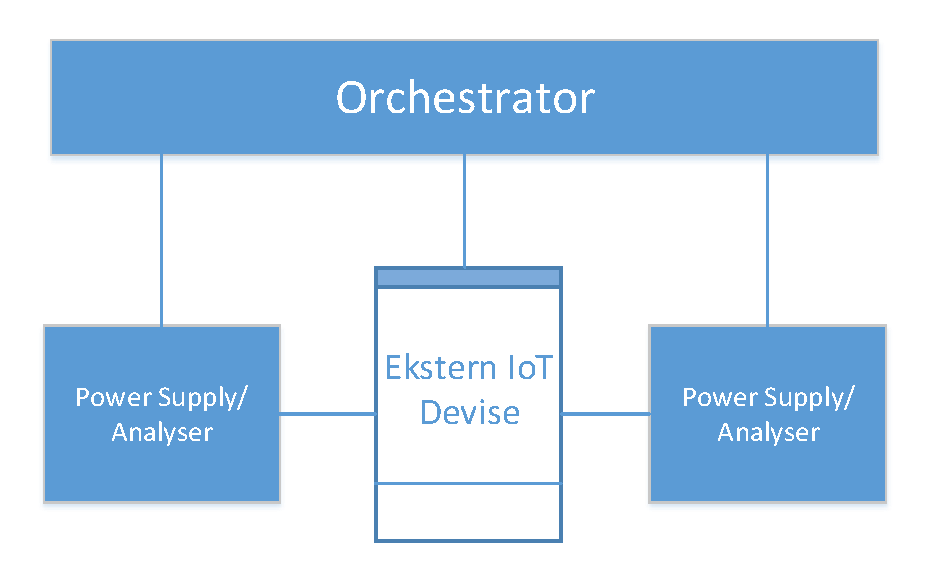
\includegraphics[width=0.5\textwidth]{figures/IPE_test_setup.pdf}
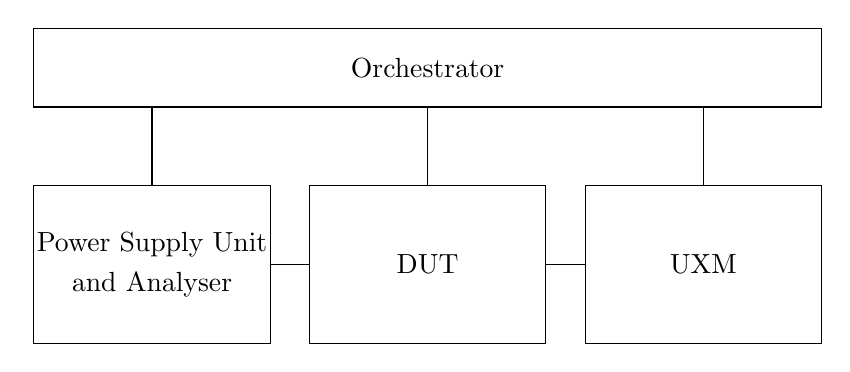
\begin{tikzpicture}
\draw  (-3.5,3) rectangle (6.5,2);
\draw  (-3.5,1) rectangle (-0.5,-1);
\draw  (0,1) rectangle (3,-1);
\draw  (3.5,1) rectangle (6.5,-1);
\node at (-2,0.25) {Power Supply Unit };
\node at (-2,-0.25) {and Analyser};
\node at (1.5,0) {DUT};
\node at (5,0) {UXM};
\node at (1.5,2.5) {Orchestrator};
\draw (-2,2) -- (-2,1);
\draw (1.5,2) -- (1.5,1);
\draw (5,2) -- (5,1);
\draw (-0.5,0) -- (0,0);
\draw(3,0) -- (3.5,0);
\end{tikzpicture}
\caption{Setup used to test for the power efficiency of the \gls{DUT}'s}
\label{fig:IPE_test_setup}
\end{figure}


As seen in \autoref{fig:IPE_test_setup}, an orchestrator, in this case \gls{TAP}, maintains the system. The orchestrator has a \gls{LAN} connection with the \gls{PSU} and the UXM and in this case a serial connection with the DUT. The \gls{PSU}s connection with the DUT is wires used to power on and analyse the power consumption of the device. It should be noted that the \gls{DUT} in question have two power inputs, one for the device power and one for the RF modem power, here only the modem is connected to the power analyser. The DUT is connected to the UXM using RF SMA cables.

\gls{TAP} is a software developed by Keysight Technologies which enables quick and easy access to the computers external connection. It also allows for C\# features to be used in the test design, meaning test steps can and has been designed to enable functionalities of the instruments. This includes for instance cell activation of the UXM and data collection from the PSU among other key functionalities, this couple with the ability to use loops, parallel test steps, serial com ports and batch scripts make this a very strong tool in designing, controlling and performing measurements. \citep{TAP} 

The \gls{PSU} is a N6705C DC Power Analyzer with the internal module 2Q SMU-BDA it has a range of 20 V and 3 A with a max output of 20 W. When getting data from the PSU it can be done in a couple different ways, but here it is stored in the internal RAM of the PSU before download. This though has a limitation of 512.000 data points per capture. \citep{PSU}

The base station is a E7515A UXM Wireless Test Set from Keysight Technologies which is able to emulate, both LTE and NB-IoT conditions. It features most of the functionalities in the NB-IoT protocol until release 13. It has a multitude of changeable parameters with easy access through a SCPI interface. \citep{UXM}

The initial settings of each component in the system can be seen in \autoref{tab:setup_parameters}.

\begin{table}[H]
\captionsetup{belowskip=0em}
\noindent
\centering
%\resizebox{!}{0.5\textheight}{
\begin{minipage}[t]{0.48\textwidth}
\begin{tabular}{|p{4cm}|p{2cm}|} \hline
\multicolumn{2}{|c|}{\textbf{Ekstern IoT device}}   \\ \hline
DL\_EARFCN         & 6240           \\ \hline
Enable             & Off            \\ \hline
\multicolumn{2}{c}{}  \\ 
\multicolumn{2}{c}{}  \\ 
\end{tabular}
%\caption{Initial values of the parameters in the emulator.}
\end{minipage}% 
\hfill
\begin{minipage}[t]{0.48\textwidth}
\raggedleft
\begin{tabular}{|p{4cm}|p{2cm}|} \hline
\multicolumn{2}{|c|}{\textbf{Power Supply/Analyser}} \\ \hline
Ampere             & 2.5 A          \\ \hline
Enable             & Off            \\ \hline
Sample interval	   & 100 $\mu$s		\\ \hline
Volt               & 3.6 V          \\ \hline
\end{tabular}
%\caption{Initial values of the parameters in the emulator.}
%\label{tab:setup_parameters}
\vspace{1em}
\end{minipage}
\resizebox{\textwidth}{!}{
\begin{tabular}{|p{5cm}|p{3cm}|p{4cm}|p{3cm}|} \hline
\multicolumn{4}{|c|}{\textbf{UXM \gls{BSE}}} \\ \hline
Cell ID                   & 0        & Cell type              	& NB-IoT         \\ \hline
CP format                 & Normal   & DRX Start Offset       	& 0              \\ \hline
drx-ULRetransmissionTimer & 0        & Host cell DL\_EARFCN 	& 6240           \\ \hline
Idle eDRX Cycle     & 20480 subframes& Idle eDRX State        	& Off            \\ \hline
Inactivity Timer        & 8 NPDCCH subframes & Long DRX cycle   & 1024 subframes \\ \hline
MAC padding DL           & off       & Max Repetition NPDCCH 	& 4              \\ \hline
Number of cells          & 1         & onDuration Timer         & 4 NPDCCH subframes \\ \hline
Operation mode           & Standalone& Power Saving Mode		& Off            \\ \hline
PRB offset               & 0         &$P_{TX}$                  & 23 dBm         \\ \hline
\gls{PTW}                & 5120 subframes & Repetition NPDSCH   & 1              \\ \hline
Repetition NPRACH        & 1         & Repetition NPUSCH        & 1              \\ \hline
Retransmission Timer & 2 NPDCCH subframes & T3324 (DRX period)  & 10 s           \\ \hline
T3412 (PSM period)      & 10 s       & Tx power                 & -80 dB/per 15 kHz \\ \hline
\end{tabular}}
\caption{Initial values of the parameters in the emulator.}
\label{tab:setup_parameters}
\end{table}

The procedures to measure the different elements can be in \appref{app:test_procedures}. When the data is procured the energy, power and time is needed for different parts of the measurement and is calculated respectively as:

\begin{align}
E &= \int_{A_{start}}^{A_{end}} f(x) dx \label{eq:energy}\\
P &= \mathbf{E}(f(x)) \quad for \, A_{start} \leq x \leq A_{end} \label{eq:power} \\
T &=  A_{end} - A_{start} \label{eq:time}\\
\end{align}
\begin{where}
\va{$E$}{is the energy of area A}{J}
\va{$P$}{is the average power consumption of area A}{W} 
\va{$T$}{is the duration of area A}{s}
\va{$\mathbf{E}$(•)}{is the mean function}{1}
\va{f(x)}{is the data point at time x}{W}
\va{$A_{start}$}{is the start time of area A}{s}
\va{$A_{end}$}{is the end time of area A}{s}
\end{where}

%Four different kinds of idle mode exist for a NB-IoT device: \gls{cDRX}, \gls{DRX}, \gls{eDRX} and \gls{PSM}. It is chosen not to look into \gls{cDRX} due to an assumption of the device transmitting its data quickly and then going into deep sleep. 

%When the device is in idle mode most parameters lose their influence entirely. Because of this a whole new set of parameters should be considered. For the \gls{DRX} case the cycle period is important, while for \gls{eDRX} however a few parameter more should be considered such as the repetition of the DRX cycle and the eDRX cycle period. For \gls{PSM} its is also the DRX cycle period as well as the repetition of the DRX cycle as well as the PSM cycle time. This can be summed up to two different types of parameters: period lengths and repetition numbers. It is assumed that both of these parameters have a proportional relation to the energy consumption of the idle modes, this means that only a single instance of the power consumption is needed for these different idle modes to extrapolate from.






%\subsubsection{Device Power Consumption}
%
%To measure the device power, the power input to the device is used in the setup. The test is performed using the following procedure:
%
%\textbf{Test Procedure}
%\vspace{-1.5em}
%\begin{enumerate}
%\item Setup the \gls{DUT} as shown on \autoref{fig:IPE_test_setup}
%\item Put in settings as described in \autoref{tab:setup_parameters} and \autoref{tab:UXM_initial_values} 
%\item Turn on power supply 
%\item Measure power output over 2 min
%\item Save measurements as "<device>\_Power\_consumption"
%\item Turn off power supply
%\item Change to next \gls{DUT}
%\item Repeat step 1-7 for all \gls{DUT}s.
%\end{enumerate}
%
%\textbf{Results}\\
%\begin{table}[H]
%\centering
%\begin{tabular}{|c|c|c|c|}\hline
%\textbf{Device}	& Quectel	& Telit & Ublox \\ \hline
%$\mathbf{P_{device}}$	& & & \\ \hline
%\end{tabular}
%\caption{Average power consumption of the \gls{DUT}s}
%\label{tab:device_power_results}
%\end{table}

\section{Energy to Connect and Disconnect the DUT to the Cell} \label{sec:performance_attach}

The energy to connect and disconnect the DUT to the cell involves the elements $E_{sync}$, $E_{attach}$ and $E_{release}$. The procedure to measure these can be found in \appref{app:test_procedures}. The first step is to get an overview of the measurements, to do this an example of the raw data from a measurement is presented in \autoref{fig:Attach_raw}. The areas are related to the elements in order, area D is when the device has been release and is therefore not used.

\tikzsetnextfilename{Attach_raw}
\begin{figure}[H]
\centering
\begin{minipage}[tbp]{0.58\textwidth}
\resizebox{\textwidth}{!}{
% This file was created by matlab2tikz.
%
%The latest updates can be retrieved from
%  http://www.mathworks.com/matlabcentral/fileexchange/22022-matlab2tikz-matlab2tikz
%where you can also make suggestions and rate matlab2tikz.
%
\definecolor{mycolor1}{rgb}{0.00000,0.44700,0.74100}%
%
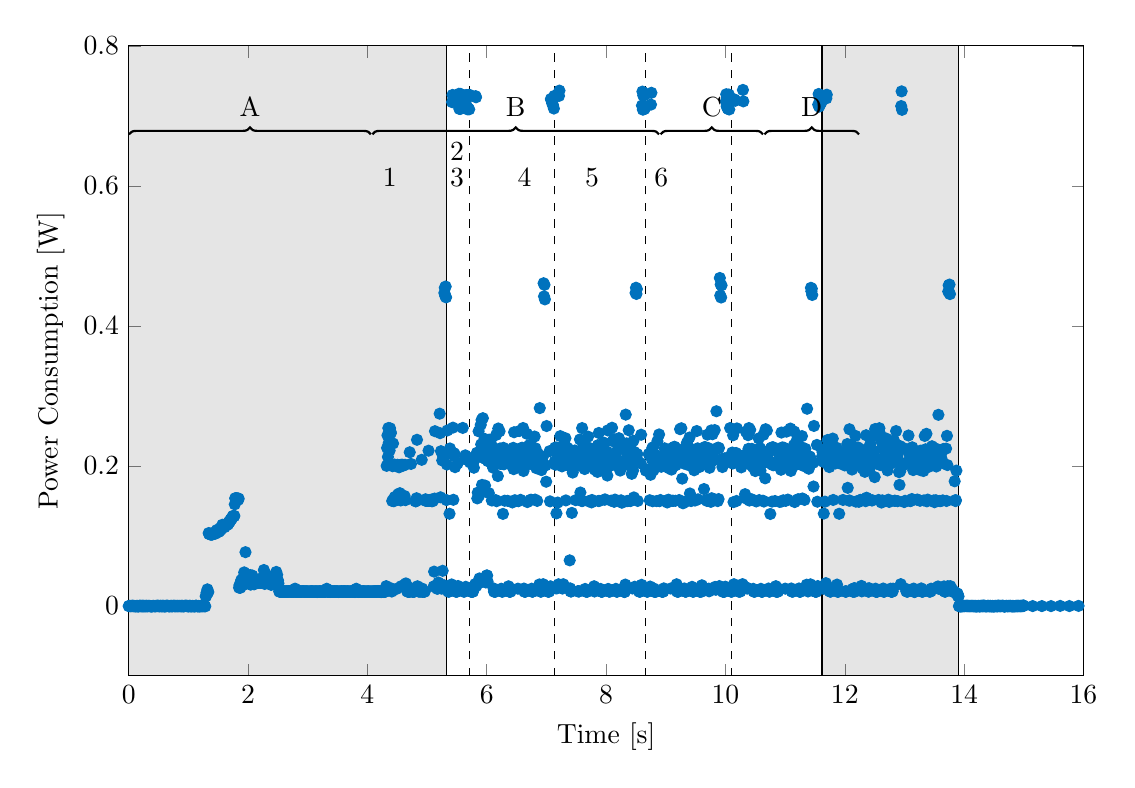
\begin{tikzpicture}
\begin{axis}[%
width=\textwidth,
height=0.66\textwidth,
at={(0.758in,0.481in)},
scale only axis,
xmin=0,
xmax=16,
xlabel={Time [s]},
ymin=-0.1,
ymax=0.8,
ylabel={Power Consumption [W]},
axis background/.style={fill=white}
]
\addplot [color=mycolor1,only marks,mark=*,mark options={solid},forget plot]
  table[row sep=crcr]{%
0	-0.00027465822\\
0.007168	-0.000137329092\\
0.014336	0\\
0.021504	-0.000137329092\\
0.028672	-0.000320435136\\
0.03584	-0.000160217568\\
0.043008	-0.000137329092\\
0.050176	-0.000137329092\\
0.057344	-4.5776088e-05\\
0.064512	-9.1553004e-05\\
0.07168	0.000205992828\\
0.078848	-0.00036621108\\
0.086016	-0.00027465822\\
0.093184	-0.000183106044\\
0.100352	-0.000251770572\\
0.10752	-0.00041198724\\
0.114688	-0.00057220488\\
0.121856	-0.000228882132\\
0.129024	-0.00041198724\\
0.136192	-4.5776088e-05\\
0.14336	4.5776088e-05\\
0.150528	-0.00059509332\\
0.157696	-0.00054931644\\
0.164864	-0.0006637572\\
0.172032	-0.000228882132\\
0.1792	-0.000114440652\\
0.186368	0.00034332192\\
0.193536	-0.000320435136\\
0.200704	-0.00018310518\\
0.207872	-4.5776916e-05\\
0.21504	-0.000183106044\\
0.222208	-0.00057220488\\
0.229376	0.000251769744\\
0.236544	-0.00048065184\\
0.243712	6.8664564e-05\\
0.25088	-0.00052642872\\
0.258048	-0.000228882132\\
0.265216	-2.28884616e-05\\
0.272384	-0.00043487568\\
0.279552	-0.000160217568\\
0.28672	-0.0004577634\\
0.293888	0.00018310518\\
0.301056	-0.000160217568\\
0.308224	-0.00054931644\\
0.315392	-0.000160217568\\
0.32256	-0.000205993656\\
0.329728	-4.5776088e-05\\
0.336896	-0.000228882132\\
0.344064	-0.000114440652\\
0.351232	-0.000160217568\\
0.3584	-0.000160217568\\
0.365568	-0.00045776412\\
0.372736	-0.00036621108\\
0.379904	-0.00061798104\\
0.387072	-0.00070953408\\
0.39424	-0.00043487568\\
0.401408	-9.1553004e-05\\
0.408576	-0.00027465822\\
0.415744	0\\
0.422912	-0.000160217568\\
0.43008	-0.000251769744\\
0.437248	-0.00057220488\\
0.444416	-0.00041198724\\
0.451584	-0.000160217568\\
0.458752	-0.000183106044\\
0.46592	-6.8664564e-05\\
0.473088	4.5776088e-05\\
0.480256	-0.000251769744\\
0.487424	0.0003890988\\
0.494592	-0.00018310518\\
0.50176	-0.000320434308\\
0.508928	2.28876264e-05\\
0.516096	-0.00043487568\\
0.523264	-0.00041198724\\
0.530432	-9.1553004e-05\\
0.5376	0.00016021674\\
0.544768	-0.00018310518\\
0.551936	-0.00029754666\\
0.559104	-0.0006637572\\
0.566272	0\\
0.57344	0.000114440652\\
0.580608	-0.000160217568\\
0.587776	-0.000160217568\\
0.594944	-0.0006637572\\
0.602112	-0.000183106044\\
0.60928	-0.00057220488\\
0.616448	-0.000137329092\\
0.623616	-0.000526428\\
0.630784	0.00018310518\\
0.637952	-6.8664564e-05\\
0.64512	9.1552176e-05\\
0.652288	0\\
0.659456	2.28876264e-05\\
0.666624	-0.000251770572\\
0.673792	-0.000343322748\\
0.68096	-0.0006637572\\
0.688128	-0.000160217568\\
0.695296	-0.000228882132\\
0.702464	0\\
0.709632	-0.0004577634\\
0.7168	-0.00029754666\\
0.723968	0.000114440652\\
0.731136	-0.0004577634\\
0.738304	-0.000343322748\\
0.745472	-0.000137329092\\
0.75264	4.5776088e-05\\
0.759808	0.000205993656\\
0.766976	-0.000343322748\\
0.774144	-0.000343322748\\
0.781312	4.5776088e-05\\
0.78848	-0.00029754666\\
0.795648	-0.00027465822\\
0.802816	4.5776088e-05\\
0.809984	-0.00041198724\\
0.817152	-9.1553004e-05\\
0.82432	2.28876264e-05\\
0.831488	-0.000228882132\\
0.838656	-0.0003890988\\
0.845824	-2.28884616e-05\\
0.852992	-0.000228882132\\
0.86016	-4.5776916e-05\\
0.867328	-0.000160217568\\
0.874496	-0.0004577634\\
0.881664	-0.000137329092\\
0.888832	-0.00029754666\\
0.896	0.00016021674\\
0.903168	-0.000343322748\\
0.910336	-0.0005950926\\
0.917504	-0.00027465822\\
0.924672	-0.00057220488\\
0.93184	-0.000114440652\\
0.939008	-4.5776916e-05\\
0.946176	9.1552176e-05\\
0.953344	0\\
0.960512	6.8664564e-05\\
0.96768	6.86637e-05\\
0.974848	-0.000160217568\\
0.982016	-4.5776088e-05\\
0.989184	-0.00054931644\\
0.996352	-0.00011444148\\
1.00352	-0.00050354028\\
1.010688	-0.000526428\\
1.017856	0.000137329092\\
1.025024	-0.000205993656\\
1.032192	0\\
1.03936	-0.00029754666\\
1.046528	-0.0005950926\\
1.053696	-0.00061798104\\
1.060864	-0.000205993656\\
1.068032	-0.000160217568\\
1.0752	-0.00011444148\\
1.082368	-0.000297545832\\
1.089536	-0.000343322748\\
1.096704	-0.0003890988\\
1.103872	-0.0003890988\\
1.11104	-0.00068664564\\
1.118208	0.00018310518\\
1.125376	0\\
1.132544	6.8664564e-05\\
1.139712	6.86637e-05\\
1.14688	-0.00036621108\\
1.154048	-0.00054931644\\
1.161216	-0.000343322748\\
1.168384	-0.000137329092\\
1.175552	-0.000228882132\\
1.18272	-0.00054931644\\
1.189888	-0.00068664564\\
1.197056	-0.00011444148\\
1.204224	-6.8664564e-05\\
1.211392	-0.00036621108\\
1.21856	-0.000343322748\\
1.225728	-0.00011444148\\
1.232896	-0.00018310518\\
1.240064	-0.000320435136\\
1.247232	-0.00027465822\\
1.2544	-0.000320434308\\
1.261568	0\\
1.268736	-0.000251770572\\
1.275904	-0.00027465822\\
1.283072	-0.00061798104\\
1.29024	0.0138244608\\
1.297408	0.0141448968\\
1.304576	0.0188598636\\
1.311744	0.0189056376\\
1.318912	0.023666382\\
1.32608	0.01966095\\
1.333248	0.0197753904\\
1.340416	0.104026788\\
1.347584	0.102653496\\
1.354752	0.102745044\\
1.36192	0.103019724\\
1.369088	0.102127068\\
1.376256	0.101989728\\
1.383424	0.103042584\\
1.390592	0.101966868\\
1.39776	0.101989728\\
1.404928	0.102287304\\
1.412096	0.104209884\\
1.419264	0.103248576\\
1.426432	0.103820796\\
1.4336	0.103729248\\
1.440768	0.104026788\\
1.447936	0.1036377\\
1.455104	0.103294368\\
1.462272	0.104301468\\
1.46944	0.105857856\\
1.476608	0.108352656\\
1.483776	0.105789168\\
1.490944	0.106361388\\
1.498112	0.105880752\\
1.50528	0.10583496\\
1.512448	0.106155396\\
1.519616	0.106979364\\
1.526784	0.10949706\\
1.533952	0.111213684\\
1.54112	0.108489996\\
1.548288	0.109909044\\
1.555456	0.110389716\\
1.562624	0.112197888\\
1.569792	0.11592864\\
1.57696	0.112907412\\
1.584128	0.11357118\\
1.591296	0.1131363\\
1.598464	0.11286162\\
1.605632	0.112472532\\
1.6128	0.115219116\\
1.619968	0.115173324\\
1.627136	0.114784236\\
1.634304	0.116249076\\
1.641472	0.116134632\\
1.64864	0.116455068\\
1.655808	0.11606598\\
1.662976	0.116546616\\
1.670144	0.118583676\\
1.677312	0.119773872\\
1.68448	0.119178756\\
1.691648	0.120826728\\
1.698816	0.12119292\\
1.705984	0.123046884\\
1.713152	0.123847956\\
1.72032	0.123870852\\
1.727488	0.124900812\\
1.734656	0.126319896\\
1.741824	0.12718962\\
1.748992	0.128585808\\
1.75616	0.128036484\\
1.763328	0.127967832\\
1.770496	0.128585808\\
1.777664	0.145133964\\
1.784832	0.1537857\\
1.792	0.153579708\\
1.799168	0.153396612\\
1.806336	0.1537857\\
1.813504	0.153099072\\
1.820672	0.15319062\\
1.82784	0.153396612\\
1.835008	0.151496892\\
1.842176	0.153327924\\
1.849344	0.0260238636\\
1.856512	0.0298919664\\
1.86368	0.0287704476\\
1.870848	0.0258865344\\
1.878016	0.028930662\\
1.885184	0.036781308\\
1.892352	0.0302352876\\
1.89952	0.037033092\\
1.906688	0.036186228\\
1.913856	0.0296630856\\
1.921024	0.0331649784\\
1.928192	0.042068484\\
1.93536	0.047904984\\
1.942528	0.0323638884\\
1.949696	0.037078848\\
1.956864	0.076766976\\
1.964032	0.0332336412\\
1.9712	0.039550788\\
1.978368	0.043601976\\
1.985536	0.03609468\\
1.992704	0.03588867\\
1.999872	0.0334854108\\
2.00704	0.0326614356\\
2.014208	0.03872682\\
2.021376	0.0359573364\\
2.028544	0.03362274\\
2.035712	0.044036856\\
2.04288	0.0303955056\\
2.050048	0.0336456288\\
2.057216	0.0338745096\\
2.064384	0.0335540772\\
2.071552	0.043395984\\
2.07872	0.038795472\\
2.085888	0.03362274\\
2.093056	0.036483768\\
2.100224	0.030830382\\
2.107392	0.0330047604\\
2.11456	0.0351333612\\
2.121728	0.0334396368\\
2.128896	0.0325927728\\
2.136064	0.034103394\\
2.143232	0.0331420896\\
2.1504	0.03552246\\
2.157568	0.0335998512\\
2.164736	0.0337371804\\
2.171904	0.0333938592\\
2.179072	0.03325653\\
2.18624	0.0359802252\\
2.193408	0.033782958\\
2.200576	0.0332336412\\
2.207744	0.0330505344\\
2.214912	0.033576966\\
2.22208	0.03588867\\
2.229248	0.0330505344\\
2.236416	0.033576966\\
2.243584	0.0338745096\\
2.250752	0.041152968\\
2.25792	0.0339660648\\
2.265088	0.051269544\\
2.272256	0.044403084\\
2.279424	0.031402584\\
2.286592	0.038314836\\
2.29376	0.0336456288\\
2.300928	0.038658132\\
2.308096	0.03918456\\
2.315264	0.0352706904\\
2.322432	0.0335082996\\
2.3296	0.0336685176\\
2.336768	0.042137136\\
2.343936	0.0346755996\\
2.351104	0.042503364\\
2.358272	0.038818368\\
2.36544	0.0344238264\\
2.372608	0.0319290156\\
2.379776	0.037147536\\
2.386944	0.0300292956\\
2.394112	0.0344924892\\
2.40128	0.0334396368\\
2.408448	0.0336456288\\
2.415616	0.0326614356\\
2.422784	0.0337142952\\
2.429952	0.0308761596\\
2.43712	0.03289032\\
2.444288	0.039367656\\
2.451456	0.03325653\\
2.458624	0.0337142952\\
2.465792	0.03362274\\
2.47296	0.048568716\\
2.480128	0.0314712504\\
2.487296	0.044471736\\
2.494464	0.0350189208\\
2.501632	0.036506664\\
2.5088	0.0321578964\\
2.515968	0.0257949828\\
2.523136	0.0204162588\\
2.530304	0.0205306992\\
2.537472	0.020553588\\
2.54464	0.0205078104\\
2.551808	0.0208053576\\
2.558976	0.0205306992\\
2.566144	0.0203704812\\
2.573312	0.0203247072\\
2.58048	0.02039337\\
2.587648	0.0206222508\\
2.594816	0.020553588\\
2.601984	0.020874024\\
2.609152	0.0201187116\\
2.61632	0.020553588\\
2.623488	0.0205078104\\
2.630656	0.0204162588\\
2.637824	0.0205306992\\
2.644992	0.0205764768\\
2.65216	0.0207366948\\
2.659328	0.0204162588\\
2.666496	0.0201644892\\
2.673664	0.0207366948\\
2.680832	0.0208511352\\
2.688	0.0205764768\\
2.695168	0.0206909172\\
2.702336	0.02039337\\
2.709504	0.020874024\\
2.716672	0.0205306992\\
2.72384	0.0202789296\\
2.731008	0.0207824688\\
2.738176	0.0205306992\\
2.745344	0.0209426868\\
2.752512	0.0203704812\\
2.75968	0.0204620364\\
2.766848	0.020347596\\
2.774016	0.020874024\\
2.781184	0.0204620364\\
2.788352	0.0246505752\\
2.79552	0.02039337\\
2.802688	0.0204620364\\
2.809856	0.0210113532\\
2.817024	0.020187378\\
2.824192	0.0206680284\\
2.83136	0.0205993656\\
2.838528	0.020553588\\
2.845696	0.0203018184\\
2.852864	0.0205993656\\
2.860032	0.0206222544\\
2.8672	0.020713806\\
2.874368	0.0203475924\\
2.881536	0.0208053576\\
2.888704	0.0203247072\\
2.895872	0.0201644892\\
2.90304	0.0205764768\\
2.910208	0.0208282464\\
2.917376	0.0208053576\\
2.924544	0.0207595836\\
2.931712	0.0205078104\\
2.93888	0.0204162588\\
2.946048	0.020553588\\
2.953216	0.0204620364\\
2.960384	0.0206222508\\
2.967552	0.0205306992\\
2.97472	0.0205993656\\
2.981888	0.0204620364\\
2.989056	0.0207366948\\
2.996224	0.020347596\\
3.003392	0.0204849252\\
3.01056	0.0204162588\\
3.017728	0.0203475924\\
3.024896	0.0203018184\\
3.032064	0.0202560408\\
3.039232	0.0204620364\\
3.0464	0.020713806\\
3.053568	0.0204162588\\
3.060736	0.0203018184\\
3.067904	0.0208969128\\
3.075072	0.020553588\\
3.08224	0.0205306992\\
3.089408	0.0204849252\\
3.096576	0.02039337\\
3.103744	0.0204162588\\
3.110912	0.0201416004\\
3.11808	0.0206909172\\
3.125248	0.0205764768\\
3.132416	0.0203247072\\
3.139584	0.020347596\\
3.146752	0.0207595836\\
3.15392	0.0200500488\\
3.161088	0.020713806\\
3.168256	0.0200042712\\
3.175424	0.0203247072\\
3.182592	0.0205764768\\
3.18976	0.0202560408\\
3.196928	0.020713806\\
3.204096	0.0208053576\\
3.211264	0.020187378\\
3.218432	0.0204391476\\
3.2256	0.0205306992\\
3.232768	0.02039337\\
3.239936	0.0203247072\\
3.247104	0.0207366948\\
3.254272	0.020713806\\
3.26144	0.020553588\\
3.268608	0.0203475924\\
3.275776	0.0203247072\\
3.282944	0.020072934\\
3.290112	0.0204849216\\
3.29728	0.0205993656\\
3.304448	0.0206451396\\
3.311616	0.0208053576\\
3.318784	0.024513246\\
3.325952	0.0209655756\\
3.33312	0.0205764768\\
3.340288	0.0202102632\\
3.347456	0.0200729376\\
3.354624	0.0202102668\\
3.361792	0.0203247072\\
3.36896	0.0202102668\\
3.376128	0.0206451396\\
3.383296	0.02002716\\
3.390464	0.0204620364\\
3.397632	0.0208282464\\
3.4048	0.0204391476\\
3.411968	0.020713806\\
3.419136	0.020233152\\
3.426304	0.0207595836\\
3.433472	0.0203704812\\
3.44064	0.0203704812\\
3.447808	0.0206909172\\
3.454976	0.0207824688\\
3.462144	0.020347596\\
3.469312	0.0204849252\\
3.47648	0.0205993656\\
3.483648	0.020553588\\
3.490816	0.0208053576\\
3.497984	0.0204162588\\
3.505152	0.0206680284\\
3.51232	0.0204162588\\
3.519488	0.0199584936\\
3.526656	0.0200729376\\
3.533824	0.0206222544\\
3.540992	0.02039337\\
3.54816	0.0205078104\\
3.555328	0.0204391476\\
3.562496	0.0204849216\\
3.569664	0.0209655756\\
3.576832	0.0204391476\\
3.584	0.0202789296\\
3.591168	0.020233152\\
3.598336	0.0204620364\\
3.605504	0.020874024\\
3.612672	0.020713806\\
3.61984	0.020713806\\
3.627008	0.0206909172\\
3.634176	0.0202789296\\
3.641344	0.0205306992\\
3.648512	0.0203018184\\
3.65568	0.0205306992\\
3.662848	0.0204391476\\
3.670016	0.0208511352\\
3.677184	0.0204620364\\
3.684352	0.0202789296\\
3.69152	0.0205993656\\
3.698688	0.0203475924\\
3.705856	0.0201187116\\
3.713024	0.0200729376\\
3.720192	0.0206680284\\
3.72736	0.0205764768\\
3.734528	0.0207824688\\
3.741696	0.020874024\\
3.748864	0.0204849216\\
3.756032	0.0201644892\\
3.7632	0.0202102668\\
3.770368	0.0208969128\\
3.777536	0.0204391476\\
3.784704	0.0200958228\\
3.791872	0.0199356084\\
3.79904	0.0204849252\\
3.806208	0.0232086168\\
3.813376	0.024513246\\
3.820544	0.0223388676\\
3.827712	0.020233152\\
3.83488	0.020553588\\
3.842048	0.0206222544\\
3.849216	0.0205306992\\
3.856384	0.02002716\\
3.863552	0.0206222544\\
3.87072	0.0202560408\\
3.877888	0.0202789296\\
3.885056	0.0205078104\\
3.892224	0.020187378\\
3.899392	0.0203018184\\
3.90656	0.0206451396\\
3.913728	0.02039337\\
3.920896	0.0202560408\\
3.928064	0.020919798\\
3.935232	0.0206222544\\
3.9424	0.0206909172\\
3.949568	0.0204620364\\
3.956736	0.0204162588\\
3.963904	0.020233152\\
3.971072	0.020553588\\
3.97824	0.0202560408\\
3.985408	0.0204391476\\
3.992576	0.0203247072\\
3.999744	0.0204391476\\
4.006912	0.020553588\\
4.01408	0.0207366948\\
4.021248	0.0205306992\\
4.028416	0.0204391476\\
4.035584	0.0203704812\\
4.042752	0.0203018184\\
4.04992	0.0201416004\\
4.057088	0.020713806\\
4.064256	0.020187378\\
4.071424	0.0204849216\\
4.078592	0.020187378\\
4.08576	0.0202102668\\
4.092928	0.0205764768\\
4.100096	0.0205993656\\
4.107264	0.0205764768\\
4.114432	0.0208053576\\
4.1216	0.0201416004\\
4.128768	0.0203247072\\
4.135936	0.0208282464\\
4.143104	0.0205993656\\
4.150272	0.0210571272\\
4.15744	0.0202102668\\
4.164608	0.0205306992\\
4.171776	0.0206909172\\
4.178944	0.0211715676\\
4.186112	0.020553588\\
4.19328	0.0206680284\\
4.200448	0.020553588\\
4.207616	0.0206680284\\
4.214784	0.020187378\\
4.221952	0.0204620364\\
4.22912	0.0197753904\\
4.236288	0.0206222544\\
4.243456	0.0205993656\\
4.250624	0.02039337\\
4.257792	0.0205764768\\
4.26496	0.0208511352\\
4.272128	0.0206222544\\
4.279296	0.02002716\\
4.286464	0.0207595836\\
4.293632	0.0204162588\\
4.3008	0.0206451396\\
4.307968	0.0205993656\\
4.315136	0.028244016\\
4.322304	0.200042712\\
4.329472	0.22570038\\
4.33664	0.243667584\\
4.343808	0.21283722\\
4.350976	0.254035944\\
4.358144	0.233001684\\
4.365312	0.245521512\\
4.37248	0.22190094\\
4.379648	0.253761264\\
4.386816	0.24895476\\
4.393984	0.246894804\\
4.401152	0.0249481188\\
4.40832	0.020553588\\
4.415488	0.149894712\\
4.422656	0.19953918\\
4.429824	0.232017516\\
4.436992	0.152389512\\
4.44416	0.14955138\\
4.451328	0.201919536\\
4.458496	0.155158992\\
4.465664	0.155754072\\
4.472832	0.200958264\\
4.48	0.19983672\\
4.487168	0.0242843616\\
4.494336	0.153282168\\
4.501504	0.201553344\\
4.508672	0.152458164\\
4.51584	0.159553512\\
4.523008	0.201095568\\
4.530176	0.197937\\
4.537344	0.151908876\\
4.544512	0.160995492\\
4.55168	0.201416004\\
4.558848	0.150627132\\
4.566016	0.0281753532\\
4.573184	0.153671256\\
4.580352	0.201782232\\
4.58752	0.155342088\\
4.594688	0.15319062\\
4.601856	0.200386044\\
4.609024	0.201347352\\
4.616192	0.15541074\\
4.62336	0.156967164\\
4.630528	0.201507552\\
4.637696	0.151062012\\
4.644864	0.0321807852\\
4.652032	0.0286331184\\
4.6592	0.0251998884\\
4.666368	0.0207366948\\
4.673536	0.0247421268\\
4.680704	0.020233152\\
4.687872	0.02039337\\
4.69504	0.024513246\\
4.702208	0.0201416004\\
4.709376	0.219451896\\
4.716544	0.024765012\\
4.723712	0.0205764768\\
4.73088	0.202812192\\
4.738048	0.0247879044\\
4.745216	0.0208969128\\
4.752384	0.0208053576\\
4.759552	0.0202789296\\
4.76672	0.0206680284\\
4.773888	0.02039337\\
4.781056	0.0206222544\\
4.788224	0.0207366948\\
4.795392	0.0206222508\\
4.80256	0.149734476\\
4.809728	0.149322492\\
4.816896	0.14984892\\
4.824064	0.153831456\\
4.831232	0.2372589\\
4.8384	0.028083798\\
4.845568	0.0246963492\\
4.852736	0.02419281\\
4.859904	0.0205306992\\
4.867072	0.0204849252\\
4.87424	0.0248336784\\
4.881408	0.0208511352\\
4.888576	0.020713806\\
4.895744	0.0246963492\\
4.902912	0.0204620364\\
4.91008	0.208671552\\
4.917248	0.0247421268\\
4.924416	0.020233152\\
4.931584	0.0205993656\\
4.938752	0.0211715676\\
4.94592	0.0205764768\\
4.953088	0.0205306992\\
4.960256	0.0203018184\\
4.967424	0.150489792\\
4.974592	0.15232086\\
4.98176	0.150260904\\
4.988928	0.150398244\\
4.996096	0.150306696\\
5.003264	0.150100704\\
5.010432	0.1502838\\
5.0176	0.150329592\\
5.024768	0.221717844\\
5.031936	0.150970464\\
5.039104	0.150489792\\
5.046272	0.151268004\\
5.05344	0.150352488\\
5.060608	0.151359552\\
5.067776	0.14998626\\
5.074944	0.151657092\\
5.082112	0.149528484\\
5.08928	0.151794432\\
5.096448	0.149734476\\
5.103616	0.15188598\\
5.110784	0.0278091432\\
5.117952	0.0489807\\
5.12512	0.153259272\\
5.132288	0.249572736\\
5.139456	0.0277862544\\
5.146624	0.0290222172\\
5.153792	0.0274429296\\
5.16096	0.0280609128\\
5.168128	0.024513246\\
5.175296	0.0252914436\\
5.182464	0.0249481188\\
5.189632	0.0333709704\\
5.1968	0.0303268428\\
5.203968	0.0296630856\\
5.211136	0.274566636\\
5.218304	0.246734604\\
5.225472	0.155136096\\
5.23264	0.221008284\\
5.239808	0.024879456\\
5.246976	0.0249023412\\
5.254144	0.207778932\\
5.261312	0.050148\\
5.26848	0.214508052\\
5.275648	0.213203448\\
5.282816	0.0295257564\\
5.289984	0.44702892\\
5.297152	0.4543992\\
5.30432	0.44274888\\
5.311488	0.4561614\\
5.318656	0.44068896\\
5.325824	0.151176456\\
5.332992	0.201942432\\
5.34016	0.250602696\\
5.347328	0.0230255136\\
5.354496	0.0205306992\\
5.361664	0.0205764768\\
5.368832	0.0204391476\\
5.376	0.131629932\\
5.383168	0.224876376\\
5.390336	0.0251312256\\
5.397504	0.219383244\\
5.404672	0.0239181516\\
5.41184	0.030670164\\
5.419008	0.71953596\\
5.426176	0.72981252\\
5.433344	0.254631024\\
5.440512	0.15158844\\
5.44768	0.218284596\\
5.454848	0.21416472\\
5.462016	0.216911304\\
5.469184	0.198188784\\
5.476352	0.0205078104\\
5.48352	0.0205306992\\
5.490688	0.0206222508\\
5.497856	0.020553588\\
5.505024	0.020553588\\
5.512192	0.203590404\\
5.51936	0.0284271228\\
5.526528	0.71548452\\
5.533696	0.73143756\\
5.540864	0.7099686\\
5.548032	0.72892008\\
5.5552	0.70976268\\
5.562368	0.73123164\\
5.569536	0.71083836\\
5.576704	0.72988128\\
5.583872	0.71276076\\
5.59104	0.0250167816\\
5.598208	0.254241936\\
5.605376	0.0242843616\\
5.612544	0.0203704812\\
5.619712	0.0208969128\\
5.62688	0.0204391476\\
5.634048	0.209701548\\
5.641216	0.215057376\\
5.648384	0.0272827152\\
5.655552	0.72972108\\
5.66272	0.7143174\\
5.669888	0.72569268\\
5.677056	0.709236\\
5.684224	0.72921744\\
5.691392	0.71058636\\
5.69856	0.72985824\\
5.705728	0.70925904\\
5.712896	0.72990432\\
5.720064	0.204917904\\
5.727232	0.0245819088\\
5.7344	0.0204391476\\
5.741568	0.0202789296\\
5.748736	0.020553588\\
5.755904	0.0202789296\\
5.763072	0.020347596\\
5.77024	0.0204849252\\
5.777408	0.205810524\\
5.784576	0.197364816\\
5.791744	0.208534248\\
5.798912	0.213386544\\
5.80608	0.0312652548\\
5.813248	0.72809604\\
5.820416	0.72649368\\
5.827584	0.0285873408\\
5.834752	0.218719476\\
5.84192	0.153579708\\
5.849088	0.16181946\\
5.856256	0.213203448\\
5.863424	0.249435396\\
5.870592	0.157241808\\
5.87776	0.039253248\\
5.884928	0.0331192008\\
5.892096	0.216224676\\
5.899264	0.258567804\\
5.906432	0.230712876\\
5.9136	0.265663152\\
5.920768	0.172828692\\
5.927936	0.21196746\\
5.935104	0.268157952\\
5.942272	0.224601732\\
5.94944	0.168914808\\
5.956608	0.21986388\\
5.963776	0.238609296\\
5.970944	0.17191314\\
5.978112	0.209976192\\
5.98528	0.0334854108\\
5.992448	0.041770944\\
5.999616	0.043533324\\
6.006784	0.043373124\\
6.013952	0.0349731432\\
6.02112	0.20670318\\
6.028288	0.235450728\\
6.035456	0.161132796\\
6.042624	0.237464892\\
6.049792	0.223205544\\
6.05696	0.235656756\\
6.064128	0.208557108\\
6.071296	0.231445296\\
6.078464	0.227508552\\
6.085632	0.150581376\\
6.0928	0.20100402\\
6.099968	0.225082404\\
6.107136	0.197410572\\
6.114304	0.0249481188\\
6.121472	0.02039337\\
6.12864	0.0207595836\\
6.135808	0.0204391476\\
6.142976	0.0201644892\\
6.150144	0.151130664\\
6.157312	0.244239804\\
6.16448	0.149574276\\
6.171648	0.210227976\\
6.178816	0.215835552\\
6.185984	0.185485824\\
6.193152	0.253417968\\
6.20032	0.207206712\\
6.207488	0.22279356\\
6.214656	0.249435396\\
6.221824	0.224853516\\
6.228992	0.202995288\\
6.23616	0.202926636\\
6.243328	0.024513246\\
6.250496	0.0206222544\\
6.257664	0.0208511352\\
6.264832	0.0202560408\\
6.272	0.131446836\\
6.279168	0.22583772\\
6.286336	0.202239972\\
6.293504	0.221946696\\
6.300672	0.150260904\\
6.30784	0.21956634\\
6.315008	0.204849252\\
6.322176	0.22000122\\
6.329344	0.20803068\\
6.336512	0.214210512\\
6.34368	0.211257936\\
6.350848	0.1501236\\
6.358016	0.213912972\\
6.365184	0.0280151352\\
6.372352	0.0207366948\\
6.37952	0.0204162588\\
6.386688	0.0204162588\\
6.393856	0.0203018184\\
6.401024	0.0207366948\\
6.408192	0.0245361312\\
6.41536	0.223457328\\
6.422528	0.200798028\\
6.429696	0.147811896\\
6.436864	0.20070648\\
6.444032	0.225791928\\
6.4512	0.195350652\\
6.458368	0.248085036\\
6.465536	0.150833124\\
6.472704	0.223022448\\
6.479872	0.202857948\\
6.48704	0.15042114\\
6.494208	0.206085204\\
6.501376	0.217620828\\
6.508544	0.207344052\\
6.515712	0.21372984\\
6.52288	0.0246505752\\
6.530048	0.149574276\\
6.537216	0.216247536\\
6.544384	0.249755868\\
6.551552	0.217918404\\
6.55872	0.206886276\\
6.565888	0.151542648\\
6.573056	0.205169688\\
6.580224	0.225494388\\
6.587392	0.2039337\\
6.59456	0.22586058\\
6.601728	0.201782232\\
6.608896	0.254104596\\
6.616064	0.192695616\\
6.623232	0.0247879044\\
6.6304	0.0204162588\\
6.637568	0.0204391476\\
6.644736	0.0203247072\\
6.651904	0.0206222544\\
6.659072	0.201187116\\
6.66624	0.219406104\\
6.673408	0.245841984\\
6.680576	0.148338324\\
6.687744	0.207115164\\
6.694912	0.215515116\\
6.70208	0.205078104\\
6.709248	0.229248036\\
6.716416	0.21503448\\
6.723584	0.229980456\\
6.730752	0.151496892\\
6.73792	0.207778932\\
6.745088	0.151542648\\
6.752256	0.02455902\\
6.759424	0.0204162588\\
6.766592	0.02039337\\
6.77376	0.0207366948\\
6.780928	0.0209884644\\
6.788096	0.201210012\\
6.795264	0.215309124\\
6.802432	0.2419281\\
6.8096	0.151863084\\
6.816768	0.225173952\\
6.823936	0.201667788\\
6.831104	0.196723944\\
6.838272	0.207412704\\
6.84544	0.149963364\\
6.852608	0.204574572\\
6.859776	0.217323288\\
6.866944	0.206932068\\
6.874112	0.195991524\\
6.88128	0.0306472752\\
6.888448	0.282531708\\
6.895616	0.0248107896\\
6.902784	0.0204162588\\
6.909952	0.02039337\\
6.91712	0.19397736\\
6.924288	0.0274200444\\
6.931456	0.20553588\\
6.938624	0.212745672\\
6.945792	0.0310134888\\
6.95296	0.46089936\\
6.960128	0.4420854\\
6.967296	0.4585878\\
6.974464	0.43782804\\
6.981632	0.027717588\\
6.9888	0.200775132\\
6.995968	0.177406308\\
7.003136	0.256919832\\
7.010304	0.0212860116\\
7.017472	0.0211486824\\
7.02464	0.0204849252\\
7.031808	0.0206451396\\
7.038976	0.0203704812\\
7.046144	0.0206451396\\
7.053312	0.221054076\\
7.06048	0.149322492\\
7.067648	0.0280151352\\
7.074816	0.72404496\\
7.081984	0.72248832\\
7.089152	0.72246564\\
7.09632	0.71784216\\
7.103488	0.72447984\\
7.110656	0.71514144\\
7.117824	0.72576144\\
7.124992	0.71040348\\
7.13216	0.72846216\\
7.139328	0.206382744\\
7.146496	0.226203912\\
7.153664	0.201644892\\
7.160832	0.0249710076\\
7.168	0.132179256\\
7.175168	0.226203912\\
7.182336	0.0253601064\\
7.189504	0.1476288\\
7.196672	0.212470992\\
7.20384	0.0308990484\\
7.211008	0.72843948\\
7.218176	0.73599228\\
7.225344	0.0274429296\\
7.232512	0.242546076\\
7.23968	0.213455196\\
7.246848	0.218124396\\
7.254016	0.216407772\\
7.261184	0.199310292\\
7.268352	0.0247879044\\
7.27552	0.0277404768\\
7.282688	0.0309677112\\
7.289856	0.029617308\\
7.297024	0.230781564\\
7.304192	0.215538012\\
7.31136	0.22952268\\
7.318528	0.239524848\\
7.325696	0.150695784\\
7.332864	0.201782232\\
7.340032	0.226181016\\
7.3472	0.202766436\\
7.354368	0.225425736\\
7.361536	0.200958264\\
7.368704	0.223869312\\
7.375872	0.214416504\\
7.38304	0.22235868\\
7.390208	0.065071116\\
7.397376	0.0250625628\\
7.404544	0.0207824688\\
7.411712	0.0207824688\\
7.41888	0.0207595836\\
7.426048	0.13286592\\
7.433216	0.213340752\\
7.440384	0.190452564\\
7.447552	0.215423568\\
7.45472	0.208328256\\
7.461888	0.218559276\\
7.469056	0.2062683\\
7.476224	0.221992488\\
7.483392	0.20436858\\
7.49056	0.151039116\\
7.497728	0.202880844\\
7.504896	0.21503448\\
7.512064	0.201965328\\
7.519232	0.200180052\\
7.5264	0.0208053576\\
7.533568	0.0211029048\\
7.540736	0.0208053576\\
7.547904	0.0206909172\\
7.555072	0.200683584\\
7.56224	0.237762432\\
7.569408	0.16197966\\
7.576576	0.218719476\\
7.583744	0.205879212\\
7.590912	0.149803164\\
7.59808	0.254013048\\
7.605248	0.149894712\\
7.612416	0.212860116\\
7.619584	0.230575572\\
7.626752	0.215583804\\
7.63392	0.208785996\\
7.641088	0.195510852\\
7.648256	0.0242614728\\
7.655424	0.0206909172\\
7.662592	0.0206222544\\
7.66976	0.0206222544\\
7.676928	0.0208282464\\
7.684096	0.0203704812\\
7.691264	0.0206909172\\
7.698432	0.24179076\\
7.7056	0.149528484\\
7.712768	0.22586058\\
7.719936	0.200546244\\
7.727104	0.199928268\\
7.734272	0.206886276\\
7.74144	0.22263336\\
7.748608	0.203155524\\
7.755776	0.147880548\\
7.762944	0.151336656\\
7.770112	0.149917608\\
7.77728	0.2170944\\
7.784448	0.149528484\\
7.791616	0.211326588\\
7.798784	0.0280838016\\
7.805952	0.0205993656\\
7.81312	0.194457996\\
7.820288	0.219612096\\
7.827456	0.207344052\\
7.834624	0.221214276\\
7.841792	0.205284132\\
7.84896	0.223297128\\
7.856128	0.191390976\\
7.863296	0.229591368\\
7.870464	0.149871816\\
7.877632	0.247032144\\
7.8848	0.149894712\\
7.891968	0.226272564\\
7.899136	0.194503788\\
7.906304	0.0242843616\\
7.913472	0.0205078104\\
7.92064	0.0208282464\\
7.927808	0.0203018184\\
7.934976	0.0203018184\\
7.942144	0.20086668\\
7.949312	0.218353284\\
7.95648	0.207984924\\
7.963648	0.233184816\\
7.970816	0.15174864\\
7.977984	0.21256254\\
7.985152	0.15204618\\
7.99232	0.211280832\\
7.999488	0.21839904\\
8.006656	0.207458496\\
8.013824	0.220573404\\
8.020992	0.186195384\\
8.02816	0.25069428\\
8.035328	0.0242843616\\
8.042496	0.020874024\\
8.049664	0.0206451396\\
8.056832	0.0206451396\\
8.064	0.0204620364\\
8.071168	0.200546244\\
8.078336	0.200431836\\
8.085504	0.150306696\\
8.092672	0.205787664\\
8.09984	0.254470824\\
8.107008	0.202514652\\
8.114176	0.235267632\\
8.121344	0.206291196\\
8.128512	0.238151556\\
8.13568	0.148704516\\
8.142848	0.214988724\\
8.150016	0.151863084\\
8.157184	0.215263368\\
8.164352	0.0243759168\\
8.17152	0.0206222544\\
8.178688	0.0205764768\\
8.185856	0.0203018184\\
8.193024	0.22263336\\
8.200192	0.207481392\\
8.20736	0.224166852\\
8.214528	0.2395935\\
8.221696	0.224807724\\
8.228864	0.207092268\\
8.236032	0.193290696\\
8.2432	0.203018184\\
8.250368	0.150810228\\
8.257536	0.201095568\\
8.264704	0.147399912\\
8.271872	0.201164256\\
8.27904	0.224327088\\
8.286208	0.0246734604\\
8.293376	0.020553588\\
8.300544	0.0205078104\\
8.307712	0.0198898308\\
8.31488	0.0201416004\\
8.322048	0.030464172\\
8.329216	0.27321624\\
8.336384	0.0249710076\\
8.343552	0.232154856\\
8.35072	0.149711616\\
8.357888	0.216911304\\
8.365056	0.149894712\\
8.372224	0.22162626\\
8.379392	0.250900272\\
8.38656	0.223571772\\
8.393728	0.203521716\\
8.400896	0.214485156\\
8.408064	0.149734476\\
8.415232	0.230758632\\
8.4224	0.201805128\\
8.429568	0.188644392\\
8.436736	0.195259104\\
8.443904	0.0249252336\\
8.451072	0.1932678\\
8.45824	0.235908504\\
8.465408	0.154975896\\
8.472576	0.21986388\\
8.479744	0.0273742668\\
8.486912	0.205261236\\
8.49408	0.44709768\\
8.501248	0.45444492\\
8.508416	0.44561016\\
8.515584	0.45256788\\
8.522752	0.216842652\\
8.52992	0.149963364\\
8.537088	0.206062308\\
8.544256	0.0251083368\\
8.551424	0.0208511352\\
8.558592	0.0203247072\\
8.56576	0.0206909172\\
8.572928	0.0205306992\\
8.580096	0.203659056\\
8.587264	0.244514448\\
8.594432	0.0300979584\\
8.6016	0.7146378\\
8.608768	0.73457352\\
8.615936	0.70882416\\
8.623104	0.72889704\\
8.630272	0.70953372\\
8.63744	0.73075104\\
8.644608	0.70985412\\
8.651776	0.72990432\\
8.658944	0.7124634\\
8.666112	0.19324494\\
8.67328	0.024513246\\
8.680448	0.0209426868\\
8.687616	0.0202102668\\
8.694784	0.0207366948\\
8.701952	0.0208511352\\
8.70912	0.194915772\\
8.716288	0.2170944\\
8.723456	0.215698248\\
8.730624	0.150970464\\
8.737792	0.0276260364\\
8.74496	0.187293996\\
8.752128	0.7160112\\
8.759296	0.73287972\\
8.766464	0.209747304\\
8.773632	0.225379944\\
8.7808	0.149528484\\
8.787968	0.226615896\\
8.795136	0.193954464\\
8.802304	0.0248107896\\
8.809472	0.0201187116\\
8.81664	0.0205078104\\
8.823808	0.0202789296\\
8.830976	0.020187378\\
8.838144	0.198623664\\
8.845312	0.149757372\\
8.85248	0.205490124\\
8.859648	0.235427832\\
8.866816	0.20800782\\
8.873984	0.214096068\\
8.881152	0.203567508\\
8.88832	0.244926468\\
8.895488	0.149642928\\
8.902656	0.20919798\\
8.909824	0.151245108\\
8.916992	0.206909172\\
8.92416	0.198783864\\
8.931328	0.0209884644\\
8.938496	0.0201187116\\
8.945664	0.0206680284\\
8.952832	0.0202560408\\
8.96	0.0208053576\\
8.967168	0.0250625628\\
8.974336	0.204551712\\
8.981504	0.225105264\\
8.988672	0.200729376\\
8.99584	0.213935832\\
9.003008	0.201553344\\
9.010176	0.150398244\\
9.017344	0.203956596\\
9.024512	0.147743208\\
9.03168	0.205558776\\
9.038848	0.217712412\\
9.046016	0.151702884\\
9.053184	0.196632396\\
9.060352	0.212814324\\
9.06752	0.211578372\\
9.074688	0.214942932\\
9.081856	0.0248565672\\
9.089024	0.221397408\\
9.096192	0.194686884\\
9.10336	0.222175584\\
9.110528	0.150100704\\
9.117696	0.225952128\\
9.124864	0.150077808\\
9.132032	0.225631728\\
9.1392	0.20407104\\
9.146368	0.227371212\\
9.153536	0.20084382\\
9.160704	0.150146496\\
9.167872	0.200935368\\
9.17504	0.225196812\\
9.182208	0.0309448224\\
9.189376	0.0205078104\\
9.196544	0.0205078104\\
9.203712	0.0204849252\\
9.21088	0.02039337\\
9.218048	0.216522216\\
9.225216	0.151176456\\
9.232384	0.214714044\\
9.239552	0.252433764\\
9.24672	0.21166992\\
9.253888	0.214416504\\
9.261056	0.253761264\\
9.268224	0.219657888\\
9.275392	0.181800828\\
9.28256	0.221214276\\
9.289728	0.146575908\\
9.296896	0.22350312\\
9.304064	0.203384412\\
9.311232	0.0249023412\\
9.3184	0.020919798\\
9.325568	0.0205764768\\
9.332736	0.0205764768\\
9.339904	0.020347596\\
9.347072	0.204391476\\
9.35424	0.233001684\\
9.361408	0.20173644\\
9.368576	0.229270932\\
9.375744	0.150398244\\
9.382912	0.221534712\\
9.39008	0.150901776\\
9.397248	0.240509016\\
9.404416	0.160606368\\
9.411584	0.214828488\\
9.418752	0.210456864\\
9.42592	0.149780268\\
9.433088	0.206176752\\
9.440256	0.0272140488\\
9.447424	0.0205993656\\
9.454592	0.0206222544\\
9.46176	0.0204849252\\
9.468928	0.0205306992\\
9.476096	0.193748472\\
9.483264	0.209381112\\
9.490432	0.150535584\\
9.4976	0.20187378\\
9.504768	0.213890076\\
9.511936	0.20130156\\
9.519104	0.249778728\\
9.526272	0.2026062\\
9.53344	0.225036612\\
9.540608	0.152229312\\
9.547776	0.223411572\\
9.554944	0.202835088\\
9.562112	0.198326088\\
9.56928	0.020233152\\
9.576448	0.0208053576\\
9.583616	0.0206909172\\
9.590784	0.0205764768\\
9.597952	0.0208969128\\
9.60512	0.0294570936\\
9.612288	0.0208511352\\
9.619456	0.20874024\\
9.626624	0.21752928\\
9.633792	0.207344052\\
9.64096	0.16692354\\
9.648128	0.219245904\\
9.655296	0.227050776\\
9.662464	0.20363616\\
9.669632	0.206314092\\
9.6768	0.202331556\\
9.683968	0.151336656\\
9.691136	0.149963364\\
9.698304	0.244583136\\
9.705472	0.150444036\\
9.71264	0.225425736\\
9.719808	0.0246276828\\
9.726976	0.020874024\\
9.734144	0.197296128\\
9.741312	0.221855148\\
9.74848	0.204048144\\
9.755648	0.148635864\\
9.762816	0.250648488\\
9.769984	0.153831456\\
9.777152	0.207389808\\
9.78432	0.245269764\\
9.791488	0.214233408\\
9.798656	0.221122728\\
9.805824	0.152503956\\
9.812992	0.208419804\\
9.82016	0.251129124\\
9.827328	0.0271682712\\
9.834496	0.0233917236\\
9.841664	0.0232086168\\
9.848832	0.27804564\\
9.856	0.0251769996\\
9.863168	0.225173952\\
9.870336	0.149711616\\
9.877504	0.22613526\\
9.884672	0.152572644\\
9.89184	0.225425736\\
9.899008	0.0283126824\\
9.906176	0.4684068\\
9.913344	0.44332128\\
9.920512	0.45909108\\
9.92768	0.44048304\\
9.934848	0.45790092\\
9.942016	0.20990754\\
9.949184	0.198348984\\
9.956352	0.020233152\\
9.96352	0.0204849252\\
9.970688	0.0205078104\\
9.977856	0.0204162588\\
9.985024	0.0203247072\\
9.992192	0.2109375\\
9.99936	0.0274429296\\
10.006528	0.7204284\\
10.013696	0.7308198\\
10.020864	0.7136766\\
10.028032	0.72617328\\
10.0352	0.71067816\\
10.042368	0.72937764\\
10.049536	0.70960248\\
10.056704	0.73043064\\
10.063872	0.70912152\\
10.07104	0.025085448\\
10.078208	0.254035944\\
10.085376	0.0250396704\\
10.092544	0.0204620364\\
10.099712	0.0204162588\\
10.10688	0.0204391476\\
10.114048	0.219062808\\
10.121216	0.203361516\\
10.128384	0.243736236\\
10.135552	0.148269636\\
10.14272	0.0309677112\\
10.149888	0.72344988\\
10.157056	0.72251136\\
10.164224	0.72152712\\
10.171392	0.212882976\\
10.17856	0.218421936\\
10.185728	0.149871816\\
10.192896	0.253532412\\
10.200064	0.205009452\\
10.207232	0.0252227772\\
10.2144	0.020874024\\
10.221568	0.020874024\\
10.228736	0.0204849252\\
10.235904	0.0205078104\\
10.243072	0.0211029048\\
10.25024	0.0206222544\\
10.257408	0.200637828\\
10.264576	0.197868348\\
10.271744	0.205490124\\
10.278912	0.212516784\\
10.28608	0.0310821516\\
10.293248	0.73697652\\
10.300416	0.72063432\\
10.307584	0.0283126824\\
10.314752	0.211463928\\
10.32192	0.154289232\\
10.329088	0.1596222\\
10.336256	0.216155988\\
10.343424	0.248840316\\
10.350592	0.153877248\\
10.35776	0.0261154152\\
10.364928	0.0247421232\\
10.372096	0.209724408\\
10.379264	0.243873576\\
10.386432	0.22439574\\
10.3936	0.254013048\\
10.400768	0.150489792\\
10.407936	0.202102668\\
10.415104	0.251403804\\
10.422272	0.211143492\\
10.42944	0.152412408\\
10.436608	0.20173644\\
10.443776	0.224304192\\
10.450944	0.151817328\\
10.458112	0.19866942\\
10.46528	0.024398802\\
10.472448	0.0205993656\\
10.479616	0.0206680284\\
10.486784	0.02039337\\
10.493952	0.0204849252\\
10.50112	0.192581172\\
10.508288	0.212745672\\
10.515456	0.149230944\\
10.522624	0.214279164\\
10.529792	0.214508052\\
10.53696	0.21752928\\
10.544128	0.194778432\\
10.551296	0.22263336\\
10.558464	0.239227308\\
10.565632	0.151130664\\
10.5728	0.203727708\\
10.579968	0.225334152\\
10.587136	0.193153392\\
10.594304	0.024398802\\
10.601472	0.0205078104\\
10.60864	0.02039337\\
10.615808	0.020347596\\
10.622976	0.0205306992\\
10.630144	0.150215148\\
10.637312	0.244445796\\
10.64448	0.149093604\\
10.651648	0.220092768\\
10.658816	0.204917904\\
10.665984	0.182235708\\
10.673152	0.252410904\\
10.68032	0.216590868\\
10.687488	0.2110977\\
10.694656	0.250534044\\
10.701824	0.2144394\\
10.708992	0.21020508\\
10.71616	0.205101\\
10.723328	0.0248565672\\
10.730496	0.0206680284\\
10.737664	0.020553588\\
10.744832	0.0206222544\\
10.752	0.131332392\\
10.759168	0.224853516\\
10.766336	0.202926636\\
10.773504	0.226066572\\
10.780672	0.149002092\\
10.78784	0.226478556\\
10.795008	0.201095568\\
10.802176	0.226478556\\
10.809344	0.201072672\\
10.816512	0.2229309\\
10.82368	0.202812192\\
10.830848	0.149803164\\
10.838016	0.205032348\\
10.845184	0.028198242\\
10.852352	0.020233152\\
10.85952	0.0202789296\\
10.866688	0.0209884644\\
10.873856	0.020553588\\
10.881024	0.0205078104\\
10.888192	0.024719238\\
10.89536	0.21723174\\
10.902528	0.206520084\\
10.909696	0.148544316\\
10.916864	0.205444332\\
10.924032	0.222152688\\
10.9312	0.194457996\\
10.938368	0.247604364\\
10.945536	0.14925384\\
10.952704	0.226364112\\
10.959872	0.201599136\\
10.96704	0.150810228\\
10.974208	0.202629096\\
10.981376	0.225906372\\
10.988544	0.201370248\\
10.995712	0.213706944\\
11.00288	0.0246734604\\
11.010048	0.150077808\\
11.017216	0.205467228\\
11.024384	0.248931864\\
11.031552	0.20684052\\
11.03872	0.216430668\\
11.045888	0.151840188\\
11.053056	0.213615432\\
11.060224	0.214942932\\
11.067392	0.211830156\\
11.07456	0.216247536\\
11.081728	0.20800782\\
11.088896	0.253303524\\
11.096064	0.192787164\\
11.103232	0.024879456\\
11.1104	0.0207595836\\
11.117568	0.0205306992\\
11.124736	0.020713806\\
11.131904	0.0205306992\\
11.139072	0.200889576\\
11.14624	0.229476924\\
11.153408	0.249046308\\
11.160576	0.148338324\\
11.167744	0.201393144\\
11.174912	0.224075304\\
11.18208	0.20157624\\
11.189248	0.23519898\\
11.196416	0.205078104\\
11.203584	0.230163588\\
11.210752	0.152069076\\
11.21792	0.216384876\\
11.225088	0.152252172\\
11.232256	0.0249023412\\
11.239424	0.0206680284\\
11.246592	0.0201416004\\
11.25376	0.0207366948\\
11.260928	0.020553588\\
11.268096	0.205352784\\
11.275264	0.226547244\\
11.282432	0.242546076\\
11.2896	0.153442368\\
11.296768	0.224647524\\
11.303936	0.202651956\\
11.311104	0.199905372\\
11.318272	0.208053576\\
11.32544	0.151382448\\
11.332608	0.201347352\\
11.339776	0.22439574\\
11.346944	0.20130156\\
11.354112	0.199996956\\
11.36128	0.030303954\\
11.368448	0.281616192\\
11.375616	0.0249481188\\
11.382784	0.020713806\\
11.389952	0.0211944564\\
11.39712	0.195945732\\
11.404288	0.0276031512\\
11.411456	0.213546744\\
11.418624	0.212356548\\
11.425792	0.0308074932\\
11.43296	0.45433044\\
11.440128	0.44945532\\
11.447296	0.45309456\\
11.454464	0.44414532\\
11.461632	0.0273971556\\
11.4688	0.20434572\\
11.475968	0.170562744\\
11.483136	0.257057172\\
11.490304	0.0215835552\\
11.497472	0.0207595836\\
11.50464	0.0205306992\\
11.511808	0.0204391476\\
11.518976	0.020347596\\
11.526144	0.02039337\\
11.533312	0.229934664\\
11.54048	0.148841856\\
11.547648	0.0283355712\\
11.554816	0.71603388\\
11.561984	0.73118592\\
11.569152	0.71312724\\
11.57632	0.72665388\\
11.583488	0.7154388\\
11.590656	0.7244568\\
11.597824	0.71839152\\
11.604992	0.7189866\\
11.61216	0.72081756\\
11.619328	0.213317856\\
11.626496	0.219886776\\
11.633664	0.206085204\\
11.640832	0.02455902\\
11.648	0.131904612\\
11.655168	0.223113996\\
11.662336	0.0251083368\\
11.669504	0.148933404\\
11.676672	0.21283722\\
11.68384	0.0325241064\\
11.691008	0.72496044\\
11.698176	0.73020168\\
11.705344	0.024513246\\
11.712512	0.236984256\\
11.71968	0.201782232\\
11.726848	0.22263336\\
11.734016	0.202995288\\
11.741184	0.198280332\\
11.748352	0.0206451396\\
11.75552	0.0207366948\\
11.762688	0.020553588\\
11.769856	0.0208282464\\
11.777024	0.214393608\\
11.784192	0.21416472\\
11.79136	0.216476424\\
11.798528	0.239021316\\
11.805696	0.151359552\\
11.812864	0.20670318\\
11.820032	0.220573404\\
11.8272	0.20713806\\
11.834368	0.22396086\\
11.841536	0.203430168\\
11.848704	0.225288396\\
11.855872	0.214347852\\
11.86304	0.22586058\\
11.870208	0.030464172\\
11.877376	0.0202102668\\
11.884544	0.020874024\\
11.891712	0.0204620364\\
11.89888	0.0207595836\\
11.906048	0.131607036\\
11.913216	0.203659056\\
11.920384	0.210159288\\
11.927552	0.204528816\\
11.93472	0.218353284\\
11.941888	0.20700072\\
11.949056	0.21546936\\
11.956224	0.209060676\\
11.963392	0.212722776\\
11.97056	0.151359552\\
11.977728	0.209976192\\
11.984896	0.215057376\\
11.992064	0.207664488\\
11.999232	0.200683584\\
12.0064	0.0208282464\\
12.013568	0.0202102668\\
12.020736	0.0206680284\\
12.027904	0.0206680284\\
12.035072	0.201324456\\
12.04224	0.231216408\\
12.049408	0.168640128\\
12.056576	0.225883476\\
12.063744	0.200592036\\
12.070912	0.15042114\\
12.07808	0.252365112\\
12.085248	0.150398244\\
12.092416	0.203315724\\
12.099584	0.23023224\\
12.106752	0.204826356\\
12.11392	0.217918404\\
12.121088	0.194778432\\
12.128256	0.024032592\\
12.135424	0.0202789296\\
12.142592	0.0207366948\\
12.14976	0.0248336784\\
12.156928	0.02039337\\
12.164096	0.025405884\\
12.171264	0.0205078104\\
12.178432	0.242912268\\
12.1856	0.148933404\\
12.192768	0.222679152\\
12.199936	0.203956596\\
12.207104	0.204711912\\
12.214272	0.209266668\\
12.22144	0.226341252\\
12.228608	0.201484656\\
12.235776	0.14868162\\
12.242944	0.150192252\\
12.250112	0.150787368\\
12.25728	0.213340752\\
12.264448	0.1514511\\
12.271616	0.20274354\\
12.278784	0.028564452\\
12.285952	0.0207824688\\
12.29312	0.196632396\\
12.300288	0.209106432\\
12.307456	0.215423568\\
12.314624	0.209884644\\
12.321792	0.213111864\\
12.32896	0.212745672\\
12.336128	0.191528316\\
12.343296	0.223136892\\
12.350464	0.149620068\\
12.357632	0.243804924\\
12.3648	0.154541016\\
12.371968	0.222747804\\
12.379136	0.19367982\\
12.386304	0.024719238\\
12.393472	0.0204849252\\
12.40064	0.0204391476\\
12.407808	0.025245666\\
12.414976	0.0244674684\\
12.422144	0.197525016\\
12.429312	0.23155974\\
12.43648	0.209243772\\
12.443648	0.241882308\\
12.450816	0.15071868\\
12.457984	0.222610464\\
12.465152	0.150833124\\
12.47232	0.220916736\\
12.479488	0.206588736\\
12.486656	0.215812692\\
12.493824	0.209312424\\
12.500992	0.183952332\\
12.50816	0.252639756\\
12.515328	0.0246047976\\
12.522496	0.0202102668\\
12.529664	0.020187378\\
12.536832	0.0205306992\\
12.544	0.0203704812\\
12.551168	0.203361516\\
12.558336	0.202651956\\
12.565504	0.151336656\\
12.572672	0.208785996\\
12.57984	0.253807056\\
12.587008	0.201690648\\
12.594176	0.245338452\\
12.601344	0.201347352\\
12.608512	0.236297592\\
12.61568	0.14765166\\
12.622848	0.224990856\\
12.630016	0.150741576\\
12.637184	0.225036612\\
12.644352	0.0248336784\\
12.65152	0.020187378\\
12.658688	0.0205993656\\
12.665856	0.0206222544\\
12.673024	0.211944564\\
12.680192	0.216728208\\
12.68736	0.213363648\\
12.694528	0.239044176\\
12.701696	0.216155988\\
12.708864	0.208557108\\
12.716032	0.19354248\\
12.7232	0.208534248\\
12.730368	0.15172578\\
12.737536	0.204528816\\
12.744704	0.14852142\\
12.751872	0.20246886\\
12.75904	0.226272564\\
12.766208	0.02455902\\
12.773376	0.020713806\\
12.780544	0.0202102668\\
12.787712	0.0203704812\\
12.79488	0.0207595836\\
12.802048	0.0206222508\\
12.809216	0.0246505752\\
12.816384	0.22119138\\
12.823552	0.236412036\\
12.83072	0.150146496\\
12.837888	0.205719012\\
12.845056	0.150169356\\
12.852224	0.209976192\\
12.859392	0.249755868\\
12.86656	0.212928768\\
12.873728	0.211738572\\
12.880896	0.214485156\\
12.888064	0.149620068\\
12.895232	0.220756536\\
12.9024	0.207092268\\
12.909568	0.191047644\\
12.916736	0.172851552\\
12.923904	0.22835538\\
12.931072	0.192581172\\
12.93824	0.0310821516\\
12.945408	0.71392824\\
12.952576	0.73493964\\
12.959744	0.70852644\\
12.966912	0.225929268\\
12.97408	0.201232908\\
12.981248	0.22483062\\
12.988416	0.20203398\\
12.995584	0.148338324\\
13.002752	0.202583304\\
13.00992	0.150077808\\
13.017088	0.203704812\\
13.024256	0.0243759168\\
13.031424	0.0207366948\\
13.038592	0.0210571272\\
13.04576	0.02039337\\
13.052928	0.0204391476\\
13.060096	0.20553588\\
13.067264	0.24339294\\
13.074432	0.218421936\\
13.0816	0.206520084\\
13.088768	0.221397408\\
13.095936	0.149665824\\
13.103104	0.205306992\\
13.110272	0.150054912\\
13.11744	0.225769032\\
13.124608	0.152664192\\
13.131776	0.226478556\\
13.138944	0.201553344\\
13.146112	0.19400022\\
13.15328	0.0247421268\\
13.160448	0.02039337\\
13.167616	0.019866942\\
13.174784	0.0204849252\\
13.181952	0.0206680284\\
13.18912	0.196746804\\
13.196288	0.206291196\\
13.203456	0.216728208\\
13.210624	0.151817328\\
13.217792	0.214782732\\
13.22496	0.15158844\\
13.232128	0.195190416\\
13.239296	0.219932532\\
13.246464	0.209060676\\
13.253632	0.218765268\\
13.2608	0.150169356\\
13.267968	0.221717844\\
13.275136	0.193794228\\
13.282304	0.0250167852\\
13.289472	0.0204391476\\
13.29664	0.0205764768\\
13.303808	0.0205993656\\
13.310976	0.0205078104\\
13.318144	0.192718512\\
13.325312	0.15071868\\
13.33248	0.200935368\\
13.339648	0.24279786\\
13.346816	0.201370248\\
13.353984	0.223709112\\
13.361152	0.197662356\\
13.36832	0.245819088\\
13.375488	0.149368284\\
13.382656	0.217918404\\
13.389824	0.151817328\\
13.396992	0.215446464\\
13.40416	0.198577872\\
13.411328	0.0206451396\\
13.418496	0.0207824688\\
13.425664	0.020553588\\
13.432832	0.020874024\\
13.44	0.020713806\\
13.447168	0.0246276828\\
13.454336	0.208694448\\
13.461504	0.22805784\\
13.468672	0.203018184\\
13.47584	0.21533202\\
13.483008	0.202102668\\
13.490176	0.150650028\\
13.497344	0.201965328\\
13.504512	0.148132332\\
13.51168	0.201370248\\
13.518848	0.224922168\\
13.526016	0.150924672\\
13.533184	0.199150092\\
13.540352	0.203727708\\
13.54752	0.2204361\\
13.554688	0.204895008\\
13.561856	0.0278091432\\
13.569024	0.272941596\\
13.576192	0.0243759168\\
13.58336	0.211212144\\
13.590528	0.14982606\\
13.597696	0.216842652\\
13.604864	0.14968872\\
13.612032	0.216590868\\
13.6192	0.210708612\\
13.626368	0.22206114\\
13.633536	0.205101\\
13.640704	0.15071868\\
13.647872	0.20391084\\
13.65504	0.22423554\\
13.662208	0.027877806\\
13.669376	0.0207366948\\
13.676544	0.0205764768\\
13.683712	0.0204162588\\
13.69088	0.0208282464\\
13.698048	0.22469328\\
13.705216	0.149917608\\
13.712384	0.242912268\\
13.719552	0.201164256\\
13.72672	0.0281295756\\
13.733888	0.44906616\\
13.741056	0.45787824\\
13.748224	0.44785296\\
13.755392	0.4589766\\
13.76256	0.4453812\\
13.769728	0.0282211308\\
13.776896	0.0245361312\\
13.784064	0.0243759168\\
13.791232	0.0246734604\\
13.7984	0.020713806\\
13.805568	0.0211257936\\
13.812736	0.0206451396\\
13.819904	0.0203018184\\
13.827072	0.0205306992\\
13.83424	0.0207366948\\
13.841408	0.178024284\\
13.848576	0.150833124\\
13.855744	0.149757372\\
13.862912	0.15087888\\
13.87008	0.19324494\\
13.877248	0.0170059176\\
13.884416	0.0178527816\\
13.891584	0.017074584\\
13.898752	0.0136642464\\
13.90592	0.0136184688\\
13.913088	-0.000251770572\\
13.920256	-0.000160217568\\
13.927424	-0.00061798104\\
13.934592	-4.5776088e-05\\
13.94176	-0.00075530988\\
13.948928	-0.00018310518\\
13.956096	-0.000114440652\\
13.963264	-0.00054931644\\
13.970432	0.00036621036\\
13.9776	-0.00041198724\\
13.984768	9.1552176e-05\\
13.991936	-6.8664564e-05\\
13.999104	-0.000320435136\\
14.006272	-0.000137329092\\
14.01344	-0.000137329092\\
14.020608	2.28876264e-05\\
14.027776	-2.28884616e-05\\
14.034944	-0.000137329092\\
14.042112	-0.000137329092\\
14.04928	0.000205992828\\
14.056448	-0.00041198724\\
14.063616	6.8664564e-05\\
14.070784	2.28876264e-05\\
14.077952	-0.00029754666\\
14.08512	-0.00029754666\\
14.092288	-9.1553004e-05\\
14.099456	-2.28884616e-05\\
14.106624	-0.000343322748\\
14.113792	-0.000137329092\\
14.12096	-6.8664564e-05\\
14.128128	-0.00027465822\\
14.135296	6.8664564e-05\\
14.142464	-0.00029754666\\
14.149632	-0.000251769744\\
14.1568	-0.000137329092\\
14.163968	-0.00036621108\\
14.171136	-0.000343322748\\
14.178304	-8.3819016e-10\\
14.185472	-0.0003890988\\
14.19264	-2.28884616e-05\\
14.199808	-0.0006637572\\
14.206976	-0.00070953408\\
14.214144	-0.00011444148\\
14.221312	-0.000251770572\\
14.22848	-0.000320434308\\
14.235648	-9.1553004e-05\\
14.242816	-9.1553004e-05\\
14.249984	-2.28884616e-05\\
14.257152	-0.00077819868\\
14.26432	-0.00057220488\\
14.271488	-0.000160217568\\
14.278656	-0.000205993656\\
14.285824	0.000114440652\\
14.292992	-0.000205993656\\
14.30016	-0.00043487496\\
14.307328	-0.00011444148\\
14.314496	0.000320434308\\
14.321664	-0.00041198724\\
14.328832	0.00036621036\\
14.336	2.28876264e-05\\
14.343168	6.86637e-05\\
14.350336	-0.00054931644\\
14.357504	-9.1553004e-05\\
14.364672	-0.000320435136\\
14.37184	-0.00050354028\\
14.379008	-0.000526428\\
14.386176	-6.8664564e-05\\
14.393344	-0.000228882132\\
14.400512	6.86637e-05\\
14.40768	-0.000137329092\\
14.414848	-0.000205993656\\
14.422016	-0.00043487568\\
14.429184	-0.0003890988\\
14.436352	0.000114440652\\
14.44352	-0.000320434308\\
14.450688	-0.0003890988\\
14.457856	-0.00050353956\\
14.465024	-0.00048065184\\
14.472192	-2.28884616e-05\\
14.47936	-0.000251769744\\
14.486528	-0.00080108604\\
14.493696	-0.00038909952\\
14.500864	-0.000228882132\\
14.508032	-0.00070953408\\
14.5152	-0.000137329092\\
14.522368	-6.8664564e-05\\
14.529536	-0.000137329092\\
14.536704	-0.000205993656\\
14.543872	-0.000228882132\\
14.55104	-0.000160217568\\
14.558208	-0.00073242144\\
14.565376	0.000320434308\\
14.572544	-4.5776916e-05\\
14.579712	0.00016021674\\
14.58688	-6.8664564e-05\\
14.594048	0\\
14.601216	-0.00048065184\\
14.608384	-9.1553004e-05\\
14.615552	-0.000228882132\\
14.62272	-0.00018310518\\
14.629888	-0.000137329092\\
14.637056	6.86637e-05\\
14.644224	9.1552176e-05\\
14.651392	-6.8665392e-05\\
14.65856	-6.8664564e-05\\
14.665728	-0.000160217568\\
14.672896	-0.00107574444\\
14.680064	-0.00043487568\\
14.687232	-0.000343322748\\
14.6944	-0.00029754666\\
14.701568	-4.5776916e-05\\
14.708736	-4.5776916e-05\\
14.715904	-6.8664564e-05\\
14.723072	-0.00029754666\\
14.73024	-0.0004577634\\
14.737408	-0.00018310518\\
14.744576	-2.28884616e-05\\
14.751744	-0.000343322748\\
14.758912	-0.000251769744\\
14.76608	-9.1553004e-05\\
14.773248	0.000114440652\\
14.780416	-0.00029754666\\
14.787584	-0.000228882132\\
14.794752	-0.000343322748\\
14.80192	-0.00054931644\\
14.809088	0\\
14.816256	-0.00068664564\\
14.823424	-0.000160217568\\
14.830592	-0.00036621036\\
14.83776	-0.000343322748\\
14.844928	-0.000343322748\\
14.852096	-0.00054931644\\
14.859264	-0.000160217568\\
14.866432	-0.000114440652\\
14.8736	-2.28884616e-05\\
14.880768	0\\
14.887936	-0.00064086948\\
14.895104	9.1552176e-05\\
14.902272	-0.00029754666\\
14.90944	-0.000160217568\\
14.916608	6.86637e-05\\
14.923776	-0.00018310518\\
14.930944	-0.000320434308\\
14.938112	-4.5776088e-05\\
14.94528	2.28876264e-05\\
14.952448	-0.00043487568\\
14.959616	0.000114439788\\
14.966784	-0.000251770572\\
14.973952	-0.00011444148\\
14.98112	9.1552176e-05\\
14.988288	-0.00027465822\\
14.995456	0.00048065112\\
14.995456	0.00048065112\\
15.149056	-0.000228882132\\
15.302656	-0.000251769744\\
15.456256	-0.00027465822\\
15.609856	2.28876264e-05\\
15.763456	-0.000205993656\\
15.917056	4.5776088e-05\\
16.070656	0.000274657356\\
16.224256	0.000114440652\\
16.377856	0.000114440652\\
16.531456	-0.00036621108\\
16.685056	-0.000320434308\\
16.838656	-0.00082397448\\
16.992256	-0.000160217568\\
17.145856	-0.00041198724\\
17.299456	-0.00036621108\\
17.453056	-0.000114440652\\
17.606656	6.86637e-05\\
17.760256	-0.0004577634\\
17.913856	0.000320434308\\
18.067456	-0.000320434308\\
18.221056	-0.00061798104\\
18.374656	-0.000160217568\\
18.528256	-0.000251770572\\
18.681856	-0.00041198724\\
18.835456	0.000114440652\\
18.989056	-0.00011444148\\
19.142656	-0.0005950926\\
19.296256	-0.00036621108\\
19.449856	-0.00027465822\\
19.603456	-0.000343322748\\
19.757056	0\\
19.910656	-0.0004577634\\
20.064256	0.00016021674\\
20.217856	-0.000183106044\\
20.371456	2.28876264e-05\\
20.525056	-0.000251769744\\
20.678656	-9.1553004e-05\\
20.832256	0.00016021674\\
20.985856	-9.1553004e-05\\
21.139456	-0.000297545832\\
21.293056	0.00016021674\\
21.446656	-0.000205993656\\
21.600256	-0.000137329092\\
21.753856	-9.1553004e-05\\
21.907456	-0.00029754666\\
22.061056	-0.000160217568\\
22.214656	-0.00041198724\\
22.368256	-0.00029754666\\
22.521856	9.1552176e-05\\
22.675456	-0.00029754666\\
22.829056	-0.00050354028\\
22.982656	-0.000228882132\\
23.136256	-9.1553004e-05\\
23.289856	-4.5776916e-05\\
23.443456	-0.000343322748\\
23.597056	-0.000320434308\\
23.750656	-4.5776916e-05\\
23.904256	-0.00057220488\\
24.057856	-0.0005950926\\
24.211456	-0.000228882132\\
24.365056	-0.00050354028\\
24.518656	-0.00048065184\\
24.672256	-0.0004577634\\
24.825856	-0.000160217568\\
24.979456	-0.000228882132\\
25.133056	-0.00057220488\\
25.286656	-6.8664564e-05\\
25.440256	-0.0004577634\\
25.593856	-0.00029754666\\
25.747456	-0.000228882132\\
25.901056	-0.000228882132\\
26.054656	-0.00048065184\\
26.208256	4.5776088e-05\\
26.361856	-0.00018310518\\
26.515456	0.00027465822\\
26.669056	-9.1553004e-05\\
26.822656	0.000114440652\\
26.976256	-0.000205993656\\
27.129856	-0.00043487568\\
27.283456	-0.000137329092\\
27.437056	-0.00061798104\\
27.590656	-0.000137329092\\
27.744256	-0.00061798104\\
27.897856	2.28876264e-05\\
28.051456	-0.000343322748\\
28.205056	-0.000205993656\\
28.358656	-6.8664564e-05\\
28.512256	-9.1553004e-05\\
28.665856	0.000251769744\\
28.819456	9.1552176e-05\\
28.973056	-0.000228882132\\
29.126656	-0.000137329092\\
29.280256	-0.00027465822\\
29.433856	-9.1553004e-05\\
29.587456	-0.000228882132\\
29.741056	2.28876264e-05\\
29.894656	-0.00043487568\\
30.048256	-0.00029754666\\
30.201856	-0.000183106044\\
30.355456	-0.00018310518\\
30.509056	0\\
30.662656	-0.00036621108\\
30.816256	-9.1553004e-05\\
30.969856	-0.000183106044\\
31.123456	-0.000137329092\\
31.277056	-6.8664564e-05\\
31.430656	-0.00041198724\\
31.584256	0.000114440652\\
31.737856	-6.8664564e-05\\
31.891456	-0.000137329092\\
32.045056	-0.0005950926\\
32.198656	-0.000205993656\\
32.352256	-0.000205993656\\
32.505856	-6.8664564e-05\\
32.659456	-0.00011444148\\
32.813056	0.00016021674\\
32.966656	-0.00057220488\\
33.120256	2.28884616e-05\\
33.273856	-0.00054931644\\
33.427456	-0.00011444148\\
33.581056	-9.1553004e-05\\
33.734656	-0.00057220488\\
33.888256	-0.000343322748\\
34.041856	9.1552176e-05\\
34.195456	-0.00029754666\\
34.349056	-0.00061798104\\
34.502656	-0.00064086948\\
34.656256	-0.000160217568\\
34.809856	-0.00057220488\\
34.963456	-0.00029754666\\
35.117056	-0.000343322748\\
35.270656	9.1552176e-05\\
35.424256	-0.000251769744\\
35.577856	-0.00029754666\\
35.731456	-0.00011444148\\
35.885056	9.1552176e-05\\
36.038656	-0.00043487568\\
36.192256	-0.000320435136\\
36.345856	-0.0003890988\\
36.499456	-9.1553004e-05\\
36.653056	-0.00043487568\\
36.806656	-0.000251769744\\
36.960256	-0.0003890988\\
37.113856	-0.00100707984\\
37.267456	-0.00029754666\\
37.421056	0.00043487496\\
37.574656	-9.1553004e-05\\
37.728256	-0.00064086948\\
37.881856	-0.00011444148\\
38.035456	-0.00018310518\\
38.189056	-0.00068664564\\
38.342656	-0.00041198724\\
38.496256	-0.000526428\\
38.649856	-0.000137329092\\
38.803456	4.5776088e-05\\
38.957056	-0.00029754666\\
39.110656	-0.00029754666\\
39.264256	-0.000205993656\\
39.417856	-0.000205993656\\
39.571456	-9.1553004e-05\\
39.725056	-6.8664564e-05\\
39.878656	-0.000205993656\\
40.032256	2.28876264e-05\\
40.185856	-0.000205993656\\
40.339456	0.000228881268\\
40.493056	-0.0005950926\\
40.646656	-0.00070953408\\
40.800256	-0.00054931644\\
40.953856	-0.00054931644\\
41.107456	2.28876264e-05\\
41.261056	-0.000320434308\\
41.414656	-0.0004577634\\
41.568256	0.000297545832\\
41.721856	-0.000251769744\\
41.875456	-0.000251769744\\
42.029056	-0.0003890988\\
42.182656	-0.00041198724\\
42.336256	-0.0005950926\\
42.489856	-0.0003890988\\
42.643456	-4.5776916e-05\\
42.797056	-0.0004577634\\
42.950656	0.000251769744\\
43.104256	0\\
43.257856	-0.00043487568\\
43.411456	-0.000251770572\\
43.565056	-0.00011444148\\
43.718656	-0.00027465822\\
43.872256	-0.00043487568\\
44.025856	-0.000137329092\\
44.179456	2.28876264e-05\\
44.333056	9.1552176e-05\\
44.486656	0.000297545832\\
44.640256	-0.00057220488\\
44.793856	0\\
44.947456	2.28876264e-05\\
45.101056	-0.00061798104\\
45.254656	-0.0003890988\\
45.408256	-0.000160217568\\
45.561856	-0.00029754666\\
45.715456	-0.00018310518\\
45.869056	-0.00073242252\\
46.022656	-0.0005950926\\
46.176256	-4.5776916e-05\\
46.329856	-0.0003890988\\
46.483456	-0.00029754666\\
46.637056	-0.00011444148\\
46.790656	-0.00029754666\\
46.944256	0.00018310518\\
47.097856	-0.000183106044\\
47.251456	-0.00043487568\\
47.405056	-6.8664564e-05\\
47.558656	-0.000343322748\\
47.712256	-0.000320434308\\
47.865856	9.1552176e-05\\
48.019456	-0.000160217568\\
48.173056	-0.00018310518\\
48.326656	-0.00036621108\\
48.480256	-0.00041198724\\
48.633856	0\\
48.787456	0.000251768916\\
48.941056	-0.000251769744\\
49.094656	-0.00018310518\\
49.248256	-0.00048065184\\
49.401856	0.00016021674\\
49.555456	-0.00018310518\\
49.709056	-0.0005950926\\
49.862656	-0.000526428\\
50.016256	-0.00011444148\\
50.169856	-9.1553004e-05\\
50.323456	-0.000137329092\\
50.477056	-0.000205993656\\
50.630656	-0.000228882132\\
50.784256	-0.000114440652\\
50.937856	-0.000526428\\
51.091456	-0.00036621108\\
};
\addplot [color=black,dashed,forget plot]
  table[row sep=crcr]{%
5.718	-0.1\\
5.718	0.8\\
};
\addplot [color=black,dashed,forget plot]
  table[row sep=crcr]{%
7.138	-0.1\\
7.138	0.8\\
};
\addplot [color=black,dashed,forget plot]
  table[row sep=crcr]{%
7.14	-0.1\\
7.14	0.8\\
};
\addplot [color=black,dashed,forget plot]
  table[row sep=crcr]{%
8.662	-0.1\\
8.662	0.8\\
};
\addplot [color=black,dashed,forget plot]
  table[row sep=crcr]{%
10.105	-0.1\\
10.105	0.8\\
};
\addplot [color=black,dashed,forget plot]
  table[row sep=crcr]{%
11.619	-0.1\\
11.619	0.8\\
};

\addplot[area legend,solid,draw=black,fill=black,fill opacity=0.1,forget plot]
table[row sep=crcr] {%
x	y\\
0		-0.1\\
0		0.8\\
5.319	0.8\\
5.319	-0.1\\
}--cycle;

\addplot[area legend,solid,draw=black,fill=black,fill opacity=0.1,forget plot]
table[row sep=crcr] {%
x	y\\
11.619	-0.1\\
11.619	0.8\\
13.906	0.8\\
13.906	-0.1\\
}--cycle;

\end{axis}
%2.795
\node at (5.24,7.55) {1};
\node at (6.095,7.88) {2};
\node at (6.095,7.55) {3};
\node at (6.952,7.55) {4};
\node at (7.81,7.55) {5};
\node at (8.69,7.55) {6};

%\node[rotate=90] at (2.75,6.5) {Boot up and cell sync};
%\node at (4.615,6.5) {Attach};
%\node at (12,6.5) {Release and idle};
\draw [thick,decoration={brace,raise=-0.6cm},decorate]
   (1.93,8.7) -- (5.0,8.7) node [pos=0.5,anchor=north] {A};
\draw [thick,decoration={brace,raise=-0.6cm},decorate]
   (5.02,8.7) -- (8.66,8.7) node [pos=0.5,anchor=north] {B};
\draw [thick,decoration={brace,raise=-0.6cm},decorate]
   (8.68,8.7) -- (9.98,8.7) node [pos=0.5,anchor=north] {C};
\draw [thick,decoration={brace,raise=-0.6cm},decorate]
   (10.0,8.7) -- (11.2,8.7) node [pos=0.5,anchor=north] {D};
\end{tikzpicture}%}
\end{minipage}%
\begin{minipage}[tbp]{0.39\textwidth}
\resizebox{\textwidth}{!}{
\begin{tabular}{|c|p{6.5cm}|} \hline
\multicolumn{2}{|c|}{\textbf{Log messages}} \\ \hline
\textbf{Line number} & \textbf{Message} \\ \hline
1 & Security Protected NAS Message (Attach Request) \\ \hline
2 & Security Protected NAS Message (Authentication Response) \\ \hline
3 & Security Protected NAS Message (Security Mode Command) \\ \hline
4 & Security Protected NAS Message (Security Mode Complete) \\ \hline
5 & Security Protected NAS Message (Attach Accept) \\ \hline
6 & Security Protected NAS Message (Attach Complete) \\ \hline
\end{tabular}}
\end{minipage}
\caption{Example of raw data from measurement. Area A is boot up and cell synchronization, area B is attach procedure, area C is Cell release and area D is off period. Dashed line indicates log messages.}
\label{fig:Attach_raw}
\end{figure}

In \autoref{sec:bat_model} it was found that three elements is needed from this measurement. First the energy used in the synchronization phase is found based on \autoref{eq:energy}. This is done for area A which is defined as the start of the measurement to the start of the NPRACH. The start of the NPRACH is located based on the associated log. A small amount of idle time is included in this area but it is assessed that it is negligible. The result of this is presented in \autoref{fig:Sync_Points}. 



\begin{figure}[H]
\centering
\begin{minipage}{0.48\textwidth}
\tikzsetnextfilename{Sync_Points}
\resizebox{\textwidth}{!}{
% This file was created by matlab2tikz.
%
%The latest updates can be retrieved from
%  http://www.mathworks.com/matlabcentral/fileexchange/22022-matlab2tikz-matlab2tikz
%where you can also make suggestions and rate matlab2tikz.
%
\definecolor{mycolor1}{rgb}{0.00000,0.44700,0.74100}%
\definecolor{mycolor2}{rgb}{0.85000,0.32500,0.09800}%
\definecolor{mycolor3}{rgb}{0.92900,0.69400,0.12500}%
\definecolor{mycolor4}{rgb}{0.49400,0.18400,0.55600}%
%
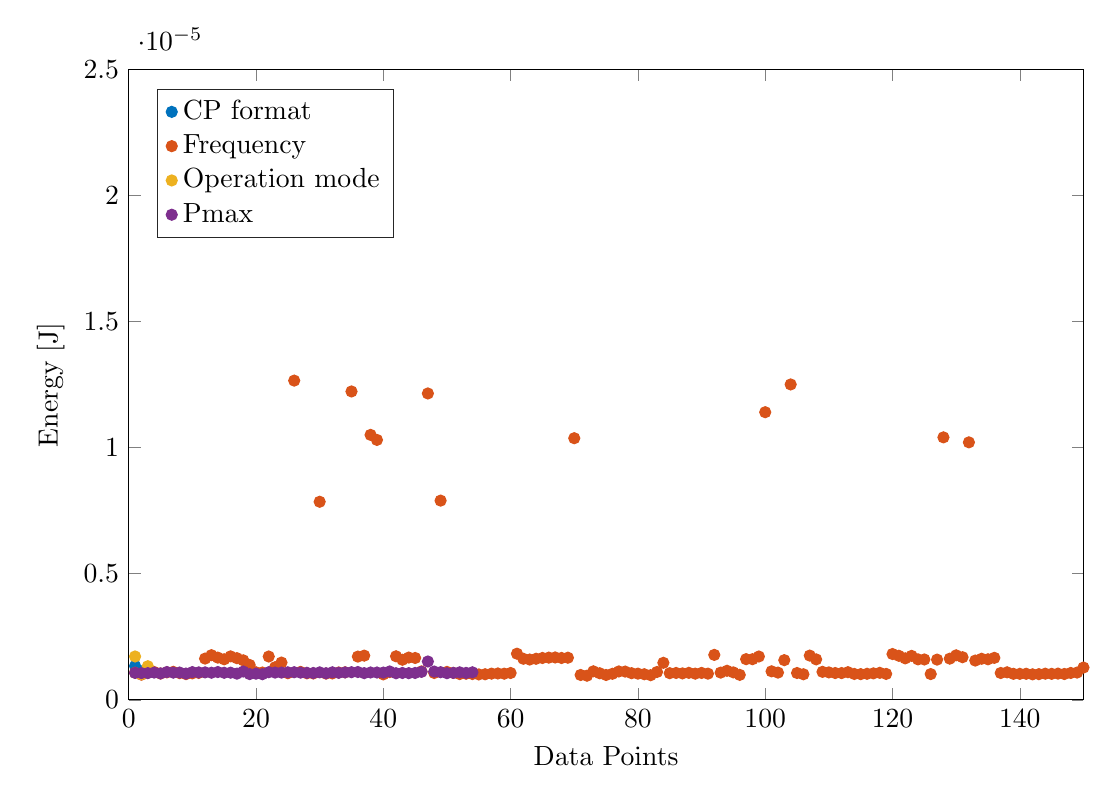
\begin{tikzpicture}

\begin{axis}[%
width=\textwidth,
height=0.66\textwidth,
at={(2.08in,0.858in)},
scale only axis,
xmin=0,
xmax=150,
xlabel={Data Points},
ymin=0,
ymax=2.5e-05,
ylabel={Energy [J]},
axis background/.style={fill=white},
%title style={font=\bfseries},
%title={Synchronization},
legend style={at={(0.03,0.97)},anchor=north west,legend cell align=left,align=right,draw=white!15!black}
]
\addplot [color=mycolor1,only marks,mark=*,mark options={solid}]
  table[row sep=crcr]{%
1	1.34067425208712e-06\\
2	1.12242602877281e-06\\
};
\addlegendentry{CP format};

\addplot [color=mycolor2,only marks,mark=*,mark options={solid}]
  table[row sep=crcr]{%
1	1.0756823088186e-06\\
2	9.97196253118895e-07\\
3	1.07530106959878e-06\\
4	1.10324330048733e-06\\
5	1.04014870921076e-06\\
6	1.08995478703403e-06\\
7	1.1088101599878e-06\\
8	1.0574919265968e-06\\
9	1.01933949858063e-06\\
10	1.0491033254808e-06\\
11	1.06707578286328e-06\\
12	1.63460769812375e-06\\
13	1.76965847945324e-06\\
14	1.6738210613843e-06\\
15	1.60690932864828e-06\\
16	1.72305997763063e-06\\
17	1.6508115391229e-06\\
18	1.56544019032926e-06\\
19	1.38199369240671e-06\\
20	1.09175487242403e-06\\
21	1.08166052595419e-06\\
22	1.71707936829757e-06\\
23	1.2924199967427e-06\\
24	1.47677538448511e-06\\
25	1.05464451047743e-06\\
26	1.26633908447658e-05\\
27	1.10713299878423e-06\\
28	1.05110069743594e-06\\
29	1.04509796344584e-06\\
30	7.85685380289262e-06\\
31	1.03941008462375e-06\\
32	1.04673374011435e-06\\
33	1.08389679662242e-06\\
34	1.08989320264378e-06\\
35	1.2232857822079e-05\\
36	1.71367546181616e-06\\
37	1.75188602710752e-06\\
38	1.05099817414129e-05\\
39	1.03102716006802e-05\\
40	1.00874506887433e-06\\
41	1.10039982398377e-06\\
42	1.72631780144864e-06\\
43	1.58841923592161e-06\\
44	1.67590984722733e-06\\
45	1.65918676629418e-06\\
46	1.12585857014324e-06\\
47	1.21532498016198e-05\\
48	1.0639670648209e-06\\
49	7.90220087917637e-06\\
50	1.10689124879218e-06\\
51	1.0676077696025e-06\\
52	1.02055968155225e-06\\
53	1.03395358962369e-06\\
54	1.02284176756657e-06\\
55	1.00698099365716e-06\\
56	1.01379266752505e-06\\
57	1.03784467029782e-06\\
58	1.04450143716487e-06\\
59	1.03554181243738e-06\\
60	1.06368443105705e-06\\
61	1.82842144943951e-06\\
62	1.62838648123534e-06\\
63	1.59678592550239e-06\\
64	1.62725781321621e-06\\
65	1.65902004362397e-06\\
66	1.67276848918022e-06\\
67	1.68009520248227e-06\\
68	1.65913762147219e-06\\
69	1.66958674466518e-06\\
70	1.03778659447381e-05\\
71	9.84603352986803e-07\\
72	9.56331062781806e-07\\
73	1.12956665075211e-06\\
74	1.05250931326862e-06\\
75	9.84810532273154e-07\\
76	1.03202459334288e-06\\
77	1.12447645031274e-06\\
78	1.1195701483476e-06\\
79	1.05549610825046e-06\\
80	1.03780730834437e-06\\
81	1.01451348392339e-06\\
82	9.7639080900736e-07\\
83	1.10388877159849e-06\\
84	1.46699178243079e-06\\
85	1.05528627769586e-06\\
86	1.06458895815028e-06\\
87	1.04739165217311e-06\\
88	1.06948595729843e-06\\
89	1.03704030611977e-06\\
90	1.06632948749806e-06\\
91	1.03752014683528e-06\\
92	1.78180333669874e-06\\
93	1.07831439734552e-06\\
94	1.15076575264746e-06\\
95	1.08720724352209e-06\\
96	9.88482488761432e-07\\
97	1.6120315796871e-06\\
98	1.6108189148589e-06\\
99	1.71780986353568e-06\\
100	1.14097621006086e-05\\
101	1.12966905992261e-06\\
102	1.07873402619562e-06\\
103	1.57303628227537e-06\\
104	1.25109337911685e-05\\
105	1.06306033639251e-06\\
106	1.01303664525916e-06\\
107	1.75385325235212e-06\\
108	1.60377716479687e-06\\
109	1.10900335278275e-06\\
110	1.08714248594812e-06\\
111	1.06173094639215e-06\\
112	1.06015971416799e-06\\
113	1.09544315069156e-06\\
114	1.02519762185331e-06\\
115	1.01783592260399e-06\\
116	1.0317569162224e-06\\
117	1.04889689721377e-06\\
118	1.06989439617546e-06\\
119	1.02707285658087e-06\\
120	1.81571982604701e-06\\
121	1.74532069170229e-06\\
122	1.64413315255404e-06\\
123	1.74222146043301e-06\\
124	1.60430704818907e-06\\
125	1.59930515569438e-06\\
126	1.02043187892461e-06\\
127	1.59417255244855e-06\\
128	1.04117727640757e-05\\
129	1.63276247008971e-06\\
130	1.76376031377767e-06\\
131	1.68926103201192e-06\\
132	1.02136090696712e-05\\
133	1.55646972188926e-06\\
134	1.62787210816775e-06\\
135	1.60662818064574e-06\\
136	1.66435120525633e-06\\
137	1.06309302326035e-06\\
138	1.09014975930545e-06\\
139	1.02966227181924e-06\\
140	1.0298157208698e-06\\
141	1.03261820054816e-06\\
142	1.01021929908402e-06\\
143	1.01759878321502e-06\\
144	1.03589330412151e-06\\
145	1.02904015412003e-06\\
146	1.0388339664431e-06\\
147	1.02325681731463e-06\\
148	1.06454234831571e-06\\
149	1.08137970610969e-06\\
150	1.2792154864867e-06\\
};
\addlegendentry{Frequency};

\addplot [color=mycolor3,only marks,mark=*,mark options={solid}]
  table[row sep=crcr]{%
1	1.71863070186303e-06\\
2	1.01456363868033e-06\\
3	1.33120240444451e-06\\
};
\addlegendentry{Operation mode};

\addplot [color=mycolor4,only marks,mark=*,mark options={solid}]
  table[row sep=crcr]{%
1	1.0671797625832e-06\\
2	1.0588456898191e-06\\
3	1.05795589484699e-06\\
4	1.08055848780402e-06\\
5	1.04762808644952e-06\\
6	1.1013140820616e-06\\
7	1.07759871557913e-06\\
8	1.08160697361213e-06\\
9	1.04025231904184e-06\\
10	1.09816496570356e-06\\
11	1.08714269056602e-06\\
12	1.08761153797267e-06\\
13	1.07365285652857e-06\\
14	1.10125425405216e-06\\
15	1.07156572489788e-06\\
16	1.0759174643657e-06\\
17	1.03783488430604e-06\\
18	1.12183899012571e-06\\
19	1.0201216620912e-06\\
20	1.03660357243892e-06\\
21	1.01556518712642e-06\\
22	1.09429710451097e-06\\
23	1.0796650157043e-06\\
24	1.07937842520173e-06\\
25	1.08979312304457e-06\\
26	1.09333904615246e-06\\
27	1.07734439096524e-06\\
28	1.07069784829799e-06\\
29	1.06280968742978e-06\\
30	1.08881266457677e-06\\
31	1.05410891640532e-06\\
32	1.09146145961626e-06\\
33	1.07078720758496e-06\\
34	1.08727910212997e-06\\
35	1.09437331228688e-06\\
36	1.10180616008859e-06\\
37	1.05744390923426e-06\\
38	1.08339901023109e-06\\
39	1.08311458846742e-06\\
40	1.07909301411026e-06\\
41	1.12340040319467e-06\\
42	1.05293692062927e-06\\
43	1.06402922366403e-06\\
44	1.05680910463732e-06\\
45	1.06535147640935e-06\\
46	1.10944323021434e-06\\
47	1.51935088635014e-06\\
48	1.12051665665269e-06\\
49	1.09551654623524e-06\\
50	1.05557387096436e-06\\
51	1.06804892364889e-06\\
52	1.09046565872179e-06\\
53	1.06742440177378e-06\\
54	1.0907300220633e-06\\
};
\addlegendentry{Pmax};

\end{axis}
\end{tikzpicture}%}
\end{minipage}
\hfill
\begin{minipage}{0.48\textwidth}
\tikzsetnextfilename{Sync_Stat}
\resizebox{\textwidth}{!}{
% This file was created by matlab2tikz.
%
%The latest updates can be retrieved from
%  http://www.mathworks.com/matlabcentral/fileexchange/22022-matlab2tikz-matlab2tikz
%where you can also make suggestions and rate matlab2tikz.
%
%Point distribution 
%mean = -1.324114754962850 
%var = 0.377191701414210
%
\definecolor{mycolor1}{rgb}{0.00000,0.44700,0.74100}%
\definecolor{mycolor2}{rgb}{0.85000,0.32500,0.09800}%
%
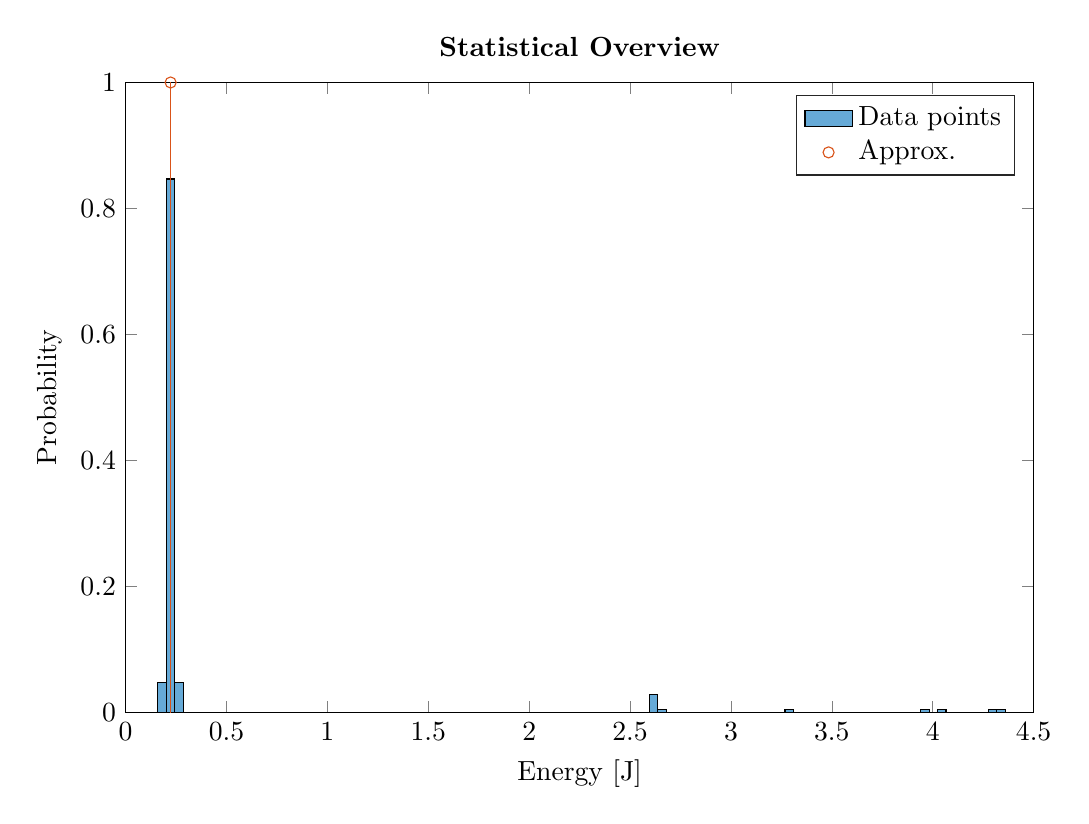
\begin{tikzpicture}

\begin{axis}[%
width=0.951\textwidth,
height=0.66\textwidth,
at={(0\textwidth,0\textwidth)},
scale only axis,
xmin=0,
xmax=4.5,
xlabel={Energy [J]},
ymin=0,
ymax=1,
ylabel={Probability},
axis background/.style={fill=white},
title style={font=\bfseries},
title={Statistical Overview},
legend style={legend cell align=left,align=left,draw=white!15!black},
y tick label style={/pgf/number format/fixed}
]
\addplot[fill=mycolor1,fill opacity=0.6,draw=black,ybar interval,area legend] plot table[row sep=crcr] {%
x	y\\
0.16	0.0478468899521531\\
0.202	0.84688995215311\\
0.244	0.0478468899521531\\
0.286	0\\
0.328	0\\
0.37	0\\
0.412	0\\
0.454	0\\
0.496	0\\
0.538	0\\
0.58	0\\
0.622	0\\
0.664	0\\
0.706	0\\
0.748	0\\
0.79	0\\
0.832	0\\
0.874	0\\
0.916	0\\
0.958	0\\
1	0\\
1.042	0\\
1.084	0\\
1.126	0\\
1.168	0\\
1.21	0\\
1.252	0\\
1.294	0\\
1.336	0\\
1.378	0\\
1.42	0\\
1.462	0\\
1.504	0\\
1.546	0\\
1.588	0\\
1.63	0\\
1.672	0\\
1.714	0\\
1.756	0\\
1.798	0\\
1.84	0\\
1.882	0\\
1.924	0\\
1.966	0\\
2.008	0\\
2.05	0\\
2.092	0\\
2.134	0\\
2.176	0\\
2.218	0\\
2.26	0\\
2.302	0\\
2.344	0\\
2.386	0\\
2.428	0\\
2.47	0\\
2.512	0\\
2.554	0\\
2.596	0.0287081339712919\\
2.638	0.00478468899521531\\
2.68	0\\
2.722	0\\
2.764	0\\
2.806	0\\
2.848	0\\
2.89	0\\
2.932	0\\
2.974	0\\
3.016	0\\
3.058	0\\
3.1	0\\
3.142	0\\
3.184	0\\
3.226	0\\
3.268	0.00478468899521531\\
3.31	0\\
3.352	0\\
3.394	0\\
3.436	0\\
3.478	0\\
3.52	0\\
3.562	0\\
3.604	0\\
3.646	0\\
3.688	0\\
3.73	0\\
3.772	0\\
3.814	0\\
3.856	0\\
3.898	0\\
3.94	0.00478468899521531\\
3.982	0\\
4.024	0.00478468899521531\\
4.066	0\\
4.108	0\\
4.15	0\\
4.192	0\\
4.234	0\\
4.276	0.00478468899521531\\
4.318	0.00478468899521531\\
4.36	0.00478468899521531\\
};
\addlegendentry{Data points};

\addplot[ycomb,color=mycolor2,solid,mark=o,mark options={solid}] plot table[row sep=crcr] 
\end{minipage}
\caption{Energy consumed during boot up and cell synchronization.}
\label{fig:Sync_Points}
\end{figure}

As it can be seen in \autoref{fig:Sync_Points} all of the considered parameters is without characteristic influence. It can be seen though that a few points is a little higher than the rest, but looking at it statistically they can be neglected, this is also expected as seen in \autoref{sec:bat_model}. A single point is therefore chosen as it is assumed the small discrepancies around it is due to the small difference in synchronization time, that might arise depending on where in the \gls{SIB} messages the device gets active. 

The next element to look at is the energy used to attach to the network. This is found based on the log where a messages is telling where the NPRACH starts and where the attach is complete. This can be seen as area B in \autoref{fig:Attach_raw}. It is determined to split the energy into the average power and the time it takes based on the measurements. First the power is found based on \autoref{eq:power} for area B. 
This is done for all measurements and the results are presented in \autoref{fig:Attach_Power_Points}.

\begin{figure}[H]
\centering
\begin{minipage}{0.48\textwidth}
\tikzsetnextfilename{Attach_Power_Points}
\resizebox{\textwidth}{!}{
% This file was created by matlab2tikz.
%
%The latest updates can be retrieved from
%  http://www.mathworks.com/matlabcentral/fileexchange/22022-matlab2tikz-matlab2tikz
%where you can also make suggestions and rate matlab2tikz.
%
\definecolor{mycolor1}{rgb}{0.00000,0.44700,0.74100}%
\definecolor{mycolor2}{rgb}{0.85000,0.32500,0.09800}%
\definecolor{mycolor3}{rgb}{0.92900,0.69400,0.12500}%
%
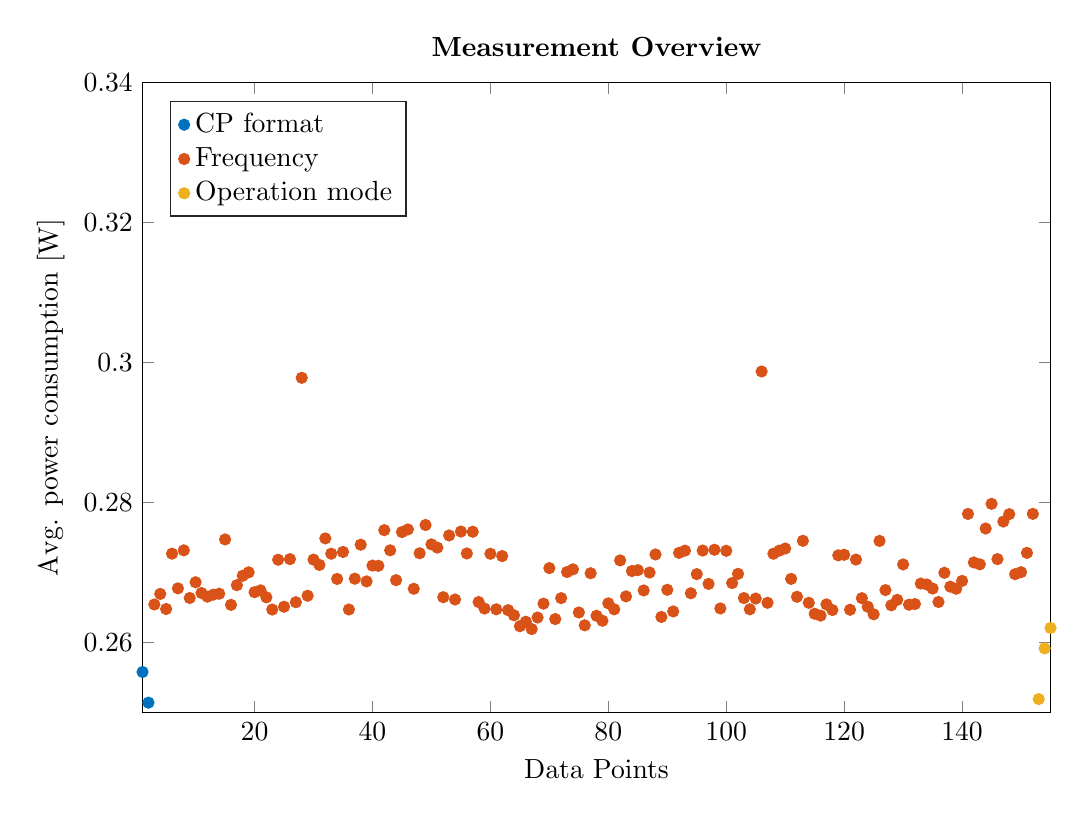
\begin{tikzpicture}

\begin{axis}[%
width=0.951\textwidth,
height=0.66\textwidth,
at={(0\textwidth,0\textwidth)},
scale only axis,
xmin=1,
xmax=155,
xlabel={Data Points},
ymin=0.25,
ymax=0.34,
ylabel={Avg. power consumption [W]},
axis background/.style={fill=white},
title style={font=\bfseries},
title={Measurement Overview},
legend style={at={(0.03,0.97)},anchor=north west,legend cell align=left,align=left,draw=white!15!black},
y tick label style={/pgf/number format/fixed}
]
\addplot [color=mycolor1,only marks,mark=*,mark options={solid}]
  table[row sep=crcr]{%
1	0.255801781387079\\
2	0.251421193899255\\
};
\addlegendentry{CP format};

\addplot [color=mycolor2,only marks,mark=*,mark options={solid}]
  table[row sep=crcr]{%
3	0.265445452572333\\
4	0.266954209300766\\
5	0.264797928614294\\
6	0.272704083459804\\
7	0.267746363195588\\
8	0.273178340361388\\
9	0.266368901171886\\
10	0.268619684665784\\
11	0.26708039540221\\
12	0.26655998303708\\
13	0.266845320410119\\
14	0.26698328534778\\
15	0.274736472721134\\
16	0.26539051637896\\
17	0.26820485827082\\
18	0.269552843355458\\
19	0.270038646899647\\
20	0.267200278116755\\
21	0.267458859897132\\
22	0.266468679143444\\
23	0.26471865694658\\
24	0.271832738092186\\
25	0.265124819513339\\
26	0.271922464341057\\
27	0.26576713342322\\
28	0.297821655391698\\
29	0.266692748192563\\
30	0.27185355957331\\
31	0.27109167349431\\
32	0.274880327160046\\
33	0.272695441318171\\
34	0.269091895735741\\
35	0.272947558238\\
36	0.264727815075479\\
37	0.269121646325412\\
38	0.273982228971079\\
39	0.268740328073609\\
40	0.271002884242907\\
41	0.270969670950985\\
42	0.276056888833248\\
43	0.273177349384088\\
44	0.26891830134814\\
45	0.275789507233496\\
46	0.276163342958147\\
47	0.267687699991572\\
48	0.27275713803948\\
49	0.276798360841021\\
50	0.274031090363989\\
51	0.273568020346507\\
52	0.266483755723602\\
53	0.275306897683914\\
54	0.266156483990352\\
55	0.275860617369944\\
56	0.272732960453597\\
57	0.275832360931848\\
58	0.265790729613348\\
59	0.264866706743245\\
60	0.27268646654511\\
61	0.264753886733427\\
62	0.272355979523188\\
63	0.264634276307107\\
64	0.263899661419284\\
65	0.262340020610494\\
66	0.262979411732452\\
67	0.261931117679891\\
68	0.26357937047217\\
69	0.26556369307208\\
70	0.270640483343679\\
71	0.263361875135284\\
72	0.266352652929479\\
73	0.270079331364635\\
74	0.270463024741068\\
75	0.264301440365561\\
76	0.262465009871972\\
77	0.269909229745724\\
78	0.263830255992203\\
79	0.26312089127998\\
80	0.265610113533262\\
81	0.264752943169823\\
82	0.271741014345849\\
83	0.266602782621202\\
84	0.270223435545716\\
85	0.270346941149791\\
86	0.267448254432004\\
87	0.27000486018762\\
88	0.272588367329993\\
89	0.263662673885227\\
90	0.267540780880364\\
91	0.264446563400098\\
92	0.272814771249928\\
93	0.273135136900738\\
94	0.267048611657137\\
95	0.269776935214174\\
96	0.273145441050165\\
97	0.268382709252621\\
98	0.27325746904602\\
99	0.264877676225099\\
100	0.273111618218773\\
101	0.268504508185846\\
102	0.26981930830676\\
103	0.26635946567318\\
104	0.26475272191475\\
105	0.266291505024782\\
106	0.298721808531873\\
107	0.265683446153979\\
108	0.272693837948645\\
109	0.273133025449803\\
110	0.27343760359363\\
111	0.269099368354071\\
112	0.266543572066331\\
113	0.274539036010476\\
114	0.265681406612183\\
115	0.264117585450568\\
116	0.2638563551989\\
117	0.265457769724398\\
118	0.264650225933215\\
119	0.272462026303984\\
120	0.272541196122011\\
121	0.264688911717546\\
122	0.27185822484575\\
123	0.266344679318229\\
124	0.265120973142423\\
125	0.264044325882864\\
126	0.274519937915519\\
127	0.267497846746046\\
128	0.26532517894989\\
129	0.266108968347231\\
130	0.271165338108506\\
131	0.26541109379603\\
132	0.265506580313867\\
133	0.268428618015063\\
134	0.268303887513969\\
135	0.267725430056234\\
136	0.265800497472174\\
137	0.269969688927248\\
138	0.267988154047674\\
139	0.267691948327441\\
140	0.268813192576425\\
141	0.278376814778973\\
142	0.271446959287438\\
143	0.271177312223487\\
144	0.276294566737266\\
145	0.279817661513477\\
146	0.271924769209123\\
147	0.27728984238318\\
148	0.278348619230541\\
149	0.26977093324355\\
150	0.270057690768147\\
151	0.272815459477205\\
152	0.27838604219041\\
};
\addlegendentry{Frequency};

\addplot [color=mycolor3,only marks,mark=*,mark options={solid}]
  table[row sep=crcr]
\end{minipage}
\hfill
\begin{minipage}{0.48\textwidth}
\tikzsetnextfilename{Attach_Power_Stat}
\resizebox{\textwidth}{!}{
% This file was created by matlab2tikz.
%
%The latest updates can be retrieved from
%  http://www.mathworks.com/matlabcentral/fileexchange/22022-matlab2tikz-matlab2tikz
%where you can also make suggestions and rate matlab2tikz.
%
\definecolor{mycolor1}{rgb}{0.00000,0.44700,0.74100}%
\definecolor{mycolor2}{rgb}{0.85000,0.32500,0.09800}%
%
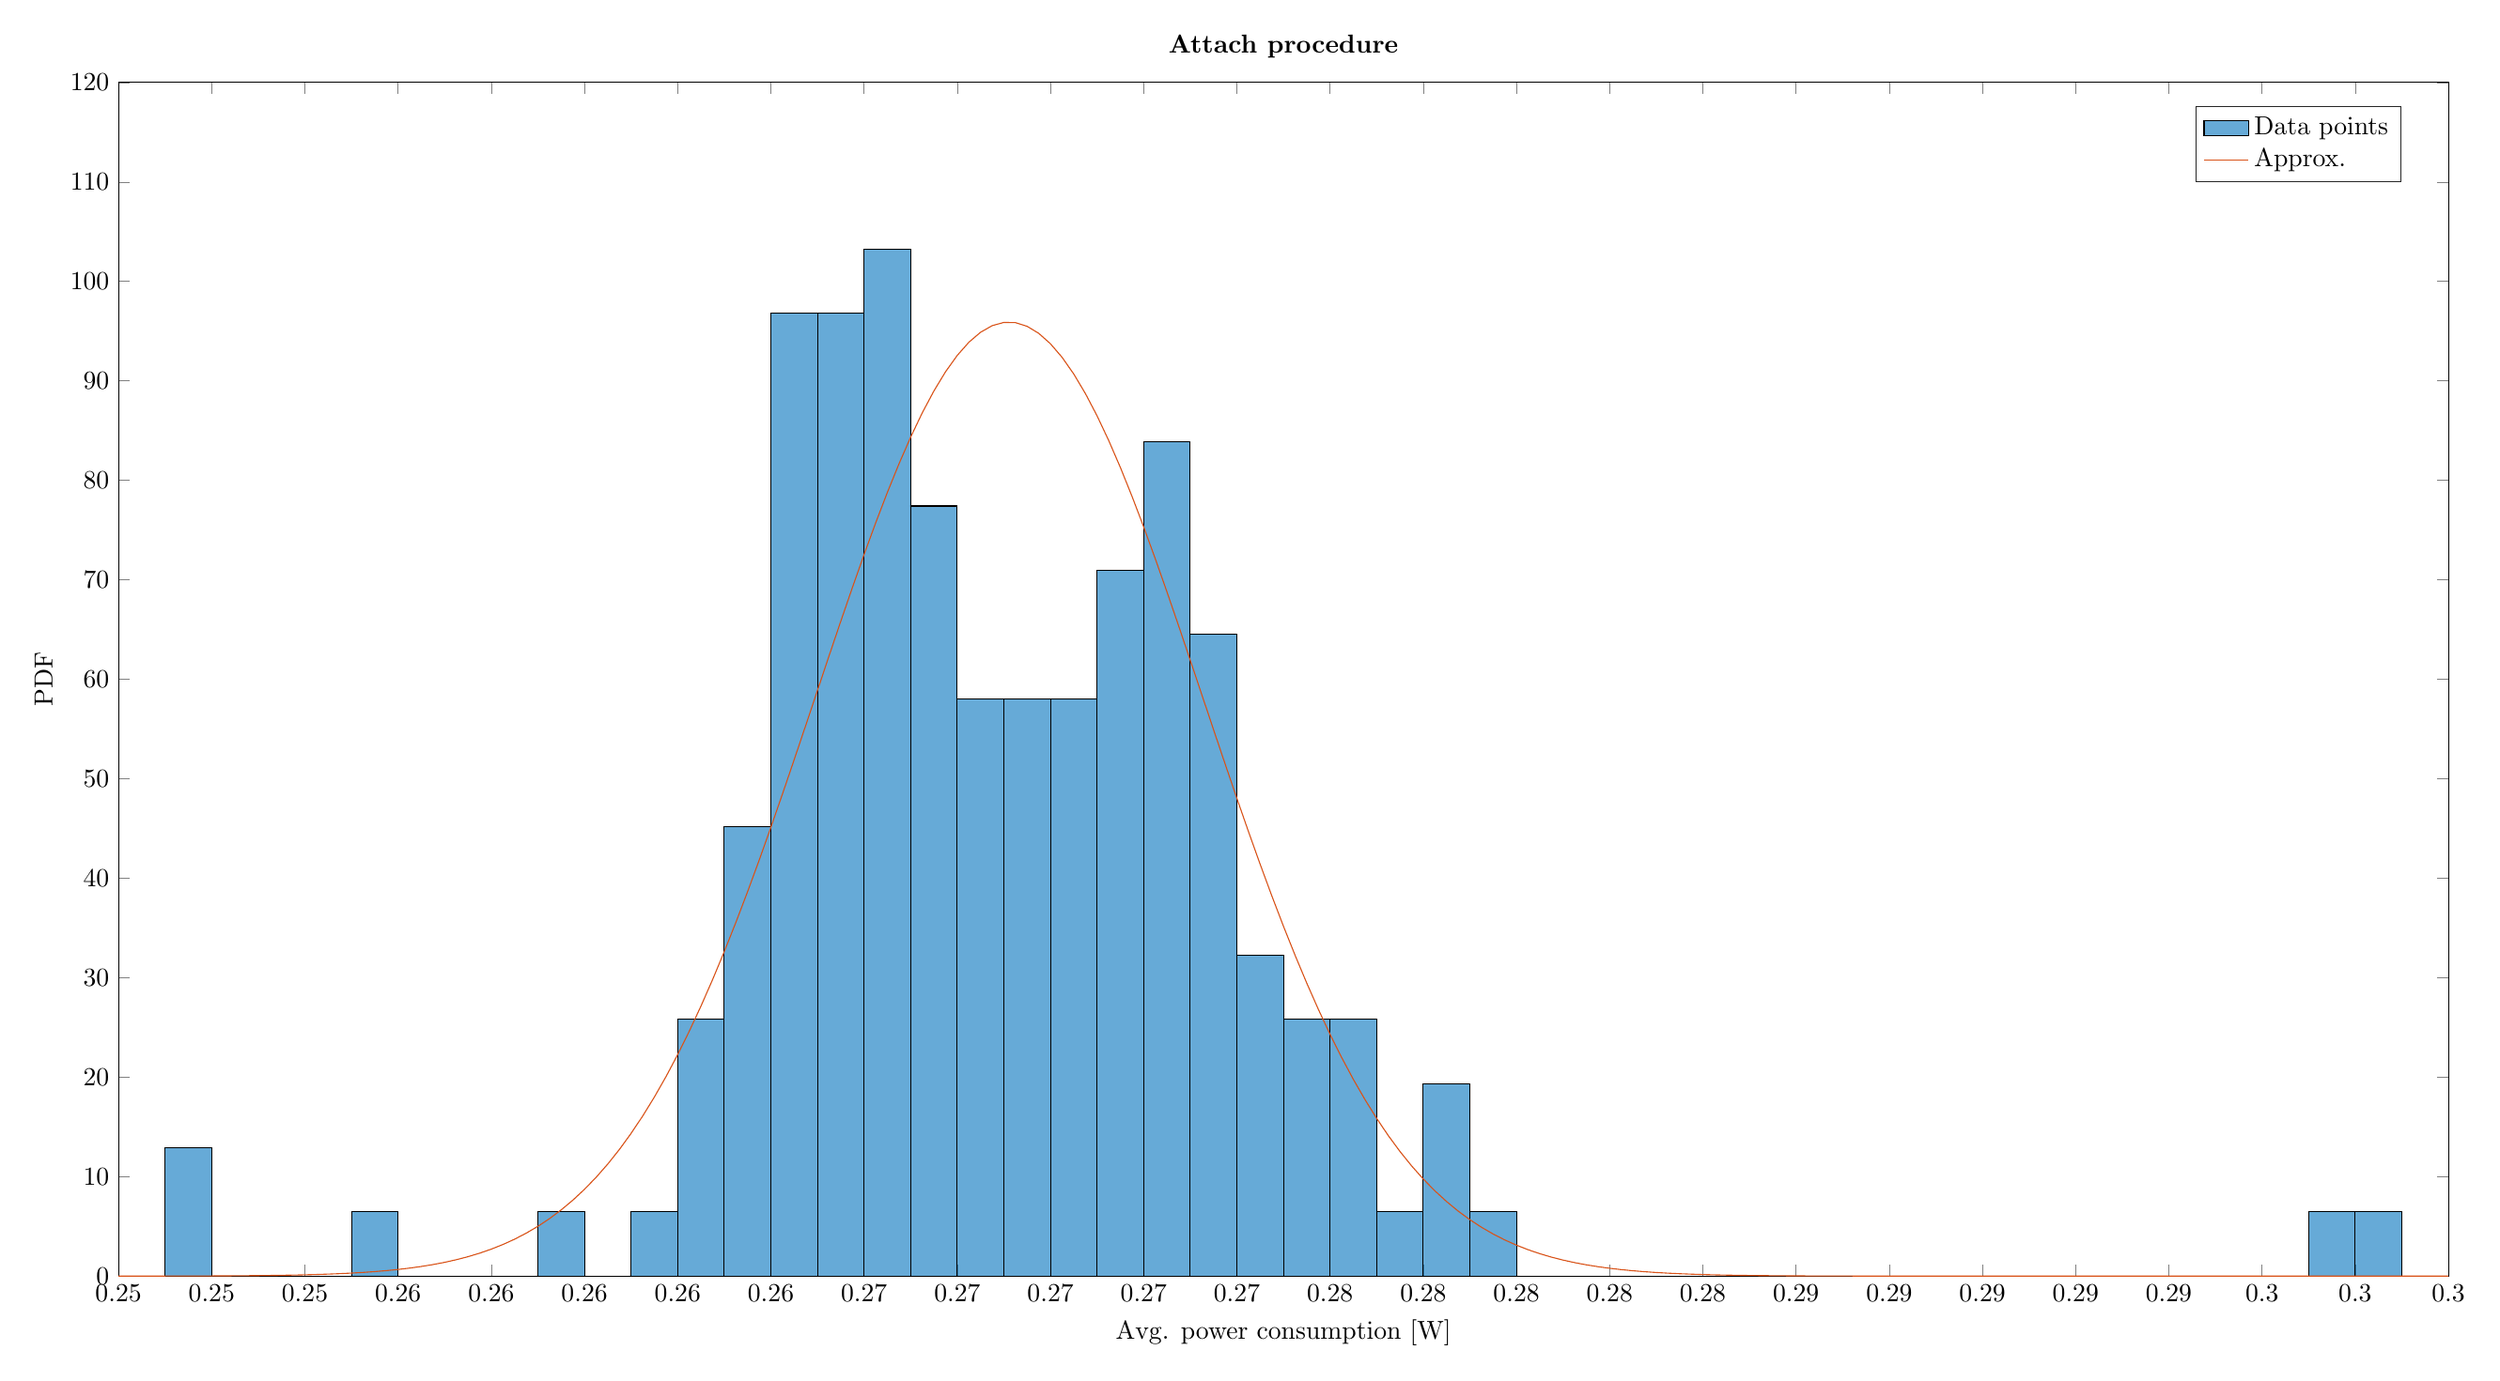
\begin{tikzpicture}

\begin{axis}[%
width=12.4in,
height=6.357in,
at={(2.08in,0.858in)},
scale only axis,
xmin=0.25,
xmax=0.3,
xlabel={Avg. power consumption [W]},
ymin=0,
ymax=120,
ylabel={PDF},
axis background/.style={fill=white},
title style={font=\bfseries},
title={Attach procedure},
legend style={legend cell align=left,align=left,draw=white!15!black}
]
\addplot[fill=mycolor1,fill opacity=0.6,draw=black,ybar interval,area legend] plot table[row sep=crcr] {%
x	y\\
0.251	12.9032258064516\\
0.252	0\\
0.253	0\\
0.254	0\\
0.255	6.4516129032258\\
0.256	0\\
0.257	0\\
0.258	0\\
0.259	6.4516129032258\\
0.26	0\\
0.261	6.4516129032258\\
0.262	25.8064516129032\\
0.263	45.1612903225806\\
0.264	96.774193548387\\
0.265	96.774193548387\\
0.266	103.225806451613\\
0.267	77.4193548387096\\
0.268	58.0645161290322\\
0.269	58.0645161290322\\
0.27	58.0645161290322\\
0.271	70.9677419354838\\
0.272	83.8709677419354\\
0.273	64.516129032258\\
0.274	32.258064516129\\
0.275	25.8064516129032\\
0.276	25.8064516129032\\
0.277	6.4516129032258\\
0.278	19.3548387096774\\
0.279	6.4516129032258\\
0.28	0\\
0.281	0\\
0.282	0\\
0.283	0\\
0.284	0\\
0.285	0\\
0.286	0\\
0.287	0\\
0.288	0\\
0.289	0\\
0.29	0\\
0.291	0\\
0.292	0\\
0.293	0\\
0.294	0\\
0.295	0\\
0.296	0\\
0.297	6.4516129032258\\
0.298	6.4516129032258\\
0.299	6.4516129032258\\
};
\addlegendentry{Data points};

\addplot [color=mycolor2,solid]
  table[row sep=crcr]{%
0.25	0.00250657473119294\\
0.25025	0.0032976865354245\\
0.2505	0.00432284099601417\\
0.25075	0.00564625292597716\\
0.251	0.0073482271433148\\
0.25125	0.00952875132032203\\
0.2515	0.0123117727336095\\
0.25175	0.0158502590302116\\
0.252	0.0203321504445364\\
0.25225	0.0259873168600061\\
0.2525	0.0330956370892701\\
0.25275	0.0419963190295325\\
0.253	0.0530985771213465\\
0.25325	0.0668937768999349\\
0.2535	0.0839691444080249\\
0.25375	0.105023119821819\\
0.254	0.130882408798454\\
0.25425	0.162520750783369\\
0.2545	0.201079379901437\\
0.25475	0.247889100319376\\
0.255	0.304493833547149\\
0.25525	0.372675419768861\\
0.2555	0.454479369062153\\
0.25575	0.552241161835877\\
0.256	0.668612592091787\\
0.25625	0.806587533909809\\
0.2565	0.969526393269745\\
0.25675	1.16117838707287\\
0.257	1.38570067289165\\
0.25725	1.647673241155\\
0.2575	1.95210838147723\\
0.25775	2.30445345255048\\
0.258	2.71058562681963\\
0.25825	3.17679725367845\\
0.2585	3.70977049487734\\
0.25875	4.31653993966137\\
0.259	5.00444201079945\\
0.25925	5.78105013110826\\
0.2595	6.65409483708686\\
0.25975	7.63136830392007\\
0.26	8.72061308450107\\
0.26025	9.9293952619723\\
0.2605	11.2649626657786\\
0.26075	12.7340892976578\\
0.261	14.3429076458791\\
0.26125	16.0967311199051\\
0.2615	17.9998693974747\\
0.26175	20.0554400233162\\
0.262	22.2651801129792\\
0.26225	24.6292624748067\\
0.2625	27.1461208456691\\
0.26275	29.8122892196452\\
0.263	32.6222604127393\\
0.26325	35.5683690323456\\
0.2635	38.6407038924218\\
0.26375	41.8270546230625\\
0.264	45.1128967606433\\
0.26425	48.481418971733\\
0.2645	51.9135952670472\\
0.26475	55.3883041136952\\
0.265	58.8824952747747\\
0.26525	62.3714040209691\\
0.2655	65.8288111014464\\
0.26575	69.2273455678449\\
0.266	72.5388262564806\\
0.26625	75.734636493136\\
0.2665	78.7861254360654\\
0.26675	81.6650284590181\\
0.267	84.3438981375949\\
0.26725	86.7965367746851\\
0.2675	88.9984210138402\\
0.26775	90.9271089650223\\
0.268	92.5626204185446\\
0.26825	93.8877811535896\\
0.2685	94.8885230510621\\
0.26875	95.5541326799721\\
0.269	95.877442215908\\
0.26925	95.8549579343015\\
0.2695	95.4869230575807\\
0.26975	94.777313375367\\
0.27	93.7337657479967\\
0.27025	92.3674412912183\\
0.2705	90.6928266694099\\
0.27075	88.7274784439277\\
0.271	86.491716784298\\
0.27125	84.0082760112857\\
0.2715	81.3019203683351\\
0.27175	78.3990340865621\\
0.272	75.327195202932\\
0.27225	72.114742706425\\
0.2725	68.7903464275379\\
0.27275	65.3825886669198\\
0.273	61.9195659021577\\
0.27325	58.4285180483469\\
0.2735	54.9354917143696\\
0.27375	51.4650427336713\\
0.274	48.0399819988332\\
0.27425	44.6811673375642\\
0.2745	41.4073428766698\\
0.27475	38.2350260906836\\
0.275	35.1784415594125\\
0.27525	32.2494993951381\\
0.2755	29.4578153708413\\
0.27575	26.810769004589\\
0.276	24.3135952441767\\
0.27625	21.9695049558088\\
0.2765	19.7798291501919\\
0.27675	17.7441817722427\\
0.277	15.8606359251921\\
0.27725	14.1259085803524\\
0.2775	12.5355491215027\\
0.27775	11.0841274666452\\
0.278	9.76541797782621\\
0.27825	8.57257588943834\\
0.2785	7.49830353542448\\
0.27875	6.53500421581358\\
0.279	5.67492209491789\\
0.27925	4.91026705147031\\
0.2795	4.23332389200655\\
0.27975	3.63654578267462\\
0.28	3.11263214414857\\
0.28025	2.65459158488421\\
0.2805	2.25579071768812\\
0.28075	1.90998991380775\\
0.281	1.61136719984676\\
0.28125	1.35453159966702\\
0.2815	1.13452727122929\\
0.28175	0.946829793034706\\
0.282	0.787335922986492\\
0.28225	0.652348090785433\\
0.2825	0.538554800038131\\
0.28275	0.443008014396615\\
0.283	0.363098489099697\\
0.28325	0.296529890454474\\
0.2835	0.241292425601816\\
0.28375	0.195636587119796\\
0.284	0.158047504665887\\
0.28425	0.12722029124399\\
0.2845	0.102036676441757\\
0.28475	0.0815431341396076\\
0.285	0.0649306382424204\\
0.28525	0.0515161169740215\\
0.2855	0.0407256238902799\\
0.28575	0.0320792014125493\\
0.286	0.0251773795621062\\
0.28625	0.0196892277545122\\
0.2865	0.0153418599846826\\
0.28675	0.0119112824685886\\
0.287	0.0092144667947042\\
0.28725	0.00710252991502466\\
0.2875	0.00545490398251483\\
0.28775	0.00417438331725745\\
0.288	0.00318294195221813\\
0.28825	0.00241822266525369\\
0.2885	0.00183060663869301\\
0.28875	0.00138078148624045\\
0.289	0.00103773401971343\\
0.28925	0.000777102542695656\\
0.2895	0.000579831469477415\\
0.28975	0.0004310785480119\\
0.29	0.000319331835339855\\
0.29025	0.000235699792107263\\
0.2905	0.000173343419104506\\
0.29075	0.000127024266066903\\
0.291	9.27464310637832e-05\\
0.29125	6.74743789362491e-05\\
0.2915	4.89115878215108e-05\\
0.29175	3.53277358178498e-05\\
0.292	2.54244181806689e-05\\
0.29225	1.82312908266504e-05\\
0.2925	1.30261175051744e-05\\
0.29275	9.27350137483121e-06\\
0.293	6.57814839701643e-06\\
0.29325	4.64937706644976e-06\\
0.2935	3.27428929553815e-06\\
0.29375	2.29757927022029e-06\\
0.294	1.60640533114901e-06\\
0.29425	1.11910528317453e-06\\
0.2945	7.76815588277944e-07\\
0.29475	5.37274334058155e-07\\
0.295	3.70258837989432e-07\\
0.29525	2.5424121175473e-07\\
0.2955	1.73947280128578e-07\\
0.29575	1.18582475340827e-07\\
0.296	8.05479622306248e-08\\
0.29625	5.45154724808003e-08\\
0.2965	3.67634431919681e-08\\
0.29675	2.47026619855903e-08\\
0.297	1.6538743377329e-08\\
0.29725	1.10329700166221e-08\\
0.2975	7.33353795457553e-09\\
0.29775	4.85697453808339e-09\\
0.298	3.20515684150475e-09\\
0.29825	2.10748223435791e-09\\
0.2985	1.38073309640352e-09\\
0.29875	9.01336014757792e-10\\
0.299	5.86266246125221e-10\\
0.29925	3.79956810619947e-10\\
0.2995	2.45360559342778e-10\\
0.29975	1.57872486509382e-10\\
0.3	1.01213704827537e-10\\
};
\addlegendentry{Approx.};

\end{axis}
\end{tikzpicture}%}
\end{minipage}
\caption{Average power consumption during attach procedure.}
\label{fig:Attach_Power_Points}
\end{figure}

As seen from \autoref{fig:Attach_Power_Points} the $P_{TX}$ has a significant effect on the average power consumption and is will therefore be investigated separately. It looks like almost all frequency measurements is a layer above the others, this is unexpected as a common point shared across all four parameters, which should therefore have used the same average power. It might also look like CP-format and operation mode has an influence on the average power consumption, but comparing to the spread of the frequency it is neglectable. The variance is investigated statistically, a lognormal distribution is chosen to approximate the power consumption as it is assumed, that the fluctuation of the current should be normal distributed and since the power is the current squared and therefore always positive it would should have a lognormal behaviour.  

As mentioned the parameter $P_{TX}$ influences the mean value of the power consumption during the attach procedure, this can be seen in \autoref{fig:Attach_Pmax}. 

\begin{figure}[H]
\centering
\tikzsetnextfilename{Attach_Pmax}
\resizebox{0.7\textwidth}{!}{
% This file was created by matlab2tikz.
%
%The latest updates can be retrieved from
%  http://www.mathworks.com/matlabcentral/fileexchange/22022-matlab2tikz-matlab2tikz
%where you can also make suggestions and rate matlab2tikz.
%
\definecolor{mycolor1}{rgb}{0.00000,0.44700,0.74100}%
\definecolor{mycolor2}{rgb}{0.85000,0.32500,0.09800}%
\definecolor{mycolor3}{rgb}{0.92900,0.69400,0.12500}%
%
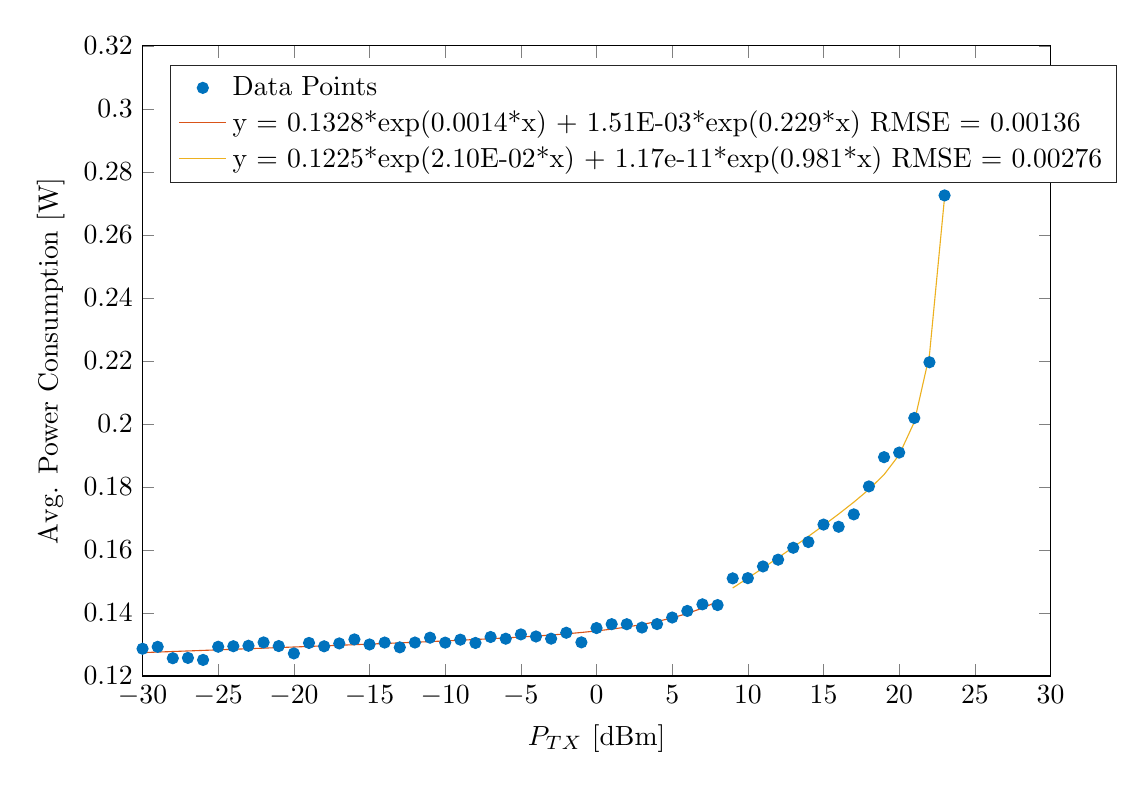
\begin{tikzpicture}

\begin{axis}[%
width=0.951\textwidth,
height=0.66\textwidth,
at={(0\textwidth,0\textwidth)},
scale only axis,
xmin=-30,
xmax=30,
xlabel={$P_{TX}$ [dBm]},
ymin=0.12,
ymax=0.32,
ylabel={Avg. Power Consumption [W]},
axis background/.style={fill=white},
legend style={at={(0.03,0.97)},anchor=north west,legend cell align=left,align=left,draw=white!15!black},
y tick label style={/pgf/number format/fixed}
]
\addplot [color=mycolor1,only marks,mark=*,mark options={solid}]
  table[row sep=crcr]{%
10	0.151047313371487\\
11	0.154761231210888\\
12	0.156907209211033\\
13	0.160684296068248\\
14	0.162507067874023\\
15	0.168046628044659\\
16	0.167349824554413\\
17	0.171283150343803\\
18	0.180161933269978\\
19	0.189439361249306\\
20	0.190898508743685\\
21	0.201872122219901\\
22	0.219567639872928\\
23	0.272516970950456\\
9	0.150974118861972\\
-1	0.130660121937841\\
-10	0.130575324810667\\
-11	0.132150467709027\\
-12	0.130605932962615\\
-13	0.129078875349553\\
-14	0.130599994705029\\
-15	0.129996957966701\\
-16	0.131599561535464\\
-17	0.130325487903084\\
-18	0.129413615846293\\
-19	0.13048045065209\\
-2	0.133708928603574\\
-20	0.127151660592556\\
-21	0.129485852333684\\
-22	0.13064634706093\\
-23	0.129580782637227\\
-24	0.129435597322756\\
-25	0.129270377248005\\
-26	0.125087904466061\\
-27	0.125727964840569\\
-28	0.125627487672513\\
-29	0.12924531898976\\
-3	0.131838548678704\\
-30	0.12863679811696\\
-4	0.132531210544604\\
-5	0.133192324600549\\
-6	0.131820841838912\\
-7	0.132364387132469\\
-8	0.130477571591827\\
-9	0.13151969584952\\
0	0.135203216563572\\
1	0.136439430941167\\
2	0.136422353003321\\
3	0.135367589970859\\
4	0.136472125157741\\
5	0.138547714791761\\
6	0.140637304886408\\
7	0.14273115545425\\
8	0.142493961491374\\
};
\addlegendentry{Data Points};

\addplot [color=mycolor2,solid]
  table[row sep=crcr]{%
-30	0.127404890355152\\
-29	0.127581064519652\\
-28	0.127757585925784\\
-27	0.127934481801407\\
-26	0.128111786279127\\
-25	0.128289542168819\\
-24	0.128467803185214\\
-23	0.128646636747371\\
-22	0.128826127496846\\
-21	0.129006381719082\\
-20	0.129187532899891\\
-19	0.12936974870845\\
-18	0.129553239773022\\
-17	0.129738270709663\\
-16	0.129925173982303\\
-15	0.130114367321117\\
-14	0.130306375612679\\
-13	0.130501858409943\\
-12	0.130701644504829\\
-11	0.130906775376563\\
-10	0.131118559794461\\
-9	0.13133864243879\\
-8	0.131569090138571\\
-7	0.131812500249081\\
-6	0.132072136852947\\
-5	0.13235210192795\\
-4	0.132657550458482\\
-3	0.132994960772249\\
-2	0.13337247428011\\
-1	0.133800322436827\\
0	0.134291363314813\\
1	0.134861755931651\\
2	0.135531807696734\\
3	0.136327039421605\\
4	0.137279523748831\\
5	0.13842956719373\\
6	0.139827824014172\\
7	0.141537952771039\\
8	0.143639954903506\\
};
\addlegendentry{y = 0.1328*exp(0.0014*x) + 1.51E-03*exp(0.229*x) RMSE = 0.00136};

\addplot [color=mycolor3,solid]
  table[row sep=crcr]
\caption{Average power consumption as a function of $P_{TX}$ during the attach procedure.}
\label{fig:Attach_Pmax}
\end{figure}

From \autoref{fig:Attach_Pmax} it can be seen that the power consumption can be approximated using two functions based on the value of $P_{TX}$. The need for two function to approximate the characteristic can be contributed to the usage of a power amplifier. This parameter determines the mean value of the average power consumption. 

Now the time to attach is investigated the time is found based on \autoref{eq:time} and the results can be seen in \autoref{fig:Attach_Time_Points}.


\begin{figure}[H]
\centering
\begin{minipage}{0.48\textwidth}
\tikzsetnextfilename{Attach_Time_Points}
\resizebox{\textwidth}{!}{
% This file was created by matlab2tikz.
%
%The latest updates can be retrieved from
%  http://www.mathworks.com/matlabcentral/fileexchange/22022-matlab2tikz-matlab2tikz
%where you can also make suggestions and rate matlab2tikz.
%
\definecolor{mycolor1}{rgb}{0.00000,0.44700,0.74100}%
\definecolor{mycolor2}{rgb}{0.85000,0.32500,0.09800}%
\definecolor{mycolor3}{rgb}{0.92900,0.69400,0.12500}%
\definecolor{mycolor4}{rgb}{0.49400,0.18400,0.55600}%
%
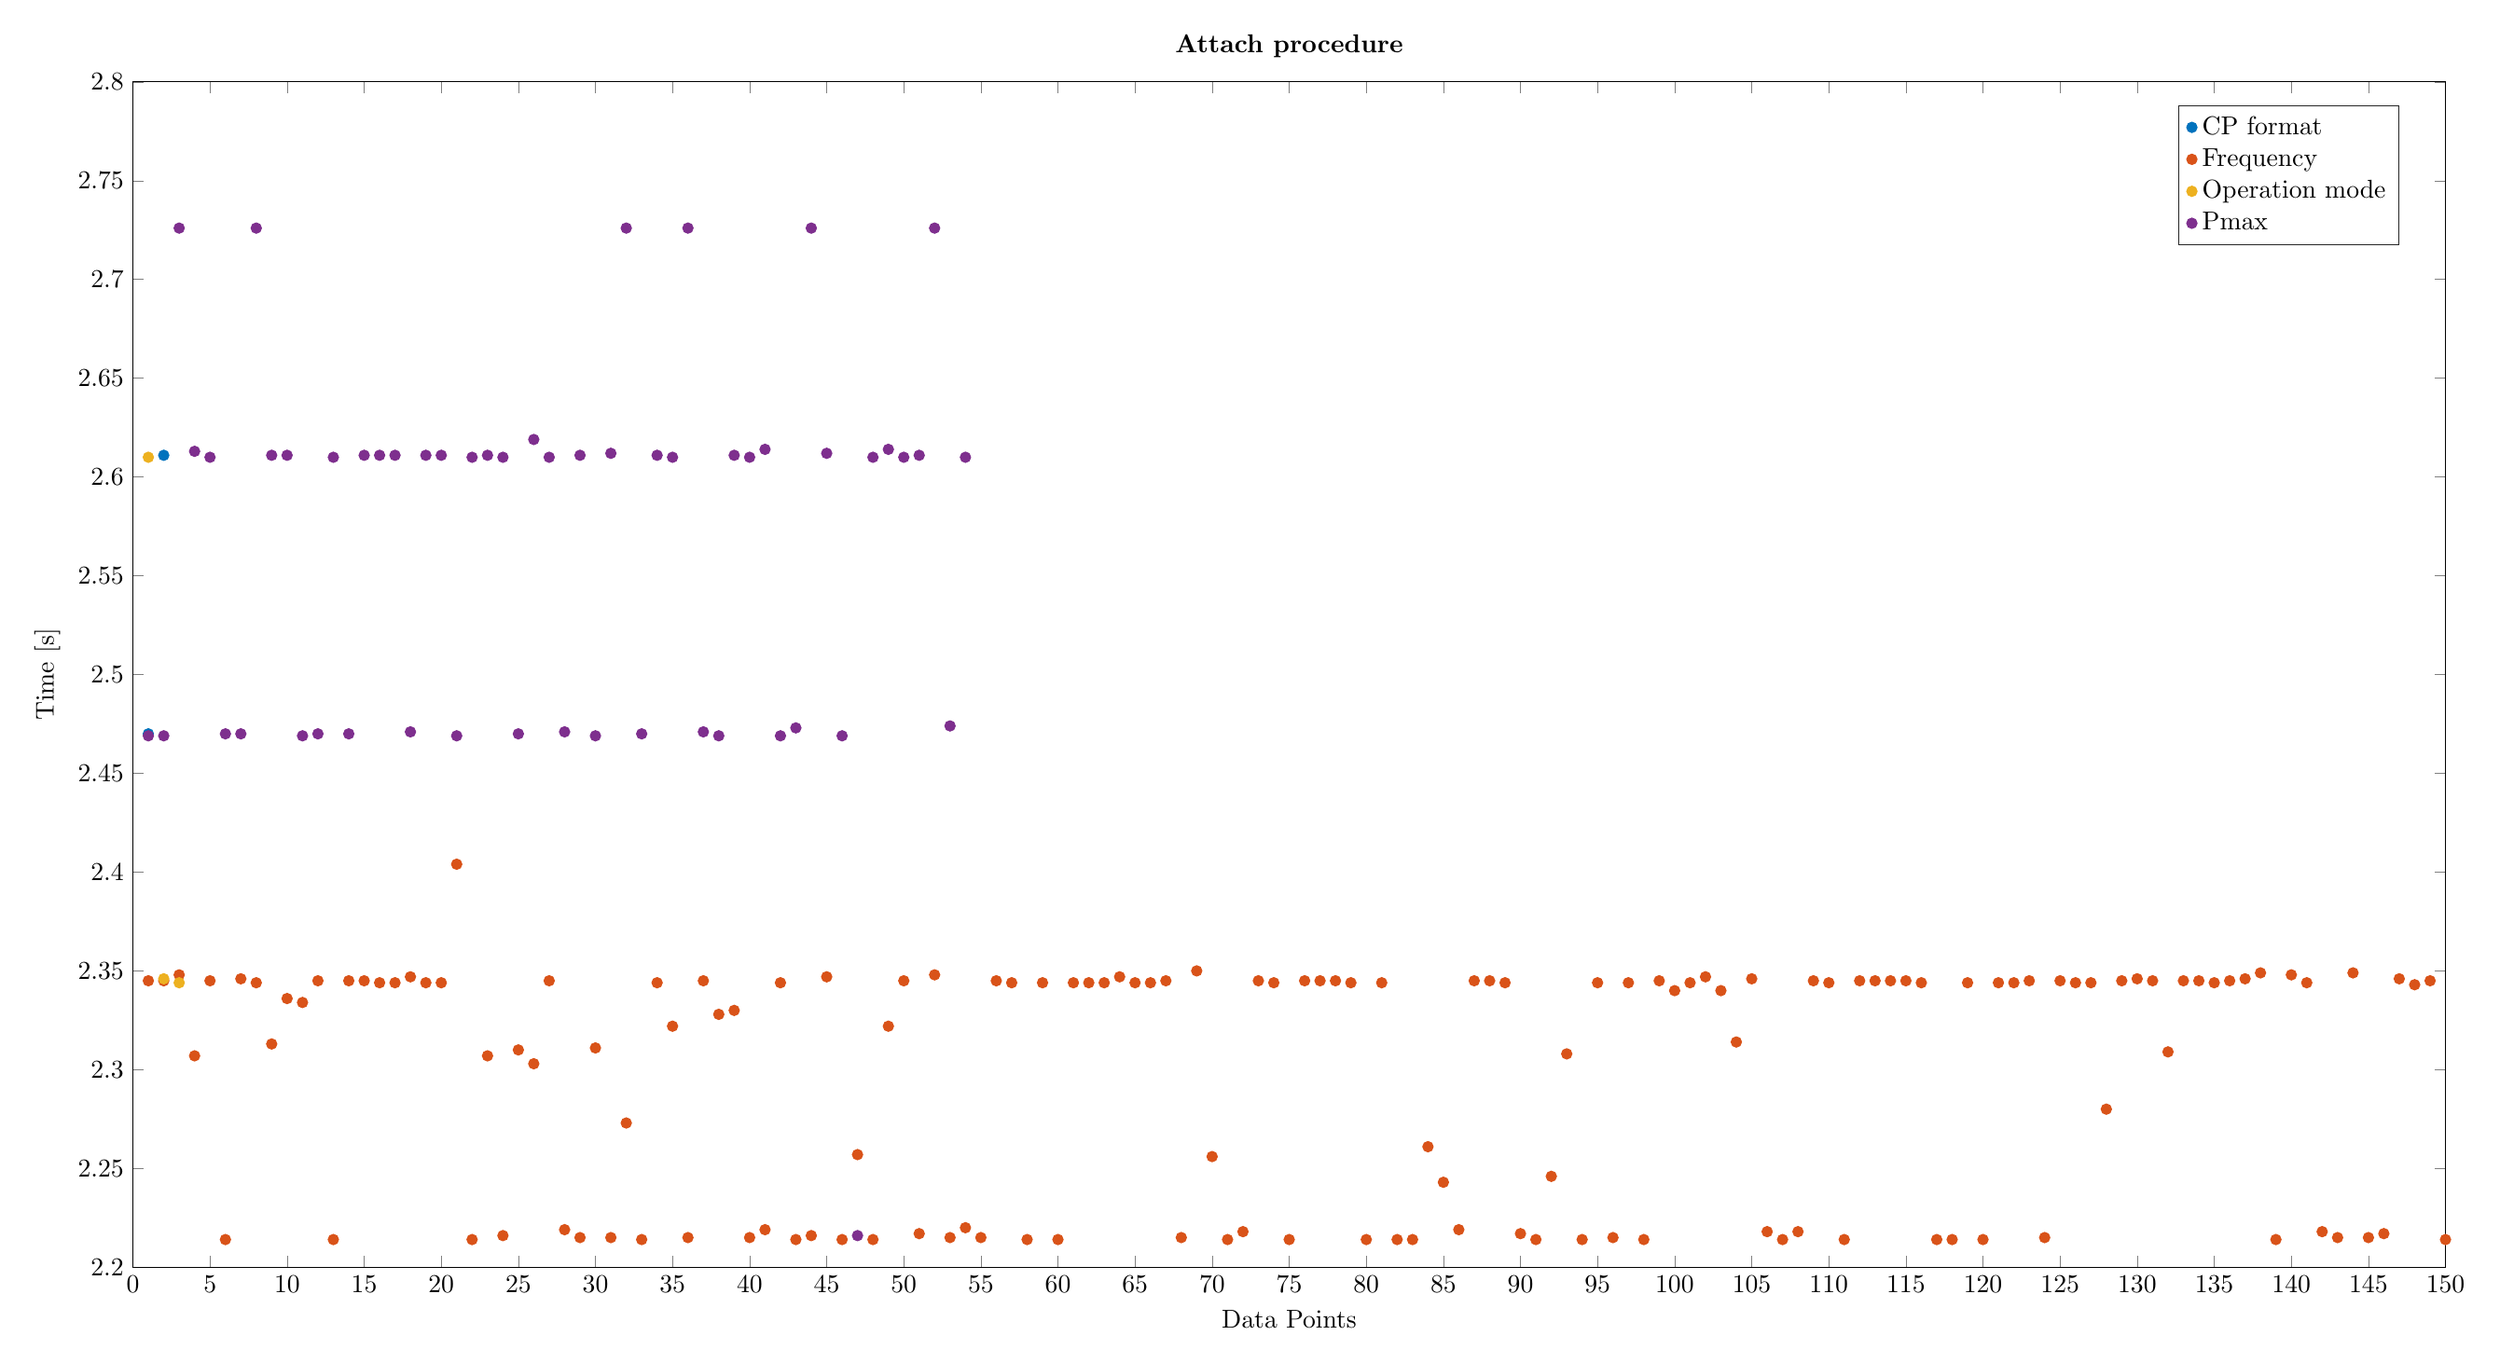
\begin{tikzpicture}

\begin{axis}[%
width=12.4in,
height=6.357in,
at={(2.08in,0.858in)},
scale only axis,
xmin=0,
xmax=150,
xlabel={Data Points},
ymin=2.2,
ymax=2.8,
ylabel={Time [s]},
axis background/.style={fill=white},
title style={font=\bfseries},
title={Attach procedure},
legend style={legend cell align=left,align=left,draw=white!15!black}
]
\addplot [color=mycolor1,only marks,mark=*,mark options={solid}]
  table[row sep=crcr]{%
1	2.47\\
2	2.611\\
};
\addlegendentry{CP format};

\addplot [color=mycolor2,only marks,mark=*,mark options={solid}]
  table[row sep=crcr]{%
1	2.345\\
2	2.345\\
3	2.348\\
4	2.307\\
5	2.345\\
6	2.214\\
7	2.346\\
8	2.344\\
9	2.313\\
10	2.336\\
11	2.334\\
12	2.345\\
13	2.214\\
14	2.345\\
15	2.345\\
16	2.344\\
17	2.344\\
18	2.347\\
19	2.344\\
20	2.344\\
21	2.404\\
22	2.214\\
23	2.307\\
24	2.216\\
25	2.31\\
26	2.30299999999999\\
27	2.345\\
28	2.219\\
29	2.215\\
30	2.31099999999999\\
31	2.215\\
32	2.273\\
33	2.214\\
34	2.344\\
35	2.32199999999999\\
36	2.215\\
37	2.345\\
38	2.328\\
39	2.33\\
40	2.215\\
41	2.219\\
42	2.344\\
43	2.214\\
44	2.216\\
45	2.347\\
46	2.214\\
47	2.25699999999999\\
48	2.214\\
49	2.32199999999999\\
50	2.345\\
51	2.217\\
52	2.348\\
53	2.215\\
54	2.22\\
55	2.215\\
56	2.345\\
57	2.344\\
58	2.214\\
59	2.344\\
60	2.214\\
61	2.344\\
62	2.344\\
63	2.344\\
64	2.347\\
65	2.344\\
66	2.344\\
67	2.345\\
68	2.215\\
69	2.35\\
70	2.256\\
71	2.214\\
72	2.218\\
73	2.345\\
74	2.344\\
75	2.214\\
76	2.345\\
77	2.345\\
78	2.345\\
79	2.344\\
80	2.214\\
81	2.344\\
82	2.214\\
83	2.214\\
84	2.261\\
85	2.243\\
86	2.219\\
87	2.345\\
88	2.345\\
89	2.344\\
90	2.217\\
91	2.214\\
92	2.246\\
93	2.308\\
94	2.214\\
95	2.344\\
96	2.215\\
97	2.344\\
98	2.214\\
99	2.345\\
100	2.34\\
101	2.344\\
102	2.347\\
103	2.34\\
104	2.31399999999999\\
105	2.346\\
106	2.218\\
107	2.214\\
108	2.218\\
109	2.345\\
110	2.344\\
111	2.214\\
112	2.345\\
113	2.345\\
114	2.345\\
115	2.345\\
116	2.344\\
117	2.214\\
118	2.214\\
119	2.344\\
120	2.214\\
121	2.344\\
122	2.344\\
123	2.345\\
124	2.215\\
125	2.345\\
126	2.344\\
127	2.344\\
128	2.28\\
129	2.345\\
130	2.346\\
131	2.345\\
132	2.309\\
133	2.345\\
134	2.345\\
135	2.344\\
136	2.345\\
137	2.346\\
138	2.349\\
139	2.214\\
140	2.348\\
141	2.344\\
142	2.218\\
143	2.215\\
144	2.349\\
145	2.215\\
146	2.217\\
147	2.346\\
148	2.343\\
149	2.345\\
150	2.214\\
};
\addlegendentry{Frequency};

\addplot [color=mycolor3,only marks,mark=*,mark options={solid}]
  table[row sep=crcr]{%
1	2.61\\
2	2.346\\
3	2.344\\
};
\addlegendentry{Operation mode};

\addplot [color=mycolor4,only marks,mark=*,mark options={solid}]
  table[row sep=crcr]{%
1	2.469\\
2	2.469\\
3	2.726\\
4	2.613\\
5	2.61\\
6	2.47\\
7	2.47\\
8	2.726\\
9	2.611\\
10	2.611\\
11	2.469\\
12	2.47\\
13	2.61\\
14	2.47\\
15	2.611\\
16	2.611\\
17	2.611\\
18	2.471\\
19	2.611\\
20	2.611\\
21	2.469\\
22	2.61\\
23	2.611\\
24	2.61\\
25	2.47\\
26	2.619\\
27	2.61\\
28	2.471\\
29	2.611\\
30	2.469\\
31	2.612\\
32	2.726\\
33	2.47\\
34	2.611\\
35	2.61\\
36	2.726\\
37	2.471\\
38	2.469\\
39	2.611\\
40	2.61\\
41	2.614\\
42	2.469\\
43	2.473\\
44	2.726\\
45	2.612\\
46	2.469\\
47	2.216\\
48	2.61\\
49	2.614\\
50	2.61\\
51	2.611\\
52	2.726\\
53	2.474\\
54	2.61\\
};
\addlegendentry{Pmax};

\end{axis}
\end{tikzpicture}%}
\end{minipage}
\hfill
\begin{minipage}{0.48\textwidth}
\tikzsetnextfilename{Attach_Time_Stat}
\resizebox{\textwidth}{!}{
% This file was created by matlab2tikz.
%
%The latest updates can be retrieved from
%  http://www.mathworks.com/matlabcentral/fileexchange/22022-matlab2tikz-matlab2tikz
%where you can also make suggestions and rate matlab2tikz.
%
%Point distribution 
%mean = 2.371081339712919 
%var = 0.019530805852043
%
\definecolor{mycolor1}{rgb}{0.00000,0.44700,0.74100}%
\definecolor{mycolor2}{rgb}{0.85000,0.32500,0.09800}%
%
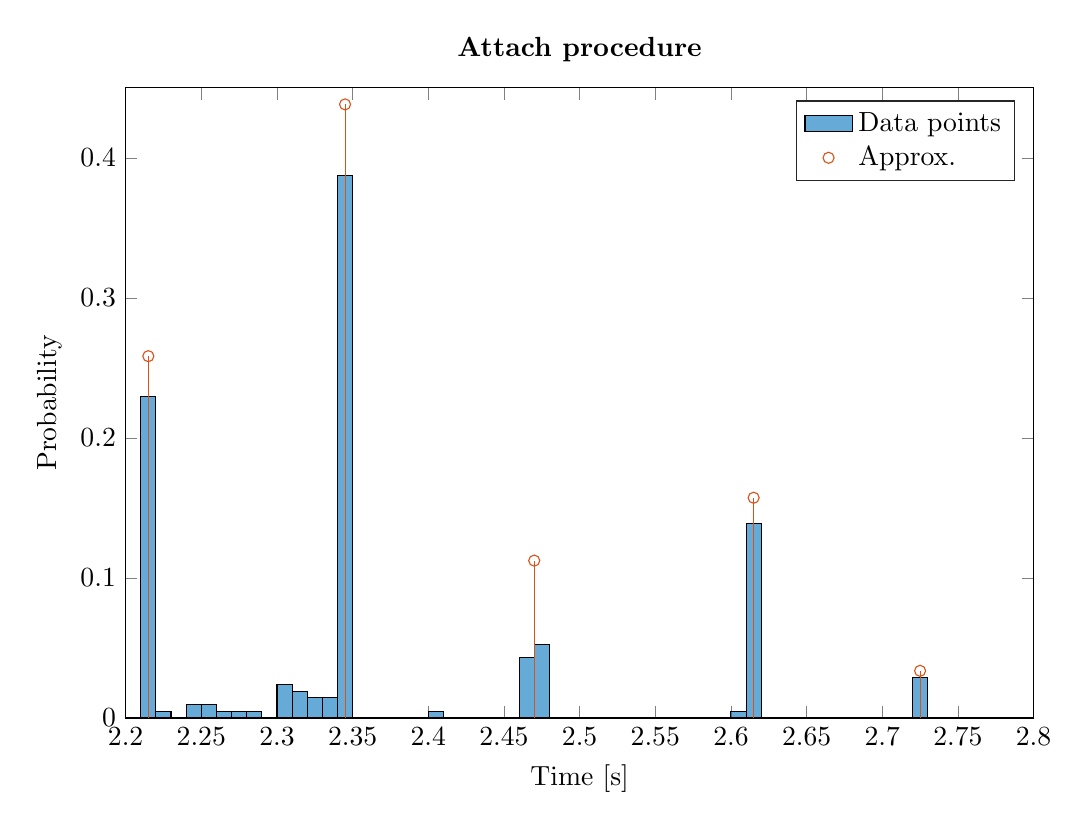
\begin{tikzpicture}

\begin{axis}[%
width=0.951\textwidth,
height=0.66\textwidth,
at={(0\textwidth,0\textwidth)},
scale only axis,
xmin=2.2,
xmax=2.8,
xlabel={Time [s]},
ymin=0,
ymax=0.45,
ylabel={Probability},
axis background/.style={fill=white},
title style={font=\bfseries},
title={Attach procedure},
legend style={legend cell align=left,align=left,draw=white!15!black},
y tick label style={/pgf/number format/fixed}
]
\addplot[fill=mycolor1,fill opacity=0.6,draw=black,ybar interval,area legend] plot table[row sep=crcr] {%
x	y\\
2.21	0.229665071770335\\
2.22	0.00478468899521531\\
2.23	0\\
2.24	0.00956937799043062\\
2.25	0.00956937799043062\\
2.26	0.00478468899521531\\
2.27	0.00478468899521531\\
2.28	0.00478468899521531\\
2.29	0\\
2.3	0.0239234449760766\\
2.31	0.0191387559808612\\
2.32	0.0143540669856459\\
2.33	0.0143540669856459\\
2.34	0.38755980861244\\
2.35	0\\
2.36	0\\
2.37	0\\
2.38	0\\
2.39	0\\
2.4	0.00478468899521531\\
2.41	0\\
2.42	0\\
2.43	0\\
2.44	0\\
2.45	0\\
2.46	0.0430622009569378\\
2.47	0.0526315789473684\\
2.48	0\\
2.49	0\\
2.5	0\\
2.51	0\\
2.52	0\\
2.53	0\\
2.54	0\\
2.55	0\\
2.56	0\\
2.57	0\\
2.58	0\\
2.59	0\\
2.6	0.00478468899521531\\
2.61	0.138755980861244\\
2.62	0\\
2.63	0\\
2.64	0\\
2.65	0\\
2.66	0\\
2.67	0\\
2.68	0\\
2.69	0\\
2.7	0\\
2.71	0\\
2.72	0.0287081339712919\\
2.73	0.0287081339712919\\
};
\addlegendentry{Data points};

\addplot[ycomb,color=mycolor2,solid,mark=o,mark options={solid}] plot table[row sep=crcr] 
\end{minipage}
\caption{Time spent during attach procedure.}
\label{fig:Attach_Time_Points}
\end{figure}

As can be seen in \autoref{fig:Attach_Time_Points} the time to attach seems to centered around certain values. This could very potentially be based on the occurrences of NPRACH occasions. Beside this none of the parameters seems to influence the time it takes. Because of this a point distribution is applied as it fits this scenario. 

The final element is the energy needed to release the the device. This is found based on area C which is the time after the attach is completed and until the power drops to just around zero. It is investigated like the attach element by splitting it up into power and time. The average power consumption is found based on \autoref{eq:power}. The result of which can be seen in \autoref{fig:Release_Power_Points}.

\begin{figure}[H]
\centering
\begin{minipage}{0.48\textwidth}
\tikzsetnextfilename{Release_Power_Points}
\resizebox{\textwidth}{!}{
% This file was created by matlab2tikz.
%
%The latest updates can be retrieved from
%  http://www.mathworks.com/matlabcentral/fileexchange/22022-matlab2tikz-matlab2tikz
%where you can also make suggestions and rate matlab2tikz.
%
\definecolor{mycolor1}{rgb}{0.00000,0.44700,0.74100}%
\definecolor{mycolor2}{rgb}{0.85000,0.32500,0.09800}%
\definecolor{mycolor3}{rgb}{0.92900,0.69400,0.12500}%
\definecolor{mycolor4}{rgb}{0.49400,0.18400,0.55600}%
%
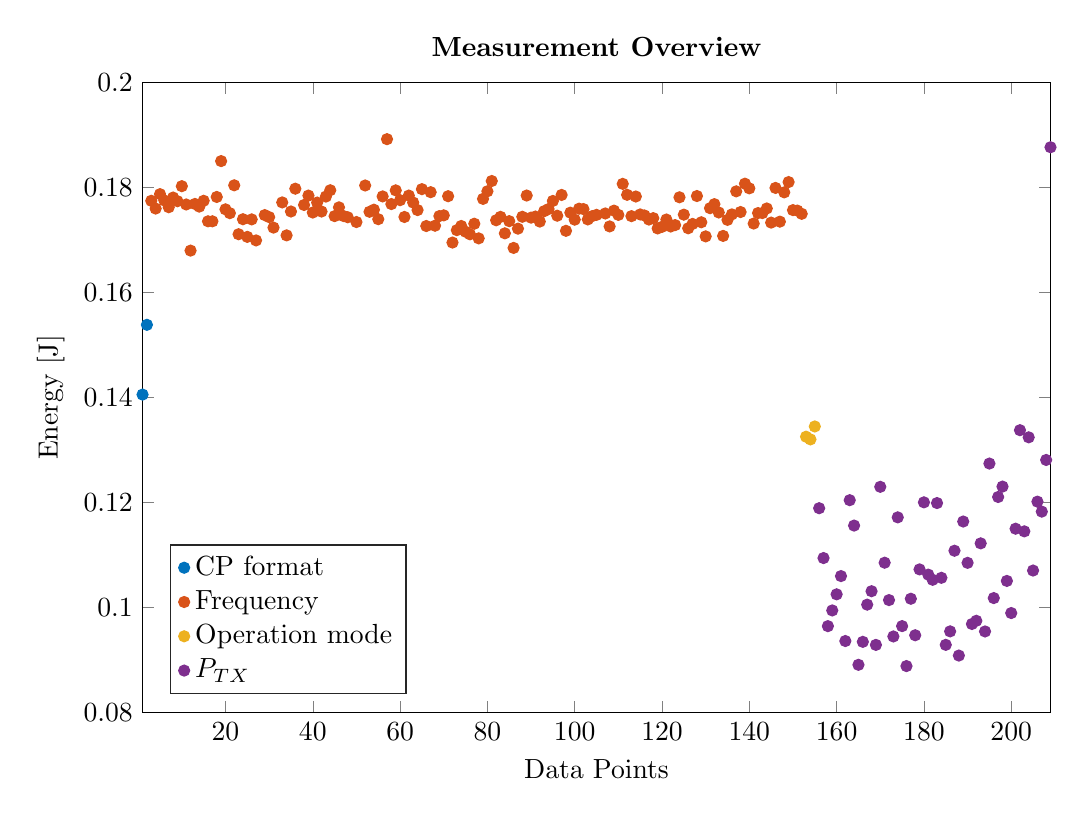
\begin{tikzpicture}

\begin{axis}[%
width=0.951\textwidth,
height=0.66\textwidth,
at={(0\textwidth,0\textwidth)},
scale only axis,
unbounded coords=jump,
xmin=1,
xmax=209,
xlabel={Data Points},
ymin=0.08,
ymax=0.2,
ylabel={Energy [J]},
axis background/.style={fill=white},
title style={font=\bfseries},
title={Measurement Overview},
legend style={at={(0.03,0.03)},anchor=south west,legend cell align=left,align=left,draw=white!15!black},
y tick label style={/pgf/number format/fixed}
]
\addplot [color=mycolor1,only marks,mark=*,mark options={solid}]
  table[row sep=crcr]{%
1	0.140568104547288\\
2	0.153853224763516\\
};
\addlegendentry{CP format};

\addplot [color=mycolor2,only marks,mark=*,mark options={solid}]
  table[row sep=crcr]{%
3	0.177470972694836\\
4	0.175992449744592\\
5	0.178738309089774\\
6	0.177528447958075\\
7	0.176247803427347\\
8	0.178088576766518\\
9	0.177392421916207\\
10	0.180254090835522\\
11	0.176769692397348\\
12	0.16798636401337\\
13	0.176872605685184\\
14	0.176363019491908\\
15	0.177472767635903\\
16	0.173566991672199\\
17	0.173562714836817\\
18	0.178200948080494\\
19	0.185031234017555\\
20	0.1758455036205\\
21	0.175116281149159\\
22	0.180421559134208\\
23	0.171105217020413\\
24	0.173963830459786\\
25	0.17060181324749\\
26	0.1739313670897\\
27	0.169926737829469\\
28	nan\\
29	0.174748321452\\
30	0.174366469192674\\
31	0.172365227327524\\
32	nan\\
33	0.177160825927427\\
34	0.170888181418621\\
35	0.175433522615405\\
36	0.179775458742444\\
37	nan\\
38	0.176675682890603\\
39	0.178460302723\\
40	0.175239169672574\\
41	0.177132530256322\\
42	0.175425505583809\\
43	0.178274096696072\\
44	0.179480539744956\\
45	0.174554290689458\\
46	0.176221364985752\\
47	0.174582632162135\\
48	0.174338269726251\\
49	nan\\
50	0.173423523764697\\
51	nan\\
52	0.180385819365891\\
53	0.175375675322284\\
54	0.175773232935549\\
55	0.173969521512958\\
56	0.178305606383167\\
57	0.189206203627575\\
58	0.176851797158872\\
59	0.179457137872274\\
60	0.177591510012864\\
61	0.174389927732811\\
62	0.178464886226564\\
63	0.177136641824962\\
64	0.175704631125638\\
65	0.179688623561719\\
66	0.172666214145131\\
67	0.179111764603052\\
68	0.172725900756085\\
69	0.174558493170143\\
70	0.174699965204281\\
71	0.178345502909064\\
72	0.169516929656635\\
73	0.171880428547195\\
74	0.172672477996908\\
75	0.171580034585017\\
76	0.171092418898708\\
77	0.173102987053828\\
78	0.170316269877042\\
79	0.177836573209014\\
80	0.179283643755348\\
81	0.181236961682121\\
82	0.173763026888087\\
83	0.174410265464304\\
84	0.171275744148354\\
85	0.173594759762126\\
86	0.168498135668041\\
87	0.172169071220076\\
88	0.174427017072488\\
89	0.178474682459102\\
90	0.174264190624066\\
91	0.174468744590075\\
92	0.173515711783502\\
93	0.175494781074804\\
94	0.175896979008889\\
95	0.177442656798844\\
96	0.174630976186465\\
97	0.178585296014539\\
98	0.171751561914703\\
99	0.175212939124332\\
100	0.173877032501164\\
101	0.175970180617463\\
102	0.175893765687646\\
103	0.173926420624751\\
104	0.174550037431466\\
105	0.174791542959422\\
106	nan\\
107	0.175058150329402\\
108	0.172591539813282\\
109	0.1755968056005\\
110	0.174788334775863\\
111	0.18069588407574\\
112	0.17861056700131\\
113	0.17454736470396\\
114	0.178288489308181\\
115	0.174873875698843\\
116	0.174670465017246\\
117	0.173899601184177\\
118	0.174169252279902\\
119	0.172209636983648\\
120	0.172511838432311\\
121	0.173904799269545\\
122	0.17257664190111\\
123	0.172844538997428\\
124	0.17813776992993\\
125	0.174831810533615\\
126	0.172240000156746\\
127	0.173066610547242\\
128	0.17837816122878\\
129	0.173381009665399\\
130	0.170694599032061\\
131	0.176066595812154\\
132	0.176831930467678\\
133	0.175246636556026\\
134	0.170784492293883\\
135	0.173838731675531\\
136	0.174882595028659\\
137	0.179271015733974\\
138	0.175331168376448\\
139	0.180728897115174\\
140	0.179840643613523\\
141	0.173139138453063\\
142	0.175136464136211\\
143	0.175135632157498\\
144	0.176008143774343\\
145	0.173317643644561\\
146	0.179921991178252\\
147	0.173502459879661\\
148	0.179080247349477\\
149	0.181036483452611\\
150	0.175697329741505\\
151	0.175604451768985\\
152	0.174990361966109\\
};
\addlegendentry{Frequency};

\addplot [color=mycolor3,only marks,mark=*,mark options={solid}]
  table[row sep=crcr]{%
153	0.132542496629046\\
154	0.132033590505031\\
155	0.134495673846313\\
};
\addlegendentry{Operation mode};

\addplot [color=mycolor4,only marks,mark=*,mark options={solid}]
  table[row sep=crcr]{%
156	0.118930546752406\\
157	0.109438867166733\\
158	0.0964726952969596\\
159	0.0994633008029128\\
160	0.102531314315504\\
161	0.106004577900469\\
162	0.0936375082952657\\
163	0.120458985916499\\
164	0.115623624714336\\
165	0.0891076563843949\\
166	0.0934812553057608\\
167	0.100565141229749\\
168	0.103124059025755\\
169	0.0929000476099331\\
170	0.123003023576874\\
171	0.108552397021186\\
172	0.101433978099906\\
173	0.0945069484596429\\
174	0.117187088354023\\
175	0.0964770664024355\\
176	0.0888662087289334\\
177	0.10168772598139\\
178	0.0947375934786839\\
179	0.107278319352022\\
180	0.12004605325136\\
181	0.106276782452598\\
182	0.105296910188876\\
183	0.119912954957721\\
184	0.105675685455486\\
185	0.0929095733354216\\
186	0.0954752780243934\\
187	0.110831492183349\\
188	0.0908713973489024\\
189	0.116395151919673\\
190	0.108526216098544\\
191	0.0968791917794761\\
192	0.0974876492361213\\
193	0.112237275772694\\
194	0.0954605570077646\\
195	0.127434664538977\\
196	0.101818015274907\\
197	0.121066202949429\\
198	0.123044887040781\\
199	0.105082535761505\\
200	0.0989646554007003\\
201	0.115024250511951\\
202	0.133788491362106\\
203	0.114522230873886\\
204	0.132429440887801\\
205	0.107061301401546\\
206	0.12017790186624\\
207	0.118281037642309\\
208	0.128117137471706\\
209	0.187668571046933\\
};
\addlegendentry{$P_{TX}$};

\end{axis}
\end{tikzpicture}%}
\end{minipage}
\hfill
\begin{minipage}{0.48\textwidth}
\tikzsetnextfilename{Release_Stat}
\resizebox{\textwidth}{!}{
% This file was created by matlab2tikz.
%
%The latest updates can be retrieved from
%  http://www.mathworks.com/matlabcentral/fileexchange/22022-matlab2tikz-matlab2tikz
%where you can also make suggestions and rate matlab2tikz.
%
%95% point = 0.179921991178252
%
\definecolor{mycolor1}{rgb}{0.00000,0.44700,0.74100}%
%
\begin{tikzpicture}

\begin{axis}[%
width=0.951\textwidth,
height=0.66\textwidth,
at={(0\textwidth,0\textwidth)},
scale only axis,
xmin=0.08,
xmax=0.2,
xlabel={Energy [J]},
ymin=0,
ymax=1,
ylabel={CDF},
axis background/.style={fill=white},
title style={font=\bfseries},
title={Statistical Overview},
y tick label style={/pgf/number format/fixed}
]
\addplot [color=mycolor1,solid,forget plot]
  table[row sep=crcr]{%
0.0888662087289334	0.00492610837438424\\
0.0891076563843949	0.00985221674876847\\
0.0908713973489024	0.0147783251231527\\
0.0929000476099331	0.0197044334975369\\
0.0929095733354216	0.0246305418719212\\
0.0934812553057608	0.0295566502463054\\
0.0936375082952657	0.0344827586206897\\
0.0945069484596429	0.0394088669950739\\
0.0947375934786839	0.0443349753694581\\
0.0954605570077646	0.0492610837438424\\
0.0954752780243934	0.0541871921182266\\
0.0964726952969596	0.0591133004926108\\
0.0964770664024355	0.0640394088669951\\
0.0968791917794761	0.0689655172413793\\
0.0974876492361213	0.0738916256157636\\
0.0989646554007003	0.0788177339901478\\
0.0994633008029128	0.083743842364532\\
0.100565141229749	0.0886699507389163\\
0.101433978099906	0.0935960591133005\\
0.10168772598139	0.0985221674876847\\
0.101818015274907	0.103448275862069\\
0.102531314315504	0.108374384236453\\
0.103124059025755	0.113300492610837\\
0.105082535761505	0.118226600985222\\
0.105296910188876	0.123152709359606\\
0.105675685455486	0.12807881773399\\
0.106004577900469	0.133004926108374\\
0.106276782452598	0.137931034482759\\
0.107061301401546	0.142857142857143\\
0.107278319352022	0.147783251231527\\
0.108526216098544	0.152709359605911\\
0.108552397021186	0.157635467980296\\
0.109438867166733	0.16256157635468\\
0.110831492183349	0.167487684729064\\
0.112237275772694	0.172413793103448\\
0.114522230873886	0.177339901477833\\
0.115024250511951	0.182266009852217\\
0.115623624714336	0.187192118226601\\
0.116395151919673	0.192118226600985\\
0.117187088354023	0.197044334975369\\
0.118281037642309	0.201970443349754\\
0.118930546752406	0.206896551724138\\
0.119912954957721	0.211822660098522\\
0.12004605325136	0.216748768472906\\
0.12017790186624	0.221674876847291\\
0.120458985916499	0.226600985221675\\
0.121066202949429	0.231527093596059\\
0.123003023576874	0.236453201970443\\
0.123044887040781	0.241379310344828\\
0.127434664538977	0.246305418719212\\
0.128117137471706	0.251231527093596\\
0.132033590505031	0.25615763546798\\
0.132429440887801	0.261083743842365\\
0.132542496629046	0.266009852216749\\
0.133788491362106	0.270935960591133\\
0.134495673846313	0.275862068965517\\
0.140568104547288	0.280788177339901\\
0.153853224763516	0.285714285714286\\
0.16798636401337	0.29064039408867\\
0.168498135668041	0.295566502463054\\
0.169516929656635	0.300492610837438\\
0.169926737829469	0.305418719211823\\
0.170316269877042	0.310344827586207\\
0.17060181324749	0.315270935960591\\
0.170694599032061	0.320197044334975\\
0.170784492293883	0.32512315270936\\
0.170888181418621	0.330049261083744\\
0.171092418898708	0.334975369458128\\
0.171105217020413	0.339901477832512\\
0.171275744148354	0.344827586206897\\
0.171580034585017	0.349753694581281\\
0.171751561914703	0.354679802955665\\
0.171880428547195	0.359605911330049\\
0.172169071220076	0.364532019704434\\
0.172209636983648	0.369458128078818\\
0.172240000156746	0.374384236453202\\
0.172365227327524	0.379310344827586\\
0.172511838432311	0.38423645320197\\
0.17257664190111	0.389162561576355\\
0.172591539813282	0.394088669950739\\
0.172666214145131	0.399014778325123\\
0.172672477996908	0.403940886699507\\
0.172725900756085	0.408866995073892\\
0.172844538997428	0.413793103448276\\
0.173066610547242	0.41871921182266\\
0.173102987053828	0.423645320197044\\
0.173139138453063	0.428571428571429\\
0.173317643644561	0.433497536945813\\
0.173381009665399	0.438423645320197\\
0.173423523764697	0.443349753694581\\
0.173502459879661	0.448275862068966\\
0.173515711783502	0.45320197044335\\
0.173562714836817	0.458128078817734\\
0.173566991672199	0.463054187192118\\
0.173594759762126	0.467980295566502\\
0.173763026888087	0.472906403940887\\
0.173838731675531	0.477832512315271\\
0.173877032501164	0.482758620689655\\
0.173899601184177	0.487684729064039\\
0.173904799269545	0.492610837438424\\
0.173926420624751	0.497536945812808\\
0.1739313670897	0.502463054187192\\
0.173963830459786	0.507389162561576\\
0.173969521512958	0.512315270935961\\
0.174169252279902	0.517241379310345\\
0.174264190624066	0.522167487684729\\
0.174338269726251	0.527093596059113\\
0.174366469192674	0.532019704433498\\
0.174389927732811	0.536945812807882\\
0.174410265464304	0.541871921182266\\
0.174427017072488	0.54679802955665\\
0.174468744590075	0.551724137931034\\
0.17454736470396	0.556650246305419\\
0.174550037431466	0.561576354679803\\
0.174554290689458	0.566502463054187\\
0.174558493170143	0.571428571428571\\
0.174582632162135	0.576354679802956\\
0.174630976186465	0.58128078817734\\
0.174670465017246	0.586206896551724\\
0.174699965204281	0.591133004926108\\
0.174748321452	0.596059113300493\\
0.174788334775863	0.600985221674877\\
0.174791542959422	0.605911330049261\\
0.174831810533615	0.610837438423645\\
0.174873875698843	0.61576354679803\\
0.174882595028659	0.620689655172414\\
0.174990361966109	0.625615763546798\\
0.175058150329402	0.630541871921182\\
0.175116281149159	0.635467980295567\\
0.175135632157498	0.640394088669951\\
0.175136464136211	0.645320197044335\\
0.175212939124332	0.650246305418719\\
0.175239169672574	0.655172413793103\\
0.175246636556026	0.660098522167488\\
0.175331168376448	0.665024630541872\\
0.175375675322284	0.669950738916256\\
0.175425505583809	0.67487684729064\\
0.175433522615405	0.679802955665025\\
0.175494781074804	0.684729064039409\\
0.1755968056005	0.689655172413793\\
0.175604451768985	0.694581280788177\\
0.175697329741505	0.699507389162562\\
0.175704631125638	0.704433497536946\\
0.175773232935549	0.70935960591133\\
0.1758455036205	0.714285714285714\\
0.175893765687646	0.719211822660099\\
0.175896979008889	0.724137931034483\\
0.175970180617463	0.729064039408867\\
0.175992449744592	0.733990147783251\\
0.176008143774343	0.738916256157635\\
0.176066595812154	0.74384236453202\\
0.176221364985752	0.748768472906404\\
0.176247803427347	0.753694581280788\\
0.176363019491908	0.758620689655172\\
0.176675682890603	0.763546798029557\\
0.176769692397348	0.768472906403941\\
0.176831930467678	0.773399014778325\\
0.176851797158872	0.778325123152709\\
0.176872605685184	0.783251231527094\\
0.177132530256322	0.788177339901478\\
0.177136641824962	0.793103448275862\\
0.177160825927427	0.798029556650246\\
0.177392421916207	0.802955665024631\\
0.177442656798844	0.807881773399015\\
0.177470972694836	0.812807881773399\\
0.177472767635903	0.817733990147783\\
0.177528447958075	0.822660098522167\\
0.177591510012864	0.827586206896552\\
0.177836573209014	0.832512315270936\\
0.178088576766518	0.83743842364532\\
0.17813776992993	0.842364532019704\\
0.178200948080494	0.847290640394089\\
0.178274096696072	0.852216748768473\\
0.178288489308181	0.857142857142857\\
0.178305606383167	0.862068965517241\\
0.178345502909064	0.866995073891626\\
0.17837816122878	0.87192118226601\\
0.178460302723	0.876847290640394\\
0.178464886226564	0.881773399014778\\
0.178474682459102	0.886699507389163\\
0.178585296014539	0.891625615763547\\
0.17861056700131	0.896551724137931\\
0.178738309089774	0.901477832512315\\
0.179080247349477	0.9064039408867\\
0.179111764603052	0.911330049261084\\
0.179271015733974	0.916256157635468\\
0.179283643755348	0.921182266009852\\
0.179457137872274	0.926108374384236\\
0.179480539744956	0.931034482758621\\
0.179688623561719	0.935960591133005\\
0.179775458742444	0.940886699507389\\
0.179840643613523	0.945812807881773\\
0.179921991178252	0.950738916256158\\
0.180254090835522	0.955665024630542\\
0.180385819365891	0.960591133004926\\
0.180421559134208	0.96551724137931\\
0.18069588407574	0.970443349753695\\
0.180728897115174	0.975369458128079\\
0.181036483452611	0.980295566502463\\
0.181236961682121	0.985221674876847\\
0.185031234017555	0.990147783251232\\
0.187668571046933	0.995073891625616\\
0.189206203627575	1\\
};
\end{axis}
\end{tikzpicture}%}
\end{minipage}
\caption{Average power consumption during release sequence.}
\label{fig:Release_Power_Points}
\end{figure}

%In the same sense as with the power two peaks can be seen here, but again a unimodal distribution is used as no explanation is known to do otherwise. A little surprisingly it does not seem that the $P_{TX}$ has any significant influence on the energy consumption. It is chosen to use a lognormal distribution for the same reasoning as with the average power consumption for the attach procedure.   
It is seen from \autoref{fig:Release_Power_Points}, that the $P_{TX}$ has an influence, however compared to the influence on the attach procedure the impact is not nearly as defined. It is believe to be because to the energy is mainly spent on RX instead of TX. Likewise the other parameters their own mean value which should not be the case since they share points across the measurements. What can be taken from this is the model does not really support a complicated scenario like a release procedure. Because of this a statistical analysis of the distribution does not make much sense, however instead the value for which 95\% of the measurements is contained is found based on a CDF of the data. 

The time to do the release sequence is found based on \autoref{eq:time} for area C. This is done for all the measurements and the result can be seen in \autoref{fig:Release_Time_Points}. 

\begin{figure}[H]
\centering
\begin{minipage}{0.48\textwidth}
\tikzsetnextfilename{Release_Time_Points}
\resizebox{\textwidth}{!}{
% This file was created by matlab2tikz.
%
%The latest updates can be retrieved from
%  http://www.mathworks.com/matlabcentral/fileexchange/22022-matlab2tikz-matlab2tikz
%where you can also make suggestions and rate matlab2tikz.
%
\definecolor{mycolor1}{rgb}{0.00000,0.44700,0.74100}%
\definecolor{mycolor2}{rgb}{0.85000,0.32500,0.09800}%
\definecolor{mycolor3}{rgb}{0.92900,0.69400,0.12500}%
\definecolor{mycolor4}{rgb}{0.49400,0.18400,0.55600}%
%
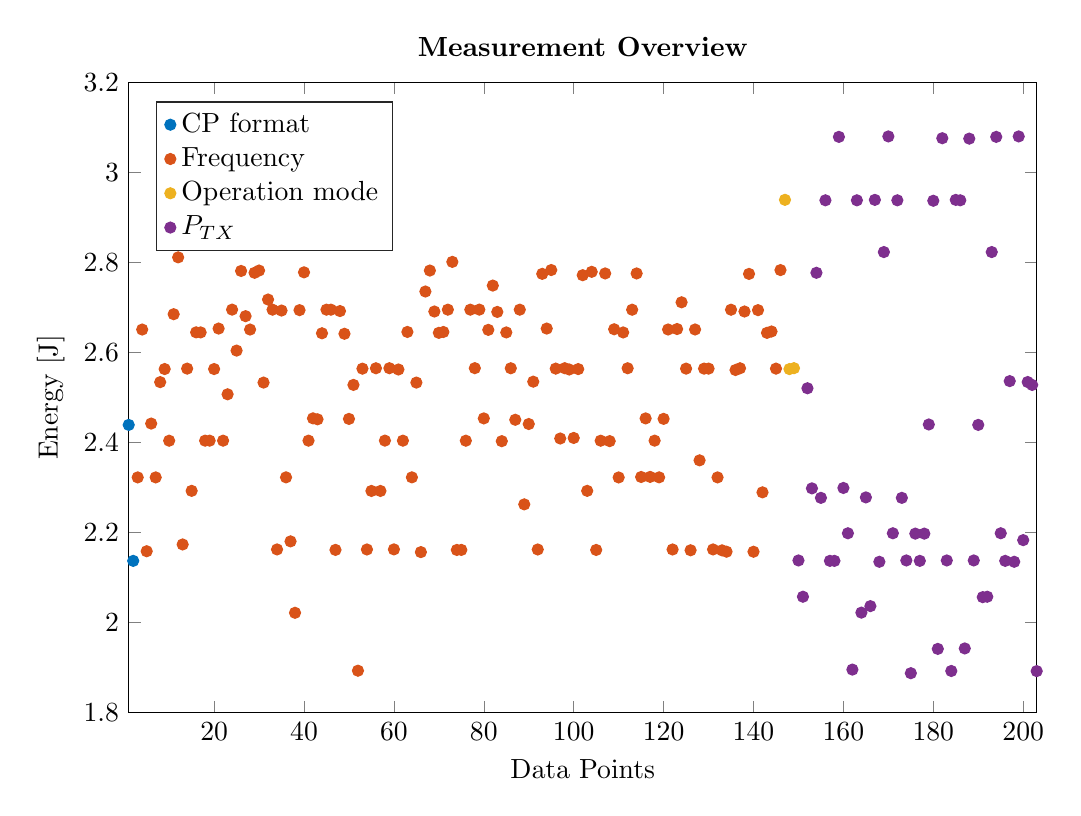
\begin{tikzpicture}

\begin{axis}[%
width=0.951\textwidth,
height=0.66\textwidth,
at={(0\textwidth,0\textwidth)},
scale only axis,
xmin=1,
xmax=203,
xlabel={Data Points},
ymin=1.8,
ymax=3.2,
ylabel={Energy [J]},
axis background/.style={fill=white},
title style={font=\bfseries},
title={Measurement Overview},
legend style={at={(0.03,0.97)},anchor=north west,legend cell align=left,align=left,draw=white!15!black},
y tick label style={/pgf/number format/fixed}
]
\addplot [color=mycolor1,only marks,mark=*,mark options={solid}]
  table[row sep=crcr]{%
1	2.4392704\\
2	2.1371904\\
};
\addlegendentry{CP format};

\addplot [color=mycolor2,only marks,mark=*,mark options={solid}]
  table[row sep=crcr]{%
3	2.3226368\\
4	2.651136\\
5	2.158592\\
6	2.44224\\
7	2.3226368\\
8	2.5342976\\
9	2.5633792\\
10	2.4041472\\
11	2.6852352\\
12	2.8114944\\
13	2.1736448\\
14	2.5643008\\
15	2.292736\\
16	2.6448896\\
17	2.6447872\\
18	2.4042496\\
19	2.4042496\\
20	2.5633792\\
21	2.6532864\\
22	2.4042496\\
23	2.507264\\
24	2.6953728\\
25	2.6043392\\
26	2.7812864\\
27	2.680832\\
28	2.651136\\
29	2.7771904\\
30	2.782208\\
31	2.5332736\\
32	2.7177984\\
33	2.6952704\\
34	2.1625856\\
35	2.6933248\\
36	2.3227392\\
37	2.1805056\\
38	2.0217856\\
39	2.6942464\\
40	2.7782144\\
41	2.4042496\\
42	2.4538112\\
43	2.4516608\\
44	2.6428416\\
45	2.6952704\\
46	2.6952704\\
47	2.1615616\\
48	2.6921984\\
49	2.6417152\\
50	2.4525824\\
51	2.5281536\\
52	1.8931712\\
53	2.5641984\\
54	2.1624832\\
55	2.2925312\\
56	2.56512\\
57	2.2925312\\
58	2.404352\\
59	2.5652224\\
60	2.162688\\
61	2.5623552\\
62	2.4042496\\
63	2.6458112\\
64	2.3227392\\
65	2.5332736\\
66	2.1566464\\
67	2.735616\\
68	2.782208\\
69	2.6911744\\
70	2.6437632\\
71	2.6457088\\
72	2.6952704\\
73	2.8014592\\
74	2.1614592\\
75	2.1615616\\
76	2.4041472\\
77	2.6952704\\
78	2.5653248\\
79	2.6953728\\
80	2.4537088\\
81	2.6504192\\
82	2.7488256\\
83	2.6902528\\
84	2.4031232\\
85	2.6446848\\
86	2.56512\\
87	2.4506368\\
88	2.6952704\\
89	2.2627328\\
90	2.441216\\
91	2.5353216\\
92	2.1624832\\
93	2.77483519999999\\
94	2.6532864\\
95	2.7833344\\
96	2.5643008\\
97	2.4090624\\
98	2.5652224\\
99	2.5623552\\
100	2.4102912\\
101	2.5632768\\
102	2.7718656\\
103	2.292736\\
104	2.7793408\\
105	2.1614592\\
106	2.4041472\\
107	2.7757568\\
108	2.4032256\\
109	2.6517504\\
110	2.3225344\\
111	2.6446848\\
112	2.56512\\
113	2.695168\\
114	2.7757568\\
115	2.3235584\\
116	2.4537088\\
117	2.3237632\\
118	2.4042496\\
119	2.3227392\\
120	2.4526848\\
121	2.6512384\\
122	2.1624832\\
123	2.6522624\\
124	2.7116544\\
125	2.5643008\\
126	2.1607424\\
127	2.6512384\\
128	2.3605248\\
129	2.5643008\\
130	2.5643008\\
131	2.1625856\\
132	2.3226368\\
133	2.1605376\\
134	2.157568\\
135	2.695168\\
136	2.5612288\\
137	2.56512\\
138	2.6911744\\
139	2.7747328\\
140	2.1574656\\
141	2.6942464\\
142	2.2894592\\
143	2.6437632\\
144	2.6468352\\
145	2.5643008\\
146	2.783232\\
};
\addlegendentry{Frequency};

\addplot [color=mycolor3,only marks,mark=*,mark options={solid}]
  table[row sep=crcr]{%
147	2.9392896\\
148	2.5632768\\
149	2.5653248\\
};
\addlegendentry{Operation mode};

\addplot [color=mycolor4,only marks,mark=*,mark options={solid}]
  table[row sep=crcr]{%
150	2.138112\\
151	2.0575232\\
152	2.5206784\\
153	2.2982656\\
154	2.77719040000001\\
155	2.2771712\\
156	2.9382656\\
157	2.1371904\\
158	2.1371904\\
159	3.079168\\
160	2.2991872\\
161	2.198528\\
162	1.8956288\\
163	2.9382656\\
164	2.0221952\\
165	2.2781952\\
166	2.0366336\\
167	2.9391872\\
168	2.1351424\\
169	2.8232704\\
170	3.080192\\
171	2.198528\\
172	2.9382656\\
173	2.2771712\\
174	2.138112\\
175	1.8876416\\
176	2.1977088\\
177	2.1371904\\
178	2.1977088\\
179	2.440192\\
180	2.9372416\\
181	1.9416064\\
182	3.0761984\\
183	2.138112\\
184	1.8925568\\
185	2.9391872\\
186	2.9382656\\
187	1.9426304\\
188	3.0752768\\
189	2.138112\\
190	2.4392704\\
191	2.0566016\\
192	2.0575232\\
193	2.8232704\\
194	3.079168\\
195	2.198528\\
196	2.1371904\\
197	2.5365504\\
198	2.1351424\\
199	3.080192\\
200	2.1832704\\
201	2.5345024\\
202	2.5280512\\
203	1.8922496\\
};
\addlegendentry{$P_{TX}$};

\end{axis}
\end{tikzpicture}%}
\end{minipage}
\hfill
\begin{minipage}{0.48\textwidth}
\tikzsetnextfilename{Release_Time_Stat1}
\resizebox{\textwidth}{!}{
% This file was created by matlab2tikz.
%
%The latest updates can be retrieved from
%  http://www.mathworks.com/matlabcentral/fileexchange/22022-matlab2tikz-matlab2tikz
%where you can also make suggestions and rate matlab2tikz.
%
%Lognormal distribution 
%mean = 2.412161837320576 
%var = 0.245798445383439
%
\definecolor{mycolor1}{rgb}{0.00000,0.44700,0.74100}%
%
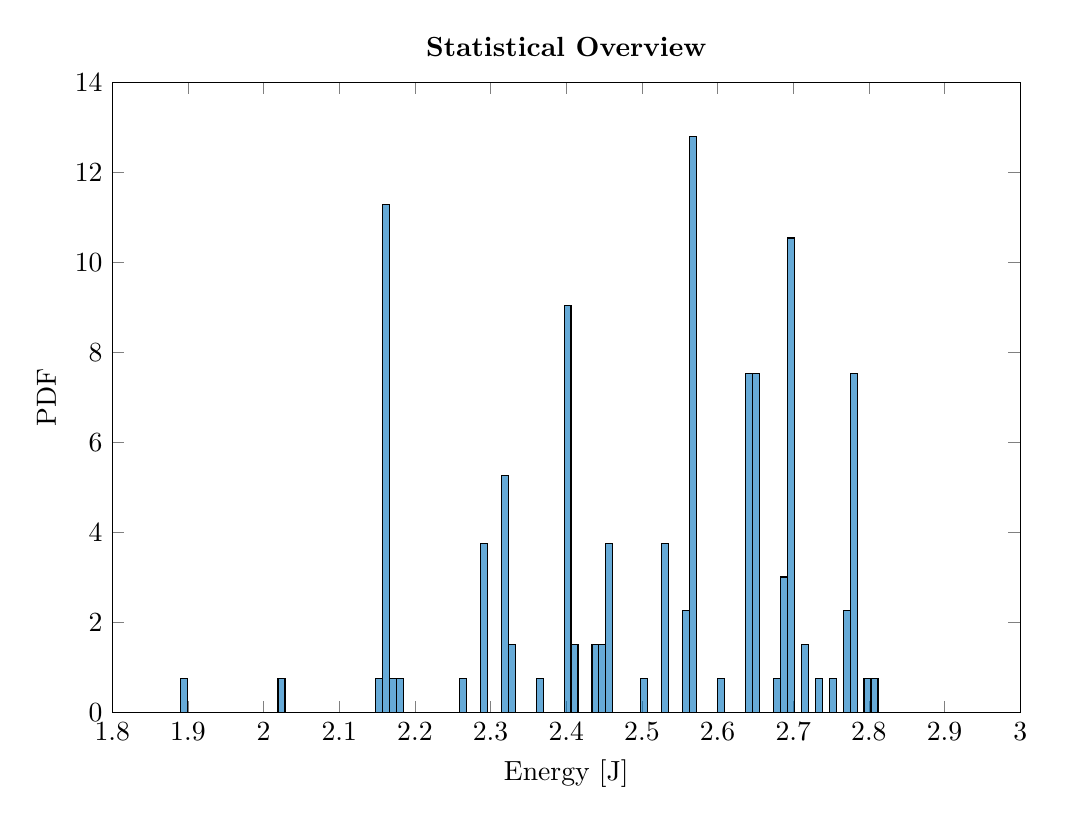
\begin{tikzpicture}

\begin{axis}[%
width=0.951\textwidth,
height=0.66\textwidth,
at={(0\textwidth,0\textwidth)},
scale only axis,
xmin=1.8,
xmax=3,
xlabel={Energy [J]},
ymin=0,
ymax=14,
ylabel={PDF},
axis background/.style={fill=white},
title style={font=\bfseries},
title={Statistical Overview},
y tick label style={/pgf/number format/fixed}
]
\addplot[fill=mycolor1,fill opacity=0.6,draw=black,ybar interval,area legend] plot table[row sep=crcr] {%
x	y\\
1.89	0.753193540612195\\
1.89922	0\\
1.90844	0\\
1.91766	0\\
1.92688	0\\
1.9361	0\\
1.94532	0\\
1.95454	0\\
1.96376	0\\
1.97298	0\\
1.9822	0\\
1.99142	0\\
2.00064	0\\
2.00986	0\\
2.01908	0.753193540612195\\
2.0283	0\\
2.03752	0\\
2.04674	0\\
2.05596	0\\
2.06518	0\\
2.0744	0\\
2.08362	0\\
2.09284	0\\
2.10206	0\\
2.11128	0\\
2.1205	0\\
2.12972	0\\
2.13894	0\\
2.14816	0.753193540612195\\
2.15738	11.2979031091829\\
2.1666	0.753193540612195\\
2.17582	0.753193540612195\\
2.18504	0\\
2.19426	0\\
2.20348	0\\
2.2127	0\\
2.22192	0\\
2.23114	0\\
2.24036	0\\
2.24958	0\\
2.2588	0.753193540612195\\
2.26802	0\\
2.27724	0\\
2.28646	3.76596770306098\\
2.29568	0\\
2.3049	0\\
2.31412	5.27235478428537\\
2.32334	1.50638708122439\\
2.33256	0\\
2.34178	0\\
2.351	0\\
2.36022	0.753193540612195\\
2.36944	0\\
2.37866	0\\
2.38788	0\\
2.3971	9.03832248734634\\
2.40632	1.50638708122439\\
2.41554	0\\
2.42476	0\\
2.43398	1.50638708122439\\
2.4432	1.50638708122439\\
2.45242	3.76596770306098\\
2.46164	0\\
2.47086	0\\
2.48008	0\\
2.4893	0\\
2.49852	0.753193540612195\\
2.50774	0\\
2.51696	0\\
2.52618	3.76596770306098\\
2.5354	0\\
2.54462	0\\
2.55384	2.25958062183659\\
2.56306	12.8042901904073\\
2.57228	0\\
2.5815	0\\
2.59072	0\\
2.59994	0.753193540612195\\
2.60916	0\\
2.61838	0\\
2.6276	0\\
2.63682	7.53193540612195\\
2.64604	7.53193540612195\\
2.65526	0\\
2.66448	0\\
2.6737	0.753193540612195\\
2.68292	3.01277416244878\\
2.69214	10.5447095685707\\
2.70136	0\\
2.71058	1.50638708122439\\
2.7198	0\\
2.72902	0.753193540612195\\
2.73824	0\\
2.74746	0.753193540612195\\
2.75668	0\\
2.7659	2.25958062183659\\
2.77512	7.53193540612195\\
2.78434	0\\
2.79356	0.753193540612195\\
2.80278	0.753193540612195\\
2.812	0.753193540612195\\
};
\end{axis}
\end{tikzpicture}%}
\end{minipage}
\caption{Time spent during release sequence.}
\label{fig:Release_Time_Points}
\end{figure}

It can be seen that the time it takes to release the device from the network varies a lot. Based on the networks structure, restrictions are made about how long time it can take, but to account for all the values with e.g. a point distribution is not really feasible. Because of this the same trick is applied as with the average power consumption and the 95\% point is found based on the CDF of the data, which can be seen in \autoref{fig:Release_Time_Stat2}.

\begin{figure}[H]
\centering
\begin{minipage}{0.48\textwidth}
\tikzsetnextfilename{Release_Time_Stat2}
\resizebox{\textwidth}{!}{
% This file was created by matlab2tikz.
%
%The latest updates can be retrieved from
%  http://www.mathworks.com/matlabcentral/fileexchange/22022-matlab2tikz-matlab2tikz
%where you can also make suggestions and rate matlab2tikz.
%
%95% point = 2.938265600000001
%
\definecolor{mycolor1}{rgb}{0.00000,0.44700,0.74100}%
%
\begin{tikzpicture}

\begin{axis}[%
width=0.951\textwidth,
height=0.66\textwidth,
at={(0\textwidth,0\textwidth)},
scale only axis,
xmin=1.8,
xmax=3.2,
xlabel={Energy [J]},
ymin=0,
ymax=1,
ylabel={CDF},
axis background/.style={fill=white},
title style={font=\bfseries},
title={Statistical Overview},
y tick label style={/pgf/number format/fixed}
]
\addplot [color=mycolor1,solid,forget plot]
  table[row sep=crcr]{%
1.8876416	0.00492610837438424\\
1.8922496	0.00985221674876847\\
1.8925568	0.0147783251231527\\
1.8931712	0.0197044334975369\\
1.8956288	0.0246305418719212\\
1.9416064	0.0295566502463054\\
1.9426304	0.0344827586206897\\
2.0217856	0.0394088669950739\\
2.0221952	0.0443349753694581\\
2.0366336	0.0492610837438424\\
2.0566016	0.0541871921182266\\
2.0575232	0.0591133004926108\\
2.0575232	0.0640394088669951\\
2.1351424	0.0689655172413793\\
2.1351424	0.0738916256157636\\
2.1371904	0.0788177339901478\\
2.1371904	0.083743842364532\\
2.1371904	0.0886699507389163\\
2.1371904	0.0935960591133005\\
2.1371904	0.0985221674876847\\
2.138112	0.103448275862069\\
2.138112	0.108374384236453\\
2.138112	0.113300492610837\\
2.138112	0.118226600985222\\
2.1566464	0.123152709359606\\
2.1574656	0.12807881773399\\
2.157568	0.133004926108374\\
2.158592	0.137931034482759\\
2.1605376	0.142857142857143\\
2.1607424	0.147783251231527\\
2.1614592	0.152709359605911\\
2.1614592	0.157635467980296\\
2.1615616	0.16256157635468\\
2.1615616	0.167487684729064\\
2.1624832	0.172413793103448\\
2.1624832	0.177339901477833\\
2.1624832	0.182266009852217\\
2.1625856	0.187192118226601\\
2.1625856	0.192118226600985\\
2.162688	0.197044334975369\\
2.1736448	0.201970443349754\\
2.1805056	0.206896551724138\\
2.1832704	0.211822660098522\\
2.1977088	0.216748768472906\\
2.1977088	0.221674876847291\\
2.198528	0.226600985221675\\
2.198528	0.231527093596059\\
2.198528	0.236453201970443\\
2.2627328	0.241379310344828\\
2.2771712	0.246305418719212\\
2.2771712	0.251231527093596\\
2.2781952	0.25615763546798\\
2.2894592	0.261083743842365\\
2.2925312	0.266009852216749\\
2.2925312	0.270935960591133\\
2.292736	0.275862068965517\\
2.292736	0.280788177339901\\
2.2982656	0.285714285714286\\
2.2991872	0.29064039408867\\
2.3225344	0.295566502463054\\
2.3226368	0.300492610837438\\
2.3226368	0.305418719211823\\
2.3226368	0.310344827586207\\
2.3227392	0.315270935960591\\
2.3227392	0.320197044334975\\
2.3227392	0.32512315270936\\
2.3235584	0.330049261083744\\
2.3237632	0.334975369458128\\
2.3605248	0.339901477832512\\
2.4031232	0.344827586206897\\
2.4032256	0.349753694581281\\
2.4041472	0.354679802955665\\
2.4041472	0.359605911330049\\
2.4041472	0.364532019704434\\
2.4042496	0.369458128078818\\
2.4042496	0.374384236453202\\
2.4042496	0.379310344827586\\
2.4042496	0.38423645320197\\
2.4042496	0.389162561576355\\
2.4042496	0.394088669950739\\
2.404352	0.399014778325123\\
2.4090624	0.403940886699507\\
2.4102912	0.408866995073892\\
2.4392704	0.413793103448276\\
2.4392704	0.41871921182266\\
2.440192	0.423645320197044\\
2.441216	0.428571428571429\\
2.44224	0.433497536945813\\
2.4506368	0.438423645320197\\
2.4516608	0.443349753694581\\
2.4525824	0.448275862068966\\
2.4526848	0.45320197044335\\
2.4537088	0.458128078817734\\
2.4537088	0.463054187192118\\
2.4538112	0.467980295566502\\
2.507264	0.472906403940887\\
2.5206784	0.477832512315271\\
2.5280512	0.482758620689655\\
2.5281536	0.487684729064039\\
2.5332736	0.492610837438424\\
2.5332736	0.497536945812808\\
2.5342976	0.502463054187192\\
2.5345024	0.507389162561576\\
2.5353216	0.512315270935961\\
2.5365504	0.517241379310345\\
2.5612288	0.522167487684729\\
2.5623552	0.527093596059113\\
2.5623552	0.532019704433498\\
2.5632768	0.536945812807882\\
2.5632768	0.541871921182266\\
2.5633792	0.54679802955665\\
2.5633792	0.551724137931034\\
2.5641984	0.556650246305419\\
2.5643008	0.561576354679803\\
2.5643008	0.566502463054187\\
2.5643008	0.571428571428571\\
2.5643008	0.576354679802956\\
2.5643008	0.58128078817734\\
2.5643008	0.586206896551724\\
2.56512	0.591133004926108\\
2.56512	0.596059113300493\\
2.56512	0.600985221674877\\
2.56512	0.605911330049261\\
2.5652224	0.610837438423645\\
2.5652224	0.61576354679803\\
2.5653248	0.620689655172414\\
2.5653248	0.625615763546798\\
2.6043392	0.630541871921182\\
2.6417152	0.635467980295567\\
2.6428416	0.640394088669951\\
2.6437632	0.645320197044335\\
2.6437632	0.650246305418719\\
2.6446848	0.655172413793103\\
2.6446848	0.660098522167488\\
2.6447872	0.665024630541872\\
2.6448896	0.669950738916256\\
2.6457088	0.67487684729064\\
2.6458112	0.679802955665025\\
2.6468352	0.684729064039409\\
2.6504192	0.689655172413793\\
2.651136	0.694581280788177\\
2.651136	0.699507389162562\\
2.6512384	0.704433497536946\\
2.6512384	0.70935960591133\\
2.6517504	0.714285714285714\\
2.6522624	0.719211822660099\\
2.6532864	0.724137931034483\\
2.6532864	0.729064039408867\\
2.680832	0.733990147783251\\
2.6852352	0.738916256157635\\
2.6902528	0.74384236453202\\
2.6911744	0.748768472906404\\
2.6911744	0.753694581280788\\
2.6921984	0.758620689655172\\
2.6933248	0.763546798029557\\
2.6942464	0.768472906403941\\
2.6942464	0.773399014778325\\
2.695168	0.778325123152709\\
2.695168	0.783251231527094\\
2.6952704	0.788177339901478\\
2.6952704	0.793103448275862\\
2.6952704	0.798029556650246\\
2.6952704	0.802955665024631\\
2.6952704	0.807881773399015\\
2.6952704	0.812807881773399\\
2.6953728	0.817733990147783\\
2.6953728	0.822660098522167\\
2.7116544	0.827586206896552\\
2.7177984	0.832512315270936\\
2.735616	0.83743842364532\\
2.7488256	0.842364532019704\\
2.7718656	0.847290640394089\\
2.7747328	0.852216748768473\\
2.77483519999999	0.857142857142857\\
2.7757568	0.862068965517241\\
2.7757568	0.866995073891626\\
2.7771904	0.87192118226601\\
2.77719040000001	0.876847290640394\\
2.7782144	0.881773399014778\\
2.7793408	0.886699507389163\\
2.7812864	0.891625615763547\\
2.782208	0.896551724137931\\
2.782208	0.901477832512315\\
2.783232	0.9064039408867\\
2.7833344	0.911330049261084\\
2.8014592	0.916256157635468\\
2.8114944	0.921182266009852\\
2.8232704	0.926108374384236\\
2.8232704	0.931034482758621\\
2.9372416	0.935960591133005\\
2.9382656	0.940886699507389\\
2.9382656	0.945812807881773\\
2.9382656	0.950738916256158\\
2.9382656	0.955665024630542\\
2.9391872	0.960591133004926\\
2.9391872	0.96551724137931\\
2.9392896	0.970443349753695\\
3.0752768	0.975369458128079\\
3.0761984	0.980295566502463\\
3.079168	0.985221674876847\\
3.079168	0.990147783251232\\
3.080192	0.995073891625616\\
3.080192	1\\
};
\end{axis}
\end{tikzpicture}%}
\end{minipage}
\caption{Time spent during release sequence.}
\label{fig:Release_Time_Stat2}
\end{figure}

From this it can concluded that the elements are uninfluenced by CP format, frequency, operation mode and $P_{TX}$ except in the case of $P_{attach}$ where $P_{TX}$ influences the mean value, but also that the model might be a bit too simplified. Based on the measurement the elements can be described as follows:

\begin{align}
E_{sync} &= 0.223 [J] \\
P_{attach} &\sim\text{Lognormal}(\mu_{attach},4.4274\cdot 10^{-4}) [W] \\
\mu_{attach} &= \begin{cases} \log\left(0.1328\cdot\exp(1.4\cdot 10^{-3}\cdot x) + 1.51\cdot 10^{-3}\exp(0.229\cdot x)\right) \quad for x \leq 8 dBm \\
\log\left(0.1225\cdot\exp(21.0\cdot 10^{-3}\cdot x) + 11.7\cdot 10^{-12}\cdot \exp(0.981\cdot x)\right) \quad for x > 8 dBm \end{cases} \\
T_{attach} &\sim\begin{cases} 2.215 [s] \quad p = 0.2584\\
2.345 [s] \quad p = 0.4382\\
2.470 [s] \quad p = 0.1124\\
2.615 [s] \quad p = 0.1573\\
2.725 [s] \quad p = 0.0337
\end{cases}\\
E_{release} &=0.1799 [W] \cdot 2.938 [s] 
\end{align}




\section{Transmit Power Consumption}

The transmit power consumption involves the elment $P_{transmit}$, to measure this the UXM needs to enable the MAC padding this is done in both UL and DL to ensure the maximum utilization of the device. The full procedure can be found in \appref{app:test_procedures}. An example of the raw data can be seen in \autoref{fig:Transmit_raw}.

\begin{figure}[H]
\centering
\tikzsetnextfilename{Transmit_raw}
\resizebox{0.6\textwidth}{!}{
% This file was created by matlab2tikz.
%
%The latest updates can be retrieved from
%  http://www.mathworks.com/matlabcentral/fileexchange/22022-matlab2tikz-matlab2tikz
%where you can also make suggestions and rate matlab2tikz.
%
\definecolor{mycolor1}{rgb}{0.00000,0.44700,0.74100}%
%
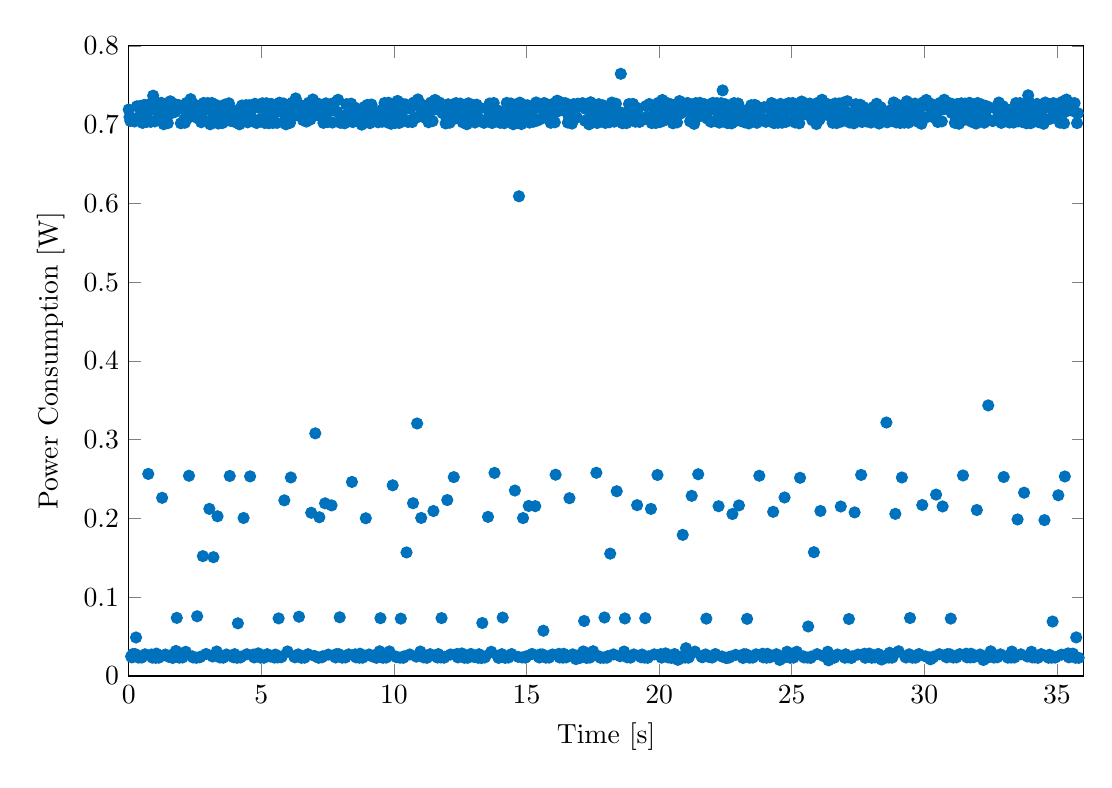
\begin{tikzpicture}

\begin{axis}[%
width=\textwidth,
height=0.66\textwidth,
at={(0.758in,0.481in)},
scale only axis,
xmin=0,
xmax=36,
ymin=0,
ymax=0.8,
xlabel={Time [s]},
ylabel={Power Consumption [W]},
axis background/.style={fill=white}
]
\addplot [color=mycolor1,only marks,mark=*,mark options={solid},forget plot]
  table[row sep=crcr]{%
0	0.719055\\
0.03072	0.70951068\\
0.06144	0.70463556\\
0.09216	0.0247879044\\
0.12288	0.0235748268\\
0.1536	0.0277404768\\
0.18432	0.7072218\\
0.21504	0.703926\\
0.24576	0.0277633656\\
0.27648	0.048843396\\
0.3072	0.72319788\\
0.33792	0.7089156\\
0.36864	0.023300172\\
0.39936	0.0246963492\\
0.43008	0.72358704\\
0.4608	0.72303768\\
0.49152	0.023345946\\
0.52224	0.70211772\\
0.55296	0.70761096\\
0.58368	0.72496044\\
0.6144	0.0274887072\\
0.64512	0.7139052\\
0.67584	0.70339968\\
0.70656	0.70806888\\
0.73728	0.256484988\\
0.768	0.72571572\\
0.79872	0.7208406\\
0.82944	0.7034454\\
0.86016	0.0271911636\\
0.89088	0.0232543944\\
0.9216	0.73672488\\
0.95232	0.71871192\\
0.98304	0.70399476\\
1.01376	0.0230483988\\
1.04448	0.02835846\\
1.0752	0.72752364\\
1.10592	0.7196274\\
1.13664	0.0232086168\\
1.16736	0.024765012\\
1.19808	0.7135848\\
1.2288	0.72756972\\
1.25952	0.22613526\\
1.29024	0.70930476\\
1.32096	0.70044696\\
1.35168	0.7126236\\
1.3824	0.0271911636\\
1.41312	0.72452556\\
1.44384	0.71186832\\
1.47456	0.70182036\\
1.50528	0.0243759168\\
1.536	0.72241956\\
1.56672	0.72956088\\
1.59744	0.71424864\\
1.62816	0.024765012\\
1.65888	0.0228652956\\
1.6896	0.0276260364\\
1.72032	0.72624204\\
1.75104	0.71610264\\
1.78176	0.0317001348\\
1.81248	0.073722852\\
1.8432	0.72035964\\
1.87392	0.72489168\\
1.90464	0.0232315056\\
1.93536	0.024879456\\
1.96608	0.7016832\\
1.9968	0.71997084\\
2.02752	0.0234146124\\
2.05824	0.7214814\\
2.08896	0.70598592\\
2.11968	0.70236972\\
2.1504	0.030670164\\
2.18112	0.72752364\\
2.21184	0.72230544\\
2.24256	0.70877844\\
2.27328	0.254150388\\
2.304	0.70992288\\
2.33472	0.73228464\\
2.36544	0.72468576\\
2.39616	0.0248565672\\
2.42688	0.0234603864\\
2.4576	0.71939844\\
2.48832	0.72473148\\
2.51904	0.72486864\\
2.54976	0.0230712876\\
2.58048	0.075759876\\
2.6112	0.70783992\\
2.64192	0.72049716\\
2.67264	0.0236206044\\
2.70336	0.024398802\\
2.73408	0.70298784\\
2.7648	0.7059402\\
2.79552	0.152114868\\
2.82624	0.72740952\\
2.85696	0.7179336\\
2.88768	0.70479576\\
2.9184	0.0279006948\\
2.94912	0.71951292\\
2.97984	0.727272\\
3.01056	0.72008532\\
3.04128	0.2121048\\
3.072	0.70040124\\
3.10272	0.72111528\\
3.13344	0.72745524\\
3.16416	0.0246963492\\
3.19488	0.150764472\\
3.2256	0.71168508\\
3.25632	0.7126236\\
3.28704	0.7249374\\
3.31776	0.0310363776\\
3.34848	0.202720644\\
3.3792	0.70133976\\
3.40992	0.7067412\\
3.44064	0.0234603864\\
3.47136	0.0250625628\\
3.50208	0.71395092\\
3.5328	0.70193484\\
3.56352	0.0231628392\\
3.59424	0.72280872\\
3.62496	0.72534924\\
3.65568	0.71582796\\
3.6864	0.0272140488\\
3.71712	0.70555104\\
3.74784	0.72054288\\
3.77856	0.72699732\\
3.80928	0.253898604\\
3.84	0.704727\\
3.87072	0.70909884\\
3.90144	0.71880336\\
3.93216	0.0241699212\\
3.96288	0.0236206044\\
3.9936	0.027671814\\
4.02432	0.70298784\\
4.05504	0.71768196\\
4.08576	0.0230941764\\
4.11648	0.0668106\\
4.1472	0.70822908\\
4.17792	0.70033248\\
4.20864	0.0234603864\\
4.23936	0.02455902\\
4.27008	0.72427356\\
4.3008	0.71099856\\
4.33152	0.200546244\\
4.36224	0.71024328\\
4.39296	0.72207648\\
4.42368	0.72463968\\
4.4544	0.0275344848\\
4.48512	0.70285032\\
4.51584	0.70820604\\
4.54656	0.72452556\\
4.57728	0.253372176\\
4.608	0.71699508\\
4.63872	0.70783992\\
4.66944	0.70564284\\
4.70016	0.0271224972\\
4.73088	0.023506164\\
4.7616	0.7263792\\
4.79232	0.70461288\\
4.82304	0.70202628\\
4.85376	0.0274200444\\
4.88448	0.0286560036\\
4.9152	0.72120672\\
4.94592	0.70662672\\
4.97664	0.023185728\\
5.00736	0.0247879044\\
5.03808	0.72702036\\
5.0688	0.72207648\\
5.09952	0.0231170652\\
5.13024	0.702072\\
5.16096	0.70925904\\
5.19168	0.72706608\\
5.2224	0.0276260364\\
5.25312	0.71257788\\
5.28384	0.70170588\\
5.31456	0.7122114\\
5.34528	0.0246734604\\
5.376	0.726219\\
5.40672	0.7179336\\
5.43744	0.702072\\
5.46816	0.0249481188\\
5.49888	0.0233230572\\
5.5296	0.0271224972\\
5.56032	0.71582796\\
5.59104	0.70214076\\
5.62176	0.023506164\\
5.65248	0.07308198\\
5.6832	0.72779832\\
5.71392	0.71804808\\
5.74464	0.0237579336\\
5.77536	0.0247879044\\
5.80608	0.7186662\\
5.8368	0.72674568\\
5.86752	0.2229309\\
5.89824	0.70664976\\
5.92896	0.7003098\\
5.95968	0.71710956\\
5.9904	0.0311050404\\
6.02112	0.72328932\\
6.05184	0.70854948\\
6.08256	0.70220952\\
6.11328	0.251975988\\
6.144	0.72560124\\
6.17472	0.72800424\\
6.20544	0.71056368\\
6.23616	0.0246963492\\
6.26688	0.0236434932\\
6.2976	0.73320012\\
6.32832	0.72553248\\
6.35904	0.71314992\\
6.38976	0.0273971556\\
6.42048	0.075187692\\
6.4512	0.72351828\\
6.48192	0.72468576\\
6.51264	0.0230712876\\
6.54336	0.0249481188\\
6.57408	0.7056198\\
6.6048	0.7210008\\
6.63552	0.0232315056\\
6.66624	0.71813952\\
6.69696	0.70378884\\
6.72768	0.70493328\\
6.7584	0.0275802588\\
6.78912	0.72770688\\
6.81984	0.71990208\\
6.85056	0.70644384\\
6.88128	0.207183816\\
6.912	0.714798\\
6.94272	0.73191816\\
6.97344	0.72251136\\
7.00416	0.025451658\\
7.03488	0.307983384\\
7.0656	0.72173304\\
7.09632	0.72720324\\
7.12704	0.7244568\\
7.15776	0.0230483988\\
7.18848	0.201484656\\
7.2192	0.71070084\\
7.24992	0.72095472\\
7.28064	0.0236434932\\
7.31136	0.0249481188\\
7.34208	0.70218648\\
7.3728	0.70774848\\
7.40352	0.21913146\\
7.43424	0.7269516\\
7.46496	0.71580492\\
7.49568	0.70319376\\
7.5264	0.0270996084\\
7.55712	0.72118368\\
7.58784	0.72528084\\
7.61856	0.71754444\\
7.64928	0.216545112\\
7.68	0.70259868\\
7.71072	0.72450252\\
7.74144	0.7275924\\
7.77216	0.0246734604\\
7.80288	0.0234603864\\
7.8336	0.027717588\\
7.86432	0.71630856\\
7.89504	0.7314606\\
7.92576	0.0276031512\\
7.95648	0.074478132\\
7.9872	0.70220952\\
8.01792	0.70941924\\
8.04864	0.0232086168\\
8.07936	0.0245819088\\
8.11008	0.7115706\\
8.1408	0.70161444\\
8.17152	0.0234603864\\
8.20224	0.72576144\\
8.23296	0.72567\\
8.26368	0.712944\\
8.2944	0.0274200444\\
8.32512	0.70758828\\
8.35584	0.72157284\\
8.38656	0.72656244\\
8.41728	0.24632262\\
8.448	0.70314768\\
8.47872	0.71143344\\
8.50944	0.72191628\\
8.54016	0.0274200444\\
8.57088	0.0236206044\\
8.6016	0.71049492\\
8.63232	0.70447536\\
8.66304	0.71864316\\
8.69376	0.0231628428\\
8.72448	0.0282211308\\
8.7552	0.70616916\\
8.78592	0.6998976\\
8.81664	0.023185728\\
8.84736	0.0244903536\\
8.87808	0.7222824\\
8.9088	0.70834356\\
8.93952	0.200180052\\
8.97024	0.71456904\\
9.00096	0.72502884\\
9.03168	0.7232436\\
9.0624	0.0272827152\\
9.09312	0.7017516\\
9.12384	0.70802316\\
9.15456	0.72544104\\
9.18528	0.024765012\\
9.216	0.71379072\\
9.24672	0.70687872\\
9.27744	0.70898436\\
9.30816	0.0249481188\\
9.33888	0.0230026248\\
9.3696	0.0277404768\\
9.40032	0.70289604\\
9.43104	0.70630632\\
9.46176	0.0312881472\\
9.49248	0.073333728\\
9.5232	0.71832276\\
9.55392	0.7036056\\
9.58464	0.0230941764\\
9.61536	0.0246047976\\
9.64608	0.72738648\\
9.6768	0.71953596\\
9.70752	0.0233230572\\
9.73824	0.70301052\\
9.76896	0.71477496\\
9.79968	0.72770688\\
9.8304	0.0311050404\\
9.86112	0.70864092\\
9.89184	0.70099632\\
9.92256	0.71392824\\
9.95328	0.242042544\\
9.984	0.72436536\\
10.01472	0.71523288\\
10.04544	0.702072\\
10.07616	0.0245819088\\
10.10688	0.0238037112\\
10.1376	0.73001844\\
10.16832	0.71285256\\
10.19904	0.70209504\\
10.22976	0.0232086168\\
10.26048	0.07278444\\
10.2912	0.72667692\\
10.32192	0.71589672\\
10.35264	0.0230483988\\
10.38336	0.0249023412\\
10.41408	0.72159588\\
10.4448	0.7255782\\
10.47552	0.156806928\\
10.50624	0.70388028\\
10.53696	0.70339968\\
10.56768	0.72077184\\
10.5984	0.0272598264\\
10.62912	0.721161\\
10.65984	0.70603164\\
10.69056	0.70319376\\
10.72128	0.219314592\\
10.752	0.72809604\\
10.78272	0.72596736\\
10.81344	0.70841232\\
10.84416	0.0245361312\\
10.87488	0.320503212\\
10.9056	0.7319412\\
10.93632	0.7239762\\
10.96704	0.7107696\\
10.99776	0.0309677112\\
11.02848	0.200592036\\
11.0592	0.72521208\\
11.08992	0.72447984\\
11.12064	0.0235519416\\
11.15136	0.0249938964\\
11.18208	0.70841232\\
11.2128	0.72093204\\
11.24352	0.0230255136\\
11.27424	0.71589672\\
11.30496	0.7029648\\
11.33568	0.70724484\\
11.3664	0.0276260364\\
11.39712	0.72798156\\
11.42784	0.71795664\\
11.45856	0.70442964\\
11.48928	0.209381112\\
11.52	0.71992476\\
11.55072	0.73125468\\
11.58144	0.71948988\\
11.61216	0.0243301392\\
11.64288	0.0233917236\\
11.6736	0.027717588\\
11.70432	0.72814176\\
11.73504	0.72708876\\
11.76576	0.0234603864\\
11.79648	0.073448172\\
11.8272	0.71468352\\
11.85792	0.72393048\\
11.88864	0.0231628428\\
11.91936	0.0242843616\\
11.95008	0.70147692\\
11.9808	0.70832052\\
12.01152	0.223319988\\
12.04224	0.7257384\\
12.07296	0.71376804\\
12.10368	0.70234668\\
12.1344	0.0272369376\\
12.16512	0.72351828\\
12.19584	0.72473148\\
12.22656	0.71443188\\
12.25728	0.252433764\\
12.288	0.70738236\\
12.31872	0.72669996\\
12.34944	0.72718056\\
12.38016	0.0279006948\\
12.41088	0.0235519416\\
12.4416	0.71026596\\
12.47232	0.72081756\\
12.50304	0.72665388\\
12.53376	0.027465822\\
12.56448	0.028564452\\
12.5952	0.70285032\\
12.62592	0.71443188\\
12.65664	0.0231170652\\
12.68736	0.0246047976\\
12.71808	0.70854948\\
12.7488	0.70044696\\
12.77952	0.0230712876\\
12.81024	0.72704304\\
12.84096	0.72374724\\
12.87168	0.71038044\\
12.9024	0.0279464724\\
12.93312	0.7109298\\
12.96384	0.72280872\\
12.99456	0.72452556\\
13.02528	0.0241012584\\
13.056	0.7026444\\
13.08672	0.71353908\\
13.11744	0.72530352\\
13.14816	0.025085448\\
13.17888	0.0230712876\\
13.2096	0.02755737\\
13.24032	0.706833\\
13.27104	0.72086328\\
13.30176	0.022819518\\
13.33248	0.067222584\\
13.3632	0.70397172\\
13.39392	0.7022322\\
13.42464	0.0234375012\\
13.45536	0.0250167852\\
13.48608	0.7208406\\
13.5168	0.70557408\\
13.54752	0.201965328\\
13.57824	0.71710956\\
13.60896	0.72674568\\
13.63968	0.7213896\\
13.6704	0.030670164\\
13.70112	0.70198056\\
13.73184	0.71017452\\
13.76256	0.72738648\\
13.79328	0.257766732\\
13.824	0.71179956\\
13.85472	0.70664976\\
13.88544	0.71216568\\
13.91616	0.0249252336\\
13.94688	0.0229339584\\
13.9776	0.71710956\\
14.00832	0.70225524\\
14.03904	0.708435\\
14.06976	0.0276489252\\
14.10048	0.07411194\\
14.1312	0.7152786\\
14.16192	0.70177464\\
14.19264	0.0230255136\\
14.22336	0.02455902\\
14.25408	0.72754668\\
14.2848	0.71747604\\
14.31552	0.0233230572\\
14.34624	0.70461288\\
14.37696	0.7202682\\
14.40768	0.72681444\\
14.4384	0.0277862544\\
14.46912	0.70623792\\
14.49984	0.70042428\\
14.53056	0.7172928\\
14.56128	0.235404972\\
14.592	0.72315216\\
14.62272	0.71280684\\
14.65344	0.70209504\\
14.68416	0.0242385876\\
14.71488	0.60896304\\
14.7456	0.72782136\\
14.77632	0.70946496\\
14.80704	0.70069896\\
14.83776	0.0234603864\\
14.86848	0.200431836\\
14.8992	0.72496044\\
14.92992	0.71255484\\
14.96064	0.0232086168\\
14.99136	0.0249481188\\
15.02208	0.72425088\\
15.0528	0.72431928\\
15.08352	0.215835552\\
15.11424	0.70250688\\
15.14496	0.70687872\\
15.17568	0.72168732\\
15.2064	0.0279235836\\
15.23712	0.7179336\\
15.26784	0.70362864\\
15.29856	0.70573428\\
15.32928	0.215560908\\
15.36	0.72809604\\
15.39072	0.7234038\\
15.42144	0.70523064\\
15.45216	0.0245361312\\
15.48288	0.0233917236\\
15.5136	0.0273284928\\
15.54432	0.72068004\\
15.57504	0.70777116\\
15.60576	0.0272827152\\
15.63648	0.057403548\\
15.6672	0.72738648\\
15.69792	0.72354132\\
15.72864	0.0232543944\\
15.75936	0.0247879044\\
15.79008	0.71168508\\
15.8208	0.72198468\\
15.85152	0.0232772832\\
15.88224	0.71179956\\
15.91296	0.70225524\\
15.94368	0.70829784\\
15.9744	0.0272369376\\
16.00512	0.72651672\\
16.03584	0.71472924\\
16.06656	0.70282728\\
16.09728	0.255477888\\
16.128	0.72184752\\
16.15872	0.73036188\\
16.18944	0.71690364\\
16.22016	0.028038024\\
16.25088	0.0234603864\\
16.2816	0.72821052\\
16.31232	0.72754668\\
16.34304	0.71990208\\
16.37376	0.0232315056\\
16.40448	0.0280838016\\
16.4352	0.71781912\\
16.46592	0.72720324\\
16.49664	0.0235519416\\
16.52736	0.0249252336\\
16.55808	0.70250688\\
16.5888	0.71065512\\
16.61952	0.225654588\\
16.65024	0.7239762\\
16.68096	0.71056368\\
16.71168	0.701271\\
16.7424	0.0273971556\\
16.77312	0.72594432\\
16.80384	0.72500616\\
16.83456	0.71191404\\
16.86528	0.0213775596\\
16.896	0.7090758\\
16.92672	0.7263792\\
16.95744	0.72596736\\
16.98816	0.0248107896\\
17.01888	0.0229568472\\
17.0496	0.0274429296\\
17.08032	0.72301464\\
17.11104	0.72720324\\
17.14176	0.0310821516\\
17.17248	0.069786072\\
17.2032	0.70486452\\
17.23392	0.71990208\\
17.26464	0.0229110696\\
17.29536	0.0249938964\\
17.32608	0.70600896\\
17.3568	0.70033248\\
17.38752	0.0232772832\\
17.41824	0.72830196\\
17.44896	0.7218018\\
17.47968	0.70724484\\
17.5104	0.0313796988\\
17.54112	0.71445456\\
17.57184	0.72505188\\
17.60256	0.72219096\\
17.63328	0.257926932\\
17.664	0.70198056\\
17.69472	0.71385948\\
17.72544	0.7258986\\
17.75616	0.0246505752\\
17.78688	0.0230941764\\
17.8176	0.70724484\\
17.84832	0.70944228\\
17.87904	0.72443376\\
17.90976	0.0230483988\\
17.94048	0.074226384\\
17.9712	0.70211772\\
18.00192	0.7066728\\
18.03264	0.0232086168\\
18.06336	0.0251541144\\
18.09408	0.71756748\\
18.1248	0.70291908\\
18.15552	0.155273436\\
18.18624	0.72051984\\
18.21696	0.7279128\\
18.24768	0.7183458\\
18.2784	0.0273742668\\
18.30912	0.70372008\\
18.33984	0.71530164\\
18.37056	0.72656244\\
18.40128	0.234489456\\
18.432	0.70783992\\
18.46272	0.70536816\\
18.49344	0.71530164\\
18.52416	0.0250625628\\
18.55488	0.7644654\\
18.5856	0.71498124\\
18.61632	0.70172892\\
18.64704	0.71234892\\
18.67776	0.0309677112\\
18.70848	0.072990432\\
18.7392	0.71218872\\
18.76992	0.7018434\\
18.80064	0.0236206044\\
18.83136	0.0246963492\\
18.86208	0.72603612\\
18.8928	0.7142256\\
18.92352	0.0232543944\\
18.95424	0.70662672\\
18.98496	0.72177876\\
19.01568	0.72626508\\
19.0464	0.0273056004\\
19.07712	0.7042464\\
19.10784	0.70369704\\
19.13856	0.72168732\\
19.16928	0.216819756\\
19.2	0.71981064\\
19.23072	0.70909884\\
19.26144	0.70337664\\
19.29216	0.0249252336\\
19.32288	0.0237350448\\
19.3536	0.0271682712\\
19.38432	0.7067412\\
19.41504	0.70655832\\
19.44576	0.0232772832\\
19.47648	0.07337952\\
19.5072	0.72354132\\
19.53792	0.70983108\\
19.56864	0.0230026248\\
19.59936	0.024879456\\
19.63008	0.72610488\\
19.6608	0.72431928\\
19.69152	0.212081904\\
19.72224	0.7019118\\
19.75296	0.7095564\\
19.78368	0.72152712\\
19.8144	0.0273971556\\
19.84512	0.71456904\\
19.87584	0.70202628\\
19.90656	0.70770276\\
19.93728	0.255157488\\
19.968	0.7275924\\
19.99872	0.72177876\\
20.02944	0.703125\\
20.06016	0.0276489252\\
20.09088	0.0232543944\\
20.1216	0.73118592\\
20.15232	0.71852868\\
20.18304	0.7051392\\
20.21376	0.0277404768\\
20.24448	0.0286331184\\
20.2752	0.72770688\\
20.30592	0.72150408\\
20.33664	0.023506164\\
20.36736	0.024719238\\
20.39808	0.71587368\\
20.4288	0.72594432\\
20.45952	0.0228881844\\
20.49024	0.70935048\\
20.52096	0.70163712\\
20.55168	0.70930476\\
20.5824	0.0277633656\\
20.61312	0.72518904\\
20.64384	0.71253216\\
20.67456	0.70273584\\
20.70528	0.0204391476\\
20.736	0.72454824\\
20.76672	0.72983556\\
20.79744	0.71385948\\
20.82816	0.0246734604\\
20.85888	0.0230712876\\
20.8896	0.179122932\\
20.92032	0.7269516\\
20.95104	0.71674344\\
20.98176	0.023300172\\
21.01248	0.0352249128\\
21.0432	0.72072612\\
21.07392	0.72740952\\
21.10464	0.0232086168\\
21.13536	0.024719238\\
21.16608	0.7040862\\
21.1968	0.7160112\\
21.22752	0.228652956\\
21.25824	0.72113796\\
21.28896	0.7073136\\
21.31968	0.70090488\\
21.3504	0.0308990484\\
21.38112	0.72724896\\
21.41184	0.72377028\\
21.44256	0.70925904\\
21.47328	0.256073004\\
21.504	0.71207424\\
21.53472	0.7275924\\
21.56544	0.72443376\\
21.59616	0.024765012\\
21.62688	0.0236892708\\
21.6576	0.71466048\\
21.68832	0.72518904\\
21.71904	0.72576144\\
21.74976	0.0273284928\\
21.78048	0.07278444\\
21.8112	0.70758828\\
21.84192	0.72191628\\
21.87264	0.0241241436\\
21.90336	0.0246963492\\
21.93408	0.70436088\\
21.9648	0.70337664\\
21.99552	0.023345946\\
22.02624	0.7275924\\
22.05696	0.7192152\\
22.08768	0.70458984\\
22.1184	0.0277862544\\
22.14912	0.7185744\\
22.17984	0.72718056\\
22.21056	0.72049716\\
22.24128	0.215492256\\
22.272	0.70243848\\
22.30272	0.71594244\\
22.33344	0.72718056\\
22.36416	0.0247421268\\
22.39488	0.74338524\\
22.4256	0.7066728\\
22.45632	0.71344764\\
22.48704	0.72592164\\
22.51776	0.022979736\\
22.54848	0.022819518\\
22.5792	0.70188912\\
22.60992	0.70930476\\
22.64064	0.0233230572\\
22.67136	0.024513246\\
22.70208	0.7136766\\
22.7328	0.70149996\\
22.76352	0.205558776\\
22.79424	0.72290052\\
22.82496	0.727272\\
22.85568	0.71658324\\
22.8864	0.026779176\\
22.91712	0.70502472\\
22.94784	0.72008532\\
22.97856	0.7267914\\
23.00928	0.21649932\\
23.04	0.70568856\\
23.07072	0.70475004\\
23.10144	0.71912376\\
23.13216	0.0247879044\\
23.16288	0.0227966292\\
23.1936	0.0276031512\\
23.22432	0.70282728\\
23.25504	0.71569044\\
23.28576	0.0274200444\\
23.31648	0.072486864\\
23.3472	0.70971696\\
23.37792	0.7014312\\
23.40864	0.023185728\\
23.43936	0.024513246\\
23.47008	0.72454824\\
23.5008	0.71170812\\
23.53152	0.023300172\\
23.56224	0.70978536\\
23.59296	0.72482292\\
23.62368	0.72466272\\
23.6544	0.0274429296\\
23.68512	0.70225524\\
23.71584	0.70717608\\
23.74656	0.72198468\\
23.77728	0.254173248\\
23.808	0.71733852\\
23.83872	0.70774848\\
23.86944	0.70607772\\
23.90016	0.0281524644\\
23.93088	0.0235519416\\
23.9616	0.72209916\\
23.99232	0.70509348\\
24.02304	0.70349112\\
24.05376	0.023139954\\
24.08448	0.028038024\\
24.1152	0.72040572\\
24.14592	0.70726788\\
24.17664	0.0236434932\\
24.20736	0.0248107896\\
24.23808	0.72734076\\
24.2688	0.72331236\\
24.29952	0.208374012\\
24.33024	0.70186608\\
24.36096	0.71335584\\
24.39168	0.72239688\\
24.4224	0.0276260364\\
24.45312	0.711891\\
24.48384	0.70227828\\
24.51456	0.7098084\\
24.54528	0.020347596\\
24.576	0.72628776\\
24.60672	0.71884908\\
24.63744	0.7023924\\
24.66816	0.024353028\\
24.69888	0.0232086168\\
24.7296	0.226570104\\
24.76032	0.71589672\\
24.79104	0.70353684\\
24.82176	0.0306930528\\
24.85248	0.0293884272\\
24.8832	0.72722628\\
24.91392	0.71955864\\
24.94464	0.0230483988\\
24.97536	0.0249938964\\
25.00608	0.7191468\\
25.0368	0.72738648\\
25.06752	0.0232543944\\
25.09824	0.70648956\\
25.12896	0.7026444\\
25.15968	0.71115876\\
25.1904	0.0306930528\\
25.22112	0.7226028\\
25.25184	0.70960248\\
25.28256	0.70163712\\
25.31328	0.251564004\\
25.344	0.72681444\\
25.37472	0.72926316\\
25.40544	0.7122114\\
25.43616	0.0249023412\\
25.46688	0.0234603864\\
25.4976	0.72683712\\
25.52832	0.72473148\\
25.55904	0.71381376\\
25.58976	0.023300172\\
25.62048	0.062828064\\
25.6512	0.72351828\\
25.68192	0.72665388\\
25.71264	0.0229110696\\
25.74336	0.0246505752\\
25.77408	0.70559676\\
25.8048	0.72072612\\
25.83552	0.157081608\\
25.86624	0.71818524\\
25.89696	0.70438392\\
25.92768	0.70065324\\
25.9584	0.0276947028\\
25.98912	0.7277526\\
26.01984	0.721161\\
26.05056	0.70644384\\
26.08128	0.209426868\\
26.112	0.71580492\\
26.14272	0.7314606\\
26.17344	0.72200772\\
26.20416	0.0250396704\\
26.23488	0.72715752\\
26.2656	0.7146378\\
26.29632	0.7266312\\
26.32704	0.72475416\\
26.35776	0.0307388304\\
26.38848	0.0198211644\\
26.4192	0.71113572\\
26.44992	0.72496044\\
26.48064	0.0231628428\\
26.51136	0.0246734604\\
26.54208	0.70225524\\
26.5728	0.70804584\\
26.60352	0.023139954\\
26.63424	0.72683712\\
26.66496	0.71651448\\
26.69568	0.7019118\\
26.7264	0.0272369376\\
26.75712	0.72070308\\
26.78784	0.72683712\\
26.81856	0.71752176\\
26.84928	0.215126028\\
26.88	0.70399476\\
26.91072	0.72045144\\
26.94144	0.72772992\\
26.97216	0.0249938964\\
27.00288	0.0231628428\\
27.0336	0.027511596\\
27.06432	0.71596512\\
27.09504	0.72967536\\
27.12576	0.023666382\\
27.15648	0.072280872\\
27.1872	0.70259868\\
27.21792	0.71289828\\
27.24864	0.0227966292\\
27.27936	0.0249023412\\
27.31008	0.71095284\\
27.3408	0.70156872\\
27.37152	0.207618696\\
27.40224	0.72564696\\
27.43296	0.72560124\\
27.46368	0.71337888\\
27.4944	0.0271682712\\
27.52512	0.70800012\\
27.55584	0.72235116\\
27.58656	0.72512064\\
27.61728	0.25522614\\
27.648	0.70326216\\
27.67872	0.70912152\\
27.70944	0.72216792\\
27.74016	0.0281524644\\
27.77088	0.0230712876\\
27.8016	0.70896132\\
27.83232	0.70390332\\
27.86304	0.71836848\\
27.89376	0.027465822\\
27.92448	0.0283813452\\
27.9552	0.70639812\\
27.98592	0.7025526\\
28.01664	0.0230941764\\
28.04736	0.0244445796\\
28.07808	0.72225936\\
28.1088	0.70832052\\
28.13952	0.0235519416\\
28.17024	0.71452332\\
28.20096	0.72642528\\
28.23168	0.723564\\
28.2624	0.0279006948\\
28.29312	0.70129404\\
28.32384	0.71003736\\
28.35456	0.72203076\\
28.38528	0.0208282464\\
28.416	0.71376804\\
28.44672	0.70582572\\
28.47744	0.7085952\\
28.50816	0.0251541144\\
28.53888	0.0232086168\\
28.5696	0.321739164\\
28.60032	0.70285032\\
28.63104	0.70534512\\
28.66176	0.0232772832\\
28.69248	0.0294113124\\
28.7232	0.71813952\\
28.75392	0.70493328\\
28.78464	0.0232086168\\
28.81536	0.0247421268\\
28.84608	0.72809604\\
28.8768	0.72081756\\
28.90752	0.205764768\\
28.93824	0.70275888\\
28.96896	0.71644608\\
28.99968	0.7250976\\
29.0304	0.0313339212\\
29.06112	0.7090758\\
29.09184	0.70202628\\
29.12256	0.7107696\\
29.15328	0.251953128\\
29.184	0.72452556\\
29.21472	0.71610264\\
29.24544	0.70241544\\
29.27616	0.0246047976\\
29.30688	0.0233917236\\
29.3376	0.72956088\\
29.36832	0.71301276\\
29.39904	0.7023924\\
29.42976	0.027511596\\
29.46048	0.073562616\\
29.4912	0.72612756\\
29.52192	0.7159194\\
29.55264	0.0231628428\\
29.58336	0.0246963492\\
29.61408	0.72166428\\
29.6448	0.7266312\\
29.67552	0.0232543944\\
29.70624	0.70426944\\
29.73696	0.70454412\\
29.76768	0.71571348\\
29.7984	0.027832032\\
29.82912	0.72061164\\
29.85984	0.70664976\\
29.89056	0.70099632\\
29.92128	0.217002852\\
29.952	0.7281648\\
29.98272	0.72789012\\
30.01344	0.7085952\\
30.04416	0.024879456\\
30.07488	0.73123164\\
30.1056	0.72841644\\
30.13632	0.72351828\\
30.16704	0.7104492\\
30.19776	0.0234374976\\
30.22848	0.0211029048\\
30.2592	0.72617328\\
30.28992	0.72523512\\
30.32064	0.0232772832\\
30.35136	0.0246963492\\
30.38208	0.70866396\\
30.4128	0.72198468\\
30.44352	0.23023224\\
30.47424	0.71598816\\
30.50496	0.7032852\\
30.53568	0.70394904\\
30.5664	0.0275802588\\
30.59712	0.72763812\\
30.62784	0.71916948\\
30.65856	0.70404048\\
30.68928	0.215194716\\
30.72	0.71953596\\
30.75072	0.73148328\\
30.78144	0.72019944\\
30.81216	0.0246047976\\
30.84288	0.0235748268\\
30.8736	0.027717588\\
30.90432	0.72779832\\
30.93504	0.72187056\\
30.96576	0.027465822\\
30.99648	0.0728073\\
31.0272	0.71486676\\
31.05792	0.72601308\\
31.08864	0.023345946\\
31.11936	0.0246047976\\
31.15008	0.70218648\\
31.1808	0.71022024\\
31.21152	0.0235748268\\
31.24224	0.72610488\\
31.27296	0.71335584\\
31.30368	0.70104204\\
31.3344	0.027717588\\
31.36512	0.723816\\
31.39584	0.72702036\\
31.42656	0.71523288\\
31.45728	0.254539476\\
31.488	0.70598592\\
31.51872	0.7263108\\
31.54944	0.72658548\\
31.58016	0.0282211308\\
31.61088	0.0235748268\\
31.6416	0.70591752\\
31.67232	0.72013104\\
31.70304	0.72763812\\
31.73376	0.0235290528\\
31.76448	0.0281753532\\
31.7952	0.70339968\\
31.82592	0.7160112\\
31.85664	0.0237350448\\
31.88736	0.0250167852\\
31.91808	0.70802316\\
31.9488	0.701271\\
31.97952	0.210662856\\
32.01024	0.72736344\\
32.04096	0.724617\\
32.07168	0.71120448\\
32.1024	0.0271911636\\
32.13312	0.71099856\\
32.16384	0.72528084\\
32.19456	0.72436536\\
32.22528	0.0202560408\\
32.256	0.70236972\\
32.28672	0.7135848\\
32.31744	0.7237242\\
32.34816	0.0249023412\\
32.37888	0.023185728\\
32.4096	0.343482948\\
32.44032	0.70603164\\
32.47104	0.72152712\\
32.50176	0.0312423696\\
32.53248	0.0292739832\\
32.5632	0.7046586\\
32.59392	0.70463556\\
32.62464	0.0233230572\\
32.65536	0.0243759168\\
32.68608	0.72051984\\
32.7168	0.7063524\\
32.74752	0.0236434932\\
32.77824	0.71651448\\
32.80896	0.72798156\\
32.83968	0.72221364\\
32.8704	0.0274429296\\
32.90112	0.7021638\\
32.93184	0.71417988\\
32.96256	0.72331236\\
32.99328	0.252571104\\
33.024	0.71056368\\
33.05472	0.7062606\\
33.08544	0.71063244\\
33.11616	0.025085448\\
33.14688	0.0232315056\\
33.1776	0.7186662\\
33.20832	0.70259868\\
33.23904	0.70866396\\
33.26976	0.0233230572\\
33.30048	0.0309219336\\
33.3312	0.7151184\\
33.36192	0.7025526\\
33.39264	0.0234146124\\
33.42336	0.0251541144\\
33.45408	0.72724896\\
33.4848	0.71818524\\
33.51552	0.198692316\\
33.54624	0.70410924\\
33.57696	0.71951292\\
33.60768	0.727272\\
33.6384	0.0274887072\\
33.66912	0.70580304\\
33.69984	0.70321644\\
33.73056	0.711891\\
33.76128	0.232658388\\
33.792	0.72301464\\
33.82272	0.71335584\\
33.85344	0.70163712\\
33.88416	0.0246734604\\
33.91488	0.73720548\\
33.9456	0.72898848\\
33.97632	0.71081532\\
34.00704	0.70172892\\
34.03776	0.0306930528\\
34.06848	0.0235519416\\
34.0992	0.72521208\\
34.12992	0.71248608\\
34.16064	0.023506164\\
34.19136	0.0244445796\\
34.22208	0.72491436\\
34.2528	0.72624204\\
34.28352	0.0230255136\\
34.31424	0.70298784\\
34.34496	0.70630632\\
34.37568	0.72145836\\
34.4064	0.0276947028\\
34.43712	0.71781912\\
34.46784	0.70390332\\
34.49856	0.70101936\\
34.52928	0.197799696\\
34.56	0.72800424\\
34.59072	0.72521208\\
34.62144	0.70591752\\
34.65216	0.0244903536\\
34.68288	0.0231170652\\
34.7136	0.0268478388\\
34.74432	0.72065736\\
34.77504	0.70767972\\
34.80576	0.0232315056\\
34.83648	0.069099408\\
34.8672	0.72722628\\
34.89792	0.7231752\\
34.92864	0.0233230572\\
34.95936	0.0241470324\\
34.99008	0.7115022\\
35.0208	0.72546372\\
35.05152	0.229385376\\
35.08224	0.71241768\\
35.11296	0.7023924\\
35.14368	0.70880112\\
35.1744	0.027030942\\
35.20512	0.72898848\\
35.23584	0.7161714\\
35.26656	0.70161444\\
35.29728	0.253257732\\
35.328	0.72251136\\
35.35872	0.73175796\\
35.38944	0.7172928\\
35.42016	0.0286102296\\
35.45088	0.0235977156\\
35.4816	0.72141264\\
35.51232	0.72763812\\
35.54304	0.71955864\\
35.57376	0.0275344848\\
35.60448	0.0282897936\\
35.6352	0.71685792\\
35.66592	0.72720324\\
35.69664	0.023139954\\
35.72736	0.048912048\\
35.75808	0.70186608\\
35.7888	0.71440884\\
35.81952	0.0230255136\\
};
\end{axis}
\end{tikzpicture}%}
\caption{Example of raw measurements of the transmit case.}
\label{fig:Transmit_raw}
\end{figure}

As seen in \autoref{fig:Transmit_raw} the device is in a transmit state for the entirety of the measurement. The average power consumption is therefore calculated based on \autoref{eq:power} with the whole measurement being the area of interest. This is done for all parameters and the result can be seen in \autoref{fig:Transmit_Points}.

\begin{figure}[H]
\centering
\begin{minipage}{0.48\textwidth}
\tikzsetnextfilename{Transmit_Points}
\resizebox{\textwidth}{!}{
% This file was created by matlab2tikz.
%
%The latest updates can be retrieved from
%  http://www.mathworks.com/matlabcentral/fileexchange/22022-matlab2tikz-matlab2tikz
%where you can also make suggestions and rate matlab2tikz.
%
\definecolor{mycolor1}{rgb}{0.00000,0.44700,0.74100}%
\definecolor{mycolor2}{rgb}{0.85000,0.32500,0.09800}%
\definecolor{mycolor3}{rgb}{0.92900,0.69400,0.12500}%
\definecolor{mycolor4}{rgb}{0.49400,0.18400,0.55600}%
%
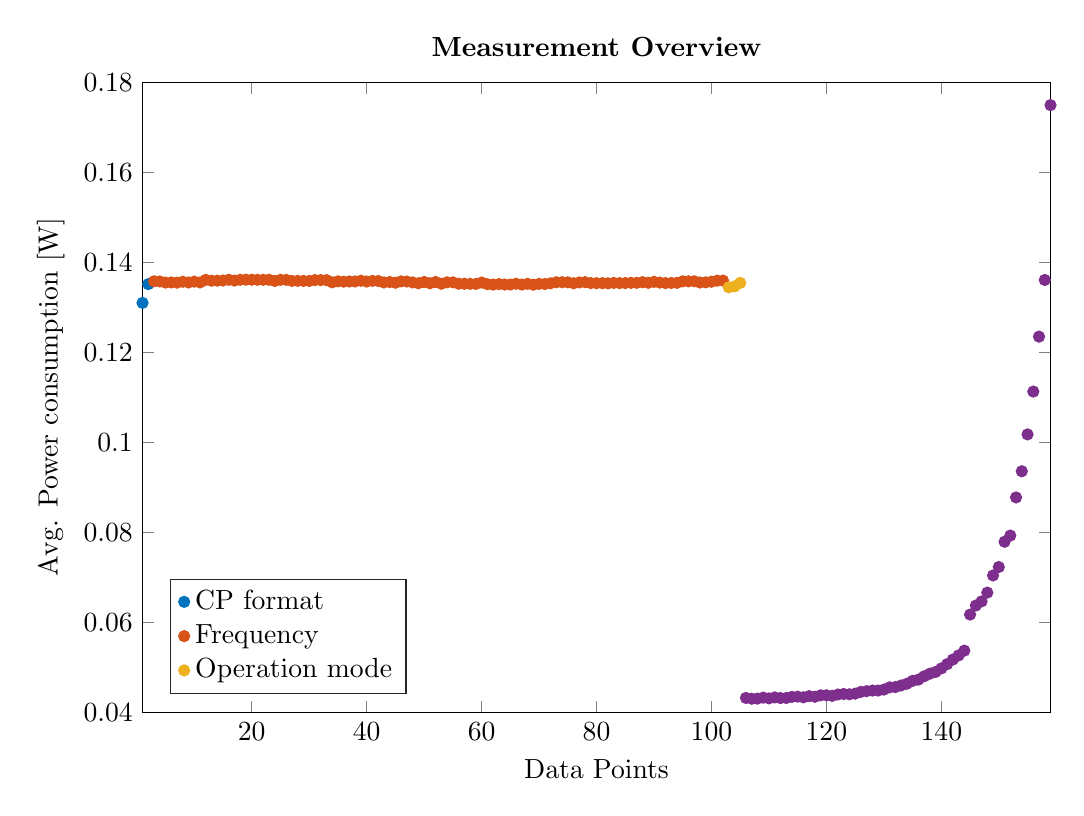
\begin{tikzpicture}

\begin{axis}[%
width=0.951\textwidth,
height=0.66\textwidth,
at={(0\textwidth,0\textwidth)},
scale only axis,
xmin=1,
xmax=159,
xlabel={Data Points},
ymin=0.04,
ymax=0.18,
ylabel={Avg. Power consumption [W]},
axis background/.style={fill=white},
title style={font=\bfseries},
title={Measurement Overview},
legend style={at={(0.03,0.03)},anchor=south west,legend cell align=left,align=left,draw=white!15!black},
y tick label style={/pgf/number format/fixed}
]
\addplot [color=mycolor1,only marks,mark=*,mark options={solid}]
  table[row sep=crcr]{%
1	0.131034879691784\\
2	0.135206269300117\\
};
\addlegendentry{CP format};

\addplot [color=mycolor2,only marks,mark=*,mark options={solid}]
  table[row sep=crcr]{%
3	0.135829821049459\\
4	0.135795684929074\\
5	0.135548569987852\\
6	0.135577564808571\\
7	0.135534178338524\\
8	0.135727405853401\\
9	0.135572171857743\\
10	0.13576021115347\\
11	0.135577925402099\\
12	0.136152962699817\\
13	0.135964314501334\\
14	0.135971211199521\\
15	0.136002139090922\\
16	0.136176454410933\\
17	0.1359879811862\\
18	0.136168580140498\\
19	0.136183723981932\\
20	0.136181740560122\\
21	0.13616678569156\\
22	0.136161475038809\\
23	0.136174058866293\\
24	0.135906947053042\\
25	0.13615405677175\\
26	0.136150442623051\\
27	0.135925289935805\\
28	0.135927153368611\\
29	0.13591955162778\\
30	0.135902203870294\\
31	0.136102630855924\\
32	0.136092075747546\\
33	0.136087729696951\\
34	0.13560293284348\\
35	0.135818827502946\\
36	0.135751801086845\\
37	0.1357953285655\\
38	0.135791248474108\\
39	0.135961356928112\\
40	0.135776763525742\\
41	0.135922330158771\\
42	0.13590407367665\\
43	0.135574757414205\\
44	0.135673077262854\\
45	0.135512156332663\\
46	0.135818839069838\\
47	0.135781754964222\\
48	0.135575646789595\\
49	0.135402692797852\\
50	0.13568474838069\\
51	0.135392093380107\\
52	0.135671437428649\\
53	0.135294028343203\\
54	0.135600166083035\\
55	0.135599444034098\\
56	0.135299883105007\\
57	0.135286355166246\\
58	0.135261102066647\\
59	0.135240394499234\\
60	0.135555665658007\\
61	0.13519196612858\\
62	0.135103591432874\\
63	0.135213524386535\\
64	0.135113598273484\\
65	0.135110539597205\\
66	0.135290143197378\\
67	0.135107973018762\\
68	0.135271780414257\\
69	0.135066044937166\\
70	0.135260596885485\\
71	0.135226596522249\\
72	0.135395855440633\\
73	0.135611631138825\\
74	0.135622955103172\\
75	0.135594409106628\\
76	0.135397213890925\\
77	0.135581507604902\\
78	0.135635085247642\\
79	0.135434263265754\\
80	0.135419162633024\\
81	0.135414966008461\\
82	0.135378056396111\\
83	0.135471137663363\\
84	0.13542695815948\\
85	0.135441789644027\\
86	0.135489011808238\\
87	0.135496424566135\\
88	0.135642494969293\\
89	0.135498924887968\\
90	0.135709610142296\\
91	0.135546033303295\\
92	0.135432140484162\\
93	0.135462030749248\\
94	0.135488953040129\\
95	0.135821924450509\\
96	0.135821571098135\\
97	0.1358277489622\\
98	0.135561639609378\\
99	0.135597077745581\\
100	0.135734557842914\\
101	0.135969635728828\\
102	0.135990533251521\\
};
\addlegendentry{Frequency};

\addplot [color=mycolor3,only marks,mark=*,mark options={solid}]
  table[row sep=crcr]{%
103	0.134506684862211\\
104	0.134697259444993\\
105	0.13547584703856\\
};
\addlegendentry{Operation mode};

\addplot [color=mycolor4,only marks,mark=*,mark options={solid},forget plot]
  table[row sep=crcr]{%
106	0.0432671370442985\\
107	0.0430935271540902\\
108	0.0431155547810735\\
109	0.0433332959821664\\
110	0.0431660444350098\\
111	0.0433854386156806\\
112	0.0432345150410041\\
113	0.0432525264618958\\
114	0.0434999814497639\\
115	0.0435548718544184\\
116	0.0434029278993332\\
117	0.0436726853298729\\
118	0.0435259843807757\\
119	0.0438432049965383\\
120	0.043861312456332\\
121	0.0437250232069267\\
122	0.0440310218032299\\
123	0.0441436351842956\\
124	0.0440716559725411\\
125	0.0442200313078414\\
126	0.0446109538683134\\
127	0.0447768047382843\\
128	0.0449036143685845\\
129	0.0449127933362612\\
130	0.045118962743008\\
131	0.0456148403706944\\
132	0.0456832887367053\\
133	0.0460319501445317\\
134	0.0464200132118457\\
135	0.0470602737490459\\
136	0.0473341788384111\\
137	0.0480683479919247\\
138	0.0486490752697266\\
139	0.0490368064453516\\
140	0.0498296655741014\\
141	0.0507689571429081\\
142	0.0517899366621504\\
143	0.0527056931949284\\
144	0.0537705239438872\\
145	0.0617877150990408\\
146	0.0637950254237825\\
147	0.064713243745866\\
148	0.0666659683567463\\
149	0.0704764637679604\\
150	0.0723517382545409\\
151	0.077964939639652\\
152	0.079334950628774\\
153	0.0878082519401085\\
154	0.0936253392352084\\
155	0.101816405487039\\
156	0.111331959596792\\
157	0.123535456484453\\
158	0.136128742064438\\
159	0.174972950689174\\
};
\addlegendentry{$P_{TX}$};
\end{axis}
\end{tikzpicture}%}
\end{minipage}
\hfill
\begin{minipage}{0.48\textwidth}
\tikzsetnextfilename{Transmit_Stat}
\resizebox{\textwidth}{!}{
% This file was created by matlab2tikz.
%
%The latest updates can be retrieved from
%  http://www.mathworks.com/matlabcentral/fileexchange/22022-matlab2tikz-matlab2tikz
%where you can also make suggestions and rate matlab2tikz.
%
\definecolor{mycolor1}{rgb}{0.00000,0.44700,0.74100}%
\definecolor{mycolor2}{rgb}{0.85000,0.32500,0.09800}%
%
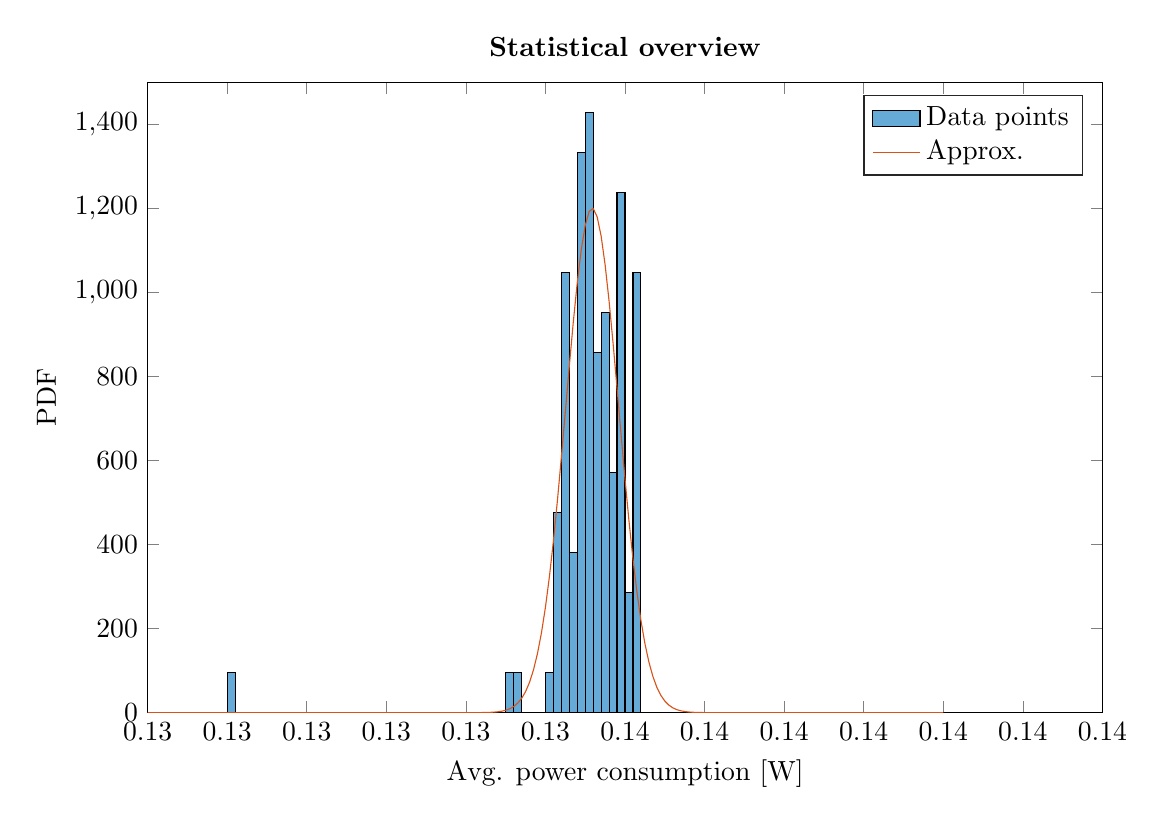
\begin{tikzpicture}

\begin{axis}[%
width=\textwidth,
height=0.66\textwidth,
at={(2.08in,0.858in)},
scale only axis,
xmin=0.13,
xmax=0.142,
xlabel={Avg. power consumption [W]},
ymin=0,
ymax=1500,
ylabel={PDF},
axis background/.style={fill=white},
title style={font=\bfseries},
title={Statistical overview},
legend style={legend cell align=left,align=left,draw=white!15!black}
]
\addplot[fill=mycolor1,fill opacity=0.6,draw=black,ybar interval,area legend] plot table[row sep=crcr] {%
x	y\\
0.131	95.2380952381057\\
0.1311	0\\
0.1312	0\\
0.1313	0\\
0.1314	0\\
0.1315	0\\
0.1316	0\\
0.1317	0\\
0.1318	0\\
0.1319	0\\
0.132	0\\
0.1321	0\\
0.1322	0\\
0.1323	0\\
0.1324	0\\
0.1325	0\\
0.1326	0\\
0.1327	0\\
0.1328	0\\
0.1329	0\\
0.133	0\\
0.1331	0\\
0.1332	0\\
0.1333	0\\
0.1334	0\\
0.1335	0\\
0.1336	0\\
0.1337	0\\
0.1338	0\\
0.1339	0\\
0.134	0\\
0.1341	0\\
0.1342	0\\
0.1343	0\\
0.1344	0\\
0.1345	95.2380952381057\\
0.1346	95.2380952380793\\
0.1347	0\\
0.1348	0\\
0.1349	0\\
0.135	95.2380952381057\\
0.1351	476.190476190396\\
0.1352	1047.61904761916\\
0.1353	380.952380952423\\
0.1354	1333.33333333311\\
0.1355	1428.57142857159\\
0.1356	857.142857142714\\
0.1357	952.380952381057\\
0.1358	571.428571428634\\
0.1359	1238.09523809503\\
0.136	285.714285714317\\
0.1361	1047.61904761887\\
0.1362	1047.61904761887\\
};
\addlegendentry{Data points};

\addplot [color=mycolor2,solid]
  table[row sep=crcr]{%
0.13	4.2933002165111e-59\\
0.13005	5.33973930202779e-58\\
0.1301	6.49245899783402e-57\\
0.13015	7.7171819907648e-56\\
0.1302	8.96744318861498e-55\\
0.13025	1.01868260705108e-53\\
0.1303	1.13127844811562e-52\\
0.13035	1.22817570216654e-51\\
0.1304	1.30350245714315e-50\\
0.13045	1.3524573312778e-49\\
0.1305	1.37181534323138e-48\\
0.13055	1.36027934869877e-47\\
0.1306	1.31862382671623e-46\\
0.13065	1.2496088672609e-45\\
0.1307	1.15767763417847e-44\\
0.13075	1.04848338558069e-43\\
0.1308	9.28315983778976e-43\\
0.13085	8.03508487789875e-42\\
0.1309	6.79900678506148e-41\\
0.13095	5.62420116061754e-40\\
0.131	4.54816887779969e-39\\
0.13105	3.59561086230123e-38\\
0.1311	2.77887588964357e-37\\
0.13115	2.09954884607187e-36\\
0.1312	1.5507549656912e-35\\
0.13125	1.11974915482484e-34\\
0.1313	7.90421366362797e-34\\
0.13135	5.45452535400613e-33\\
0.1314	3.67972720368534e-32\\
0.13145	2.42680369451171e-31\\
0.1315	1.56463858733787e-30\\
0.13155	9.86174551378293e-30\\
0.1316	6.0765057193958e-29\\
0.13165	3.66028073551282e-28\\
0.1317	2.15543656746869e-27\\
0.13175	1.24084193458894e-26\\
0.1318	6.98325728504843e-26\\
0.13185	3.84202325594689e-25\\
0.1319	2.06643762563765e-24\\
0.13195	1.08653814500234e-23\\
0.132	5.5850622720451e-23\\
0.13205	2.80654123286817e-22\\
0.1321	1.37871721962484e-21\\
0.13215	6.62124011737291e-21\\
0.1322	3.1085928299518e-20\\
0.13225	1.42675272099214e-19\\
0.1323	6.40167973390655e-19\\
0.13235	2.80801576913351e-18\\
0.1324	1.20410817994744e-17\\
0.13245	5.04768025068844e-17\\
0.1325	2.06860957852307e-16\\
0.13255	8.28753912199577e-16\\
0.1326	3.2458841637426e-15\\
0.13265	1.24279875019521e-14\\
0.1327	4.65188493565408e-14\\
0.13275	1.70222704096623e-13\\
0.1328	6.08928599388024e-13\\
0.13285	2.1294900925467e-12\\
0.1329	7.28023236594471e-12\\
0.13295	2.43318552160277e-11\\
0.133	7.94997149296326e-11\\
0.13305	2.53931328295246e-10\\
0.1331	7.9291633112279e-10\\
0.13315	2.42046499622487e-09\\
0.1332	7.223216221972e-09\\
0.13325	2.10728264077719e-08\\
0.1333	6.01001186050595e-08\\
0.13335	1.6756689945646e-07\\
0.1334	4.56732066546734e-07\\
0.13345	1.21701278119941e-06\\
0.1335	3.17021809049677e-06\\
0.13355	8.07315899749646e-06\\
0.1336	2.00982496739746e-05\\
0.13365	4.89140173778866e-05\\
0.1337	0.000116377438839061\\
0.13375	0.000270685269454763\\
0.1338	0.000615489735604158\\
0.13385	0.00136816152231193\\
0.1339	0.00297313271165643\\
0.13395	0.0063161376099212\\
0.134	0.0131174445465505\\
0.13405	0.0266322130063339\\
0.1341	0.0528598151082281\\
0.13415	0.102566229175838\\
0.1342	0.194555495996687\\
0.13425	0.360780439764449\\
0.1343	0.654037769536171\\
0.13435	1.15910569401389\\
0.1344	2.00818452008773\\
0.13445	3.40129700045703\\
0.1345	5.63178235023421\\
0.13455	9.11606753719214\\
0.1346	14.4254566807979\\
0.13465	22.3157749565363\\
0.1347	33.7485206571202\\
0.13475	49.895097238845\\
0.1348	72.1142965346199\\
0.13485	101.893207754137\\
0.1349	140.743861825542\\
0.13495	190.052705860541\\
0.135	250.887495640161\\
0.13505	323.775767001928\\
0.1351	408.479278734043\\
0.13515	503.797590000046\\
0.1352	607.438767897217\\
0.13525	715.993849343403\\
0.1353	825.042731274012\\
0.13535	929.402761684885\\
0.1354	1023.50941055294\\
0.13545	1101.89468142451\\
0.1355	1159.70812231341\\
0.13555	1193.21217533269\\
0.1356	1200.18175053121\\
0.13565	1180.14868461126\\
0.1357	1134.45376251212\\
0.13575	1066.09826920846\\
0.1358	979.417911339725\\
0.13585	879.628335871649\\
0.1359	772.308376682944\\
0.13595	662.891797148687\\
0.136	556.230641911332\\
0.13605	456.275910051367\\
0.1361	365.898421078446\\
0.13615	286.849367205503\\
0.1362	219.840459020699\\
0.13625	164.710662295679\\
0.1363	120.641344908301\\
0.13635	86.3835388973929\\
0.1364	60.4680800151168\\
0.13645	41.3791658425739\\
0.1365	27.6820117884348\\
0.13655	18.1039746265419\\
0.1366	11.5747223083003\\
0.13665	7.23448456072144\\
0.1367	4.4204346346776\\
0.13675	2.6404789957783\\
0.1368	1.54191639616908\\
0.13685	0.880236354470331\\
0.1369	0.491244998023364\\
0.13695	0.268013917392338\\
0.137	0.142947616112349\\
0.13705	0.0745344160087673\\
0.1371	0.0379924371920544\\
0.13715	0.0189320577519731\\
0.1372	0.0092227163596917\\
0.13725	0.00439218120639427\\
0.1373	0.00204485261680025\\
0.13735	0.000930688053312508\\
0.1374	0.000414101336351661\\
0.13745	0.000180123132101449\\
0.1375	7.65936407691866e-05\\
0.13755	3.18402377755637e-05\\
0.1376	1.29395822729773e-05\\
0.13765	5.14072740754289e-06\\
0.1377	1.99659169419493e-06\\
0.13775	7.58078727365748e-07\\
0.1378	2.81384211258714e-07\\
0.13785	1.0210464636753e-07\\
0.1379	3.62202673165239e-08\\
0.13795	1.25608249198123e-08\\
0.138	4.2583861284881e-09\\
0.13805	1.41134204605137e-09\\
0.1381	4.57277556961455e-10\\
0.13815	1.44839780835532e-10\\
0.1382	4.48493544603e-11\\
0.13825	1.35764085663464e-11\\
0.1383	4.01766727016281e-12\\
0.13835	1.16231381655568e-12\\
0.1384	3.28725351849831e-13\\
0.13845	9.0887333640989e-14\\
0.1385	2.45659685685439e-14\\
0.13855	6.49119694924161e-15\\
0.1386	1.67677984828159e-15\\
0.13865	4.23435895171735e-16\\
0.1387	1.04534503578587e-16\\
0.13875	2.52285341043555e-17\\
0.1388	5.95229898183872e-18\\
0.13885	1.37289658156252e-18\\
0.1389	3.09564588297891e-19\\
0.13895	6.82378117981905e-20\\
0.139	1.47048051350327e-20\\
0.13905	3.09780317790283e-21\\
0.1391	6.37982452111537e-22\\
0.13915	1.28447013589533e-22\\
0.1392	2.52813146813703e-23\\
0.13925	4.86447149467447e-24\\
0.1393	9.15023054503091e-25\\
0.13935	1.68263057211626e-25\\
0.1394	3.02486418424789e-26\\
0.13945	5.31598013312062e-27\\
0.1395	9.13316248377886e-28\\
0.13955	1.53397889380498e-28\\
0.1396	2.51870874199315e-29\\
0.13965	4.04293612781248e-30\\
0.1397	6.34418992862556e-31\\
0.13975	9.73230783707944e-32\\
0.1398	1.45953953691425e-32\\
0.13985	2.13981513872316e-33\\
0.1399	3.06688162040025e-34\\
0.13995	4.29712646490339e-35\\
0.14	5.88599139529341e-36\\
};
\addlegendentry{Approx.};

\end{axis}
\end{tikzpicture}%}
\end{minipage}
\caption{Average power consumption when in transmit state.}
\label{fig:Transmit_Points}
\end{figure}

As $P_{transmit}$ shares several traits with $P_{attach}$ it can also be modelled using a lognormal distribution with $P_{TX}$ setting the mean value. An issue arises however because as seen the mesurement of CP-format with a value of normal is placed significantly lower than the rest. When calculating the mean and variance of the lognormal distribution this point is omitted since all the other points has this as a standard value. The reason this point is so low is unknown. The influence of $P_{TX}$ can be seen in \autoref{fig:Transmit_Pmax}. 

\begin{figure}[H]
\centering
\tikzsetnextfilename{Transmit_Pmax}
\resizebox{0.7\textwidth}{!}{
% This file was created by matlab2tikz.
%
%The latest updates can be retrieved from
%  http://www.mathworks.com/matlabcentral/fileexchange/22022-matlab2tikz-matlab2tikz
%where you can also make suggestions and rate matlab2tikz.
%
\definecolor{mycolor1}{rgb}{0.00000,0.44700,0.74100}%
\definecolor{mycolor2}{rgb}{0.85000,0.32500,0.09800}%
\definecolor{mycolor3}{rgb}{0.92900,0.69400,0.12500}%
%
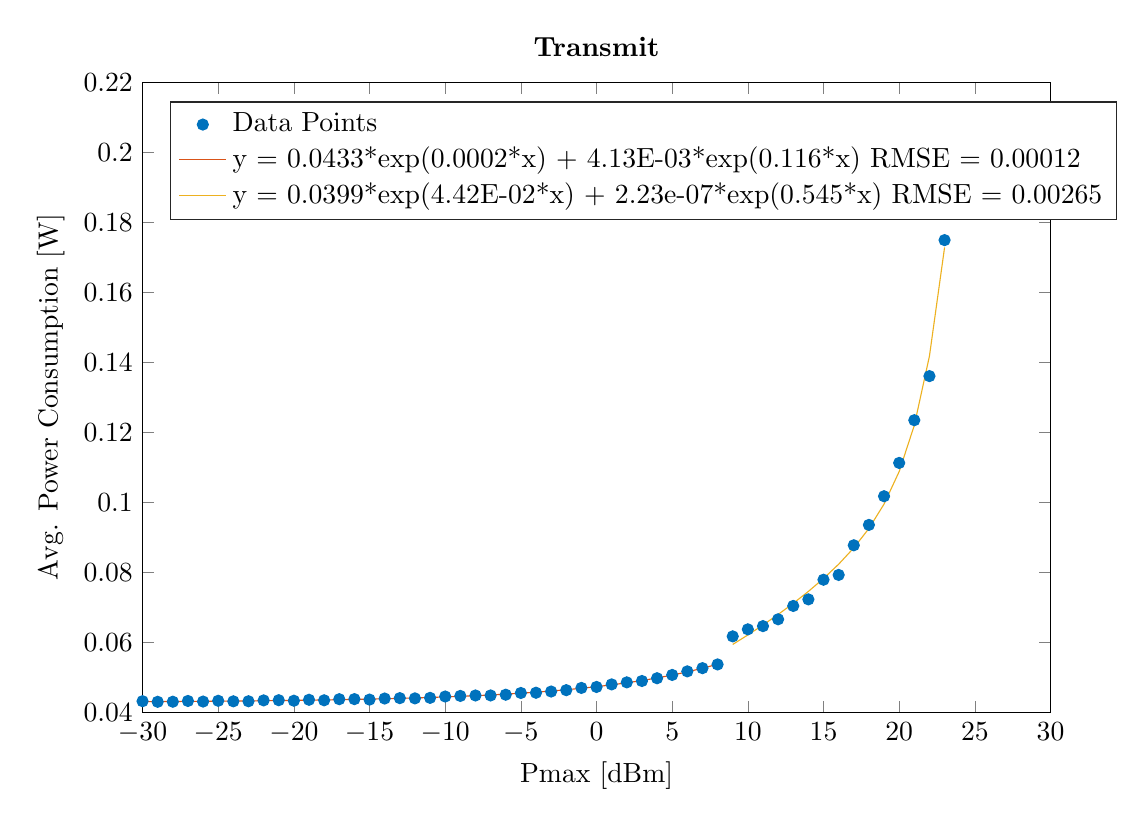
\begin{tikzpicture}

\begin{axis}[%
width=0.951\textwidth,
height=0.66\textwidth,
at={(0\textwidth,0\textwidth)},
scale only axis,
xmin=-30,
xmax=30,
xlabel={Pmax [dBm]},
ymin=0.04,
ymax=0.22,
ylabel={Avg. Power Consumption [W]},
axis background/.style={fill=white},
title style={font=\bfseries},
title={Transmit},
legend style={at={(0.03,0.97)},anchor=north west,legend cell align=left,align=left,draw=white!15!black},
y tick label style={/pgf/number format/fixed}
]
\addplot [color=mycolor1,only marks,mark=*,mark options={solid}]
  table[row sep=crcr]{%
10	0.0637950254237825\\
11	0.064713243745866\\
12	0.0666659683567463\\
13	0.0704764637679604\\
14	0.0723517382545409\\
15	0.077964939639652\\
16	0.079334950628774\\
17	0.0878082519401085\\
18	0.0936253392352084\\
19	0.101816405487039\\
20	0.111331959596792\\
21	0.123535456484453\\
22	0.136128742064438\\
23	0.174972950689174\\
9	0.0617877150990408\\
-1	0.0470602737490459\\
-10	0.0446109538683134\\
-11	0.0442200313078414\\
-12	0.0440716559725411\\
-13	0.0441436351842956\\
-14	0.0440310218032299\\
-15	0.0437250232069267\\
-16	0.043861312456332\\
-17	0.0438432049965383\\
-18	0.0435259843807757\\
-19	0.0436726853298729\\
-2	0.0464200132118457\\
-20	0.0434029278993332\\
-21	0.0435548718544184\\
-22	0.0434999814497639\\
-23	0.0432525264618958\\
-24	0.0432345150410041\\
-25	0.0433854386156806\\
-26	0.0431660444350098\\
-27	0.0433332959821664\\
-28	0.0431155547810735\\
-29	0.0430935271540902\\
-3	0.0460319501445317\\
-30	0.0432671370442985\\
-4	0.0456832887367053\\
-5	0.0456148403706944\\
-6	0.045118962743008\\
-7	0.0449127933362612\\
-8	0.0449036143685845\\
-9	0.0447768047382843\\
0	0.0473341788384111\\
1	0.0480683479919247\\
2	0.0486490752697266\\
3	0.0490368064453516\\
4	0.0498296655741014\\
5	0.0507689571429081\\
6	0.0517899366621504\\
7	0.0527056931949284\\
8	0.0537705239438872\\
};
\addlegendentry{Data Points};

\addplot [color=mycolor2,solid]
  table[row sep=crcr]{%
-30	0.0431292666676032\\
-29	0.0431542082548141\\
-28	0.0431810736294623\\
-27	0.0432100996121427\\
-26	0.0432415522070661\\
-25	0.0432757301983898\\
-24	0.0433129691897273\\
-23	0.0433536461414516\\
-22	0.0433981844671359\\
-21	0.0434470597580337\\
-20	0.0435008062129939\\
-19	0.043560023860741\\
-18	0.0436253866721654\\
-17	0.0436976516723004\\
-16	0.0437776691751785\\
-15	0.0438663942799402\\
-14	0.0439648997836222\\
-13	0.0440743906852025\\
-12	0.0441962204769953\\
-11	0.0443319094436535\\
-10	0.0444831652161776\\
-9	0.044651905858819\\
-8	0.0448402858010076\\
-7	0.0450507249649014\\
-6	0.045285941482356\\
-5	0.0455489884436444\\
-4	0.0458432951747622\\
-3	0.0461727136013829\\
-2	0.0465415703262953\\
-1	0.0469547251244026\\
0	0.0474176366461276\\
1	0.0479364362175212\\
2	0.0485180107348439\\
3	0.0491700957743394\\
4	0.0499013801760316\\
5	0.0507216235155014\\
6	0.0516417880518442\\
7	0.0526741869357233\\
8	0.05383265068127\\
};
\addlegendentry{y = 0.0433*exp(0.0002*x) + 4.13E-03*exp(0.116*x) RMSE = 0.00012};

\addplot [color=mycolor3,solid]
  table[row sep=crcr]
\caption{Average power consumption as a function of $P_{TX}$ during a transmit phase.}
\label{fig:Transmit_Pmax}
\end{figure}

The influence on the average power consumption can be modelled using two function which again can be contributed to the use of a power amplifier. This means that $P_{transmit}$ can be modelled as:

\begin{align}
&P_{transmit} \sim \text{Lognormal}(\mu_{Pmax},6.0040\cdot 10^{-6}) [W]\\ \nonumber
&\mu_{Pmax} = \begin{cases} 0.0433\cdot\exp{(0.0002\cdot x)} + 4.13\cdot10^{-3}\cdot\exp{(0.116\cdot x)} \quad for x \leq 8 dBm \\
0.0399\cdot\exp{(0.0442\cdot x)} + 22.3\cdot10^{-6}\cdot\exp{(0.545\cdot x)} \quad for x > 8 dBm \end{cases}
\end{align}


\section{Idle Mode Power Consumption}
The idle mode power consumption involves the elements $P_{eDRX}$ and $P_{PSM}$, to measure those the device is release from the cell after the desired idle mode is enabled. The procedure used to measure the idle modes can be found in \appref{app:test_procedures}. The raw data from each of the idle mode measurements can be seen in the following figures.

\begin{minipage}{0.48\textwidth}
\begin{figure}[H]
\tikzsetnextfilename{DRX1}
\centering
\resizebox{\textwidth}{!}{
% This file was created by matlab2tikz.
%
%The latest updates can be retrieved from
%  http://www.mathworks.com/matlabcentral/fileexchange/22022-matlab2tikz-matlab2tikz
%where you can also make suggestions and rate matlab2tikz.
%
\definecolor{mycolor1}{rgb}{0.00000,0.44700,0.74100}%
%
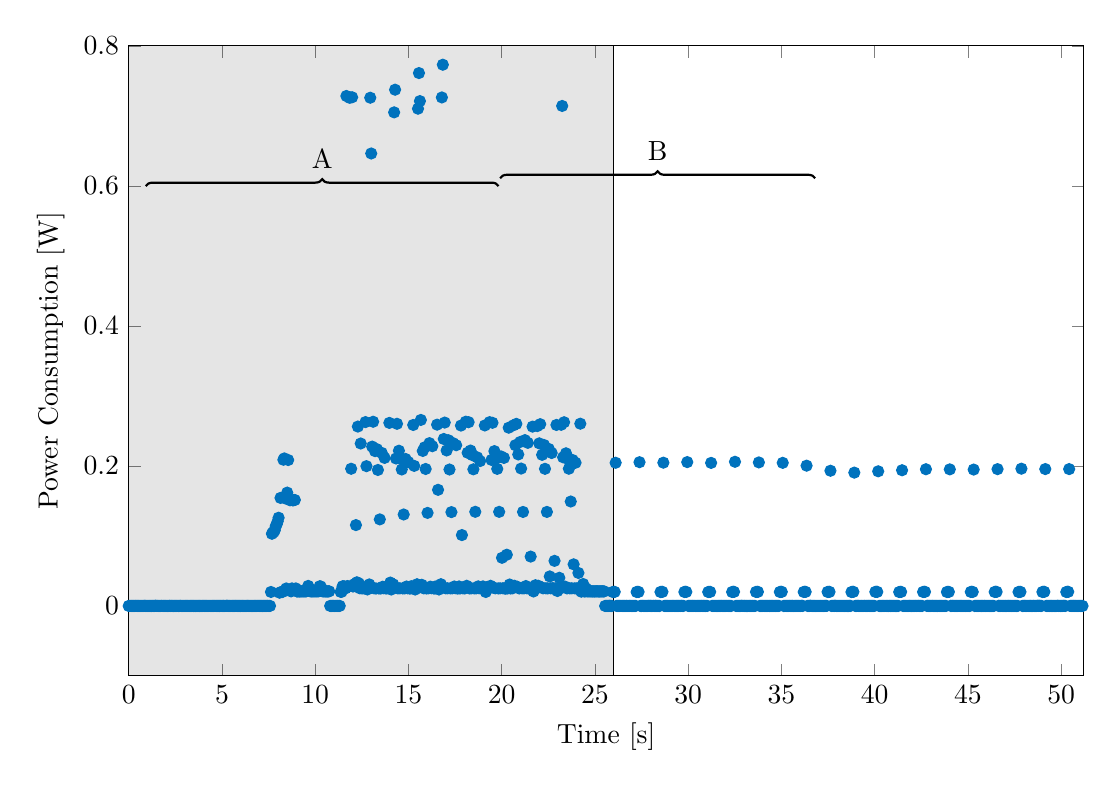
\begin{tikzpicture}

\begin{axis}[%
width=\textwidth,
height=0.66\textwidth,
at={(2.08in,0.858in)},
scale only axis,
xmin=0,
xmax=51.1998976,
xlabel={Time [s]},
ymin=-0.1,
ymax=0.8,
ylabel={Power Consumption [W]},
axis background/.style={fill=white},
%title style={font=\bfseries},
%title={$\text{DRXDefConfQuectel}_\text{\$}\text{1\$}$}
]
\addplot [color=mycolor1,only marks,mark=*,mark options={solid},forget plot]
  table[row sep=crcr]{%
0.0001024	-1.3347342e-05\\
0.0513024	3.01396464e-05\\
0.1025024	4.6453356e-05\\
0.1537024	1.9208808e-05\\
0.2049024	1.67797332e-05\\
0.2561024	-1.01010312e-05\\
0.3073024	-1.43632296e-05\\
0.3585024	4.8192588e-05\\
0.4097024	2.50241724e-05\\
0.4609024	-2.46168108e-05\\
0.5121024	9.6894792e-07\\
0.5633024	3.00072132e-06\\
0.6145024	-4.7064384e-06\\
0.6657024	4.583394e-05\\
0.7169024	1.4475546e-06\\
0.7681024	1.6579404e-06\\
0.8193024	3.7063944e-05\\
0.8705024	0.000157729824\\
0.9217024	-2.13939684e-05\\
0.9729024	4.1361336e-05\\
1.0241024	-1.28243124e-07\\
1.0753024	-3.00700764e-05\\
1.1265024	-1.65584484e-05\\
1.1777024	2.282895e-05\\
1.2289024	-3.5255124e-05\\
1.2801024	2.71732932e-05\\
1.3313024	1.39189896e-05\\
1.3825024	2.02255308e-05\\
1.4337024	0.000240173388\\
1.4849024	1.77495192e-05\\
1.5361024	5.4253548e-05\\
1.5873024	1.98978012e-05\\
1.6385024	-4.7446596e-05\\
1.6897024	3.25720764e-06\\
1.7409024	7.7375016e-05\\
1.7921024	3.53003868e-05\\
1.8433024	3.0104442e-05\\
1.8945024	2.18717388e-05\\
1.9457024	-7.578918e-06\\
1.9969024	-7.1237808e-06\\
2.0481024	8.8395552e-06\\
2.0993024	5.0090256e-06\\
2.1505024	-1.59046596e-05\\
2.2017024	6.464628e-05\\
2.2529024	-1.65006144e-05\\
2.3041024	5.2467372e-05\\
2.3553024	-1.1801718e-06\\
2.4065024	-4.3452612e-05\\
2.4577024	-2.37870036e-05\\
2.5089024	4.6469268e-06\\
2.5601024	-6.014016e-06\\
2.6113024	1.9419192e-05\\
2.6625024	-6.0011064e-05\\
2.7137024	-7.1698788e-06\\
2.7649024	8.1789768e-05\\
2.8161024	-4.5204444e-05\\
2.8673024	1.88006076e-05\\
2.9185024	2.73836772e-05\\
2.9697024	1.80177408e-05\\
3.0209024	-6.8547204e-06\\
3.0721024	-6.7960476e-06\\
3.1233024	2.99175264e-05\\
3.1745024	1.13382e-05\\
3.2257024	2.52462924e-05\\
3.2769024	1.57755816e-05\\
3.3281024	3.09459852e-06\\
3.3793024	6.5504556e-06\\
3.4305024	4.1524776e-05\\
3.4817024	-3.9143484e-05\\
3.5329024	-1.06617816e-05\\
3.5841024	-6.2428428e-05\\
3.6353024	-2.18725776e-05\\
3.6865024	2.73132684e-05\\
3.7377024	-1.86606324e-05\\
3.7889024	-1.3803318e-05\\
3.8401024	2.94389208e-05\\
3.8913024	-3.01748508e-05\\
3.9425024	4.4256456e-06\\
3.9937024	3.86523e-05\\
4.0449024	3.50279748e-06\\
4.0961024	4.1770368e-05\\
4.1473024	2.7827082e-05\\
4.1985024	-5.78016e-06\\
4.2497024	-4.618512e-05\\
4.3009024	3.13659216e-05\\
4.3521024	3.322251e-05\\
4.4033024	2.58766128e-05\\
4.4545024	-8.1396648e-06\\
4.5057024	1.68618744e-05\\
4.5569024	2.7079416e-05\\
4.6081024	1.4444532e-05\\
4.6593024	3.58728696e-05\\
4.7105024	8.453988e-06\\
4.7617024	1.95709068e-05\\
4.8129024	1.88467092e-05\\
4.8641024	-3.06182556e-05\\
4.9153024	1.43858592e-05\\
4.9665024	4.0042044e-05\\
5.0177024	2.6503578e-06\\
5.0689024	4.8905064e-05\\
5.1201024	-1.8625428e-05\\
5.1713024	1.83328992e-05\\
5.2225024	2.27585448e-05\\
5.2737024	0.000242287308\\
5.3249024	-1.41880464e-05\\
5.3761024	3.21479532e-05\\
5.4273024	6.083586e-06\\
5.4785024	3.28947804e-05\\
5.5297024	2.82822192e-05\\
5.5809024	6.7021704e-06\\
5.6321024	1.56238668e-05\\
5.6833024	-6.6795372e-06\\
5.7345024	6.2427564e-05\\
5.7857024	3.7904652e-05\\
5.8369024	5.7332232e-06\\
5.8881024	4.1945544e-05\\
5.9393024	-3.14824284e-05\\
5.9905024	-4.952448e-05\\
6.0417024	3.9646404e-07\\
6.0929024	1.36625004e-05\\
6.1441024	3.08278008e-05\\
6.1953024	-3.9505572e-05\\
6.2465024	-2.19890844e-05\\
6.2977024	-3.9587724e-06\\
6.3489024	5.941512e-05\\
6.4001024	6.076962e-05\\
6.4513024	-4.0964868e-05\\
6.5025024	-2.33553348e-05\\
6.5537024	1.13239512e-06\\
6.6049024	-1.11403872e-05\\
6.6561024	-7.4733048e-06\\
6.7073024	-2.5153254e-05\\
6.7585024	1.12568976e-05\\
6.8097024	5.0676984e-06\\
6.8609024	-1.36516068e-05\\
6.9121024	2.32614576e-05\\
6.9633024	4.5215352e-05\\
7.0145024	-1.47186216e-06\\
7.0657024	2.66242788e-05\\
7.1169024	7.9376616e-07\\
7.1681024	-3.9003516e-05\\
7.2193024	-8.9334324e-06\\
7.2705024	1.86480576e-05\\
7.3217024	1.08947988e-05\\
7.3729024	1.83681036e-05\\
7.4241024	5.1567984e-05\\
7.4753024	1.8403308e-05\\
7.5265024	-1.5122628e-05\\
7.5777024	4.3837344e-05\\
7.6289024	0.0199351152\\
7.6801024	0.10303776\\
7.7313024	0.104827716\\
7.7825024	0.105791364\\
7.8337024	0.108096444\\
7.8849024	0.11392794\\
7.9361024	0.116557272\\
7.9873024	0.120682872\\
8.0385024	0.12594384\\
8.0897024	0.0188719452\\
8.1409024	0.154284408\\
8.1921024	0.0200538612\\
8.2433024	0.0199176012\\
8.2945024	0.208794564\\
8.3457024	0.210701088\\
8.3969024	0.15352128\\
8.4481024	0.0249259752\\
8.4993024	0.161845524\\
8.5505024	0.208368252\\
8.6017024	0.0228432528\\
8.6529024	0.150860304\\
8.7041024	0.0207715572\\
8.7553024	0.0250076124\\
8.8065024	0.150689268\\
8.8577024	0.15134994\\
8.9089024	0.1512909\\
8.9601024	0.0250060788\\
9.0113024	0.020781072\\
9.0625024	0.0207200124\\
9.1137024	0.0208070388\\
9.1649024	0.0206997696\\
9.2161024	0.0207937476\\
9.2673024	0.0207832428\\
9.3185024	0.0208215396\\
9.3697024	0.0208099908\\
9.4209024	0.0207891864\\
9.4721024	0.0208092132\\
9.5233024	0.0208234476\\
9.5745024	0.0249726024\\
9.6257024	0.0285985944\\
9.6769024	0.0250067628\\
9.7281024	0.0209289132\\
9.7793024	0.0208719684\\
9.8305024	0.0207531648\\
9.8817024	0.0208653804\\
9.9329024	0.02086911\\
9.9841024	0.020876166\\
10.0353024	0.0208785312\\
10.0865024	0.020900088\\
10.1377024	0.0208500444\\
10.1889024	0.0208981584\\
10.2401024	0.0280131732\\
10.2913024	0.0278755236\\
10.3425024	0.0250580016\\
10.3937024	0.0208112724\\
10.4449024	0.0208738296\\
10.4961024	0.0207869292\\
10.5473024	0.0207606888\\
10.5985024	0.0207415188\\
10.6497024	0.0207309708\\
10.7009024	0.020779308\\
10.7521024	0.0208486584\\
10.8033024	1.1572056e-05\\
10.8545024	-1.51804656e-05\\
10.9057024	-1.28494584e-06\\
10.9569024	1.21906404e-05\\
11.0081024	-1.94200308e-05\\
11.0593024	-5.3612316e-05\\
11.1105024	4.3669728e-06\\
11.1617024	2.75471244e-05\\
11.2129024	2.11240728e-05\\
11.2641024	-1.04865984e-05\\
11.3153024	4.2774516e-05\\
11.3665024	0.0200678292\\
11.4177024	0.020173842\\
11.4689024	0.0280076076\\
11.5201024	0.0279150768\\
11.5713024	0.0277283556\\
11.6225024	0.0249987024\\
11.6737024	0.728325\\
11.7249024	0.0283334976\\
11.7761024	0.02777445\\
11.8273024	0.72592164\\
11.8785024	0.72608184\\
11.9297024	0.195912792\\
11.9809024	0.72651672\\
12.0321024	0.027727182\\
12.0833024	0.0308310624\\
12.1345024	0.030968568\\
12.1857024	0.115462332\\
12.2369024	0.0337531356\\
12.2881024	0.256169808\\
12.3393024	0.0323021664\\
12.3905024	0.0251955972\\
12.4417024	0.23196726\\
12.4929024	0.0251941572\\
12.5441024	0.0250945812\\
12.5953024	0.0267261228\\
12.6465024	0.0250068456\\
12.6977024	0.26257392\\
12.7489024	0.199599768\\
12.8001024	0.0235381464\\
12.8513024	0.0277234164\\
12.9025024	0.0307102464\\
12.9537024	0.72585288\\
13.0049024	0.64620216\\
13.0561024	0.227542824\\
13.1073024	0.263043684\\
13.1585024	0.0251079408\\
13.2097024	0.221081652\\
13.2609024	0.024917364\\
13.3121024	0.223861932\\
13.3633024	0.19419228\\
13.4145024	0.0249408324\\
13.4657024	0.123592716\\
13.5169024	0.0248616828\\
13.5681024	0.218612412\\
13.6193024	0.0273884112\\
13.6705024	0.0252271692\\
13.7217024	0.211425156\\
13.7729024	0.025119558\\
13.8241024	0.0250067052\\
13.8753024	0.028041642\\
13.9265024	0.0251603676\\
13.9777024	0.261418536\\
14.0289024	0.0333495684\\
14.0801024	0.0234402552\\
14.1313024	0.0277242516\\
14.1825024	0.030903066\\
14.2337024	0.70493328\\
14.2849024	0.73729692\\
14.3361024	0.210575484\\
14.3873024	0.260115408\\
14.4385024	0.025053948\\
14.4897024	0.221661252\\
14.5409024	0.0251830152\\
14.5921024	0.209955564\\
14.6433024	0.194872572\\
14.6945024	0.0250024932\\
14.7457024	0.1305837\\
14.7969024	0.0250194384\\
14.8481024	0.209866716\\
14.8993024	0.027714348\\
14.9505024	0.0252617112\\
15.0017024	0.205328844\\
15.0529024	0.0249093108\\
15.1041024	0.0250121376\\
15.1553024	0.0281312136\\
15.2065024	0.0252221832\\
15.2577024	0.258469128\\
15.3089024	0.200008476\\
15.3601024	0.0234274932\\
15.4113024	0.027740934\\
15.4625024	0.0309356928\\
15.5137024	0.71017452\\
15.5649024	0.7610778\\
15.6161024	0.72104652\\
15.6673024	0.265644036\\
15.7185024	0.0301432572\\
15.7697024	0.221364036\\
15.8209024	0.02509056\\
15.8721024	0.226569636\\
15.9233024	0.195592968\\
15.9745024	0.0249082308\\
16.0257024	0.132866352\\
16.0769024	0.025156962\\
16.1281024	0.232486308\\
16.1793024	0.0275248116\\
16.2305024	0.0252820548\\
16.2817024	0.22811634\\
16.3329024	0.0253370376\\
16.3841024	0.0247916412\\
16.4353024	0.0276118776\\
16.4865024	0.025149042\\
16.5377024	0.25890354\\
16.5889024	0.165810636\\
16.6401024	0.0234741924\\
16.6913024	0.0277516008\\
16.7425024	0.0310229784\\
16.7937024	0.72624204\\
16.8449024	0.77297976\\
16.8961024	0.238438764\\
16.9473024	0.261871272\\
16.9985024	0.025118478\\
17.0497024	0.22203954\\
17.1009024	0.0251678052\\
17.1521024	0.23655438\\
17.2033024	0.194836068\\
17.2545024	0.0250567812\\
17.3057024	0.1339794\\
17.3569024	0.02519109\\
17.4081024	0.232363188\\
17.4593024	0.0277310196\\
17.5105024	0.0252927684\\
17.5617024	0.229553172\\
17.6129024	0.0249882984\\
17.6641024	0.025060068\\
17.7153024	0.0278109252\\
17.7665024	0.0249430284\\
17.8177024	0.2575989\\
17.8689024	0.101195028\\
17.9201024	0.0250827948\\
17.9713024	0.0266997312\\
18.0225024	0.024985404\\
18.0737024	0.263091384\\
18.1249024	0.0287482788\\
18.1761024	0.218758788\\
18.2273024	0.262426104\\
18.2785024	0.0249756192\\
18.3297024	0.221911812\\
18.3809024	0.0251394408\\
18.4321024	0.215327412\\
18.4833024	0.195097248\\
18.5345024	0.0250595244\\
18.5857024	0.134426412\\
18.6369024	0.0250777764\\
18.6881024	0.212219028\\
18.7393024	0.027910782\\
18.7905024	0.0252245268\\
18.8417024	0.20687868\\
18.8929024	0.0251775648\\
18.9441024	0.0250093512\\
18.9953024	0.0278805384\\
19.0465024	0.0253429992\\
19.0977024	0.257762016\\
19.1489024	0.019898802\\
19.2001024	0.0252754164\\
19.2513024	0.0270424908\\
19.3025024	0.0250199856\\
19.3537024	0.262497168\\
19.4049024	0.0287253792\\
19.4561024	0.208518336\\
19.5073024	0.261546156\\
19.5585024	0.0260910396\\
19.6097024	0.22109094\\
19.6609024	0.0250980156\\
19.7121024	0.210750552\\
19.7633024	0.195751764\\
19.8145024	0.0250226892\\
19.8657024	0.134345196\\
19.9169024	0.025092324\\
19.9681024	0.213509628\\
20.0193024	0.068726484\\
20.0705024	0.0252628632\\
20.1217024	0.211375152\\
20.1729024	0.024901092\\
20.2241024	0.0247144788\\
20.2753024	0.073123992\\
20.3265024	0.0250517376\\
20.3777024	0.254542428\\
20.4289024	0.0305754012\\
20.4801024	0.0249196608\\
20.5313024	0.028073034\\
20.5825024	0.0251284248\\
20.6337024	0.25800012\\
20.6849024	0.0287396352\\
20.7361024	0.229525344\\
20.7873024	0.260032824\\
20.8385024	0.0273174084\\
20.8897024	0.216350748\\
20.9409024	0.0249624864\\
20.9921024	0.234159912\\
21.0433024	0.196200216\\
21.0945024	0.0251046612\\
21.1457024	0.134225856\\
21.1969024	0.025105824\\
21.2481024	0.23679306\\
21.2993024	0.0283907592\\
21.3505024	0.0252085068\\
21.4017024	0.232931232\\
21.4529024	0.0249138072\\
21.5041024	0.02512287\\
21.5553024	0.070455564\\
21.6065024	0.0251048952\\
21.6577024	0.256064328\\
21.7089024	0.0206443476\\
21.7601024	0.024905034\\
21.8113024	0.0295501572\\
21.8625024	0.0250314624\\
21.9137024	0.256896684\\
21.9649024	0.0287357652\\
22.0161024	0.232188336\\
22.0673024	0.259568244\\
22.1185024	0.0267835212\\
22.1697024	0.215772732\\
22.2209024	0.0251327448\\
22.2721024	0.229847832\\
22.3233024	0.195798312\\
22.3745024	0.0251154108\\
22.4257024	0.13424472\\
22.4769024	0.0250659828\\
22.5281024	0.22423158\\
22.5793024	0.042133032\\
22.6305024	0.0251454132\\
22.6817024	0.218408868\\
22.7329024	0.02526516\\
22.7841024	0.0249169968\\
22.8353024	0.064354752\\
22.8865024	0.0251093556\\
22.9377024	0.258482052\\
22.9889024	0.0213241032\\
23.0401024	0.024943518\\
23.0913024	0.04018518\\
23.1425024	0.0249809508\\
23.1937024	0.258717096\\
23.2449024	0.71411148\\
23.2961024	0.212285412\\
23.3473024	0.262335636\\
23.3985024	0.027599922\\
23.4497024	0.217956348\\
23.5009024	0.0250252092\\
23.5521024	0.209873052\\
23.6033024	0.195941016\\
23.6545024	0.0250895124\\
23.7057024	0.149109876\\
23.7569024	0.0251678268\\
23.8081024	0.2083446\\
23.8593024	0.05939748\\
23.9105024	0.0250814232\\
23.9617024	0.20447964\\
24.0129024	0.0249591924\\
24.0641024	0.024959934\\
24.1153024	0.047088432\\
24.1665024	0.025109046\\
24.2177024	0.260258004\\
24.2689024	0.0203570316\\
24.3201024	0.023549958\\
24.3713024	0.0312678288\\
24.4225024	0.0207306864\\
24.4737024	0.0206958492\\
24.5249024	0.0250086636\\
24.5761024	0.0208189224\\
24.6273024	0.0208302624\\
24.6785024	0.0208787832\\
24.7297024	0.0208354248\\
24.7809024	0.0208027152\\
24.8321024	0.020807352\\
24.8833024	0.020761992\\
24.9345024	0.020790828\\
24.9857024	0.020681604\\
25.0369024	0.020803932\\
25.0881024	0.0208750104\\
25.1393024	0.020802978\\
25.1905024	0.0207509148\\
25.2417024	0.0206656164\\
25.2929024	0.0207867384\\
25.3441024	0.0207752328\\
25.3953024	0.020853792\\
25.4465024	0.0207490644\\
25.4977024	0.0207474192\\
25.5489024	-5.7173796e-05\\
25.6001024	4.9640976e-05\\
25.6513024	1.4690124e-05\\
25.7025024	-5.6167128e-06\\
25.7537024	4.876506e-05\\
25.8049024	0.0001505943\\
25.8561024	-4.9402944e-06\\
25.9073024	-5.877306e-05\\
25.9585024	0.019907352\\
26.0097024	0.0200097144\\
26.0609024	0.0200609928\\
26.1121024	0.204453504\\
26.1633024	4.2552396e-05\\
26.2145024	1.31361192e-05\\
26.2657024	-1.89179568e-06\\
26.3169024	2.05172208e-05\\
26.3681024	2.56083912e-05\\
26.4193024	3.44596788e-05\\
26.4705024	1.69666488e-05\\
26.5217024	4.2097284e-05\\
26.5729024	4.4187732e-05\\
26.6241024	-3.8746188e-05\\
26.6753024	5.1158952e-05\\
26.7265024	6.3518076e-06\\
26.7777024	-1.32073632e-05\\
26.8289024	-1.72474416e-05\\
26.8801024	5.8247532e-05\\
26.9313024	1.9710882e-05\\
26.9825024	-4.6008252e-06\\
27.0337024	4.6703952e-06\\
27.0849024	-3.845448e-05\\
27.1361024	3.07347624e-05\\
27.1873024	3.50556336e-05\\
27.2385024	0.0199123812\\
27.2897024	0.0200673504\\
27.3409024	0.0200144844\\
27.3921024	0.205295724\\
27.4433024	-7.124616e-07\\
27.4945024	-3.9248244e-05\\
27.5457024	7.694334e-05\\
27.5969024	-8.594802e-06\\
27.6481024	-1.3125222e-05\\
27.6993024	-2.22338376e-05\\
27.7505024	-2.54223108e-05\\
27.8017024	3.7944864e-06\\
27.8529024	6.5160072e-05\\
27.9041024	8.640234e-05\\
27.9553024	4.8846384e-05\\
28.0065024	4.8788532e-05\\
28.0577024	-3.8653164e-05\\
28.1089024	4.2035256e-06\\
28.1601024	7.00065e-05\\
28.2113024	-2.83811256e-06\\
28.2625024	5.530464e-05\\
28.3137024	-3.5009532e-05\\
28.3649024	-1.4601276e-06\\
28.4161024	3.701448e-06\\
28.4673024	-4.3557408e-05\\
28.5185024	0.0198970236\\
28.5697024	0.019943568\\
28.6209024	0.0200915424\\
28.6721024	0.204602292\\
28.7233024	-3.3628194e-06\\
28.7745024	4.53042e-06\\
28.8257024	-4.6477656e-06\\
28.8769024	2.87264592e-05\\
28.9281024	9.2368584e-06\\
28.9793024	3.25100484e-05\\
29.0305024	-3.42149292e-06\\
29.0817024	-4.2950556e-05\\
29.1329024	-1.21680072e-05\\
29.1841024	6.8255496e-05\\
29.2353024	1.47831624e-05\\
29.2865024	1.67101632e-05\\
29.3377024	4.4139096e-06\\
29.3889024	3.9061332e-05\\
29.4401024	3.06760896e-05\\
29.4913024	1.09878372e-05\\
29.5425024	2.9088558e-05\\
29.5937024	-9.5721336e-07\\
29.6449024	9.5137128e-05\\
29.6961024	-3.48016608e-06\\
29.7473024	1.40589648e-05\\
29.7985024	0.019943406\\
29.8497024	0.0201050676\\
29.9009024	0.0200327472\\
29.9521024	0.205416684\\
30.0033024	3.22409916e-05\\
30.0545024	-6.4808892e-06\\
30.1057024	5.5456344e-05\\
30.1569024	-1.48535712e-05\\
30.2081024	8.208396e-06\\
30.2593024	5.7710232e-05\\
30.3105024	4.5530496e-05\\
30.3617024	-4.0291812e-06\\
30.4129024	-1.48653036e-05\\
30.4641024	-1.63715328e-05\\
30.5153024	-5.3132868e-06\\
30.5665024	2.81891772e-05\\
30.6177024	1.55886624e-05\\
30.6689024	2.4475158e-07\\
30.7201024	5.6869524e-05\\
30.7713024	4.3171848e-05\\
30.8225024	5.7044736e-05\\
30.8737024	1.18176444e-05\\
30.9249024	-1.85793264e-05\\
30.9761024	3.34789992e-05\\
31.0273024	1.78542936e-05\\
31.0785024	0.0198766872\\
31.1297024	0.0199951524\\
31.1809024	0.0200548008\\
31.2321024	0.204279588\\
31.2833024	4.7048472e-05\\
31.3345024	2.57835708e-05\\
31.3857024	-4.6862388e-05\\
31.4369024	-5.3602272e-06\\
31.4881024	5.768424e-06\\
31.5393024	-3.662136e-05\\
31.5905024	5.6401812e-06\\
31.6417024	8.5243968e-06\\
31.6929024	2.90994516e-05\\
31.7441024	2.16144144e-05\\
31.7953024	5.4101844e-05\\
31.8465024	4.1683212e-06\\
31.8977024	-2.87381916e-05\\
31.9489024	1.28243124e-07\\
32.0001024	-1.86916428e-07\\
32.0513024	1.16650944e-05\\
32.1025024	4.6604232e-05\\
32.1537024	-1.39785012e-05\\
32.2049024	3.47404752e-05\\
32.2561024	-2.29580316e-05\\
32.3073024	-3.49391268e-05\\
32.3585024	0.0198829548\\
32.4097024	0.0201045204\\
32.4609024	0.0200977956\\
32.5121024	0.205858332\\
32.5633024	1.82515932e-05\\
32.6145024	7.0525332e-06\\
32.6657024	2.45572992e-05\\
32.7169024	-5.7360708e-05\\
32.7681024	7.7649948e-06\\
32.8193024	-1.45853496e-05\\
32.8705024	0.000196533828\\
32.9217024	1.68140988e-06\\
32.9729024	3.23231328e-05\\
33.0241024	4.898718e-05\\
33.0753024	-2.84900904e-06\\
33.1265024	-7.2448128e-05\\
33.1777024	-2.43594864e-05\\
33.2289024	1.2821796e-05\\
33.2801024	-5.3836956e-06\\
33.3313024	3.28134744e-05\\
33.3825024	-4.3669728e-06\\
33.4337024	3.255615e-05\\
33.4849024	-5.1813576e-05\\
33.5361024	2.92050648e-05\\
33.5873024	2.02716324e-05\\
33.6385024	0.0199823544\\
33.6897024	0.0200268\\
33.7409024	0.0200947392\\
33.7921024	0.20495286\\
33.8433024	-4.4958852e-05\\
33.8945024	1.04974956e-05\\
33.9457024	3.9785544e-05\\
33.9969024	1.48183668e-05\\
34.0481024	2.22103656e-05\\
34.0993024	1.46197152e-05\\
34.1505024	6.4574172e-06\\
34.2017024	3.6573588e-05\\
34.2529024	5.2655112e-06\\
34.3041024	2.75705928e-05\\
34.3553024	-5.1953544e-05\\
34.4065024	3.12720408e-05\\
34.4577024	-5.2319844e-06\\
34.5089024	4.0228956e-05\\
34.5601024	2.17552284e-05\\
34.6113024	3.12955128e-05\\
34.6625024	-3.6539244e-05\\
34.7137024	2.18834712e-05\\
34.7649024	1.22141088e-05\\
34.8161024	2.83760964e-05\\
34.8673024	4.6698084e-05\\
34.9185024	0.0199321344\\
34.9697024	0.0200574648\\
35.0209024	0.0200899728\\
35.0721024	0.204345576\\
35.1233024	-4.1023548e-05\\
35.1745024	1.48275864e-06\\
35.2257024	2.56318596e-05\\
35.2769024	-8.5478652e-06\\
35.3281024	1.04740272e-05\\
35.3793024	-6.29397e-06\\
35.4305024	6.1120008e-05\\
35.4817024	3.759282e-06\\
35.5329024	-1.02527424e-05\\
35.5841024	4.8613356e-05\\
35.6353024	-1.79951076e-05\\
35.6865024	-6.0093216e-05\\
35.7377024	-4.2856668e-06\\
35.7889024	5.3716248e-05\\
35.8401024	-1.3650768e-05\\
35.8913024	1.95826392e-05\\
35.9425024	-3.31060032e-05\\
35.9937024	1.61728812e-05\\
36.0449024	-2.338551e-07\\
36.0961024	0.000175899276\\
36.1473024	2.26655028e-05\\
36.1985024	0.0199526328\\
36.2497024	0.0200850336\\
36.3009024	0.0200841192\\
36.3521024	0.200312352\\
36.4033024	2.22916716e-05\\
36.4545024	1.45727784e-05\\
36.5057024	-2.98948968e-05\\
36.5569024	0.0002582037\\
36.6081024	3.39576048e-05\\
36.6593024	-4.5195228e-06\\
36.7105024	8.967798e-06\\
36.7617024	8.523558e-06\\
36.8129024	-1.74930336e-05\\
36.8641024	-1.98164952e-05\\
36.9153024	1.72591776e-05\\
36.9665024	-5.2437204e-06\\
37.0177024	-2.88907452e-05\\
37.0689024	2.82126492e-05\\
37.1201024	1.8694998e-05\\
37.1713024	1.12099572e-05\\
37.2225024	-3.7169532e-05\\
37.2737024	-4.4030124e-06\\
37.3249024	1.89179568e-06\\
37.3761024	4.9127184e-05\\
37.4273024	5.038866e-05\\
37.4785024	0.0199912572\\
37.5297024	0.0199704384\\
37.5809024	0.0200724624\\
37.6321024	0.19306944\\
37.6833024	-6.4691532e-06\\
37.7345024	8.5126608e-06\\
37.7857024	4.063716e-05\\
37.8369024	4.7340144e-05\\
37.8881024	0.000190987524\\
37.9393024	-3.8466216e-05\\
37.9905024	-5.6484792e-05\\
38.0417024	4.3743492e-05\\
38.0929024	1.26231444e-05\\
38.1441024	-2.61582444e-05\\
38.1953024	-1.4620554e-05\\
38.2465024	-7.122942e-06\\
38.2977024	3.7333008e-05\\
38.3489024	-5.05521e-05\\
38.4001024	1.10892564e-06\\
38.4513024	-3.6866124e-05\\
38.5025024	4.5647856e-06\\
38.5537024	-5.2327368e-05\\
38.6049024	-4.6652004e-05\\
38.6561024	6.7098816e-05\\
38.7073024	5.5515024e-05\\
38.7585024	0.0198180468\\
38.8097024	0.0200715696\\
38.8609024	0.0201181536\\
38.9121024	0.190391148\\
38.9633024	-1.42701912e-05\\
39.0145024	-2.1256506e-06\\
39.0657024	7.4421252e-05\\
39.1169024	6.3222192e-05\\
39.1681024	-8.1975024e-06\\
39.2193024	-6.3526428e-06\\
39.2705024	-2.3822208e-05\\
39.3217024	-2.84900904e-06\\
39.3729024	2.20469184e-05\\
39.4241024	3.37455432e-06\\
39.4753024	6.3245664e-05\\
39.5265024	1.22543424e-06\\
39.5777024	6.7139028e-06\\
39.6289024	-1.40363352e-05\\
39.6801024	5.902956e-05\\
39.7313024	-2.09044656e-06\\
39.7825024	2.9905794e-05\\
39.8337024	-1.7518176e-07\\
39.8849024	-4.2395652e-06\\
39.9361024	-2.97901224e-05\\
39.9873024	2.14861716e-05\\
40.0385024	0.0200774052\\
40.0897024	0.0200886048\\
40.1409024	0.0200652048\\
40.1921024	0.192271428\\
40.2433024	1.36742364e-05\\
40.2945024	-1.44688428e-05\\
40.3457024	-5.2584696e-05\\
40.3969024	-3.12980256e-06\\
40.4481024	3.1213368e-05\\
40.4993024	-7.1816148e-06\\
40.5505024	3.7029564e-05\\
40.6017024	2.35648836e-05\\
40.6529024	2.15557416e-05\\
40.7041024	1.23188832e-05\\
40.7553024	-5.6986884e-05\\
40.8065024	5.32494e-05\\
40.8577024	-5.8154472e-05\\
40.9089024	8.1723564e-07\\
40.9601024	1.54604196e-05\\
41.0113024	-2.75353884e-05\\
41.0625024	1.47102408e-06\\
41.1137024	-2.75353884e-05\\
41.1649024	-1.98282312e-05\\
41.2161024	1.8391572e-05\\
41.2673024	5.6988576e-06\\
41.3185024	0.0198292284\\
41.3697024	0.0200469168\\
41.4209024	0.0200438604\\
41.4721024	0.193774392\\
41.5233024	-2.583135e-05\\
41.5745024	3.40749504e-05\\
41.6257024	3.02326848e-05\\
41.6769024	-3.00072132e-06\\
41.7281024	2.39269824e-05\\
41.7793024	-5.71059e-06\\
41.8305024	7.9376616e-07\\
41.8817024	6.0933096e-05\\
41.9329024	1.60555356e-05\\
41.9841024	-3.6690948e-05\\
42.0353024	1.11630204e-05\\
42.0865024	-2.27476476e-05\\
42.1377024	-1.21445388e-05\\
42.1889024	4.8309948e-05\\
42.2401024	1.04773788e-07\\
42.2913024	1.54721556e-05\\
42.3425024	5.9999328e-05\\
42.3937024	3.3023862e-05\\
42.4449024	3.7566e-05\\
42.4961024	2.79905292e-05\\
42.5473024	-1.10699784e-05\\
42.5985024	0.0199399572\\
42.6497024	0.0200525976\\
42.7009024	0.0201307608\\
42.7521024	0.19522116\\
42.8033024	5.963724e-05\\
42.8545024	6.8149908e-05\\
42.9057024	2.048202e-05\\
42.9569024	1.34521164e-05\\
43.0081024	8.0105832e-06\\
43.0593024	3.47404752e-05\\
43.1105024	5.049342e-05\\
43.1617024	-2.28063204e-05\\
43.2129024	2.3810472e-05\\
43.2641024	3.53800116e-06\\
43.3153024	-3.6960012e-05\\
43.3665024	-1.89992592e-05\\
43.4177024	3.26382912e-05\\
43.4689024	-2.96845092e-05\\
43.5201024	-3.50363556e-06\\
43.5713024	1.16064216e-05\\
43.6225024	1.6324596e-05\\
43.6737024	4.6522908e-05\\
43.7249024	-5.0541192e-05\\
43.7761024	6.3969012e-05\\
43.8273024	7.1698788e-06\\
43.8785024	0.0198715788\\
43.9297024	0.0200436624\\
43.9809024	0.020019798\\
44.0321024	0.195036732\\
44.0833024	5.6857788e-05\\
44.1345024	1.83563676e-05\\
44.1857024	5.3050752e-05\\
44.2369024	8.687844e-06\\
44.2881024	1.03851792e-06\\
44.3393024	-7.8940764e-06\\
44.3905024	-3.8255832e-05\\
44.4417024	-3.10633344e-06\\
44.4929024	3.7262592e-05\\
44.5441024	1.54025856e-05\\
44.5953024	1.58753232e-06\\
44.6465024	1.03809888e-05\\
44.6977024	-7.2419652e-07\\
44.7489024	1.0076724e-05\\
44.8001024	1.25292672e-05\\
44.8513024	-3.26039256e-05\\
44.9025024	7.6828536e-06\\
44.9537024	-2.34483732e-05\\
45.0049024	3.6970884e-05\\
45.0561024	1.09526328e-05\\
45.1073024	-8.396154e-06\\
45.1585024	0.0200032056\\
45.2097024	0.020094462\\
45.2609024	0.0199887588\\
45.3121024	0.194746716\\
45.3633024	-8.1161964e-06\\
45.4145024	2.33310276e-05\\
45.4657024	1.79129664e-05\\
45.5169024	2.05172208e-05\\
45.5681024	-8.0692596e-06\\
45.6193024	2.82822192e-05\\
45.6705024	-3.22284168e-06\\
45.7217024	-5.2969428e-05\\
45.7729024	2.98898676e-06\\
45.8241024	-2.13470316e-05\\
45.8753024	6.9492672e-05\\
45.9265024	-3.23239716e-05\\
45.9777024	-1.43749656e-05\\
46.0289024	-2.27736324e-06\\
46.0801024	-2.04476544e-05\\
46.1313024	8.3374776e-06\\
46.1825024	-4.5122292e-05\\
46.2337024	-2.97892836e-05\\
46.2849024	3.8472948e-07\\
46.3361024	2.18834712e-05\\
46.3873024	-4.3078788e-05\\
46.4385024	0.0199598508\\
46.4897024	0.0201514572\\
46.5409024	0.020082114\\
46.5921024	0.195359076\\
46.6433024	5.0889888e-05\\
46.6945024	3.6001116e-05\\
46.7457024	1.05327e-05\\
46.7969024	2.4931134e-05\\
46.8481024	-2.16085464e-06\\
46.8993024	-2.11391604e-06\\
46.9505024	-2.8190016e-05\\
47.0017024	2.53167012e-05\\
47.0529024	-2.30980104e-05\\
47.1041024	1.10113056e-05\\
47.1553024	6.221718e-05\\
47.2065024	-8.1975024e-06\\
47.2577024	4.4408988e-05\\
47.3089024	1.09643688e-05\\
47.3601024	1.16759916e-06\\
47.4113024	-8.1396648e-06\\
47.4625024	-3.58032996e-05\\
47.5137024	3.58611336e-05\\
47.5649024	-8.0223192e-06\\
47.6161024	-2.22807744e-05\\
47.6673024	1.30204476e-05\\
47.7185024	0.0198962604\\
47.7697024	0.0200421864\\
47.8209024	0.0200440332\\
47.8721024	0.196013052\\
47.9233024	-1.9817334e-05\\
47.9745024	2.64608316e-05\\
48.0257024	6.6153348e-05\\
48.0769024	2.43586476e-05\\
48.1281024	-2.68639992e-06\\
48.1793024	3.03726636e-05\\
48.2305024	1.55895012e-05\\
48.2817024	1.76330088e-05\\
48.3329024	5.1649272e-05\\
48.3841024	-1.96999884e-05\\
48.4353024	-2.85169104e-05\\
48.4865024	-3.662136e-05\\
48.5377024	7.3159776e-05\\
48.5889024	-6.0961572e-06\\
48.6401024	-6.9038388e-05\\
48.6913024	1.58107824e-05\\
48.7425024	0.000199079424\\
48.7937024	4.8064356e-05\\
48.8449024	0.000210886164\\
48.8961024	1.54017468e-05\\
48.9473024	-2.80148364e-05\\
48.9985024	0.0198899712\\
49.0497024	0.020090736\\
49.1009024	0.0201293784\\
49.1521024	0.195468768\\
49.2033024	-8.5478652e-06\\
49.2545024	9.1077768e-06\\
49.3057024	2.11944816e-05\\
49.3569024	-2.81782836e-05\\
49.4081024	1.20196476e-06\\
49.4593024	5.1812748e-05\\
49.5105024	-6.3912024e-05\\
49.5617024	-4.0556664e-05\\
49.6129024	-4.2043644e-06\\
49.6641024	-2.74892904e-05\\
49.7153024	-3.20783832e-05\\
49.7665024	-1.94896008e-05\\
49.8177024	0.000180208404\\
49.8689024	3.7953252e-06\\
49.9201024	2.24551188e-05\\
49.9713024	-4.608036e-05\\
50.0225024	-2.0400714e-05\\
50.0737024	-2.45346696e-05\\
50.1249024	9.0956232e-05\\
50.1761024	6.10848e-05\\
50.2273024	-2.20242888e-05\\
50.2785024	0.0198536976\\
50.3297024	0.0200802672\\
50.3809024	0.0201572316\\
50.4321024	0.195431616\\
50.4833024	4.2330276e-05\\
50.5345024	3.6317124e-05\\
50.5857024	2.751192e-05\\
50.6369024	4.3743492e-05\\
50.6881024	5.2046604e-05\\
50.7393024	-2.26898136e-05\\
50.7905024	4.4140788e-05\\
50.8417024	2.98898676e-06\\
50.8929024	-3.6271008e-05\\
50.9441024	5.0559624e-06\\
50.9953024	2.74767156e-05\\
51.0465024	-2.53988424e-05\\
51.0977024	-2.26898136e-05\\
51.1489024	-2.6426466e-05\\
};

\addplot[area legend,solid,draw=black,fill=black,fill opacity=0.1,forget plot]
table[row sep=crcr] 
\caption{Raw measurement of \gls{DRX}. Area A is connection phase and area B is DRX phase.}
\label{fig:DRX}
\end{figure}
\vspace{0.8em}
\end{minipage}%
\hfill
\begin{minipage}{0.48\textwidth}
\begin{figure}[H]
\tikzsetnextfilename{PSM1}
\centering
\resizebox{\textwidth}{!}{
% This file was created by matlab2tikz.
%
%The latest updates can be retrieved from
%  http://www.mathworks.com/matlabcentral/fileexchange/22022-matlab2tikz-matlab2tikz
%where you can also make suggestions and rate matlab2tikz.
%
\definecolor{mycolor1}{rgb}{0.00000,0.44700,0.74100}%
%
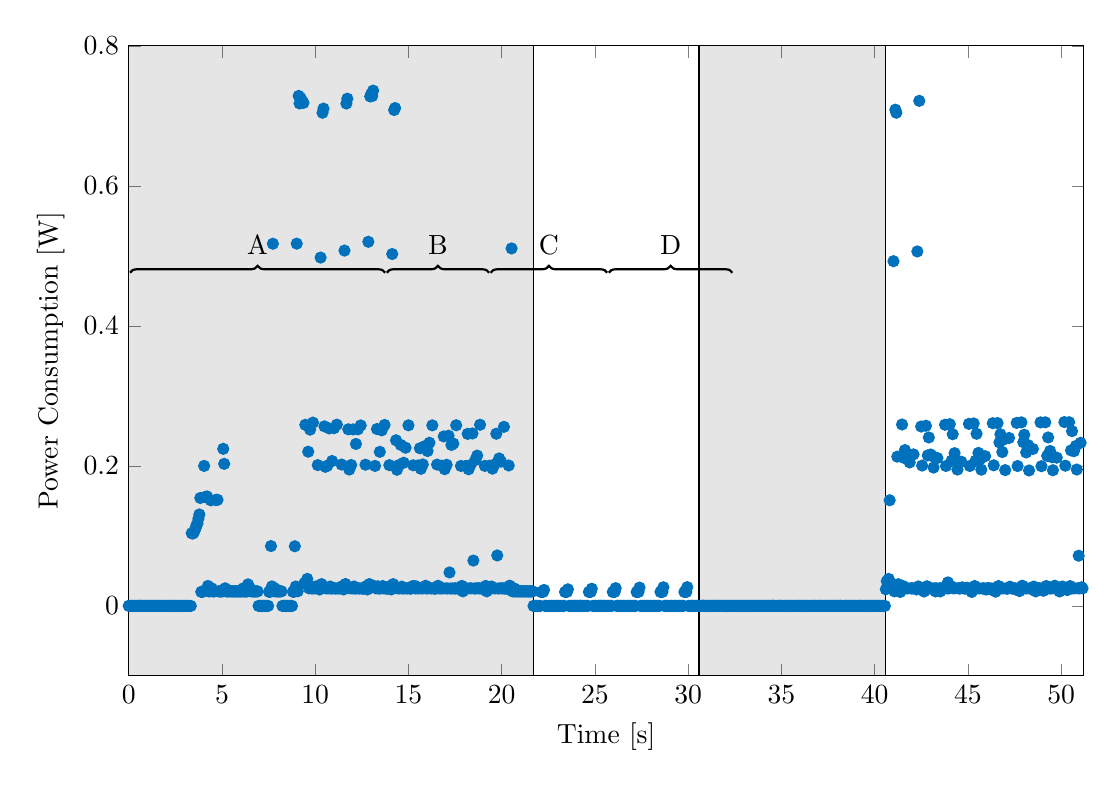
\begin{tikzpicture}

\begin{axis}[%
width=\textwidth,
height=0.66\textwidth,
at={(2.08in,0.858in)},
scale only axis,
xmin=0,
xmax=51.1998976,
xlabel={Time [s]},
ymin=-0.1,
ymax=0.8,
ylabel={Power Consumption [W]},
axis background/.style={fill=white},
%title style={font=\bfseries},
%title={$\text{PSM}_\text{N}\text{BIoTQuectel}_\text{T}\text{AU}_\text{\$}\text{1\$}$}
]
\addplot [color=mycolor1,only marks,mark=*,mark options={solid},forget plot]
  table[row sep=crcr]{%
0.0001024	0.000100730376\\
0.0513024	6.3987444e-06\\
0.1025024	1.61611488e-05\\
0.1537024	2.28993588e-05\\
0.2049024	8.967798e-06\\
0.2561024	1.30196088e-05\\
0.3073024	1.35216864e-05\\
0.3585024	3.9259152e-05\\
0.4097024	-3.37455432e-06\\
0.4609024	-2.50484796e-05\\
0.5121024	1.41411096e-05\\
0.5633024	-4.0649724e-05\\
0.6145024	0.000265105332\\
0.6657024	-8.0003592e-05\\
0.7169024	3.08982096e-05\\
0.7681024	4.2739308e-05\\
0.8193024	5.2899012e-05\\
0.8705024	-2.6718156e-05\\
0.9217024	-4.6301616e-05\\
0.9729024	1.33699752e-05\\
1.0241024	3.02209524e-05\\
1.0753024	5.59467e-05\\
1.1265024	4.4152524e-05\\
1.1777024	4.5168408e-05\\
1.2289024	2.74884516e-05\\
1.2801024	2.34131688e-05\\
1.3313024	1.20623976e-05\\
1.3825024	4.78305e-05\\
1.4337024	1.03692528e-05\\
1.4849024	-1.0673514e-05\\
1.5361024	3.55577112e-05\\
1.5873024	5.2583868e-05\\
1.6385024	-2.26780776e-05\\
1.6897024	5.6167128e-06\\
1.7409024	-8.3609496e-06\\
1.7921024	2.77801416e-05\\
1.8433024	-2.02842072e-05\\
1.8945024	3.44496204e-06\\
1.9457024	2.62035072e-05\\
1.9969024	2.70215784e-05\\
2.0481024	9.8437068e-06\\
2.0993024	9.3768336e-06\\
2.1505024	2.202345e-05\\
2.2017024	1.48879368e-05\\
2.2529024	2.2852422e-05\\
2.3041024	2.84691348e-05\\
2.3553024	-2.55505572e-05\\
2.4065024	9.8906472e-06\\
2.4577024	4.0451076e-05\\
2.5089024	-8.2913796e-06\\
2.5601024	-2.49319692e-05\\
2.6113024	-1.34060148e-05\\
2.6625024	1.61494128e-05\\
2.7137024	1.00775628e-05\\
2.7649024	-5.94738e-05\\
2.8161024	-1.77847236e-05\\
2.8673024	-1.09534716e-05\\
2.9185024	5.5991124e-07\\
2.9697024	9.4346712e-06\\
3.0209024	2.33016912e-07\\
3.0721024	-1.21680072e-05\\
3.1233024	2.11944816e-05\\
3.1745024	-2.44081008e-06\\
3.2257024	2.34827388e-05\\
3.2769024	1.79481708e-05\\
3.3281024	-2.90424564e-05\\
3.3793024	0.103864464\\
3.4305024	0.103352112\\
3.4817024	0.104455008\\
3.5329024	0.107675928\\
3.5841024	0.110758824\\
3.6353024	0.115395984\\
3.6865024	0.117880668\\
3.7377024	0.124679448\\
3.7889024	0.13064274\\
3.8401024	0.154161108\\
3.8913024	0.0200584188\\
3.9425024	0.0199371636\\
3.9937024	0.020880702\\
4.0449024	0.199970208\\
4.0961024	0.155603916\\
4.1473024	0.155343636\\
4.1985024	0.156356208\\
4.2497024	0.0285480072\\
4.3009024	0.0207597456\\
4.3521024	0.0208391832\\
4.4033024	0.15083136\\
4.4545024	0.0250282404\\
4.5057024	0.0207703512\\
4.5569024	0.0208668384\\
4.6081024	0.0207972864\\
4.6593024	0.151222212\\
4.7105024	0.151454556\\
4.7617024	0.151535448\\
4.8129024	0.0207819216\\
4.8641024	0.0207587772\\
4.9153024	0.0207394092\\
4.9665024	0.0207600372\\
5.0177024	0.0207053748\\
5.0689024	0.224381484\\
5.1201024	0.20290194\\
5.1713024	0.02517759\\
5.2225024	0.020743056\\
5.2737024	0.02073942\\
5.3249024	0.0208322136\\
5.3761024	0.0208742256\\
5.4273024	0.0208060236\\
5.4785024	0.0208253916\\
5.5297024	0.0209075976\\
5.5809024	0.020738124\\
5.6321024	0.0208274256\\
5.6833024	0.0206970588\\
5.7345024	0.0207894384\\
5.7857024	0.0208783152\\
5.8369024	0.0207801612\\
5.8881024	0.02074509\\
5.9393024	0.0208177092\\
5.9905024	0.0207723276\\
6.0417024	0.0208009548\\
6.0929024	0.0206764776\\
6.1441024	0.0250793172\\
6.1953024	0.0207748584\\
6.2465024	0.020752686\\
6.2977024	0.0207268956\\
6.3489024	0.0207335772\\
6.4001024	0.03079089\\
6.4513024	0.0250467048\\
6.5025024	0.0249816204\\
6.5537024	0.0208406592\\
6.6049024	0.0208646496\\
6.6561024	0.020861946\\
6.7073024	0.020737908\\
6.7585024	0.0206756532\\
6.8097024	0.0207348084\\
6.8609024	0.020821464\\
6.9121024	0.0207543276\\
6.9633024	1.80060048e-05\\
7.0145024	-8.1975024e-06\\
7.0657024	-1.02996828e-05\\
7.1169024	-5.963724e-05\\
7.1681024	-1.99573128e-05\\
7.2193024	-7.2989604e-06\\
7.2705024	4.5320112e-05\\
7.3217024	-4.1887728e-05\\
7.3729024	-2.04476544e-05\\
7.4241024	-2.12766228e-05\\
7.4753024	1.99916784e-05\\
7.5265024	0.0201398832\\
7.5777024	0.0200624724\\
7.6289024	0.085475772\\
7.6801024	0.0278117172\\
7.7313024	0.51729588\\
7.7825024	0.0209310696\\
7.8337024	0.025094088\\
7.8849024	0.0207996444\\
7.9361024	0.0209242368\\
7.9873024	0.0207635184\\
8.0385024	0.0207280224\\
8.0897024	0.0207732564\\
8.1409024	0.0208429272\\
8.1921024	0.0208325628\\
8.2433024	-1.52274024e-05\\
8.2945024	5.5573704e-05\\
8.3457024	2.49780708e-05\\
8.3969024	4.2902784e-05\\
8.4481024	3.44948832e-05\\
8.4993024	-8.759088e-07\\
8.5505024	-1.05611976e-07\\
8.6017024	5.007348e-05\\
8.6529024	-1.3055652e-05\\
8.7041024	3.17045484e-05\\
8.7553024	-6.9251292e-06\\
8.8065024	0.0202142556\\
8.8577024	0.0201304512\\
8.9089024	0.08521992\\
8.9601024	0.0277353216\\
9.0113024	0.51743304\\
9.0625024	0.0208749852\\
9.1137024	0.72843948\\
9.1649024	0.71765892\\
9.2161024	0.7255098\\
9.2673024	0.72017676\\
9.3185024	0.72072612\\
9.3697024	0.71845992\\
9.4209024	0.0324441864\\
9.4721024	0.258669828\\
9.5233024	0.0322068204\\
9.5745024	0.03857724\\
9.6257024	0.22024602\\
9.6769024	0.025017408\\
9.7281024	0.251754516\\
9.7793024	0.0279427284\\
9.8305024	0.0248753304\\
9.8817024	0.261805716\\
9.9329024	0.02501847\\
9.9841024	0.0252559764\\
10.0353024	0.0277994088\\
10.0865024	0.0251101656\\
10.1377024	0.201129264\\
10.1889024	0.0283241628\\
10.2401024	0.0234372708\\
10.2913024	0.49752036\\
10.3425024	0.0311227956\\
10.3937024	0.70438392\\
10.4449024	0.710289\\
10.4961024	0.256461012\\
10.5473024	0.198715464\\
10.5985024	0.0249708168\\
10.6497024	0.200193876\\
10.7009024	0.0250201044\\
10.7521024	0.253512756\\
10.8033024	0.0277290756\\
10.8545024	0.0247244976\\
10.9057024	0.206926236\\
10.9569024	0.0250781796\\
11.0081024	0.253834668\\
11.0593024	0.0249754644\\
11.1105024	0.0248920272\\
11.1617024	0.258876612\\
11.2129024	0.025092972\\
11.2641024	0.0249311592\\
11.3153024	0.0257420664\\
11.3665024	0.0250744608\\
11.4177024	0.201938508\\
11.4689024	0.0283981176\\
11.5201024	0.02354427\\
11.5713024	0.5075226\\
11.6225024	0.0312388704\\
11.6737024	0.71754444\\
11.7249024	0.72447984\\
11.7761024	0.252228672\\
11.8273024	0.194748336\\
11.8785024	0.0250760628\\
11.9297024	0.201239208\\
11.9809024	0.0249131628\\
12.0321024	0.25212906\\
12.0833024	0.0277967448\\
12.1345024	0.0247136328\\
12.1857024	0.231321492\\
12.2369024	0.0250299252\\
12.2881024	0.252189108\\
12.3393024	0.025040322\\
12.3905024	0.0249147972\\
12.4417024	0.257808672\\
12.4929024	0.024984234\\
12.5441024	0.0248834844\\
12.5953024	0.0246883392\\
12.6465024	0.0250800012\\
12.6977024	0.201678984\\
12.7489024	0.0283571712\\
12.8001024	0.023528286\\
12.8513024	0.52008804\\
12.9025024	0.0311971536\\
12.9537024	0.72763812\\
13.0049024	0.73125468\\
13.0561024	0.7282332\\
13.1073024	0.73599228\\
13.1585024	0.0284462928\\
13.2097024	0.199963008\\
13.2609024	0.0250275636\\
13.3121024	0.252655596\\
13.3633024	0.0280109448\\
13.4145024	0.0247579488\\
13.4657024	0.220065408\\
13.5169024	0.0249773688\\
13.5681024	0.250779168\\
13.6193024	0.0283868316\\
13.6705024	0.025046838\\
13.7217024	0.258488604\\
13.7729024	0.0250181316\\
13.8241024	0.0248805432\\
13.8753024	0.0250044732\\
13.9265024	0.0250313256\\
13.9777024	0.201074256\\
14.0289024	0.0285286104\\
14.0801024	0.0235093896\\
14.1313024	0.50262444\\
14.1825024	0.0310548312\\
14.2337024	0.70834356\\
14.2849024	0.71106732\\
14.3361024	0.236550528\\
14.3873024	0.194500368\\
14.4385024	0.0249807348\\
14.4897024	0.201157092\\
14.5409024	0.024991542\\
14.5921024	0.229930344\\
14.6433024	0.0275774508\\
14.6945024	0.0248071428\\
14.7457024	0.204483492\\
14.7969024	0.0250279596\\
14.8481024	0.225947556\\
14.8993024	0.0251199468\\
14.9505024	0.02499876\\
15.0017024	0.257938812\\
15.0529024	0.024894126\\
15.1041024	0.0249275988\\
15.1553024	0.0248282316\\
15.2065024	0.0280489932\\
15.2577024	0.200861964\\
15.3089024	0.0282840264\\
15.3601024	0.0248969952\\
15.4113024	0.027909792\\
15.4625024	0.0251595432\\
15.5137024	0.200646036\\
15.5649024	0.0249630408\\
15.6161024	0.225115596\\
15.6673024	0.195838848\\
15.7185024	0.0249633864\\
15.7697024	0.202101408\\
15.8209024	0.0251929188\\
15.8721024	0.22814172\\
15.9233024	0.0287766504\\
15.9745024	0.0248600808\\
16.0257024	0.22122018\\
16.0769024	0.02514825\\
16.1281024	0.23299758\\
16.1793024	0.025184286\\
16.2305024	0.0250613892\\
16.2817024	0.257886828\\
16.3329024	0.025123014\\
16.3841024	0.0248892804\\
16.4353024	0.024742134\\
16.4865024	0.0249476472\\
16.5377024	0.201858264\\
16.5889024	0.028737756\\
16.6401024	0.0250032528\\
16.6913024	0.0265769568\\
16.7425024	0.0249917724\\
16.7937024	0.200293164\\
16.8449024	0.0249923772\\
16.8961024	0.24207606\\
16.9473024	0.195315444\\
16.9985024	0.0250188696\\
17.0497024	0.201564288\\
17.1009024	0.0249708636\\
17.1521024	0.243078264\\
17.2033024	0.047835936\\
17.2545024	0.0247897152\\
17.3057024	0.229966632\\
17.3569024	0.0250281108\\
17.4081024	0.231857496\\
17.4593024	0.0249288912\\
17.5105024	0.02505861\\
17.5617024	0.258035328\\
17.6129024	0.0249172344\\
17.6641024	0.0249796764\\
17.7153024	0.0248330088\\
17.7665024	0.0250390404\\
17.8177024	0.199898604\\
17.8689024	0.0286031232\\
17.9201024	0.0207958644\\
17.9713024	0.0248804496\\
18.0225024	0.0249631128\\
18.0737024	0.199900584\\
18.1249024	0.024957648\\
18.1761024	0.245730852\\
18.2273024	0.195166764\\
18.2785024	0.0250736076\\
18.3297024	0.201173508\\
18.3809024	0.0251282088\\
18.4321024	0.246340044\\
18.4833024	0.064742652\\
18.5345024	0.0247825692\\
18.5857024	0.208223388\\
18.6369024	0.0250547508\\
18.6881024	0.214684344\\
18.7393024	0.025280676\\
18.7905024	0.025044444\\
18.8417024	0.258745824\\
18.8929024	0.0249422508\\
18.9441024	0.024846696\\
18.9953024	0.0247275648\\
19.0465024	0.025041132\\
19.0977024	0.200000916\\
19.1489024	0.0285531876\\
19.2001024	0.020837286\\
19.2513024	0.0249944868\\
19.3025024	0.0251536392\\
19.3537024	0.200293704\\
19.4049024	0.0250300944\\
19.4561024	0.027684666\\
19.5073024	0.19604916\\
19.5585024	0.0251181324\\
19.6097024	0.201871728\\
19.6609024	0.02500056\\
19.7121024	0.245916972\\
19.7633024	0.072077292\\
19.8145024	0.0248379228\\
19.8657024	0.210613392\\
19.9169024	0.0250853436\\
19.9681024	0.206072748\\
20.0193024	0.025080264\\
20.0705024	0.0250294788\\
20.1217024	0.255735936\\
20.1729024	0.0249529788\\
20.2241024	0.024744204\\
20.2753024	0.0248444172\\
20.3265024	0.025100892\\
20.3777024	0.200587824\\
20.4289024	0.0288904248\\
20.4801024	0.0233222292\\
20.5313024	0.51061248\\
20.5825024	0.020826468\\
20.6337024	0.0207668736\\
20.6849024	0.0248379588\\
20.7361024	0.0207880092\\
20.7873024	0.0207965376\\
20.8385024	0.02080773\\
20.8897024	0.0208891656\\
20.9409024	0.0207718812\\
20.9921024	0.0208333584\\
21.0433024	0.0207813852\\
21.0945024	0.0207937368\\
21.1457024	0.0207734976\\
21.1969024	0.0207887292\\
21.2481024	0.0208559124\\
21.2993024	0.0207612072\\
21.3505024	0.0208209384\\
21.4017024	0.0208446876\\
21.4529024	0.020716668\\
21.5041024	0.02072322\\
21.5553024	0.0207621576\\
21.6065024	0.0208247724\\
21.6577024	0.0207628668\\
21.7089024	1.13616684e-05\\
21.7601024	4.0752828e-06\\
21.8113024	7.0263828e-05\\
21.8625024	-1.43665812e-06\\
21.9137024	-4.8661128e-05\\
21.9649024	4.0940568e-05\\
22.0161024	-2.80148364e-05\\
22.0673024	2.08675872e-05\\
22.1185024	0.0198705564\\
22.1697024	0.020075544\\
22.2209024	0.0200339352\\
22.2721024	0.0228009672\\
22.3233024	5.860962e-05\\
22.3745024	-4.602168e-05\\
22.4257024	-1.79716392e-05\\
22.4769024	2.26889748e-05\\
22.5281024	-1.5134364e-05\\
22.5793024	4.438638e-05\\
22.6305024	8.4774564e-06\\
22.6817024	2.7757512e-05\\
22.7329024	4.6534644e-05\\
22.7841024	-6.1575984e-05\\
22.8353024	-4.4760204e-05\\
22.8865024	4.004874e-06\\
22.9377024	-8.326584e-06\\
22.9889024	9.1225296e-05\\
23.0401024	-1.54143216e-05\\
23.0913024	3.7286064e-05\\
23.1425024	-4.9618368e-05\\
23.1937024	-1.8310266e-05\\
23.2449024	-9.2485908e-06\\
23.2961024	1.80060048e-05\\
23.3473024	4.9314096e-05\\
23.3985024	0.019914444\\
23.4497024	0.020111976\\
23.5009024	0.0200932524\\
23.5521024	0.0237098052\\
23.6033024	5.7835116e-08\\
23.6545024	-6.5462652e-07\\
23.7057024	-1.60010532e-06\\
23.7569024	1.40589648e-05\\
23.8081024	-3.8688336e-05\\
23.8593024	1.96061112e-05\\
23.9105024	6.4144188e-05\\
23.9617024	5.4650844e-05\\
24.0129024	2.5724898e-05\\
24.0641024	2.00386152e-05\\
24.1153024	1.41411096e-05\\
24.1665024	-1.76095404e-05\\
24.2177024	0.000213723432\\
24.2689024	1.0298844e-05\\
24.3201024	2.65656024e-05\\
24.3713024	1.13382e-05\\
24.4225024	2.42823744e-06\\
24.4737024	4.23873e-06\\
24.5249024	-1.18763172e-05\\
24.5761024	2.83727412e-06\\
24.6273024	2.07971784e-05\\
24.6785024	0.0199057536\\
24.7297024	0.0202195764\\
24.7809024	0.0201283704\\
24.8321024	0.0245727252\\
24.8833024	-3.3245982e-05\\
24.9345024	1.66984272e-05\\
24.9857024	-1.413189e-06\\
25.0369024	6.1738596e-05\\
25.0881024	3.22284168e-06\\
25.1393024	-6.6326004e-06\\
25.1905024	9.1786032e-05\\
25.2417024	3.15159552e-07\\
25.2929024	0.00025669746\\
25.3441024	2.50359048e-05\\
25.3953024	1.06374744e-05\\
25.4465024	4.1373072e-05\\
25.4977024	7.1279712e-05\\
25.5489024	2.54558412e-06\\
25.6001024	1.50052824e-05\\
25.6513024	-1.99916784e-05\\
25.7025024	1.29584232e-06\\
25.7537024	2.08550124e-05\\
25.8049024	3.9107448e-05\\
25.8561024	3.21010128e-05\\
25.9073024	-2.92880448e-05\\
25.9585024	0.019897308\\
26.0097024	0.020099412\\
26.0609024	0.0200840652\\
26.1121024	0.0253999296\\
26.1633024	2.0470284e-05\\
26.2145024	7.4421252e-05\\
26.2657024	-1.52550648e-07\\
26.3169024	2.34475344e-05\\
26.3681024	-7.7306292e-06\\
26.4193024	5.049342e-05\\
26.4705024	-5.32737e-05\\
26.5217024	1.43975952e-05\\
26.5729024	7.5428748e-06\\
26.6241024	-4.6862388e-05\\
26.6753024	-6.4691532e-06\\
26.7265024	-5.5354104e-06\\
26.7777024	6.0302772e-05\\
26.8289024	4.9897476e-05\\
26.8801024	4.7642724e-06\\
26.9313024	-4.1350428e-05\\
26.9825024	-9.4003056e-06\\
27.0337024	2.91354948e-05\\
27.0849024	-2.54801484e-05\\
27.1361024	5.8849344e-06\\
27.1873024	-3.27908448e-05\\
27.2385024	0.0198309384\\
27.2897024	0.0200522412\\
27.3409024	0.0201315996\\
27.3921024	0.0261339588\\
27.4433024	-4.0381488e-05\\
27.4945024	4.096404e-05\\
27.5457024	-3.17162844e-05\\
27.5969024	-3.8187936e-06\\
27.6481024	-2.28063204e-05\\
27.6993024	-3.6084096e-06\\
27.7505024	3.7052208e-05\\
27.8017024	8.5009248e-06\\
27.8529024	-4.8229488e-06\\
27.9041024	-4.2647112e-05\\
27.9553024	1.36742364e-05\\
28.0065024	-7.287228e-06\\
28.0577024	-1.03231512e-05\\
28.1089024	-2.94506532e-05\\
28.1601024	3.0185748e-05\\
28.2113024	1.9653048e-05\\
28.2625024	-2.02724712e-05\\
28.3137024	-2.67298884e-05\\
28.3649024	-2.72789028e-05\\
28.4161024	3.50086932e-05\\
28.4673024	4.0451076e-05\\
28.5185024	0.0200019852\\
28.5697024	0.0200021832\\
28.6209024	0.020016684\\
28.6721024	0.0266250456\\
28.7233024	-3.0280464e-05\\
28.7745024	4.599738e-05\\
28.8257024	3.14002872e-05\\
28.8769024	-4.2915348e-05\\
28.9281024	-1.29743496e-05\\
28.9793024	4.009986e-05\\
29.0305024	1.35216864e-05\\
29.0817024	5.0645124e-05\\
29.1329024	-2.25389376e-06\\
29.1841024	2.13461928e-05\\
29.2353024	-1.017144e-05\\
29.2865024	7.261074e-05\\
29.3377024	1.33934436e-05\\
29.3889024	-1.43514936e-05\\
29.4401024	-3.58502364e-05\\
29.4913024	-2.382975e-06\\
29.5425024	4.8017412e-05\\
29.5937024	-2.66016456e-05\\
29.6449024	-9.4631688e-07\\
29.6961024	-1.75869108e-05\\
29.7473024	1.25762076e-05\\
29.7985024	0.0199175004\\
29.8497024	0.0200014524\\
29.9009024	0.0199896948\\
29.9521024	0.0268038396\\
30.0033024	1.85432832e-05\\
30.0545024	2.14509672e-05\\
30.1057024	1.68032016e-05\\
30.1569024	2.23042428e-06\\
30.2081024	0.000183700296\\
30.2593024	-4.526226e-05\\
30.3105024	-1.67805684e-05\\
30.3617024	-2.49437052e-05\\
30.4129024	1.0590534e-05\\
30.4641024	1.09719108e-06\\
30.5153024	5.4008784e-05\\
30.5665024	3.44479464e-05\\
30.6177024	-2.20703904e-05\\
30.6689024	6.0021972e-05\\
30.7201024	3.10381884e-05\\
30.7713024	5.579496e-05\\
30.8225024	0.00020948472\\
30.8737024	-1.06383132e-05\\
30.9249024	4.8648564e-05\\
30.9761024	8.5596012e-06\\
31.0273024	-2.36595996e-05\\
31.0785024	-9.634158e-06\\
31.1297024	1.8169452e-05\\
31.1809024	-1.96304184e-05\\
31.2321024	-7.636752e-06\\
31.2833024	4.729068e-06\\
31.3345024	9.0418932e-05\\
31.3857024	3.6993528e-05\\
31.4369024	1.70714232e-05\\
31.4881024	3.02209524e-05\\
31.5393024	0.000159083496\\
31.5905024	2.641473e-05\\
31.6417024	3.42149292e-05\\
31.6929024	1.84619808e-05\\
31.7441024	8.6530572e-05\\
31.7953024	2.40200208e-05\\
31.8465024	1.17472356e-05\\
31.8977024	-3.25804572e-06\\
31.9489024	-3.1623246e-05\\
32.0001024	-4.740804e-06\\
32.0513024	-3.6119304e-05\\
32.1025024	-2.173176e-05\\
32.1537024	2.78857548e-05\\
32.2049024	3.7893744e-05\\
32.2561024	2.9134656e-05\\
32.3073024	3.0396132e-05\\
32.3585024	3.29299812e-05\\
32.4097024	3.45418236e-05\\
32.4609024	2.21868972e-06\\
32.5121024	4.6359468e-05\\
32.5633024	-6.3995832e-06\\
32.6145024	-8.664372e-06\\
32.6657024	-1.11169188e-05\\
32.7169024	-3.01329432e-06\\
32.7681024	2.86443144e-05\\
32.8193024	-3.08403756e-05\\
32.8705024	5.4312228e-05\\
32.9217024	-3.04765992e-06\\
32.9729024	-2.73250044e-06\\
33.0241024	4.4129052e-05\\
33.0753024	-2.50954164e-05\\
33.1265024	1.30665492e-05\\
33.1777024	-2.18256372e-05\\
33.2289024	1.21789044e-05\\
33.2801024	-7.9644852e-06\\
33.3313024	4.529664e-05\\
33.3825024	2.09371572e-05\\
33.4337024	-7.053372e-06\\
33.4849024	6.1902036e-05\\
33.5361024	1.99656936e-06\\
33.5873024	-1.81937592e-05\\
33.6385024	9.8671752e-06\\
33.6897024	3.11722992e-06\\
33.7409024	-3.9925512e-05\\
33.7921024	5.157972e-05\\
33.8433024	-3.59432784e-05\\
33.8945024	1.12334256e-05\\
33.9457024	1.06282548e-06\\
33.9969024	-2.96845092e-05\\
34.0481024	-1.5540048e-06\\
34.0993024	2.00729808e-05\\
34.1505024	5.2291332e-05\\
34.2017024	-4.8346812e-06\\
34.2529024	-2.49780708e-05\\
34.3041024	6.6970584e-05\\
34.3553024	-3.20197068e-05\\
34.4065024	2.19647772e-05\\
34.4577024	-9.6919956e-06\\
34.5089024	3.56398524e-05\\
34.5601024	0.000347455872\\
34.6113024	3.7870272e-05\\
34.6625024	1.4944932e-06\\
34.7137024	1.99212696e-05\\
34.7649024	-1.63371672e-05\\
34.8161024	4.4922816e-05\\
34.8673024	3.86523e-05\\
34.9185024	0.000262034208\\
34.9697024	-3.59667468e-06\\
35.0209024	-3.7613808e-05\\
35.0721024	-2.7162396e-05\\
35.1233024	1.44327996e-05\\
35.1745024	-2.5597494e-05\\
35.2257024	3.7612944e-05\\
35.2769024	1.95591708e-05\\
35.3281024	1.88123436e-05\\
35.3793024	-4.2504624e-06\\
35.4305024	-1.16776692e-05\\
35.4817024	-9.0734112e-06\\
35.5329024	2.84926032e-05\\
35.5841024	-1.15846272e-05\\
35.6353024	-1.81585548e-05\\
35.6865024	-1.33004052e-05\\
35.7377024	4.070754e-05\\
35.7889024	-1.15611588e-05\\
35.8401024	5.2981164e-05\\
35.8913024	2.04350796e-06\\
35.9425024	4.2506316e-05\\
35.9937024	6.4086372e-05\\
36.0449024	-9.8562816e-06\\
36.0961024	6.5269872e-06\\
36.1473024	3.10616568e-05\\
36.1985024	1.0076724e-05\\
36.2497024	-5.7566916e-06\\
36.3009024	-4.3149204e-05\\
36.3521024	-1.104651e-05\\
36.4033024	2.9065086e-05\\
36.4545024	-2.67298884e-05\\
36.5057024	9.303912e-08\\
36.5569024	2.8563012e-05\\
36.6081024	-2.42890776e-05\\
36.6593024	2.19061044e-05\\
36.7105024	-1.49826528e-05\\
36.7617024	0.000127787976\\
36.8129024	3.6421884e-05\\
36.8641024	2.96258364e-05\\
36.9153024	4.1256576e-05\\
36.9665024	-1.91627064e-05\\
37.0177024	2.82478536e-05\\
37.0689024	7.3977012e-05\\
37.1201024	-3.7882008e-05\\
37.1713024	-1.31143248e-05\\
37.2225024	-2.04359184e-05\\
37.2737024	-9.7280352e-06\\
37.3249024	-3.33515916e-05\\
37.3761024	-5.6049804e-06\\
37.4273024	8.5269096e-05\\
37.4785024	-6.0844248e-06\\
37.5297024	-1.09417356e-05\\
37.5809024	-1.149075e-05\\
37.6321024	4.8741588e-05\\
37.6833024	-1.9653048e-05\\
37.7345024	5.238522e-05\\
37.7857024	-4.401252e-05\\
37.8369024	3.7706004e-05\\
37.8881024	3.46843152e-06\\
37.9393024	5.5970172e-05\\
37.9905024	-9.1555524e-06\\
38.0417024	1.44914724e-05\\
38.0929024	1.3416912e-05\\
38.1441024	0.000301703256\\
38.1953024	4.1361336e-05\\
38.2465024	-3.9705084e-06\\
38.2977024	1.43749656e-05\\
38.3489024	1.4525838e-05\\
38.4001024	-1.38376836e-05\\
38.4513024	0.000108870012\\
38.5025024	-1.65123504e-05\\
38.5537024	2.52211464e-06\\
38.6049024	6.342084e-05\\
38.6561024	-2.11014396e-05\\
38.7073024	4.7772648e-05\\
38.7585024	-4.7714832e-05\\
38.8097024	-1.98399636e-05\\
38.8609024	1.631286e-05\\
38.9121024	4.0979124e-06\\
38.9633024	1.27513908e-05\\
39.0145024	4.1339556e-06\\
39.0657024	-8.3257452e-06\\
39.1169024	-3.22887672e-05\\
39.1681024	0.00011063358\\
39.2193024	8.6063688e-05\\
39.2705024	5.33592e-06\\
39.3217024	7.35093e-07\\
39.3729024	9.5050764e-06\\
39.4241024	2.40904296e-05\\
39.4753024	1.631286e-05\\
39.5265024	7.0407972e-06\\
39.5777024	1.88349732e-05\\
39.6289024	5.0703804e-05\\
39.6801024	-1.19693592e-05\\
39.7313024	-2.78748576e-05\\
39.7825024	-1.75517064e-05\\
39.8337024	3.26382912e-05\\
39.8849024	2.30510736e-05\\
39.9361024	-3.8512332e-05\\
39.9873024	-8.6417424e-07\\
40.0385024	4.0357188e-05\\
40.0897024	-1.6235748e-06\\
40.1409024	4.6674612e-05\\
40.1921024	-5.0450688e-06\\
40.2433024	7.0041708e-05\\
40.2945024	4.4538084e-05\\
40.3457024	1.32417324e-05\\
40.3969024	-1.87654032e-05\\
40.4481024	-2.53284336e-05\\
40.4993024	-5.2386048e-05\\
40.5505024	-3.52039932e-08\\
40.6017024	0.0237689316\\
40.6529024	0.0352633392\\
40.7041024	0.03475071\\
40.7553024	0.038573856\\
40.8065024	0.150915492\\
40.8577024	0.0282501036\\
40.9089024	0.0249537996\\
40.9601024	0.0308980944\\
41.0113024	0.49237056\\
41.0625024	0.0208366236\\
41.1137024	0.7087554\\
41.1649024	0.70438392\\
41.2161024	0.213219072\\
41.2673024	0.031039758\\
41.3185024	0.0249676632\\
41.3697024	0.0199263672\\
41.4209024	0.0246877056\\
41.4721024	0.259106472\\
41.5233024	0.028401246\\
41.5745024	0.211422996\\
41.6257024	0.222590556\\
41.6769024	0.0249585516\\
41.7281024	0.216969408\\
41.7793024	0.0250562808\\
41.8305024	0.214402824\\
41.8817024	0.204967368\\
41.9329024	0.0251224632\\
41.9841024	0.0250012944\\
42.0353024	0.0250479612\\
42.0865024	0.216435816\\
42.1377024	0.0252040752\\
42.1889024	0.025006572\\
42.2401024	0.0234830124\\
42.2913024	0.50628672\\
42.3425024	0.0278242308\\
42.3937024	0.7213896\\
42.4449024	0.0250898256\\
42.4961024	0.256245804\\
42.5473024	0.200483496\\
42.5985024	0.025014312\\
42.6497024	0.0205779348\\
42.7009024	0.0250394076\\
42.7521024	0.257317956\\
42.8033024	0.0280414188\\
42.8545024	0.215029116\\
42.9057024	0.240606612\\
42.9569024	0.02496078\\
43.0081024	0.2162124\\
43.0593024	0.0250720452\\
43.1105024	0.213630588\\
43.1617024	0.197622468\\
43.2129024	0.025209432\\
43.2641024	0.0207637632\\
43.3153024	0.0251222904\\
43.3665024	0.21116772\\
43.4177024	0.0223375212\\
43.4689024	0.0251562024\\
43.5201024	0.0207539568\\
43.5713024	0.0249911784\\
43.6225024	0.0249281784\\
43.6737024	0.0256452876\\
43.7249024	0.0250511688\\
43.7761024	0.258744276\\
43.8273024	0.199863324\\
43.8785024	0.0249711012\\
43.9297024	0.0335998764\\
43.9809024	0.0250047252\\
44.0321024	0.259521552\\
44.0833024	0.0283496364\\
44.1345024	0.207570348\\
44.1857024	0.245236932\\
44.2369024	0.0250508988\\
44.2881024	0.218184912\\
44.3393024	0.025380504\\
44.3905024	0.20673342\\
44.4417024	0.194773284\\
44.4929024	0.025151346\\
44.5441024	0.0250025148\\
44.5953024	0.0249987168\\
44.6465024	0.206025372\\
44.6977024	0.0265422996\\
44.7489024	0.0252769752\\
44.8001024	0.0248701032\\
44.8513024	0.024963732\\
44.9025024	0.0248968728\\
44.9537024	0.0259568352\\
45.0049024	0.025011162\\
45.0561024	0.260003628\\
45.1073024	0.199876356\\
45.1585024	0.0250652952\\
45.2097024	0.019967994\\
45.2609024	0.0250984692\\
45.3121024	0.260623692\\
45.3633024	0.0283997268\\
45.4145024	0.207298116\\
45.4657024	0.245870676\\
45.5169024	0.0251386704\\
45.5681024	0.218518056\\
45.6193024	0.0249492888\\
45.6705024	0.209956932\\
45.7217024	0.194605668\\
45.7729024	0.0249645204\\
45.8241024	0.0249896196\\
45.8753024	0.0250003908\\
45.9265024	0.213900372\\
45.9777024	0.0234063288\\
46.0289024	0.0251808948\\
46.0801024	0.0249995664\\
46.1313024	0.0253232424\\
46.1825024	0.0248536872\\
46.2337024	0.0234335628\\
46.2849024	0.0249253992\\
46.3361024	0.2610009\\
46.3873024	0.200819556\\
46.4385024	0.0251097732\\
46.4897024	0.0203538276\\
46.5409024	0.0248806188\\
46.5921024	0.261136008\\
46.6433024	0.0283485024\\
46.6945024	0.233512416\\
46.7457024	0.245194704\\
46.7969024	0.0250071048\\
46.8481024	0.219806568\\
46.8993024	0.0249655428\\
46.9505024	0.238044312\\
47.0017024	0.19396134\\
47.0529024	0.024915222\\
47.1041024	0.02454768\\
47.1553024	0.0251011404\\
47.2065024	0.239855292\\
47.2577024	0.0275245596\\
47.3089024	0.0251288748\\
47.3601024	0.0250846416\\
47.4113024	0.0250768224\\
47.4625024	0.0249492312\\
47.5137024	0.0240889896\\
47.5649024	0.0251528688\\
47.6161024	0.261371196\\
47.6673024	0.199791504\\
47.7185024	0.0248689404\\
47.7697024	0.0211933728\\
47.8209024	0.0251396712\\
47.8721024	0.262160856\\
47.9233024	0.0288355716\\
47.9745024	0.233811936\\
48.0257024	0.244437408\\
48.0769024	0.0250313544\\
48.1281024	0.219193488\\
48.1793024	0.0250138656\\
48.2305024	0.229652028\\
48.2817024	0.193446504\\
48.3329024	0.0251859276\\
48.3841024	0.0242562924\\
48.4353024	0.025034922\\
48.4865024	0.224154612\\
48.5377024	0.0276385248\\
48.5889024	0.0249833808\\
48.6401024	0.0207558396\\
48.6913024	0.0250919136\\
48.7425024	0.0249856092\\
48.7937024	0.0251777916\\
48.8449024	0.0250507368\\
48.8961024	0.262145628\\
48.9473024	0.19952352\\
48.9985024	0.0251896572\\
49.0497024	0.0216344268\\
49.1009024	0.0249697872\\
49.1521024	0.262220688\\
49.2033024	0.028406088\\
49.2545024	0.214270812\\
49.3057024	0.24061068\\
49.3569024	0.0249733512\\
49.4081024	0.221317092\\
49.4593024	0.0249037164\\
49.5105024	0.212406336\\
49.5617024	0.193782636\\
49.6129024	0.0250553592\\
49.6641024	0.0288417168\\
49.7153024	0.0250437744\\
49.7665024	0.211756356\\
49.8177024	0.0262041156\\
49.8689024	0.0251067888\\
49.9201024	0.0206385624\\
49.9713024	0.0250043724\\
50.0225024	0.0248790168\\
50.0737024	0.027664542\\
50.1249024	0.0250556652\\
50.1761024	0.2625822\\
50.2273024	0.200288016\\
50.2785024	0.024805008\\
50.3297024	0.0226017\\
50.3809024	0.0251095176\\
50.4321024	0.262350576\\
50.4833024	0.0283451364\\
50.5345024	0.222107904\\
50.5857024	0.249648876\\
50.6369024	0.0250437528\\
50.6881024	0.22104378\\
50.7393024	0.025081398\\
50.7905024	0.228362688\\
50.8417024	0.1948176\\
50.8929024	0.025153974\\
50.9441024	0.07169256\\
50.9953024	0.0250504092\\
51.0465024	0.232958016\\
51.0977024	0.0266505552\\
51.1489024	0.0250756236\\
};

\addplot[area legend,solid,draw=black,fill=black,fill opacity=0.1,forget plot]
table[row sep=crcr] {%
x	y\\
0	-0.1\\
0	0.8\\
21.685	0.8\\
21.685	-0.1\\
}--cycle;

\addplot[area legend,solid,draw=black,fill=black,fill opacity=0.1,forget plot]
table[row sep=crcr] {%
x	y\\
30.582	-0.1\\
30.582	0.8\\
40.563	0.8\\
40.563	-0.1\\
}--cycle;
\end{axis}

\draw [thick,decoration={brace,raise=-0.6cm},decorate]
   (5.3,7.9) -- (8.54,7.9) node [pos=0.5,anchor=north] {A};
\draw [thick,decoration={brace,raise=-0.6cm},decorate]
   (8.56,7.9) -- (9.86,7.9) node [pos=0.5,anchor=north] {B};
\draw [thick,decoration={brace,raise=-0.6cm},decorate]
   (9.88,7.9) -- (11.36,7.9) node [pos=0.5,anchor=north] {C};
\draw [thick,decoration={brace,raise=-0.6cm},decorate]
   (11.38,7.9) -- (12.95,7.9) node [pos=0.5,anchor=north] {D};
   
\end{tikzpicture}%}
\caption{Raw measurement of \gls{PSM}. Area A is connection phase, area B is DRX phase, area C is the PSM phase and area D is the tracking area update phase.}
\label{fig:PSM}
\end{figure}
\end{minipage}
\vspace{1em}
\begin{figure}[H]
\tikzsetnextfilename{eDRX1}
\centering
\begin{minipage}{0.48\textwidth}
\resizebox{\textwidth}{!}{
% This file was created by matlab2tikz.
%
%The latest updates can be retrieved from
%  http://www.mathworks.com/matlabcentral/fileexchange/22022-matlab2tikz-matlab2tikz
%where you can also make suggestions and rate matlab2tikz.
%
\definecolor{mycolor1}{rgb}{0.00000,0.44700,0.74100}%
%
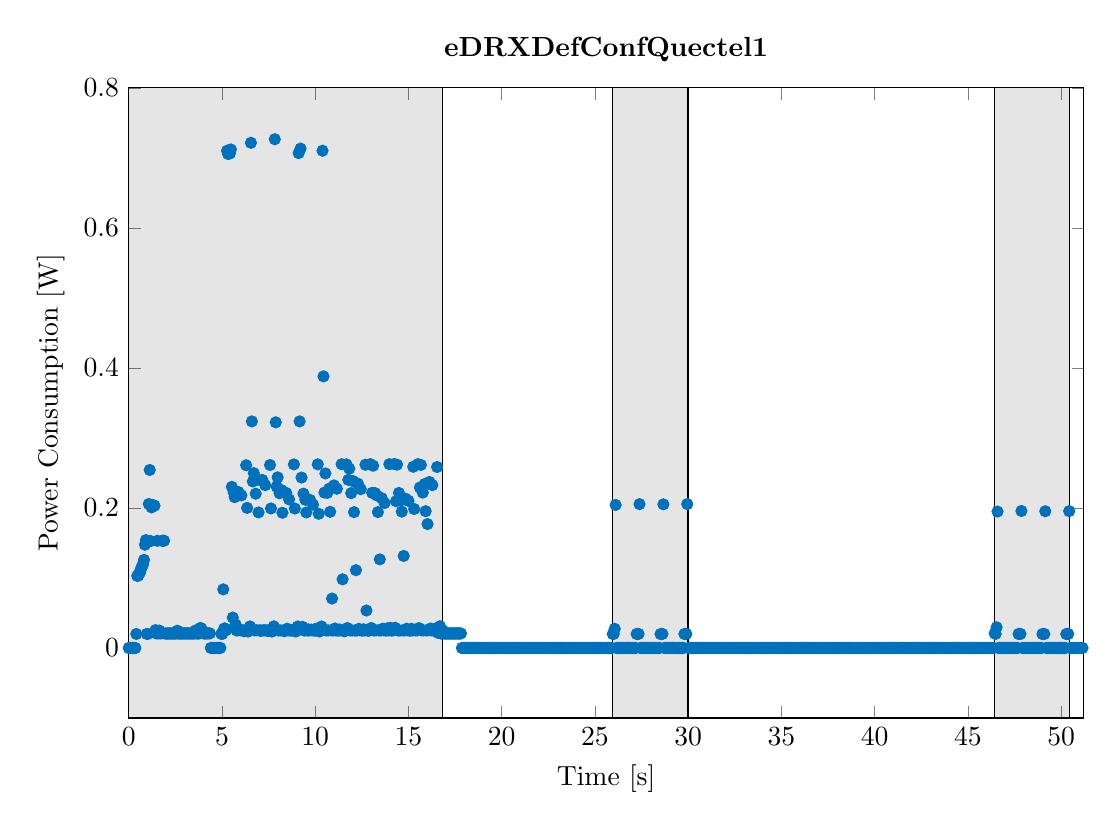
\begin{tikzpicture}

\begin{axis}[%
width=\textwidth,
height=0.66\textwidth,
at={(2.08in,0.858in)},
scale only axis,
xmin=0,
xmax=51.1998976,
xlabel={Time [s]},
ymin=-0.1,
ymax=0.8,
ylabel={Power Consumption [W]},
axis background/.style={fill=white},
title style={font=\bfseries},
title={eDRXDefConfQuectel1}
]
\addplot [color=mycolor1,only marks,mark=*,mark options={solid},forget plot]
  table[row sep=crcr]{%
0.0001024	7.7029704e-07\\
0.0513024	1.24940664e-05\\
0.1025024	-2.18491056e-05\\
0.1537024	3.7333008e-05\\
0.2049024	-1.40715396e-05\\
0.2561024	7.1350128e-05\\
0.3073024	-2.9229372e-05\\
0.3585024	-2.80031004e-05\\
0.4097024	0.0199919736\\
0.4609024	0.102939084\\
0.5121024	0.103248576\\
0.5633024	0.106699824\\
0.6145024	0.108234252\\
0.6657024	0.113970996\\
0.7169024	0.11649294\\
0.7681024	0.119489112\\
0.8193024	0.125794224\\
0.8705024	0.14745726\\
0.9217024	0.154090044\\
0.9729024	0.020089962\\
1.0241024	0.019979046\\
1.0753024	0.20567358\\
1.1265024	0.25423038\\
1.1777024	0.152694432\\
1.2289024	0.200813436\\
1.2801024	0.204115356\\
1.3313024	0.203274576\\
1.3825024	0.203266476\\
1.4337024	0.0254531664\\
1.4849024	0.02071917\\
1.5361024	0.153060984\\
1.5873024	0.0208186056\\
1.6385024	0.0248926176\\
1.6897024	0.0208589364\\
1.7409024	0.0208804428\\
1.7921024	0.153088632\\
1.8433024	0.153103392\\
1.8945024	0.15318108\\
1.9457024	0.0205936272\\
1.9969024	0.0206871588\\
2.0481024	0.0206399484\\
2.0993024	0.020726964\\
2.1505024	0.0207921456\\
2.2017024	0.0208234728\\
2.2529024	0.0207169452\\
2.3041024	0.0207289044\\
2.3553024	0.0208390104\\
2.4065024	0.0207935208\\
2.4577024	0.0206852508\\
2.5089024	0.0207536436\\
2.5601024	0.0207819828\\
2.6113024	0.0246643092\\
2.6625024	0.0207312264\\
2.7137024	0.0206887248\\
2.7649024	0.0207711648\\
2.8161024	0.020741508\\
2.8673024	0.0207978516\\
2.9185024	0.0207806796\\
2.9697024	0.02071188\\
3.0209024	0.0208756332\\
3.0721024	0.0207344016\\
3.1233024	0.0207605556\\
3.1745024	0.0207926028\\
3.2257024	0.0207366912\\
3.2769024	0.0207922752\\
3.3281024	0.0207094068\\
3.3793024	0.0208351404\\
3.4305024	0.0207739512\\
3.4817024	0.0207603108\\
3.5329024	0.020797146\\
3.5841024	0.0250019316\\
3.6353024	0.0208000476\\
3.6865024	0.0207856764\\
3.7377024	0.02088918\\
3.7889024	0.0208038384\\
3.8401024	0.028506006\\
3.8913024	0.0280209384\\
3.9425024	0.0251486244\\
3.9937024	0.0208765188\\
4.0449024	0.0208602036\\
4.0961024	0.0208050084\\
4.1473024	0.02082897\\
4.1985024	0.020856006\\
4.2497024	0.0209245716\\
4.3009024	0.0208914192\\
4.3521024	0.0208030356\\
4.4033024	4.860162e-05\\
4.4545024	-4.6582416e-05\\
4.5057024	-1.30791204e-05\\
4.5569024	3.55342392e-05\\
4.6081024	8.465724e-06\\
4.6593024	-2.597049e-05\\
4.7105024	4.4514612e-05\\
4.7617024	-6.78582e-05\\
4.8129024	2.00964528e-05\\
4.8641024	2.62973844e-05\\
4.9153024	5.3343252e-05\\
4.9665024	0.020100132\\
5.0177024	0.0200740932\\
5.0689024	0.083704752\\
5.1201024	0.0277630308\\
5.1713024	0.027735606\\
5.2225024	0.0252309132\\
5.2737024	0.7101288\\
5.3249024	0.7056198\\
5.3761024	0.71106732\\
5.4273024	0.70630632\\
5.4785024	0.71202852\\
5.5297024	0.230119272\\
5.5809024	0.043383564\\
5.6321024	0.222184548\\
5.6833024	0.215447292\\
5.7345024	0.0335190564\\
5.7857024	0.0250802352\\
5.8369024	0.0251543052\\
5.8881024	0.222656976\\
5.9393024	0.0264803076\\
5.9905024	0.0252675972\\
6.0417024	0.217936224\\
6.0929024	0.0250614432\\
6.1441024	0.024842106\\
6.1953024	0.0239217588\\
6.2465024	0.0249073668\\
6.2977024	0.260980236\\
6.3489024	0.200060604\\
6.4001024	0.0234902088\\
6.4513024	0.0276438852\\
6.5025024	0.0307504872\\
6.5537024	0.7215498\\
6.6049024	0.323648244\\
6.6561024	0.237851856\\
6.7073024	0.249788916\\
6.7585024	0.0251300556\\
6.8097024	0.22033602\\
6.8609024	0.0253042632\\
6.9121024	0.24031638\\
6.9633024	0.193637052\\
7.0145024	0.0251965296\\
7.0657024	0.0244612728\\
7.1169024	0.024945732\\
7.1681024	0.239956632\\
7.2193024	0.025162686\\
7.2705024	0.0251992836\\
7.3217024	0.23252382\\
7.3729024	0.0250028748\\
7.4241024	0.0249630192\\
7.4753024	0.0244549476\\
7.5265024	0.0250219512\\
7.5777024	0.261335232\\
7.6289024	0.199260576\\
7.6801024	0.0233929548\\
7.7313024	0.027658638\\
7.7825024	0.03092229\\
7.8337024	0.72665388\\
7.8849024	0.32229342\\
7.9361024	0.230351652\\
7.9873024	0.243691632\\
8.0385024	0.025028388\\
8.0897024	0.220980024\\
8.1409024	0.0250960464\\
8.1921024	0.225455436\\
8.2433024	0.193112028\\
8.2945024	0.0250755012\\
8.3457024	0.0238707864\\
8.3969024	0.0250081704\\
8.4481024	0.22136724\\
8.4993024	0.0275557968\\
8.5505024	0.0251262468\\
8.6017024	0.212216652\\
8.6529024	0.0251337276\\
8.7041024	0.0249195852\\
8.7553024	0.0252014004\\
8.8065024	0.0251040888\\
8.8577024	0.262219284\\
8.9089024	0.199160352\\
8.9601024	0.023480262\\
9.0113024	0.0277658388\\
9.0625024	0.0306867456\\
9.1137024	0.70680996\\
9.1649024	0.323626392\\
9.2161024	0.7132644\\
9.2673024	0.243424404\\
9.3185024	0.0301940352\\
9.3697024	0.220417884\\
9.4209024	0.0248028444\\
9.4721024	0.2116323\\
9.5233024	0.193554036\\
9.5745024	0.0249675588\\
9.6257024	0.0265901724\\
9.6769024	0.0249975612\\
9.7281024	0.211396716\\
9.7793024	0.0262931724\\
9.8305024	0.0250708104\\
9.8817024	0.204676452\\
9.9329024	0.0249666804\\
9.9841024	0.024944724\\
10.0353024	0.0274927212\\
10.0865024	0.024913638\\
10.1377024	0.262284624\\
10.1889024	0.19165842\\
10.2401024	0.0235066032\\
10.2913024	0.0277248348\\
10.3425024	0.030685194\\
10.3937024	0.71024328\\
10.4449024	0.38793348\\
10.4961024	0.221931324\\
10.5473024	0.24930036\\
10.5985024	0.0249782148\\
10.6497024	0.221510304\\
10.7009024	0.0251134308\\
10.7521024	0.227558088\\
10.8033024	0.194492052\\
10.8545024	0.0251455212\\
10.9057024	0.07060302\\
10.9569024	0.0249953976\\
11.0081024	0.232209756\\
11.0593024	0.0278158212\\
11.1105024	0.0251230824\\
11.1617024	0.22743396\\
11.2129024	0.0249403572\\
11.2641024	0.0250531452\\
11.3153024	0.0263919852\\
11.3665024	0.0250739352\\
11.4177024	0.26249472\\
11.4689024	0.098069616\\
11.5201024	0.0250649064\\
11.5713024	0.0237451536\\
11.6225024	0.02496267\\
11.6737024	0.26228682\\
11.7249024	0.0284809356\\
11.7761024	0.240172812\\
11.8273024	0.25611696\\
11.8785024	0.0250774416\\
11.9297024	0.221157036\\
11.9809024	0.0249971184\\
12.0321024	0.23838282\\
12.0833024	0.19400508\\
12.1345024	0.0249748884\\
12.1857024	0.1111005\\
12.2369024	0.0249414624\\
12.2881024	0.23473764\\
12.3393024	0.0273118068\\
12.3905024	0.025295166\\
12.4417024	0.226800936\\
12.4929024	0.0249752052\\
12.5441024	0.0249785712\\
12.5953024	0.0266730372\\
12.6465024	0.0250844148\\
12.6977024	0.261697176\\
12.7489024	0.05347422\\
12.8001024	0.0248633712\\
12.8513024	0.0246768516\\
12.9025024	0.0250930368\\
12.9537024	0.262619316\\
13.0049024	0.0284961384\\
13.0561024	0.221588712\\
13.1073024	0.260311896\\
13.1585024	0.0249715584\\
13.2097024	0.221197716\\
13.2609024	0.0251860248\\
13.3121024	0.217806192\\
13.3633024	0.194090868\\
13.4145024	0.0251423604\\
13.4657024	0.126577332\\
13.5169024	0.0249991272\\
13.5681024	0.213997752\\
13.6193024	0.0275242572\\
13.6705024	0.0252109476\\
13.7217024	0.207031644\\
13.7729024	0.0248978664\\
13.8241024	0.02510514\\
13.8753024	0.0280696644\\
13.9265024	0.0250011864\\
13.9777024	0.262548036\\
14.0289024	0.0287131428\\
14.0801024	0.02485197\\
14.1313024	0.0273779316\\
14.1825024	0.0250964604\\
14.2337024	0.262822752\\
14.2849024	0.0288388008\\
14.3361024	0.209629152\\
14.3873024	0.261810756\\
14.4385024	0.025056342\\
14.4897024	0.221395392\\
14.5409024	0.0249345252\\
14.5921024	0.21062286\\
14.6433024	0.194736816\\
14.6945024	0.0250574112\\
14.7457024	0.131423724\\
14.7969024	0.0250040448\\
14.8481024	0.213145776\\
14.8993024	0.027405612\\
14.9505024	0.0252559008\\
15.0017024	0.210145392\\
15.0529024	0.0248484384\\
15.1041024	0.0248762664\\
15.1553024	0.0273844404\\
15.2065024	0.0250223328\\
15.2577024	0.258789744\\
15.3089024	0.198440316\\
15.3601024	0.025107012\\
15.4113024	0.026053686\\
15.4625024	0.0250775568\\
15.5137024	0.262652868\\
15.5649024	0.0283830228\\
15.6161024	0.229168224\\
15.6673024	0.261491148\\
15.7185024	0.025125534\\
15.7697024	0.221919948\\
15.8209024	0.0250911072\\
15.8721024	0.234169272\\
15.9233024	0.195330888\\
15.9745024	0.0250109208\\
16.0257024	0.176981832\\
16.0769024	0.0253520064\\
16.1281024	0.23712912\\
16.1793024	0.027729558\\
16.2305024	0.0251454168\\
16.2817024	0.23259654\\
16.3329024	0.024919002\\
16.3841024	0.0250163244\\
16.4353024	0.02756583\\
16.4865024	0.0250751052\\
16.5377024	0.2584926\\
16.5889024	0.0215791272\\
16.6401024	0.0235818\\
16.6913024	0.0310584312\\
16.7425024	0.0206883\\
16.7937024	0.0207709848\\
16.8449024	0.0249071724\\
16.8961024	0.020835972\\
16.9473024	0.0207620244\\
16.9985024	0.0207497916\\
17.0497024	0.0207797688\\
17.1009024	0.0206956656\\
17.1521024	0.0207864828\\
17.2033024	0.0207225432\\
17.2545024	0.0207333396\\
17.3057024	0.0207816012\\
17.3569024	0.0206705952\\
17.4081024	0.020738808\\
17.4593024	0.020756754\\
17.5105024	0.02070495\\
17.5617024	0.0207342684\\
17.6129024	0.0208696212\\
17.6641024	0.0206948556\\
17.7153024	0.0207305856\\
17.7665024	0.020771784\\
17.8177024	0.0207610128\\
17.8689024	-3.2206626e-05\\
17.9201024	-4.5834768e-05\\
17.9713024	3.9177864e-05\\
18.0225024	6.888582e-05\\
18.0737024	-2.57257368e-05\\
18.1249024	5.0090256e-06\\
18.1761024	8.0449524e-06\\
18.2273024	9.4229352e-06\\
18.2785024	1.54025856e-05\\
18.3297024	1.50538968e-06\\
18.3809024	1.82867976e-05\\
18.4321024	3.6398412e-05\\
18.4833024	3.9808188e-05\\
18.5345024	-3.47522076e-05\\
18.5857024	0.000171077148\\
18.6369024	4.529664e-05\\
18.6881024	2.99175264e-05\\
18.7393024	-3.27673728e-05\\
18.7905024	4.3451784e-05\\
18.8417024	2.53745352e-05\\
18.8929024	-5.842188e-07\\
18.9441024	2.5444944e-05\\
18.9953024	1.29265704e-05\\
19.0465024	-4.4409852e-05\\
19.0977024	-4.483062e-05\\
19.1489024	-4.5312552e-06\\
19.2001024	-1.00079928e-05\\
19.2513024	-5.3132868e-06\\
19.3025024	1.521567e-05\\
19.3537024	1.04044572e-05\\
19.4049024	-8.9921052e-06\\
19.4561024	2.05867908e-05\\
19.5073024	1.90453608e-05\\
19.5585024	-3.8641428e-05\\
19.6097024	-4.145688e-06\\
19.6609024	2.03655096e-05\\
19.7121024	4.751532e-05\\
19.7633024	4.6289052e-05\\
19.8145024	-3.45543948e-05\\
19.8657024	-5.613444e-05\\
19.9169024	-2.03303052e-05\\
19.9681024	3.8605356e-05\\
20.0193024	2.224557e-05\\
20.0705024	-1.4106744e-05\\
20.1217024	-1.11873276e-05\\
20.1729024	-1.91979108e-05\\
20.2241024	-3.9587724e-06\\
20.2753024	3.632886e-05\\
20.3265024	8.4891924e-06\\
20.3777024	-1.59046596e-05\\
20.4289024	5.0995512e-05\\
20.4801024	5.860962e-05\\
20.5313024	-2.09966688e-05\\
20.5825024	4.0182012e-05\\
20.6337024	-1.10976408e-06\\
20.6849024	-2.07510768e-05\\
20.7361024	1.22543424e-06\\
20.7873024	6.2235648e-06\\
20.8385024	2.3074542e-05\\
20.8897024	-3.20783832e-05\\
20.9409024	3.3854508e-06\\
20.9921024	-2.27945844e-05\\
21.0433024	6.1972452e-05\\
21.0945024	-7.5319776e-06\\
21.1457024	1.72591776e-05\\
21.1969024	5.2139628e-05\\
21.2481024	1.2028032e-06\\
21.2993024	3.53355876e-05\\
21.3505024	2.24668548e-05\\
21.4017024	-2.98831608e-05\\
21.4529024	2.15331084e-05\\
21.5041024	4.5063612e-05\\
21.5553024	9.6802596e-06\\
21.6065024	-1.19115216e-05\\
21.6577024	-2.58422472e-05\\
21.7089024	4.849686e-05\\
21.7601024	0.000118258596\\
21.8113024	2.89946808e-05\\
21.8625024	2.84221944e-05\\
21.9137024	3.6561852e-05\\
21.9649024	-8.4665592e-06\\
22.0161024	1.81350864e-05\\
22.0673024	2.08441152e-05\\
22.1185024	-3.4051482e-05\\
22.1697024	-1.6579404e-06\\
22.2209024	1.9956474e-05\\
22.2721024	-1.7060526e-05\\
22.3233024	7.7767308e-06\\
22.3745024	1.6324596e-05\\
22.4257024	3.3628194e-06\\
22.4769024	2.33016912e-07\\
22.5281024	-1.40145408e-06\\
22.5793024	4.4304228e-05\\
22.6305024	3.58024608e-05\\
22.6817024	-1.67923044e-05\\
22.7329024	-3.04263072e-07\\
22.7841024	3.15989352e-05\\
22.8353024	2.6034192e-06\\
22.8865024	4.9886568e-05\\
22.9377024	-4.5787824e-05\\
22.9889024	4.5273168e-05\\
23.0401024	-1.02301128e-05\\
23.0913024	-4.5437472e-05\\
23.1425024	-3.990204e-05\\
23.1937024	0.000168332076\\
23.2449024	3.8605356e-05\\
23.2961024	-8.214264e-08\\
23.3473024	-3.8862684e-05\\
23.3985024	2.30393376e-05\\
23.4497024	1.1572056e-05\\
23.5009024	-1.88123436e-05\\
23.5521024	4.2319404e-05\\
23.6033024	1.27396548e-05\\
23.6545024	-1.40128668e-05\\
23.7057024	1.7060526e-05\\
23.7569024	6.1283448e-05\\
23.8081024	9.2988828e-05\\
23.8593024	-4.1724288e-05\\
23.9105024	1.09526328e-05\\
23.9617024	3.50673696e-05\\
24.0129024	2.92285332e-05\\
24.0641024	5.8982616e-05\\
24.1153024	-2.16269856e-05\\
24.1665024	-5.9318712e-06\\
24.2177024	-5.3727984e-07\\
24.2689024	-2.13470316e-05\\
24.3201024	-1.89640548e-05\\
24.3713024	2.58187752e-05\\
24.4225024	-3.10977e-05\\
24.4737024	2.099583e-05\\
24.5249024	-8.4782952e-06\\
24.5761024	3.1377654e-05\\
24.6273024	6.525396e-05\\
24.6785024	3.8472948e-07\\
24.7297024	-3.55116096e-05\\
24.7809024	4.660506e-05\\
24.8321024	-8.4078864e-06\\
24.8833024	2.08089144e-05\\
24.9345024	0.000175210272\\
24.9857024	-7.789302e-06\\
25.0369024	-4.5425736e-05\\
25.0881024	0.00011821248\\
25.1393024	-1.98516996e-05\\
25.1905024	9.1195092e-06\\
25.2417024	4.9395384e-05\\
25.2929024	4.8519468e-05\\
25.3441024	3.1213368e-05\\
25.3953024	5.8027932e-06\\
25.4465024	1.92205404e-05\\
25.4977024	-6.9133932e-06\\
25.5489024	-1.94896008e-05\\
25.6001024	2.82822192e-05\\
25.6513024	4.7678796e-05\\
25.7025024	7.0290648e-06\\
25.7537024	1.95709068e-05\\
25.8049024	1.73756844e-05\\
25.8561024	2.27585448e-05\\
25.9073024	4.4666316e-05\\
25.9585024	0.0199496628\\
26.0097024	0.020042712\\
26.0609024	0.0273470688\\
26.1121024	0.20430252\\
26.1633024	4.9386168e-06\\
26.2145024	4.6100484e-08\\
26.2657024	5.2782516e-05\\
26.3169024	5.08203e-05\\
26.3681024	1.40128668e-05\\
26.4193024	-3.25108872e-05\\
26.4705024	1.98399636e-05\\
26.5217024	-1.15846272e-05\\
26.5729024	-3.963384e-05\\
26.6241024	1.96178436e-05\\
26.6753024	-3.48016608e-06\\
26.7265024	3.6386676e-05\\
26.7777024	0.000170026056\\
26.8289024	1.79708004e-05\\
26.8801024	2.94204816e-06\\
26.9313024	2.4639444e-05\\
26.9825024	3.46239648e-05\\
27.0337024	-4.8346812e-06\\
27.0849024	-6.1132572e-05\\
27.1361024	-3.9505572e-05\\
27.1873024	3.15159552e-07\\
27.2385024	0.019976724\\
27.2897024	0.0200798568\\
27.3409024	0.0200967876\\
27.3921024	0.205462908\\
27.4433024	3.8664036e-05\\
27.4945024	5.8338036e-07\\
27.5457024	-1.06282548e-06\\
27.5969024	3.8883636e-06\\
27.6481024	-2.64381984e-05\\
27.6993024	1.8671526e-05\\
27.7505024	1.88006076e-05\\
27.8017024	-7.648488e-06\\
27.8529024	-1.12694688e-05\\
27.9041024	-1.36164024e-05\\
27.9553024	3.2252724e-05\\
28.0065024	1.30665492e-05\\
28.0577024	4.3113168e-05\\
28.1089024	1.12216932e-05\\
28.1601024	-3.58619724e-05\\
28.2113024	-4.5986472e-05\\
28.2625024	6.1446888e-05\\
28.3137024	-5.6333088e-05\\
28.3649024	-7.6375908e-06\\
28.4161024	4.3521372e-05\\
28.4673024	1.30078764e-05\\
28.5185024	0.019892718\\
28.5697024	0.0200542176\\
28.6209024	0.0200350224\\
28.6721024	0.205180488\\
28.7233024	2.07267696e-05\\
28.7745024	7.986276e-06\\
28.8257024	-5.5784088e-05\\
28.8769024	4.493538e-05\\
28.9281024	-9.3458232e-07\\
28.9793024	-1.07456004e-06\\
29.0305024	-3.03969708e-05\\
29.0817024	-3.44839896e-05\\
29.1329024	2.66360112e-05\\
29.1841024	0.000189970812\\
29.2353024	-1.81007208e-05\\
29.2865024	1.4970078e-05\\
29.3377024	-2.72076588e-06\\
29.3889024	-2.11710096e-05\\
29.4401024	-4.2249816e-05\\
29.4913024	6.4319364e-05\\
29.5425024	-1.16307288e-05\\
29.5937024	-3.9505572e-05\\
29.6449024	2.82361176e-05\\
29.6961024	-1.2845268e-05\\
29.7473024	5.5654992e-05\\
29.7985024	0.0199372536\\
29.8497024	0.0201271572\\
29.9009024	0.0200915352\\
29.9521024	0.205534368\\
30.0033024	3.768336e-05\\
30.0545024	-9.9023796e-06\\
30.1057024	-9.2024928e-06\\
30.1569024	0.00021262626\\
30.2081024	-9.5059152e-06\\
30.2593024	-4.6360296e-06\\
30.3105024	-3.43322748e-05\\
30.3617024	-2.8481706e-05\\
30.4129024	2.53519056e-05\\
30.4641024	-2.76292692e-05\\
30.5153024	6.2649684e-05\\
30.5665024	4.5869112e-05\\
30.6177024	6.0793092e-05\\
30.6689024	-2.37878424e-05\\
30.7201024	-1.48359672e-06\\
30.7713024	-3.09459852e-05\\
30.8225024	2.6764254e-05\\
30.8737024	-1.25887788e-05\\
30.9249024	-2.10897072e-05\\
30.9761024	1.24127604e-05\\
31.0273024	3.7566e-05\\
31.0785024	-1.22627232e-06\\
31.1297024	-7.0651044e-06\\
31.1809024	9.3174912e-05\\
31.2321024	3.9749508e-05\\
31.2833024	-2.06697744e-06\\
31.3345024	-5.0096952e-05\\
31.3857024	2.22916716e-05\\
31.4369024	-1.156032e-05\\
31.4881024	-1.59281316e-05\\
31.5393024	4.5890928e-06\\
31.5905024	5.5281168e-05\\
31.6417024	-2.49898068e-05\\
31.6929024	4.1683212e-06\\
31.7441024	4.1676516e-05\\
31.7953024	1.68853428e-05\\
31.8465024	-1.95046884e-06\\
31.8977024	1.77847236e-05\\
31.9489024	5.5385928e-05\\
32.0001024	-1.47957372e-05\\
32.0513024	-2.74188816e-05\\
32.1025024	-7.6836924e-06\\
32.1537024	3.9563424e-05\\
32.2049024	3.41101548e-05\\
32.2561024	-1.65584484e-05\\
32.3073024	-3.5231652e-05\\
32.3585024	2.61691416e-05\\
32.4097024	-1.79833716e-05\\
32.4609024	3.05939448e-06\\
32.5121024	6.5499552e-05\\
32.5633024	-2.04350796e-06\\
32.6145024	-2.7911736e-06\\
32.6657024	1.99212696e-05\\
32.7169024	7.6602204e-06\\
32.7681024	3.15159552e-07\\
32.8193024	4.2284196e-05\\
32.8705024	3.23927028e-05\\
32.9217024	-1.73765232e-05\\
32.9729024	2.53049652e-05\\
33.0241024	-1.5122628e-05\\
33.0753024	-3.15763056e-05\\
33.1265024	6.2470332e-06\\
33.1777024	-1.84393476e-05\\
33.2289024	-1.0451394e-05\\
33.2801024	-9.3877308e-08\\
33.3313024	3.53355876e-05\\
33.3825024	-3.713184e-06\\
33.4337024	1.28561616e-05\\
33.4849024	-5.0809428e-05\\
33.5361024	1.76908464e-05\\
33.5873024	3.9344652e-06\\
33.6385024	-3.83841e-05\\
33.6897024	3.06643536e-05\\
33.7409024	2.9660202e-05\\
33.7921024	3.24631116e-06\\
33.8433024	-3.643614e-06\\
33.8945024	-3.14706924e-05\\
33.9457024	2.88077616e-05\\
33.9969024	-1.70261604e-05\\
34.0481024	-4.2039432e-05\\
34.0993024	1.53204444e-05\\
34.1505024	3.5685954e-05\\
34.2017024	1.12099572e-05\\
34.2529024	1.50748524e-05\\
34.3041024	6.2860068e-05\\
34.3553024	3.5685954e-05\\
34.4065024	-3.19032e-05\\
34.4577024	-1.413189e-06\\
34.5089024	4.4013384e-06\\
34.5601024	6.374772e-05\\
34.6113024	-1.29500388e-05\\
34.6625024	5.7395088e-05\\
34.7137024	4.9594032e-05\\
34.7649024	-4.7925216e-05\\
34.8161024	2.79092232e-05\\
34.8673024	9.2946924e-06\\
34.9185024	2.1813066e-05\\
34.9697024	3.9819924e-05\\
35.0209024	-1.66523256e-05\\
35.0721024	-3.27673728e-05\\
35.1233024	-1.45040436e-05\\
35.1745024	2.3062806e-05\\
35.2257024	1.34873208e-05\\
35.2769024	5.5991124e-07\\
35.3281024	-4.8065184e-05\\
35.3793024	0.000108531396\\
35.4305024	2.9963628e-05\\
35.4817024	5.6379204e-05\\
35.5329024	-6.014016e-06\\
35.5841024	-1.70144244e-05\\
35.6353024	-3.18562596e-05\\
35.6865024	-2.62512828e-05\\
35.7377024	2.18834712e-05\\
35.7889024	-3.8559276e-05\\
35.8401024	-1.8042048e-05\\
35.8913024	1.8917118e-05\\
35.9425024	-4.2249816e-05\\
35.9937024	-4.2974028e-06\\
36.0449024	3.45996576e-05\\
36.0961024	3.8033712e-05\\
36.1473024	4.924368e-05\\
36.1985024	-3.183363e-05\\
36.2497024	0.000188032896\\
36.3009024	-1.63019628e-05\\
36.3521024	6.2352972e-06\\
36.4033024	6.8594148e-05\\
36.4545024	-9.9149544e-06\\
36.5057024	-2.37291696e-05\\
36.5569024	3.0933414e-05\\
36.6081024	5.091336e-05\\
36.6593024	2.5947018e-05\\
36.7105024	0.000116203356\\
36.7617024	2.24090172e-05\\
36.8129024	-6.4530612e-05\\
36.8641024	2.41952004e-05\\
36.9153024	-9.4915836e-05\\
36.9665024	3.9270888e-05\\
37.0177024	5.5012932e-05\\
37.0689024	2.1952206e-06\\
37.1201024	-5.6146176e-05\\
37.1713024	3.44412396e-06\\
37.2225024	3.951648e-05\\
37.2737024	4.3451784e-05\\
37.3249024	1.73991564e-05\\
37.3761024	2.09136852e-05\\
37.4273024	-3.15880416e-05\\
37.4785024	6.678702e-06\\
37.5297024	2.9134656e-05\\
37.5809024	2.31675804e-05\\
37.6321024	-2.4838092e-05\\
37.6833024	-4.2160968e-06\\
37.7345024	5.4790812e-05\\
37.7857024	5.5596312e-05\\
37.8369024	2.28758904e-05\\
37.8881024	-1.28570004e-05\\
37.9393024	3.9213072e-05\\
37.9905024	-1.95046884e-06\\
38.0417024	2.47442148e-05\\
38.0929024	-2.74306176e-05\\
38.1441024	1.6838406e-05\\
38.1953024	5.0995512e-05\\
38.2465024	-6.3888552e-05\\
38.2977024	-3.7368216e-05\\
38.3489024	-2.28180564e-05\\
38.4001024	1.33004052e-05\\
38.4513024	-1.45501452e-05\\
38.5025024	1.52969724e-06\\
38.5537024	-2.2548996e-05\\
38.6049024	6.4222128e-06\\
38.6561024	3.8792304e-05\\
38.7073024	8.7243048e-05\\
38.7585024	2.64960324e-05\\
38.8097024	1.02519072e-05\\
38.8609024	-5.8621356e-05\\
38.9121024	-2.1725892e-06\\
38.9633024	1.24479648e-05\\
39.0145024	3.9890304e-05\\
39.0657024	-5.0412132e-05\\
39.1169024	3.1155534e-05\\
39.1681024	-3.7730304e-05\\
39.2193024	1.53087084e-05\\
39.2705024	2.63669544e-05\\
39.3217024	-1.71074628e-05\\
39.3729024	7.077762e-05\\
39.4241024	1.26466164e-05\\
39.4753024	-2.9202552e-06\\
39.5265024	-1.96304184e-05\\
39.5777024	5.1733116e-06\\
39.6289024	1.73924496e-06\\
39.6801024	-2.35657224e-05\\
39.7313024	-1.17480744e-05\\
39.7825024	5.8948236e-05\\
39.8337024	-6.8209416e-05\\
39.8849024	1.87184664e-05\\
39.9361024	1.09291644e-05\\
39.9873024	-2.05289568e-05\\
40.0385024	2.62739124e-05\\
40.0897024	-2.2701546e-05\\
40.1409024	1.93957236e-05\\
40.1921024	0.000114988824\\
40.2433024	-1.697922e-05\\
40.2945024	4.849686e-05\\
40.3457024	9.4003056e-06\\
40.3969024	9.924174e-07\\
40.4481024	-3.8883636e-06\\
40.4993024	1.54143216e-06\\
40.5505024	1.90336248e-05\\
40.6017024	-2.46168108e-05\\
40.6529024	8.0214804e-06\\
40.7041024	-6.4787076e-05\\
40.7553024	-2.25263664e-05\\
40.8065024	5.1905772e-05\\
40.8577024	-2.09731968e-05\\
40.9089024	1.09643688e-05\\
40.9601024	2.69629056e-05\\
41.0113024	0.000252447012\\
41.0625024	-4.8392064e-05\\
41.1137024	-9.5285484e-06\\
41.1649024	-1.52626068e-05\\
41.2161024	1.9442664e-05\\
41.2673024	4.5331848e-05\\
41.3185024	0.000114276348\\
41.3697024	3.0104442e-05\\
41.4209024	4.94658e-05\\
41.4721024	9.5285484e-06\\
41.5233024	0.0002468529\\
41.5745024	4.4689788e-05\\
41.6257024	4.401252e-05\\
41.6769024	1.92616128e-06\\
41.7281024	9.1312452e-06\\
41.7793024	-3.7216476e-05\\
41.8305024	-1.521567e-05\\
41.8817024	-1.39080924e-05\\
41.9329024	-6.7928616e-05\\
41.9841024	1.70714232e-05\\
42.0353024	7.7632344e-05\\
42.0865024	5.8983444e-05\\
42.1377024	1.75156632e-05\\
42.1889024	3.54529368e-05\\
42.2401024	3.57094224e-05\\
42.2913024	4.5471816e-05\\
42.3425024	1.59859656e-05\\
42.3937024	-4.0635468e-06\\
42.4449024	5.8924764e-05\\
42.4961024	-1.499355e-05\\
42.5473024	-1.6032906e-05\\
42.5985024	2.7055944e-05\\
42.6497024	-1.35107892e-05\\
42.7009024	1.73924496e-06\\
42.7521024	4.4782848e-05\\
42.8033024	-5.3612316e-05\\
42.8545024	-1.8264168e-05\\
42.9057024	-4.5612648e-05\\
42.9569024	8.5243968e-06\\
43.0081024	3.6468828e-05\\
43.0593024	5.719644e-05\\
43.1105024	-1.60454772e-05\\
43.1617024	-1.8018576e-05\\
43.2129024	-2.8049202e-05\\
43.2641024	3.9983364e-05\\
43.3153024	6.0513156e-05\\
43.3665024	-9.8914824e-06\\
43.4177024	-3.7022868e-06\\
43.4689024	-2.90424564e-05\\
43.5201024	7.8354036e-06\\
43.5713024	-1.64184732e-05\\
43.6225024	4.2284196e-05\\
43.6737024	1.53556452e-05\\
43.7249024	-4.3326072e-06\\
43.7761024	3.19023612e-05\\
43.8273024	-3.40053804e-05\\
43.8785024	2.47794192e-05\\
43.9297024	-3.6201456e-06\\
43.9809024	3.13298784e-05\\
44.0321024	2.39504508e-05\\
44.0833024	-1.36281348e-05\\
44.1345024	3.2790006e-05\\
44.1857024	3.6071532e-05\\
44.2369024	-1.22493132e-05\\
44.2881024	-6.186852e-05\\
44.3393024	0.000166581108\\
44.3905024	4.5109728e-05\\
44.4417024	-1.9081404e-05\\
44.4929024	1.49583456e-05\\
44.5441024	1.66967496e-06\\
44.5953024	1.46197152e-05\\
44.6465024	-2.36470248e-05\\
44.6977024	1.19106828e-06\\
44.7489024	1.65115116e-05\\
44.8001024	3.03726636e-05\\
44.8513024	-1.11873276e-05\\
44.9025024	0.000231590304\\
44.9537024	7.2981216e-06\\
45.0049024	1.72357092e-05\\
45.0561024	8.120556e-05\\
45.1073024	1.91627064e-05\\
45.1585024	-6.44652e-06\\
45.2097024	3.6526644e-05\\
45.2609024	-3.07238652e-05\\
45.3121024	2.12414184e-05\\
45.3633024	6.4903608e-05\\
45.4145024	-1.00540944e-05\\
45.4657024	3.45300876e-05\\
45.5169024	4.3965612e-05\\
45.5681024	-3.02217912e-05\\
45.6193024	-1.02879468e-05\\
45.6705024	5.0794344e-06\\
45.7217024	3.929436e-05\\
45.7729024	1.78190892e-05\\
45.8241024	-1.30841496e-06\\
45.8753024	2.9310678e-05\\
45.9265024	-1.60446384e-05\\
45.9777024	1.76908464e-05\\
46.0289024	-4.8801132e-05\\
46.0801024	0.000159410376\\
46.1313024	4.3253136e-05\\
46.1825024	-7.5437136e-06\\
46.2337024	0.000128616948\\
46.2849024	3.08982096e-05\\
46.3361024	3.832542e-05\\
46.3873024	4.9034124e-07\\
46.4385024	0.0209229516\\
46.4897024	0.0201117816\\
46.5409024	0.0295496748\\
46.5921024	0.194821128\\
46.6433024	1.46431836e-05\\
46.6945024	4.0427604e-05\\
46.7457024	7.206174e-05\\
46.7969024	-4.2285024e-05\\
46.8481024	4.6651176e-05\\
46.8993024	2.5444944e-05\\
46.9505024	2.12405796e-05\\
47.0017024	-5.8966704e-06\\
47.0529024	2.574837e-05\\
47.1041024	-3.6025416e-05\\
47.1553024	7.3442232e-06\\
47.2065024	5.205834e-05\\
47.2577024	1.8694998e-05\\
47.3089024	2.14828164e-06\\
47.3601024	4.0964868e-05\\
47.4113024	4.1800536e-06\\
47.4625024	1.90336248e-05\\
47.5137024	3.52308168e-05\\
47.5649024	6.9477588e-06\\
47.6161024	-3.28143132e-05\\
47.6673024	3.04765992e-06\\
47.7185024	0.0199704168\\
47.7697024	0.0200516256\\
47.8209024	0.0200953368\\
47.8721024	0.195674472\\
47.9233024	-4.5752616e-05\\
47.9745024	-1.36859724e-05\\
48.0257024	1.49583456e-05\\
48.0769024	-5.3635788e-05\\
48.1281024	3.8079828e-05\\
48.1793024	-2.64616668e-05\\
48.2305024	3.1002984e-05\\
48.2817024	-4.7181744e-06\\
48.3329024	2.34014364e-05\\
48.3841024	-1.88827524e-05\\
48.4353024	2.37283308e-05\\
48.4865024	-2.02255308e-05\\
48.5377024	1.12920984e-05\\
48.5889024	1.660455e-05\\
48.6401024	1.50622812e-06\\
48.6913024	4.718844e-05\\
48.7425024	-4.2039432e-05\\
48.7937024	-2.79209592e-05\\
48.8449024	1.87536708e-05\\
48.8961024	3.6363204e-05\\
48.9473024	7.0760016e-06\\
48.9985024	0.01993203\\
49.0497024	0.0199989108\\
49.1009024	0.0199553652\\
49.1521024	0.1953045\\
49.2033024	-4.846248e-05\\
49.2545024	-2.77943904e-06\\
49.3057024	2.99409948e-05\\
49.3569024	2.87381916e-05\\
49.4081024	4.5424872e-05\\
49.4593024	4.5180144e-05\\
49.5105024	8.6526396e-06\\
49.5617024	-6.2244e-06\\
49.6129024	2.94037164e-05\\
49.6641024	0.00016837902\\
49.7153024	-7.7775696e-06\\
49.7665024	-4.8120516e-06\\
49.8177024	4.7118852e-05\\
49.8689024	4.6312524e-05\\
49.9201024	0.000158301468\\
49.9713024	-2.20360248e-05\\
50.0225024	-6.5982348e-06\\
50.0737024	1.4164578e-05\\
50.1249024	1.04974956e-05\\
50.1761024	1.45928952e-06\\
50.2273024	3.6445356e-05\\
50.2785024	0.0198738972\\
50.3297024	0.0201281616\\
50.3809024	0.0200363364\\
50.4321024	0.195443928\\
50.4833024	3.42610308e-05\\
50.5345024	1.1280366e-05\\
50.5857024	9.4698756e-06\\
50.6369024	-1.34294868e-05\\
50.6881024	-8.289954e-05\\
50.7393024	2.49864516e-06\\
50.7905024	3.42727632e-05\\
50.8417024	-7.3802664e-06\\
50.8929024	2.06337312e-05\\
50.9441024	5.62761e-06\\
50.9953024	3.15754668e-05\\
51.0465024	6.7905144e-05\\
51.0977024	1.11630204e-05\\
51.1489024	4.574088e-05\\
};

\addplot[area legend,solid,draw=black,fill=black,fill opacity=0.1,forget plot]
table[row sep=crcr] {%
x	y\\
0	-0.1\\
0	0.8\\
16.81	0.8\\
16.81	-0.1\\
}--cycle;

\addplot[area legend,solid,draw=black,fill=black,fill opacity=0.1,forget plot]
table[row sep=crcr] {%
x	y\\
25.9366	-0.1\\
25.9366	0.8\\
29.992	0.8\\
29.992	-0.1\\
}--cycle;

\addplot[area legend,solid,draw=black,fill=black,fill opacity=0.1,forget plot]
table[row sep=crcr] 
\caption{Raw measurement of \gls{eDRX}. Area A is connection phase, area B is the sleep phase of the first eDRX cycle, area C is the \gls{PTW} of the first eDRX cycle, area D is the sleep phase of the second eDRX cycle and area E is the \gls{PTW} of the second eDRX cycle.}
\label{fig:eDRX1}
\end{minipage}
\end{figure}

As can be seen in the raw measurements each mode has several phases. Phase A of each measurement can be omitted from the analysis since this is the attach phase, which has already been covered in \autoref{sec:performance_attach}. The average power consumption is found for each of the other areas following \autoref{eq:power}, for each area. The results can be seen in \autoref{tab:idle_results}.

\begin{table}[H]
\centering
\begin{tabular}{|c|c|c|c|c|} 
\multicolumn{1}{c}{ }	& \multicolumn{4}{c}{Area} \\ \hline
\textbf{Mode}	& \textbf{B}	& \textbf{C} 	& \textbf{D} 	& \textbf{E} \\ \hline
DRX				& 1.898 mW		& - 			& - 			& - \\ \hline
eDRX			& 3.653 $\mu$W	& 1.901 mW		& 5.738 $\mu$W	& 1.903 mW \\ \hline
PSM 			& 1.520 mW		& 3.919 $\mu$W	& 31.62 mW		& - \\ \hline 
\end{tabular}
\caption{Average power consumption of the individual areas for the the three idle measurements.}
\label{tab:idle_results}
\end{table}

It can be seen that the average power consumption of the DRX period is almost equal to the average power consumption of the PTW of the eDRX cycle, this is also expected. It can further be seen that the in the off periods of the eDRX cycle the Quectel device shuts down to the same state as in PSM mode. This could  mean one of two things, either the device has very bad hardware meaning the PSM power consumption is very high, or as in this case the hardware is very good and it can keep the timing sufficiently with only the timer needed to run PSM mode. This means that the power consumption during the eDRX idle periods can be counted as PSM period. This means that only two values is needed to describe the power consumption during the idle phase $P_{DRX}$ and $P_{PSM}$. The average of DRX periods is found from area B, C, E and B of the DRX, eDRX, eDRX and PSM measurements respectively. The average of the PSM periods is found from area B, D and C of the eDRX, eDRX and PSM measurements respectively.

\begin{align}
P_{DRX} &= 1.806 [mW] \\
P_{PSM} &= 4.437 [\mu W]
\end{align}


\section{Battery Lifetime Estimations}

Now that all the power values are known the battery lifetime can be estimated. To do this however the influence of some cell specific parameters as well as some assumptions of the transmit time is needed. As stated in \autoref{sec:bat_model} the model used to estimated the battery life time is:

\begin{equation}
L(T_i) = \frac{C_{bat}\cdot SF_{bat}}{8760\cdot (P_m(T_i) + P_{device})}
\end{equation}


This equation is used under the assumption that $P_{device}$ is negligible, that there is no mobile terminated data occurring and as the standards specify, that $SF_{bat}$ is 1 and $C_{bat}$ is 5 Wh \citep[sec. 5.4]{safty_factor_standard}. This reduces the equation to:
\begin{equation}\label{eq:bat_est}
\begin{gathered}
	L(t_i) = \frac{2.0548}{P_m(T_i)} \\
	P_m(t_i) = \frac{E_{active} + E_{idle}}{T_i} \\
	E_{active} = E_{sync} + P_{attach}\cdot T_{attach} + P_{transmit}\cdot T_{transmit} + E_{release} \\
	E_{idle} = \begin{cases} P_{DRX}\cdot T_{DRX} + P_{PSM}\cdot (T_i - T_{attach} - T_{transmit} - T_{DRX}) \quad \text{for PSM}\\
							P_{DRX}\cdot T_{PTW} + P_{PSM} \cdot (T_{PSM} - T_{PTW}) \qquad\qquad\qquad\quad\;\;\, \text{for eDRX}
				\end{cases}
\end{gathered}
\end{equation}

From \autoref{eq:bat_est} a couple of problems become visible. 
First is that the time to sync and release of the device from the system has not been taken into account. This however will only influence the estimation slightly as the time is essentially added to the idle time and only amounts to a few seconds. 
Second is that $E_{active}$ depends on two parameters, $P_{TX}$ and $T_{transmit}$. Measurements has been done to characterize $P_{TX}$ but not $T_{transmit}$, because $T_{transmit}$ depends not only on the amount of data the device wants to transmit, but also on some cell specific parameters such as repetition, TBS etc. It is used as a parameter here but future work should consider defining this in terms of it own parameters. 
The third problem is that $E_{idle}$ is depending on several things first is which idle mode is used second is what timer values are associated with the idle mode. Since this potentially has severe consequences for the power consumption the impact of this is also elaborated upon. 
The forth problem is also with the model used to estimate $E_{idle}$ for PSM mode it is assumed that timer defining when \gls{TAU} appears is always bigger than $T_i$ meaning that only when the device has data does it wake up from PSM and for eDRX the energy is calculated based on a complete cycle which might be interrupted by the data transmission, this issue become less relevant with larger $T_i$ and smaller $T_{PSM}$. 

A common factor for all these problems is the model will underestimate the battery lifetime except in the case of T3412 being larger than $T_i$, however as the assumptions made here helps simplify the model it is considered to be reasonable. Another important step in this regard is that for all the measured parameters a statistical analysis was made, based on this analysis values are chosen such that there is a 95\% confidence that the device will life for the estimated time or in other words such that at least 95\% of the values are below the chosen value. To start the analysis of the battery lifetime four cases are chosen for idle mode eDRX and PSM respectively, the values for these cases can be seen in \autoref{tab:case_description}. This is done to visualize the impact of the chosen mode and timer values, a case where only DRX is used is not considered as this should only be relevant for very low $T_i$'s and then it is covered by eDRX and PSM already.

\begin{table}[H]
\centering
\begin{tabular}{|c|c|c|c|c|c|c|} \hline
				& Idle mode & $T_{DRX}$	& $T_{PSM}$	& $T_{PTW}$	& $T_{Transmit}$	& $P_{TX}$ 	\\ \hline
\multirow{2}{*}{Case 1}	& eDRX & - 		& 20.48 s	& 5.12 s	& 1 s				& 20 dBm	\\ \cline{2-7}
						& PSM  & 2 s 	& -			& -			& 1 s				& 20 dBm	\\ \hline
\multirow{2}{*}{Case 2}	& eDRX & -		& 163.84 s	& 10.24 s	& 1 s				& 20 dBm	\\ \cline{2-7}
						& PSM  & 10 s	& -			& -			& 1 s				& 20 dBm	\\ \hline
\multirow{2}{*}{Case 3}	& eDRX & -		& 1310.72 s	& 20.48 s	& 1 s				& 20 dBm	\\ \cline{2-7}
						& PSM  & 50 s	& -			& -			& 1 s				& 20 dBm	\\ \hline
\multirow{2}{*}{Case 4}	& eDRX & -		& 10485.76 s& 40.96 s	& 1 s				& 20 dBm	\\ \cline{2-7}
						& PSM  & 250 s	& -			& -			& 1 s				& 20 dBm	\\ \hline
\end{tabular}
\caption{Timer settings for the four cases.}
\label{tab:case_description}
\end{table}

The expected battery lifetime for these four cases is found for different $T_i$'s as can be seen in \autoref{fig:eDRXvsPSM}.

\begin{figure}[H]
\centering
\tikzsetnextfilename{eDRXvsPSM}
\resizebox{0.7\textwidth}{!}{
% This file was created by matlab2tikz.
%
%The latest updates can be retrieved from
%  http://www.mathworks.com/matlabcentral/fileexchange/22022-matlab2tikz-matlab2tikz
%where you can also make suggestions and rate matlab2tikz.
%
\definecolor{mycolor1}{rgb}{0.00000,0.44700,0.74100}%
\definecolor{mycolor2}{rgb}{0.85000,0.32500,0.09800}%
\definecolor{mycolor3}{rgb}{0.92900,0.69400,0.12500}%
\definecolor{mycolor4}{rgb}{0.49400,0.18400,0.55600}%
%
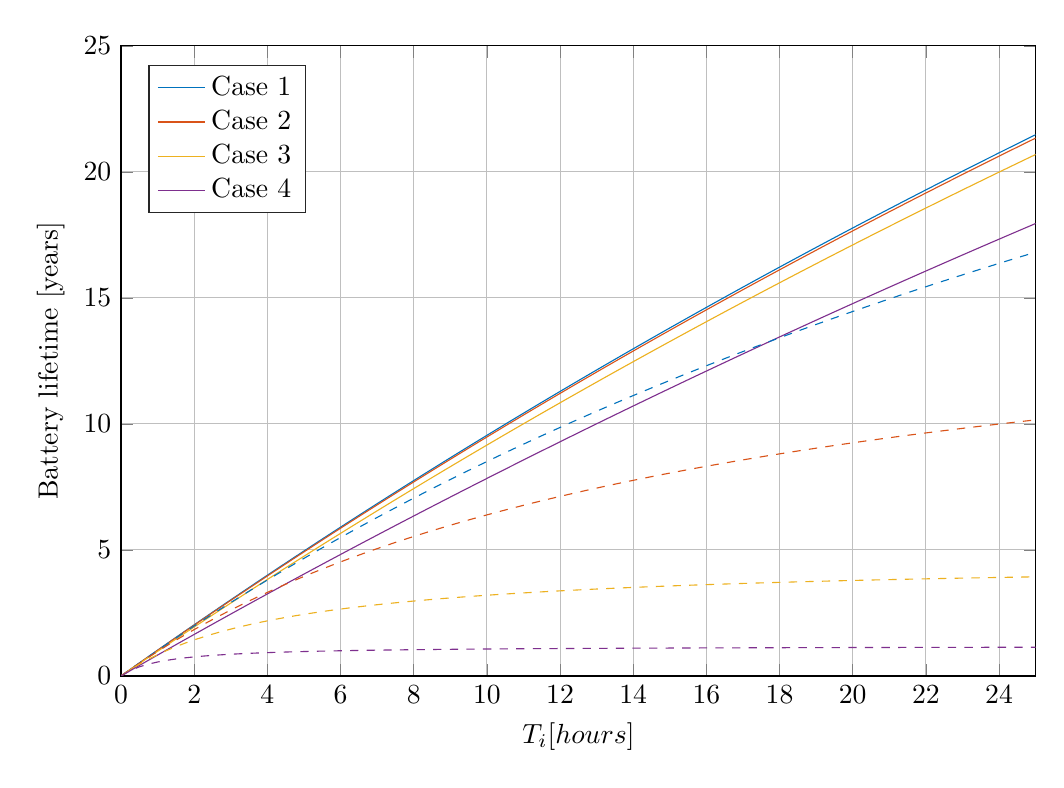
\begin{tikzpicture}

\begin{axis}[%
width=0.958\textwidth,
height=0.66\textwidth,
at={(0\textwidth,0\textwidth)},
scale only axis,
xmin=0,
xmax=25,
xlabel={$\text{T}_\text{i}\text{ [hours]}$},
xmajorgrids,
ymin=0,
ymax=25,
ylabel={Battery lifetime [years]},
ymajorgrids,
axis background/.style={fill=white},
legend style={at={(0.03,0.97)},anchor=north west,legend cell align=left,align=left,draw=white!15!black},
y tick label style={/pgf/number format/fixed}
]
\addplot [color=mycolor1,solid]
  table[row sep=crcr]{%
0.000277777777777778	0.000286422124447134\\
0.250275	0.257547380536414\\
0.500272222222222	0.513781423703253\\
0.750269444444444	0.768994688123711\\
1.00026666666667	1.02319326150087\\
1.25026388888889	1.2763831832262\\
1.50026111111111	1.52857044485786\\
1.75025833333333	1.7797609905933\\
2.00025555555556	2.02996071773633\\
2.25025277777778	2.27917547715863\\
2.50025	2.52741107375581\\
2.75024722222222	2.77467326689815\\
3.00024444444444	3.02096777087598\\
3.25024166666667	3.26630025533995\\
3.50023888888889	3.51067634573601\\
3.75023611111111	3.75410162373543\\
4.00023333333333	3.99658162765978\\
4.25023055555556	4.23812185290089\\
4.50022777777778	4.47872775233609\\
4.750225	4.71840473673848\\
5.00022222222222	4.95715817518256\\
5.25021944444444	5.19499339544515\\
5.50021666666667	5.4319156844017\\
5.75021388888889	5.66793028841802\\
6.00021111111111	5.90304241373755\\
6.25020833333333	6.13725722686416\\
6.50020555555556	6.37057985494063\\
6.75020277777778	6.60301538612274\\
7.0002	6.83456886994918\\
7.25019722222222	7.06524531770717\\
7.50019444444444	7.29504970279403\\
7.75019166666667	7.52398696107457\\
8.00018888888889	7.7520619912345\\
8.25018611111111	7.97927965512981\\
8.50018333333333	8.20564477813229\\
8.75018055555556	8.43116214947106\\
9.00017777777778	8.65583652257035\\
9.250175	8.87967261538351\\
9.50017222222222	9.10267511072322\\
9.75016944444445	9.32484865658805\\
10.0001666666667	9.54619786648541\\
10.2501638888889	9.7667273197509\\
10.5001611111111	9.98644156186408\\
10.7501583333333	10.2053451047608\\
11.0001555555556	10.423442427142\\
11.2501527777778	10.6407379747792\\
11.50015	10.8572361608168\\
11.7501472222222	11.0729413660702\\
12.0001444444444	11.2878579393221\\
12.2501416666667	11.5019901976142\\
12.5001388888889	11.7153424265364\\
12.7501361111111	11.9279188805129\\
13.0001333333333	12.1397237830846\\
13.2501305555556	12.3507613271893\\
13.5001277777778	12.561035675438\\
13.750125	12.7705509603885\\
14.0001222222222	12.9793112848169\\
14.2501194444444	13.1873207219843\\
14.5001166666667	13.3945833159026\\
14.7501138888889	13.6011030815962\\
15.0001111111111	13.8068840053613\\
15.2501083333333	14.0119300450223\\
15.5001055555556	14.2162451301859\\
15.7501027777778	14.4198331624917\\
16.0001	14.6226980158607\\
16.2500972222222	14.8248435367411\\
16.5000944444444	15.0262735443516\\
16.7500916666667	15.2269918309213\\
17.0000888888889	15.4270021619283\\
17.2500861111111	15.626308276335\\
17.5000833333333	15.8249138868208\\
17.7500805555556	16.0228226800132\\
18.0000777777778	16.2200383167152\\
18.250075	16.4165644321318\\
18.5000722222222	16.6124046360926\\
18.7500694444444	16.8075625132735\\
19.0000666666667	17.0020416234149\\
19.2500638888889	17.1958455015384\\
19.5000611111111	17.388977658161\\
19.7500583333333	17.5814415795069\\
20.0000555555556	17.7732407277173\\
20.2500527777778	17.9643785410583\\
20.50005	18.154858434126\\
20.7500472222222	18.3446837980497\\
21.0000444444444	18.5338580006939\\
21.2500416666667	18.7223843868565\\
21.5000388888889	18.9102662784667\\
21.7500361111111	19.0975069747798\\
22.0000333333333	19.2841097525701\\
22.2500305555556	19.4700778663226\\
22.5000277777778	19.6554145484218\\
22.750025	19.8401230093389\\
23.0000222222222	20.0242064378177\\
23.2500194444444	20.2076680010575\\
23.5000166666667	20.3905108448951\\
23.7500138888889	20.5727380939844\\
24.0000111111111	20.7543528519747\\
24.2500083333333	20.9353582016866\\
24.5000055555556	21.1157572052866\\
24.7500027777778	21.2955529044596\\
25	21.47474832058\\
};
\addlegendentry{Case 1};

\addplot [color=mycolor2,solid]
  table[row sep=crcr]{%
0.000277777777777778	0.000284261257224411\\
0.250275	0.255608210845614\\
0.500272222222222	0.509920635804854\\
0.750269444444444	0.763227535333012\\
1.00026666666667	1.01553486128132\\
1.25026388888889	1.26684851862034\\
1.50026111111111	1.51717436590066\\
1.75025833333333	1.76651821570809\\
2.00025555555556	2.01488583511361\\
2.25025277777778	2.26228294611801\\
2.50025	2.50871522609127\\
2.75024722222222	2.75418830820687\\
3.00024444444444	2.99870778187105\\
3.25024166666667	3.24227919314703\\
3.50023888888889	3.48490804517432\\
3.75023611111111	3.72659979858321\\
4.00023333333333	3.96735987190437\\
4.25023055555556	4.20719364197387\\
4.50022777777778	4.44610644433339\\
4.750225	4.6841035736259\\
5.00022222222222	4.9211902839868\\
5.25021944444444	5.15737178943059\\
5.50021666666667	5.39265326423302\\
5.75021388888889	5.62703984330906\\
6.00021111111111	5.86053662258638\\
6.25020833333333	6.09314865937471\\
6.50020555555556	6.32488097273095\\
6.75020277777778	6.55573854382016\\
7.0002	6.78572631627249\\
7.25019722222222	7.01484919653604\\
7.50019444444444	7.24311205422579\\
7.75019166666667	7.47051972246858\\
8.00018888888889	7.69707699824423\\
8.25018611111111	7.92278864272284\\
8.50018333333333	8.14765938159831\\
8.75018055555556	8.37169390541819\\
9.00017777777778	8.59489686990975\\
9.250175	8.81727289630254\\
9.50017222222222	9.03882657164731\\
9.75016944444445	9.2595624491314\\
10.0001666666667	9.4794850483907\\
10.2501638888889	9.69859885581803\\
10.5001611111111	9.91690832486834\\
10.7501583333333	10.1344178763603\\
11.0001555555556	10.3511318987749\\
11.2501527777778	10.5670547485504\\
11.50015	10.7821907503742\\
11.7501472222222	10.996544197472\\
12.0001444444444	11.2101193518928\\
12.2501416666667	11.4229204447918\\
12.5001388888889	11.6349516767097\\
12.7501361111111	11.846217217849\\
13.0001333333333	12.0567212083475\\
13.2501305555556	12.2664677585487\\
13.5001277777778	12.4754609492696\\
13.750125	12.6837048320646\\
14.0001222222222	12.8912034294883\\
14.2501194444444	13.0979607353539\\
14.5001166666667	13.3039807149894\\
14.7501138888889	13.5092673054916\\
15.0001111111111	13.7138244159763\\
15.2501083333333	13.9176559278268\\
15.5001055555556	14.1207656949394\\
15.7501027777778	14.3231575439661\\
16.0001	14.5248352745551\\
16.2500972222222	14.7258026595883\\
16.5000944444444	14.926063445417\\
16.7500916666667	15.1256213520944\\
17.0000888888889	15.3244800736059\\
17.2500861111111	15.5226432780974\\
17.5000833333333	15.7201146081004\\
17.7500805555556	15.9168976807554\\
18.0000777777778	16.1129960880327\\
18.250075	16.3084133969512\\
18.5000722222222	16.5031531497942\\
18.7500694444444	16.6972188643239\\
19.0000666666667	16.8906140339931\\
19.2500638888889	17.0833421281544\\
19.5000611111111	17.2754065922685\\
19.7500583333333	17.4668108481086\\
20.0000555555556	17.6575582939643\\
20.2500527777778	17.8476523048424\\
20.50005	18.037096232666\\
20.7500472222222	18.2258934064716\\
21.0000444444444	18.4140471326039\\
21.2500416666667	18.6015606949091\\
21.5000388888889	18.7884373549258\\
21.7500361111111	18.9746803520739\\
22.0000333333333	19.1602929038422\\
22.2500305555556	19.3452782059734\\
22.5000277777778	19.5296394326475\\
22.750025	19.7133797366635\\
23.0000222222222	19.896502249619\\
23.2500194444444	20.0790100820882\\
23.5000166666667	20.2609063237981\\
23.7500138888889	20.4421940438025\\
24.0000111111111	20.6228762906551\\
24.2500083333333	20.8029560925801\\
24.5000055555556	20.9824364576412\\
24.7500027777778	21.1613203739096\\
25	21.3396108096295\\
};
\addlegendentry{Case 2};

\addplot [color=mycolor3,solid]
  table[row sep=crcr]{%
0.000277777777777778	0.000273928212981524\\
0.250275	0.246334492348347\\
0.500272222222222	0.491455531003821\\
0.750269444444444	0.735642414967686\\
1.00026666666667	0.978900474170003\\
1.25026388888889	1.22123499807041\\
1.50026111111111	1.46265123604149\\
1.75025833333333	1.70315439774787\\
2.00025555555556	1.94274965352088\\
2.25025277777778	2.18144213472915\\
2.50025	2.41923693414488\\
2.75024722222222	2.65613910630608\\
3.00024444444444	2.89215366787467\\
3.25024166666667	3.12728559799066\\
3.50023888888889	3.3615398386222\\
3.75023611111111	3.59492129491193\\
4.00023333333333	3.82743483551927\\
4.25023055555556	4.059085292959\\
4.50022777777778	4.28987746393608\\
4.750225	4.51981610967674\\
5.00022222222222	4.74890595625584\\
5.25021944444444	4.97715169492074\\
5.50021666666667	5.20455798241148\\
5.75021388888889	5.43112944127747\\
6.00021111111111	5.65687066019075\\
6.25020833333333	5.88178619425575\\
6.50020555555556	6.10588056531566\\
6.75020277777778	6.32915826225547\\
7.0002	6.55162374130174\\
7.25019722222222	6.77328142631903\\
7.50019444444444	6.99413570910313\\
7.75019166666667	7.21419094967114\\
8.00018888888889	7.43345147654841\\
8.25018611111111	7.65192158705229\\
8.50018333333333	7.86960554757294\\
8.75018055555556	8.08650759385102\\
9.00017777777778	8.30263193125244\\
9.250175	8.51798273504014\\
9.50017222222222	8.73256415064297\\
9.75016944444445	8.94638029392167\\
10.0001666666667	9.15943525143208\\
10.2501638888889	9.37173308068539\\
10.5001611111111	9.58327781040583\\
10.7501583333333	9.79407344078545\\
11.0001555555556	10.0041239437363\\
11.2501527777778	10.2134332631398\\
11.50015	10.4220053150937\\
11.7501472222222	10.6298439881563\\
12.0001444444444	10.836953143588\\
12.2501416666667	11.0433366155906\\
12.5001388888889	11.2489982115437\\
12.7501361111111	11.453941712239\\
13.0001333333333	11.6581708721119\\
13.2501305555556	11.8616894194709\\
13.5001277777778	12.0645010567241\\
13.750125	12.2666094606042\\
14.0001222222222	12.4680182823904\\
14.2501194444444	12.6687311481284\\
14.5001166666667	12.8687516588479\\
14.7501138888889	13.0680833907781\\
15.0001111111111	13.2667298955605\\
15.2501083333333	13.4646947004605\\
15.5001055555556	13.6619813085754\\
15.7501027777778	13.8585931990415\\
16.0001	14.0545338272388\\
16.2500972222222	14.2498066249927\\
16.5000944444444	14.4444150007751\\
16.7500916666667	14.6383623399024\\
17.0000888888889	14.8316520047318\\
17.2500861111111	15.0242873348555\\
17.5000833333333	15.2162716472933\\
17.7500805555556	15.4076082366828\\
18.0000777777778	15.598300375468\\
18.250075	15.7883513140858\\
18.5000722222222	15.9777642811505\\
18.7500694444444	16.166542483637\\
19.0000666666667	16.3546891070615\\
19.2500638888889	16.5422073156608\\
19.5000611111111	16.7291002525696\\
19.7500583333333	16.9153710399963\\
20.0000555555556	17.1010227793967\\
20.2500527777778	17.2860585516462\\
20.50005	17.4704814172101\\
20.7500472222222	17.6542944163126\\
21.0000444444444	17.8375005691037\\
21.2500416666667	18.0201028758245\\
21.5000388888889	18.2021043169711\\
21.7500361111111	18.3835078534569\\
22.0000333333333	18.564316426773\\
22.2500305555556	18.744532959147\\
22.5000277777778	18.9241603537009\\
22.750025	19.1032014946068\\
23.0000222222222	19.2816592472408\\
23.2500194444444	19.4595364583367\\
23.5000166666667	19.6368359561368\\
23.7500138888889	19.8135605505418\\
24.0000111111111	19.9897130332596\\
24.2500083333333	20.1652961779519\\
24.5000055555556	20.3403127403801\\
24.7500027777778	20.5147654585491\\
25	20.6886570528507\\
};
\addlegendentry{Case 3};

\addplot [color=mycolor4,solid]
  table[row sep=crcr]{%
0.000277777777777778	0.000231798274947652\\
0.250275	0.20850978672527\\
0.500272222222222	0.416114428887904\\
0.750269444444444	0.623048984806173\\
1.00026666666667	0.829316693512402\\
1.25026388888889	1.03492077319692\\
1.50026111111111	1.23986442137541\\
1.75025833333333	1.4441508150547\\
2.00025555555556	1.6477831108969\\
2.25025277777778	1.85076444538202\\
2.50025	2.05309793496898\\
2.75024722222222	2.25478667625511\\
3.00024444444444	2.45583374613416\\
3.25024166666667	2.65624220195272\\
3.50023888888889	2.85601508166521\\
3.75023611111111	3.05515540398743\\
4.00023333333333	3.25366616854854\\
4.25023055555556	3.45155035604174\\
4.50022777777778	3.64881092837342\\
4.750225	3.84545082881094\\
5.00022222222222	4.04147298212904\\
5.25021944444444	4.23688029475482\\
5.50021666666667	4.4316756549114\\
5.75021388888889	4.62586193276025\\
6.00021111111111	4.8194419805421\\
6.25020833333333	5.01241863271662\\
6.50020555555556	5.20479470610076\\
6.75020277777778	5.39657300000583\\
7.0002	5.58775629637322\\
7.25019722222222	5.77834735990899\\
7.50019444444444	5.96834893821707\\
7.75019166666667	6.15776376193136\\
8.00018888888889	6.34659454484649\\
8.25018611111111	6.53484398404746\\
8.50018333333333	6.72251476003803\\
8.75018055555556	6.90960953686795\\
9.00017777777778	7.09613096225904\\
9.250175	7.28208166773006\\
9.50017222222222	7.46746426872048\\
9.75016944444445	7.65228136471313\\
10.0001666666667	7.83653553935564\\
10.2501638888889	8.02022936058089\\
10.5001611111111	8.2033653807263\\
10.7501583333333	8.38594613665201\\
11.0001555555556	8.56797414985807\\
11.2501527777778	8.74945192660046\\
11.50015	8.93038195800616\\
11.7501472222222	9.11076672018712\\
12.0001444444444	9.29060867435322\\
12.2501416666667	9.46991026692421\\
12.5001388888889	9.64867392964061\\
12.7501361111111	9.8269020796737\\
13.0001333333333	10.0045971197344\\
13.2501305555556	10.1817614381814\\
13.5001277777778	10.3583974091279\\
13.750125	10.5345073925478\\
14.0001222222222	10.710093734381\\
14.2501194444444	10.8851587666371\\
14.5001166666667	11.0597048074992\\
14.7501138888889	11.2337341614258\\
15.0001111111111	11.4072491192523\\
15.2501083333333	11.5802519582917\\
15.5001055555556	11.752744942434\\
15.7501027777778	11.9247303222452\\
16.0001	12.0962103350649\\
16.2500972222222	12.2671872051035\\
16.5000944444444	12.4376631435384\\
16.7500916666667	12.6076403486092\\
17.0000888888889	12.7771210057121\\
17.2500861111111	12.9461072874939\\
17.5000833333333	13.1146013539445\\
17.7500805555556	13.2826053524891\\
18.0000777777778	13.4501214180794\\
18.250075	13.6171516732841\\
18.5000722222222	13.7836982283783\\
18.7500694444444	13.9497631814327\\
19.0000666666667	14.1153486184015\\
19.2500638888889	14.2804566132098\\
19.5000611111111	14.4450892278402\\
19.7500583333333	14.6092485124186\\
20.0000555555556	14.7729365052992\\
20.2500527777778	14.9361552331493\\
20.50005	15.0989067110322\\
20.7500472222222	15.2611929424909\\
21.0000444444444	15.4230159196299\\
21.2500416666667	15.5843776231967\\
21.5000388888889	15.7452800226626\\
21.7500361111111	15.9057250763032\\
22.0000333333333	16.0657147312774\\
22.2500305555556	16.2252509237064\\
22.5000277777778	16.3843355787516\\
22.750025	16.5429706106923\\
23.0000222222222	16.7011579230025\\
23.2500194444444	16.8588994084266\\
23.5000166666667	17.0161969490553\\
23.7500138888889	17.1730524164006\\
24.0000111111111	17.3294676714693\\
24.2500083333333	17.4854445648375\\
24.5000055555556	17.6409849367229\\
24.7500027777778	17.7960906170574\\
25	17.950763425559\\
};
\addlegendentry{Case 4};

\addplot [color=mycolor1,dashed,forget plot]
  table[row sep=crcr]{%
0.000277777777777778	0.000286970534772933\\
0.250275	0.257178663126515\\
0.500272222222222	0.511344822105601\\
0.750269444444444	0.762828594065652\\
1.00026666666667	1.01167221967049\\
1.25026388888889	1.25791705730672\\
1.50026111111111	1.50160360599918\\
1.75025833333333	1.74277152761575\\
2.00025555555556	1.98145966838734\\
2.25025277777778	2.21770607976732\\
2.50025	2.45154803865413\\
2.75024722222222	2.68302206699954\\
3.00024444444444	2.91216395082418\\
3.25024166666667	3.13900875866129\\
3.50023888888889	3.36359085944847\\
3.75023611111111	3.58594393988675\\
4.00023333333333	3.80610102128533\\
4.25023055555556	4.02409447590964\\
4.50022777777778	4.23995604284985\\
4.750225	4.45371684342598\\
5.00022222222222	4.66540739614553\\
5.25021944444444	4.87505763122853\\
5.50021666666667	5.08269690471465\\
5.75021388888889	5.28835401216631\\
6.00021111111111	5.4920572019812\\
6.25020833333333	5.69383418832719\\
6.50020555555556	5.89371216371196\\
6.75020277777778	6.09171781119946\\
7.0002	6.28787731628463\\
7.25019722222222	6.48221637843758\\
7.50019444444444	6.6747602223277\\
7.75019166666667	6.86553360873835\\
8.00018888888889	7.05456084518164\\
8.25018611111111	7.24186579622325\\
8.50018333333333	7.42747189352618\\
8.75018055555556	7.61140214562249\\
9.00017777777778	7.79367914742157\\
9.250175	7.97432508946311\\
9.50017222222222	8.15336176692282\\
9.75016944444445	8.33081058837851\\
10.0001666666667	8.50669258434403\\
10.2501638888889	8.68102841557802\\
10.5001611111111	8.85383838117462\\
10.7501583333333	9.02514242644259\\
11.0001555555556	9.19496015057942\\
11.2501527777778	9.36331081414642\\
11.50015	9.53021334635101\\
11.7501472222222	9.69568635214191\\
12.0001444444444	9.85974811912268\\
12.2501416666667	10.0224166242893\\
12.5001388888889	10.1837095405965\\
12.7501361111111	10.3436442433587\\
13.0001333333333	10.5022378164897\\
13.2501305555556	10.6595070585854\\
13.5001277777778	10.8154684888563\\
13.750125	10.9701383529108\\
14.0001222222222	11.1235326283972\\
14.2501194444444	11.2756670305049\\
14.5001166666667	11.4265570173321\\
14.7501138888889	11.5762177951216\\
15.0001111111111	11.7246643233691\\
15.2501083333333	11.871911319808\\
15.5001055555556	12.0179732652735\\
15.7501027777778	12.1628644084503\\
16.0001	12.3065987705058\\
16.2500972222222	12.4491901496133\\
16.5000944444444	12.5906521253677\\
16.7500916666667	12.7309980630964\\
17.0000888888889	12.8702411180691\\
17.2500861111111	13.008394239608\\
17.5000833333333	13.1454701751023\\
17.7500805555556	13.2814814739294\\
18.0000777777778	13.4164404912846\\
18.250075	13.5503593919225\\
18.5000722222222	13.6832501538122\\
18.7500694444444	13.8151245717085\\
19.0000666666667	13.9459942606419\\
19.2500638888889	14.0758706593283\\
19.5000611111111	14.2047650335026\\
19.7500583333333	14.3326884791757\\
20.0000555555556	14.4596519258189\\
20.2500527777778	14.5856661394766\\
20.50005	14.7107417258098\\
20.7500472222222	14.8348891330716\\
21.0000444444444	14.958118655016\\
21.2500416666667	15.0804404337443\\
21.5000388888889	15.2018644624865\\
21.7500361111111	15.3224005883234\\
22.0000333333333	15.4420585148488\\
22.2500305555556	15.560847804773\\
22.5000277777778	15.6787778824707\\
22.750025	15.7958580364735\\
23.0000222222222	15.9120974219085\\
23.2500194444444	16.0275050628848\\
23.5000166666667	16.1420898548288\\
23.7500138888889	16.2558605667699\\
24.0000111111111	16.3688258435778\\
24.2500083333333	16.4809942081514\\
24.5000055555556	16.5923740635634\\
24.7500027777778	16.702973695158\\
25	16.8128012726056\\
};
\addplot [color=mycolor2,dashed,forget plot]
  table[row sep=crcr]{%
0.000277777777777778	0.000286978924939821\\
0.250275	0.254637555954174\\
0.500272222222222	0.501376617942425\\
0.750269444444444	0.74084079324313\\
1.00026666666667	0.973347148205504\\
1.25026388888889	1.19919458780003\\
1.50026111111111	1.41866513760232\\
1.75025833333333	1.63202511869683\\
2.00025555555556	1.83952622579177\\
2.25025277777778	2.04140651772178\\
2.50025	2.23789132853357\\
2.75024722222222	2.42919410648559\\
3.00024444444444	2.61551718752889\\
3.25024166666667	2.79705250916204\\
3.50023888888889	2.97398226995437\\
3.75023611111111	3.14647953950152\\
4.00023333333333	3.31470882310589\\
4.25023055555556	3.47882658505468\\
4.50022777777778	3.63898173399437\\
4.750225	3.79531607356669\\
5.00022222222222	3.94796472117222\\
5.25021944444444	4.09705649746131\\
5.50021666666667	4.24271428891177\\
5.75021388888889	4.38505538563849\\
6.00021111111111	4.52419179638654\\
6.25020833333333	4.6602305424857\\
6.50020555555556	4.79327393238781\\
6.75020277777778	4.92341981826694\\
7.0002	5.05076183603494\\
7.25019722222222	5.1753896300096\\
7.50019444444444	5.29738906336834\\
7.75019166666667	5.41684241542548\\
8.00018888888889	5.53382856668594\\
8.25018611111111	5.64842317254967\\
8.50018333333333	5.76069882647081\\
8.75018055555556	5.87072521331091\\
9.00017777777778	5.97856925356705\\
9.250175	6.08429523910189\\
9.50017222222222	6.1879649609545\\
9.75016944444445	6.28963782976544\\
10.0001666666667	6.38937098930956\\
10.2501638888889	6.48721942359226\\
10.5001611111111	6.58323605793095\\
10.7501583333333	6.6774718544122\\
11.0001555555556	6.76997590208631\\
11.2501527777778	6.86079550223467\\
11.50015	6.94997624902121\\
11.7501472222222	7.03756210581667\\
12.0001444444444	7.12359547746438\\
12.2501416666667	7.20811727873694\\
12.5001388888889	7.29116699921603\\
12.7501361111111	7.3727827648116\\
13.0001333333333	7.45300139612168\\
13.2501305555556	7.53185846382052\\
13.5001277777778	7.60938834125022\\
13.750125	7.68562425437898\\
14.0001222222222	7.7605983292788\\
14.2501194444444	7.83434163726487\\
14.5001166666667	7.90688423783021\\
14.7501138888889	7.97825521949985\\
15.0001111111111	8.04848273872153\\
15.2501083333333	8.11759405690196\\
15.5001055555556	8.18561557569097\\
15.7501027777778	8.25257287060968\\
16.0001	8.31849072311242\\
16.2500972222222	8.38339315116704\\
16.5000944444444	8.44730343843279\\
16.7500916666667	8.51024416211026\\
17.0000888888889	8.57223721953332\\
17.2500861111111	8.63330385356896\\
17.5000833333333	8.69346467688678\\
17.7500805555556	8.75273969515645\\
18.0000777777778	8.81114832922808\\
18.250075	8.86870943634694\\
18.5000722222222	8.92544133045142\\
18.7500694444444	8.98136180159998\\
19.0000666666667	9.03648813457048\\
19.2500638888889	9.09083712667268\\
19.5000611111111	9.14442510481253\\
19.7500583333333	9.19726794184453\\
20.0000555555556	9.24938107224675\\
20.2500527777778	9.30077950715092\\
20.50005	9.35147784875831\\
20.7500472222222	9.40149030417053\\
21.0000444444444	9.45083069866281\\
21.2500416666667	9.49951248842572\\
21.5000388888889	9.5475487728\\
21.7500361111111	9.594952306028\\
22.0000333333333	9.64173550854368\\
22.2500305555556	9.6879104778223\\
22.5000277777778	9.73348899880972\\
22.750025	9.77848255395004\\
23.0000222222222	9.82290233282972\\
23.2500194444444	9.86675924145496\\
23.5000166666667	9.91006391117875\\
23.7500138888889	9.95282670729273\\
24.0000111111111	9.9950577372985\\
24.2500083333333	10.0367668588724\\
24.5000055555556	10.0779636875365\\
24.7500027777778	10.1186576040493\\
25	10.1588577615264\\
};
\addplot [color=mycolor3,dashed,forget plot]
  table[row sep=crcr]{%
0.000277777777777778	0.000287012490514017\\
0.250275	0.244956193845469\\
0.500272222222222	0.465109095723427\\
0.750269444444444	0.664254772495307\\
1.00026666666667	0.845263098708633\\
1.25026388888889	1.01050396492601\\
1.50026111111111	1.16195161611871\\
1.75025833333333	1.30126390844605\\
2.00025555555556	1.42984324763776\\
2.25025277777778	1.54888396528675\\
2.50025	1.65940952845807\\
2.75024722222222	1.76230204005318\\
3.00024444444444	1.85832583117135\\
3.25024166666667	1.94814648126834\\
3.50023888888889	2.03234626754186\\
3.75023611111111	2.11143680190614\\
4.00023333333333	2.18586943526775\\
4.25023055555556	2.2560438761569\\
4.50022777777778	2.32231537131163\\
4.750225	2.38500072057431\\
5.00022222222222	2.44438334106015\\
5.25021944444444	2.50071755141757\\
5.50021666666667	2.55423221280197\\
5.75021388888889	2.60513383650017\\
6.00021111111111	2.65360924718253\\
6.25020833333333	2.69982787419008\\
6.50020555555556	2.74394373008728\\
6.75020277777778	2.78609712517137\\
7.0002	2.82641615815422\\
7.25019722222222	2.86501801638114\\
7.50019444444444	2.90201011338585\\
7.75019166666667	2.9374910870385\\
8.00018888888889	2.97155167781938\\
8.25018611111111	3.00427550368457\\
8.50018333333333	3.03573974545487\\
8.75018055555556	3.06601575455441\\
9.00017777777778	3.09516959317244\\
9.250175	3.12326251545512\\
9.50017222222222	3.15035139710405\\
9.75016944444445	3.17648911972184\\
10.0001666666667	3.20172491537022\\
10.2501638888889	3.22610467606443\\
10.5001611111111	3.24967123229728\\
10.7501583333333	3.27246460414945\\
11.0001555555556	3.29452222808292\\
11.2501527777778	3.31587916212116\\
11.50015	3.33656827178171\\
11.7501472222222	3.35662039883496\\
12.0001444444444	3.37606451471198\\
12.2501416666667	3.39492786016597\\
12.5001388888889	3.41323607260343\\
12.7501361111111	3.43101330233653\\
13.0001333333333	3.44828231886527\\
13.2501305555556	3.46506460817297\\
13.5001277777778	3.48138046190922\\
13.750125	3.49724905923877\\
14.0001222222222	3.51268854205027\\
14.2501194444444	3.52771608414523\\
14.5001166666667	3.54234795496169\\
14.7501138888889	3.55659957832984\\
15.0001111111111	3.5704855867057\\
15.2501083333333	3.58401987128355\\
15.5001055555556	3.59721562834823\\
15.7501027777778	3.61008540219202\\
16.0001	3.62264112488987\\
16.2500972222222	3.63489415319785\\
16.5000944444444	3.64685530281477\\
16.7500916666667	3.6585348802241\\
17.0000888888889	3.66994271231346\\
17.2500861111111	3.68108817395031\\
17.5000833333333	3.69198021367668\\
17.7500805555556	3.7026273776709\\
18.0000777777778	3.71303783211112\\
18.250075	3.7232193840637\\
18.5000722222222	3.7331795010087\\
18.7500694444444	3.7429253291051\\
19.0000666666667	3.75246371028969\\
19.2500638888889	3.76180119829556\\
19.5000611111111	3.77094407366897\\
19.7500583333333	3.77989835785706\\
20.0000555555556	3.78866982643254\\
20.2500527777778	3.79726402151673\\
20.50005	3.80568626345677\\
20.7500472222222	3.81394166180896\\
21.0000444444444	3.82203512567568\\
21.2500416666667	3.82997137344002\\
21.5000388888889	3.83775494193849\\
21.7500361111111	3.84539019510943\\
22.0000333333333	3.85288133215168\\
22.2500305555556	3.86023239522559\\
22.5000277777778	3.867447276726\\
22.750025	3.87452972615482\\
23.0000222222222	3.88148335661848\\
23.2500194444444	3.88831165097413\\
23.5000166666667	3.89501796764643\\
23.7500138888889	3.90160554613538\\
24.0000111111111	3.90807751223413\\
24.2500083333333	3.91443688297452\\
24.5000055555556	3.92068657131667\\
24.7500027777778	3.92682939059804\\
25	3.93286805875618\\
};
\addplot [color=mycolor4,dashed,forget plot]
  table[row sep=crcr]{%
0.000277777777777778	0.00028714683136536\\
0.250275	0.212620697168545\\
0.500272222222222	0.360733256010807\\
0.750269444444444	0.46993328851399\\
1.00026666666667	0.553775088560845\\
1.25026388888889	0.620172724636457\\
1.50026111111111	0.674057367246653\\
1.75025833333333	0.718661626831062\\
2.00025555555556	0.756192912698802\\
2.25025277777778	0.788209996604365\\
2.50025	0.81584495750367\\
2.75024722222222	0.839939831780708\\
3.00024444444444	0.861133909258571\\
3.25024166666667	0.879921290480437\\
3.50023888888889	0.896689889685017\\
3.75023611111111	0.91174850576027\\
4.00023333333333	0.925346013269348\\
4.25023055555556	0.937685225741433\\
4.50022777777778	0.948933080492118\\
4.750225	0.959228235463326\\
5.00022222222222	0.968686814123256\\
5.25021944444444	0.97740680456728\\
5.50021666666667	0.985471466809885\\
5.75021388888889	0.992951999698701\\
6.00021111111111	0.999909648582282\\
6.25020833333333	1.00639738592956\\
6.50020555555556	1.0124612625516\\
6.75020277777778	1.01814150236447\\
7.0002	1.02347339573975\\
7.25019722222222	1.02848803338797\\
7.50019444444444	1.03321291302528\\
7.75019166666667	1.03767244382909\\
8.00018888888889	1.04188836822448\\
8.25018611111111	1.04588011638686\\
8.50018333333333	1.04966510565848\\
8.75018055555556	1.05325899461325\\
9.00017777777778	1.05667589958671\\
9.250175	1.05992857998511\\
9.50017222222222	1.06302859750238\\
9.75016944444445	1.06598645343276\\
10.0001666666667	1.0688117075162\\
10.2501638888889	1.07151308115043\\
10.5001611111111	1.07409854731756\\
10.7501583333333	1.07657540917835\\
11.0001555555556	1.07895036896606\\
11.2501527777778	1.08122958854844\\
11.50015	1.08341874281023\\
11.7501472222222	1.08552306682993\\
12.0001444444444	1.08754739767649\\
12.2501416666667	1.08949621152833\\
12.5001388888889	1.09137365671431\\
12.7501361111111	1.09318358318992\\
13.0001333333333	1.09492956888952\\
13.2501305555556	1.09661494333409\\
13.5001277777778	1.09824280882238\\
13.750125	1.09981605948912\\
14.0001222222222	1.10133739847677\\
14.2501194444444	1.10280935343488\\
14.5001166666667	1.10423429053435\\
14.7501138888889	1.10561442715975\\
15.0001111111111	1.10695184342305\\
15.2501083333333	1.10824849262446\\
15.5001055555556	1.10950621077103\\
15.7501027777778	1.11072672525059\\
16.0001	1.1119116627471\\
16.2500972222222	1.11306255647386\\
16.5000944444444	1.11418085279206\\
16.7500916666667	1.11526791727477\\
17.0000888888889	1.11632504026995\\
17.2500861111111	1.11735344200992\\
17.5000833333333	1.11835427731005\\
17.7500805555556	1.11932863989453\\
18.0000777777778	1.12027756638341\\
18.250075	1.12120203997139\\
18.5000722222222	1.12210299382582\\
18.7500694444444	1.12298131422863\\
19.0000666666667	1.12383784348442\\
19.2500638888889	1.1246733826147\\
19.5000611111111	1.12548869385653\\
19.7500583333333	1.12628450298175\\
20.0000555555556	1.12706150145189\\
20.2500527777778	1.12782034842193\\
20.50005	1.12856167260531\\
20.7500472222222	1.12928607401124\\
21.0000444444444	1.12999412556431\\
21.2500416666667	1.13068637461571\\
21.5000388888889	1.13136334435439\\
21.7500361111111	1.13202553512575\\
22.0000333333333	1.13267342566493\\
22.2500305555556	1.13330747425106\\
22.5000277777778	1.13392811978831\\
22.750025	1.13453578281905\\
23.0000222222222	1.13513086647418\\
23.2500194444444	1.13571375736495\\
23.5000166666667	1.13628482642062\\
23.7500138888889	1.13684442967554\\
24.0000111111111	1.13739290900942\\
24.2500083333333	1.13793059284378\\
24.5000055555556	1.13845779679779\\
24.7500027777778	1.13897482430601\\
25	1.13948196720077\\
};
\end{axis}
\end{tikzpicture}%}
\caption{Battery life time estimation for the four cases for different $T_i$'s. Full line using PSM, dashed line using eDRX.}
\label{fig:eDRXvsPSM}
\end{figure}

As can be seen in \autoref{fig:eDRXvsPSM} the longer the $T_i$ the more impactful the these parameters become which makes sense as more time is spent in idle mode. What is also interesting to note is that each case is going asymptotic towards certain values and that eDRX is more influenced by the timer values than PSM is. To give a more clear picture of the influence of the timer values the $T_i$ is set to 24 hours and the timer values are changed are varied according to the values found in \autoref{sec:Network_access} this can be seen in \autoref{fig:TimerPlot_plots}.


\begin{figure}[H]
\centering
\begin{minipage}{0.48\textwidth}
\tikzsetnextfilename{eDRX_each_day_TimerPlot}
\resizebox{\textwidth}{!}{
% This file was created by matlab2tikz.
%
%The latest updates can be retrieved from
%  http://www.mathworks.com/matlabcentral/fileexchange/22022-matlab2tikz-matlab2tikz
%where you can also make suggestions and rate matlab2tikz.
%
\begin{tikzpicture}
\def\heightVar{0.66\textwidth};
\def\heightVarMid{0.33\textwidth};
\def\widthVar{\textwidth};
\def\widthVarMid{0.5\textwidth};

\begin{axis}[%
width=\textwidth,
height=0.66\textwidth,
at={(0\textwidth,0\textwidth)},
scale only axis,
point meta min=0.149128288181358,
point meta max=17.3415579519173,
xmin=2.56,
xmax=40.96,
xlabel={$\text{T}_{\text{PTW}}\text{ [s]}$},
xmajorgrids,
ymode=log,
ymin=20.48,
ymax=10485.76,
yminorticks=true,
ylabel={$\text{T}_{\text{PSM}}\text{ [s]}$},
ymajorgrids,
yminorgrids,
axis background/.style={fill=white},
title style={font=\bfseries},
title={eDRX with $T_{i} = 24 hours$},
%axis x line*=bottom,
%axis y line*=left,
y tick label style={/pgf/number format/fixed},
colormap={mymap}{[1pt] rgb(0pt)=(0.2081,0.1663,0.5292); rgb(1pt)=(0.211624,0.189781,0.577676); rgb(2pt)=(0.212252,0.213771,0.626971); rgb(3pt)=(0.2081,0.2386,0.677086); rgb(4pt)=(0.195905,0.264457,0.7279); rgb(5pt)=(0.170729,0.291938,0.779248); rgb(6pt)=(0.125271,0.324243,0.830271); rgb(7pt)=(0.0591333,0.359833,0.868333); rgb(8pt)=(0.0116952,0.38751,0.881957); rgb(9pt)=(0.00595714,0.408614,0.882843); rgb(10pt)=(0.0165143,0.4266,0.878633); rgb(11pt)=(0.0328524,0.443043,0.871957); rgb(12pt)=(0.0498143,0.458571,0.864057); rgb(13pt)=(0.0629333,0.47369,0.855438); rgb(14pt)=(0.0722667,0.488667,0.8467); rgb(15pt)=(0.0779429,0.503986,0.838371); rgb(16pt)=(0.0793476,0.520024,0.831181); rgb(17pt)=(0.0749429,0.537543,0.826271); rgb(18pt)=(0.0640571,0.556986,0.823957); rgb(19pt)=(0.0487714,0.577224,0.822829); rgb(20pt)=(0.0343429,0.596581,0.819852); rgb(21pt)=(0.0265,0.6137,0.8135); rgb(22pt)=(0.0238905,0.628662,0.803762); rgb(23pt)=(0.0230905,0.641786,0.791267); rgb(24pt)=(0.0227714,0.653486,0.776757); rgb(25pt)=(0.0266619,0.664195,0.760719); rgb(26pt)=(0.0383714,0.674271,0.743552); rgb(27pt)=(0.0589714,0.683757,0.725386); rgb(28pt)=(0.0843,0.692833,0.706167); rgb(29pt)=(0.113295,0.7015,0.685857); rgb(30pt)=(0.145271,0.709757,0.664629); rgb(31pt)=(0.180133,0.717657,0.642433); rgb(32pt)=(0.217829,0.725043,0.619262); rgb(33pt)=(0.258643,0.731714,0.595429); rgb(34pt)=(0.302171,0.737605,0.571186); rgb(35pt)=(0.348167,0.742433,0.547267); rgb(36pt)=(0.395257,0.7459,0.524443); rgb(37pt)=(0.44201,0.748081,0.503314); rgb(38pt)=(0.487124,0.749062,0.483976); rgb(39pt)=(0.530029,0.749114,0.466114); rgb(40pt)=(0.570857,0.748519,0.44939); rgb(41pt)=(0.609852,0.747314,0.433686); rgb(42pt)=(0.6473,0.7456,0.4188); rgb(43pt)=(0.683419,0.743476,0.404433); rgb(44pt)=(0.71841,0.741133,0.390476); rgb(45pt)=(0.752486,0.7384,0.376814); rgb(46pt)=(0.785843,0.735567,0.363271); rgb(47pt)=(0.818505,0.732733,0.34979); rgb(48pt)=(0.850657,0.7299,0.336029); rgb(49pt)=(0.882433,0.727433,0.3217); rgb(50pt)=(0.913933,0.725786,0.306276); rgb(51pt)=(0.944957,0.726114,0.288643); rgb(52pt)=(0.973895,0.731395,0.266648); rgb(53pt)=(0.993771,0.745457,0.240348); rgb(54pt)=(0.999043,0.765314,0.216414); rgb(55pt)=(0.995533,0.786057,0.196652); rgb(56pt)=(0.988,0.8066,0.179367); rgb(57pt)=(0.978857,0.827143,0.163314); rgb(58pt)=(0.9697,0.848138,0.147452); rgb(59pt)=(0.962586,0.870514,0.1309); rgb(60pt)=(0.958871,0.8949,0.113243); rgb(61pt)=(0.959824,0.921833,0.0948381); rgb(62pt)=(0.9661,0.951443,0.0755333); rgb(63pt)=(0.9763,0.9831,0.0538)},
colorbar,
colorbar style={ylabel={Battery Life Time [years]}}
]

\end{axis}


\node at (\widthVarMid, \heightVarMid) {
\includegraphics[width=\widthVar, height=\heightVar]{figures/QuectelMeas/eDRX_TimerPlot.png}};
\draw (0,0) -- (0,\heightVar) -- (\widthVar,\heightVar) -- (\widthVar,0) -- (0,0); 

\end{tikzpicture}}
\end{minipage}
\hfill
\begin{minipage}{0.48\textwidth}
\tikzsetnextfilename{PSM_each_day_TimerPlot}
\resizebox{\textwidth}{!}{
% This file was created by matlab2tikz.
%
%The latest updates can be retrieved from
%  http://www.mathworks.com/matlabcentral/fileexchange/22022-matlab2tikz-matlab2tikz
%where you can also make suggestions and rate matlab2tikz.
%
\definecolor{mycolor1}{rgb}{0.00000,0.44700,0.74100}%
%
\begin{tikzpicture}

\begin{axis}[%
width=\textwidth,
height=0.66\textwidth,
at={(0,0)},
scale only axis,
xmin=0,
xmax=100,
xlabel={$\text{T}_{\text{DRX}}\text{ [s]}$},
ymin=15.3,
ymax=16.3,
ylabel={Battery Life Time [years]},
axis background/.style={fill=white},
title style={font=\bfseries},
title={Scenario 4}
]
\addplot [color=mycolor1,solid,forget plot]
  table[row sep=crcr]{%
1	16.283020105401\\
2	16.2728459447618\\
3	16.2626844904762\\
4	16.2525357187561\\
5	16.2423996058724\\
6	16.2322761281554\\
7	16.2221652619942\\
8	16.2120669838368\\
9	16.2019812701897\\
10	16.191908097618\\
11	16.1818474427449\\
12	16.1717992822518\\
13	16.1617635928777\\
14	16.1517403514196\\
15	16.141729534732\\
16	16.1317311197265\\
17	16.1217450833722\\
18	16.1117714026949\\
19	16.1018100547774\\
20	16.091861016759\\
21	16.0819242658357\\
22	16.0719997792596\\
23	16.0620875343389\\
24	16.0521875084378\\
25	16.0422996789763\\
26	16.03242402343\\
27	16.0225605193299\\
28	16.0127091442623\\
29	16.0028698758685\\
30	15.9930426918448\\
31	15.9832275699422\\
32	15.9734244879664\\
33	15.9636334237774\\
34	15.9538543552895\\
35	15.944087260471\\
36	15.9343321173442\\
37	15.9245889039852\\
38	15.9148575985235\\
39	15.9051381791424\\
40	15.895430624078\\
41	15.8857349116198\\
42	15.8760510201101\\
43	15.8663789279442\\
44	15.8567186135696\\
45	15.8470700554868\\
46	15.8374332322481\\
47	15.8278081224582\\
48	15.8181947047737\\
49	15.8085929579031\\
50	15.7990028606065\\
51	15.7894243916956\\
52	15.7798575300332\\
53	15.7703022545336\\
54	15.7607585441619\\
55	15.7512263779344\\
56	15.7417057349177\\
57	15.7321965942294\\
58	15.7226989350372\\
59	15.7132127365593\\
60	15.703737978064\\
61	15.6942746388694\\
62	15.6848226983436\\
63	15.6753821359043\\
64	15.6659529310187\\
65	15.6565350632035\\
66	15.6471285120245\\
67	15.6377332570966\\
68	15.6283492780836\\
69	15.6189765546981\\
70	15.6096150667016\\
71	15.6002647939036\\
72	15.5909257161623\\
73	15.5815978133841\\
74	15.5722810655233\\
75	15.5629754525821\\
76	15.5536809546107\\
77	15.5443975517067\\
78	15.5351252240154\\
79	15.5258639517291\\
80	15.5166137150877\\
81	15.5073744943779\\
82	15.4981462699335\\
83	15.4889290221349\\
84	15.4797227314093\\
85	15.4705273782303\\
86	15.461342943118\\
87	15.4521694066387\\
88	15.4430067494045\\
89	15.433854952074\\
90	15.4247139953511\\
91	15.4155838599858\\
92	15.4064645267733\\
93	15.3973559765544\\
94	15.3882581902153\\
95	15.379171148687\\
96	15.3700948329459\\
97	15.3610292240131\\
98	15.3519743029543\\
99	15.3429300508802\\
100	15.3338964489456\\
};
\end{axis}
\end{tikzpicture}%}
\end{minipage}
\caption{Influence of timer settings for the estimated battery lifetime.}
\label{fig:TimerPlot_plots}
\end{figure}

From \autoref{fig:TimerPlot_plots} it can be seen that the values for the eDRX timers are very influential, as the expected lifetime is varying from 0.15 years to 17.34 years, where for PSM the lifetime only varies from 15.33 to 16.28 years. The next step is to look at the influence of $T_{transmit}$ and $P_{TX}$. To do this four scenarios are picked such that the differences for high and low $T_i$'s in each idle mode can be compared, the values chosen to showcase this can be seen in \autoref{tab:scenario_description}.


\begin{table}[H]
\centering
\begin{tabular}{|c|c|c|c|c|c|} \hline
			& $T_i$ 		& Idle mode	& $T_{DRX}$	& $T_{PSM}$	& $T_{PTW}$	\\ \hline
Scenario 1	& 1 hour 	& eDRX 		& -			& 10485.76 s& 10.24 s	\\ \hline
Scenario 2	& 24 hours 	& eDRX 		& -			& 10485.76 s& 10.24 s	\\ \hline
Scenario 3	& 1 hour 	& PSM		& 10 s		& -			& -			\\ \hline
Scenario 4	& 24 hours 	& PSM		& 10 s		& -			& -			\\ \hline
\end{tabular}
\caption{Parameter values chosen for each scenario.}
\label{tab:scenario_description}
\end{table}

For each of the four scenarios the transmit power and transmit time is varied independent of each other and the battery lifetime is estimated for each combination as seen in \autoref{fig:lifetime_plots}.


\begin{figure}[H]
\centering
\begin{minipage}{0.48\textwidth}
\tikzsetnextfilename{eDRX_each_hour_lifetime}
\resizebox{\textwidth}{!}{
% This file was created by matlab2tikz.
%
%The latest updates can be retrieved from
%  http://www.mathworks.com/matlabcentral/fileexchange/22022-matlab2tikz-matlab2tikz
%where you can also make suggestions and rate matlab2tikz.
%
\begin{tikzpicture}
\def\heightVar{0.66\textwidth};
\def\heightVarMid{0.33\textwidth};
\def\widthVar{\textwidth};
\def\widthVarMid{0.5\textwidth};

\begin{axis}[%
width=\textwidth,
height=0.66\textwidth,
at={(0,0)},
scale only axis,
point meta min=0.000324417682482898,
point meta max=4.05496621017927,
xmin=-30,
xmax=23,
xlabel={$\text{P}_{\text{TX}}\text{ [dBm]}$},
xmajorgrids,
ymode=log,
ymin=0.001,
ymax=1000,
yminorticks=true,
ylabel={$\text{T}_{\text{Transmit}}\text{ [s]}$},
ymajorgrids,
yminorgrids,
axis background/.style={fill=white},
title style={font=\bfseries},
title={Scenario 1},
%axis x line*=bottom,
%axis y line*=left,
y tick label style={/pgf/number format/fixed},
colormap={mymap}{[1pt] rgb(0pt)=(0.2081,0.1663,0.5292); rgb(1pt)=(0.211624,0.189781,0.577676); rgb(2pt)=(0.212252,0.213771,0.626971); rgb(3pt)=(0.2081,0.2386,0.677086); rgb(4pt)=(0.195905,0.264457,0.7279); rgb(5pt)=(0.170729,0.291938,0.779248); rgb(6pt)=(0.125271,0.324243,0.830271); rgb(7pt)=(0.0591333,0.359833,0.868333); rgb(8pt)=(0.0116952,0.38751,0.881957); rgb(9pt)=(0.00595714,0.408614,0.882843); rgb(10pt)=(0.0165143,0.4266,0.878633); rgb(11pt)=(0.0328524,0.443043,0.871957); rgb(12pt)=(0.0498143,0.458571,0.864057); rgb(13pt)=(0.0629333,0.47369,0.855438); rgb(14pt)=(0.0722667,0.488667,0.8467); rgb(15pt)=(0.0779429,0.503986,0.838371); rgb(16pt)=(0.0793476,0.520024,0.831181); rgb(17pt)=(0.0749429,0.537543,0.826271); rgb(18pt)=(0.0640571,0.556986,0.823957); rgb(19pt)=(0.0487714,0.577224,0.822829); rgb(20pt)=(0.0343429,0.596581,0.819852); rgb(21pt)=(0.0265,0.6137,0.8135); rgb(22pt)=(0.0238905,0.628662,0.803762); rgb(23pt)=(0.0230905,0.641786,0.791267); rgb(24pt)=(0.0227714,0.653486,0.776757); rgb(25pt)=(0.0266619,0.664195,0.760719); rgb(26pt)=(0.0383714,0.674271,0.743552); rgb(27pt)=(0.0589714,0.683757,0.725386); rgb(28pt)=(0.0843,0.692833,0.706167); rgb(29pt)=(0.113295,0.7015,0.685857); rgb(30pt)=(0.145271,0.709757,0.664629); rgb(31pt)=(0.180133,0.717657,0.642433); rgb(32pt)=(0.217829,0.725043,0.619262); rgb(33pt)=(0.258643,0.731714,0.595429); rgb(34pt)=(0.302171,0.737605,0.571186); rgb(35pt)=(0.348167,0.742433,0.547267); rgb(36pt)=(0.395257,0.7459,0.524443); rgb(37pt)=(0.44201,0.748081,0.503314); rgb(38pt)=(0.487124,0.749062,0.483976); rgb(39pt)=(0.530029,0.749114,0.466114); rgb(40pt)=(0.570857,0.748519,0.44939); rgb(41pt)=(0.609852,0.747314,0.433686); rgb(42pt)=(0.6473,0.7456,0.4188); rgb(43pt)=(0.683419,0.743476,0.404433); rgb(44pt)=(0.71841,0.741133,0.390476); rgb(45pt)=(0.752486,0.7384,0.376814); rgb(46pt)=(0.785843,0.735567,0.363271); rgb(47pt)=(0.818505,0.732733,0.34979); rgb(48pt)=(0.850657,0.7299,0.336029); rgb(49pt)=(0.882433,0.727433,0.3217); rgb(50pt)=(0.913933,0.725786,0.306276); rgb(51pt)=(0.944957,0.726114,0.288643); rgb(52pt)=(0.973895,0.731395,0.266648); rgb(53pt)=(0.993771,0.745457,0.240348); rgb(54pt)=(0.999043,0.765314,0.216414); rgb(55pt)=(0.995533,0.786057,0.196652); rgb(56pt)=(0.988,0.8066,0.179367); rgb(57pt)=(0.978857,0.827143,0.163314); rgb(58pt)=(0.9697,0.848138,0.147452); rgb(59pt)=(0.962586,0.870514,0.1309); rgb(60pt)=(0.958871,0.8949,0.113243); rgb(61pt)=(0.959824,0.921833,0.0948381); rgb(62pt)=(0.9661,0.951443,0.0755333); rgb(63pt)=(0.9763,0.9831,0.0538)},
colorbar,
colorbar style={ylabel={Battery Life Time [years]}}
]

\end{axis}

\node at (\widthVarMid, \heightVarMid) {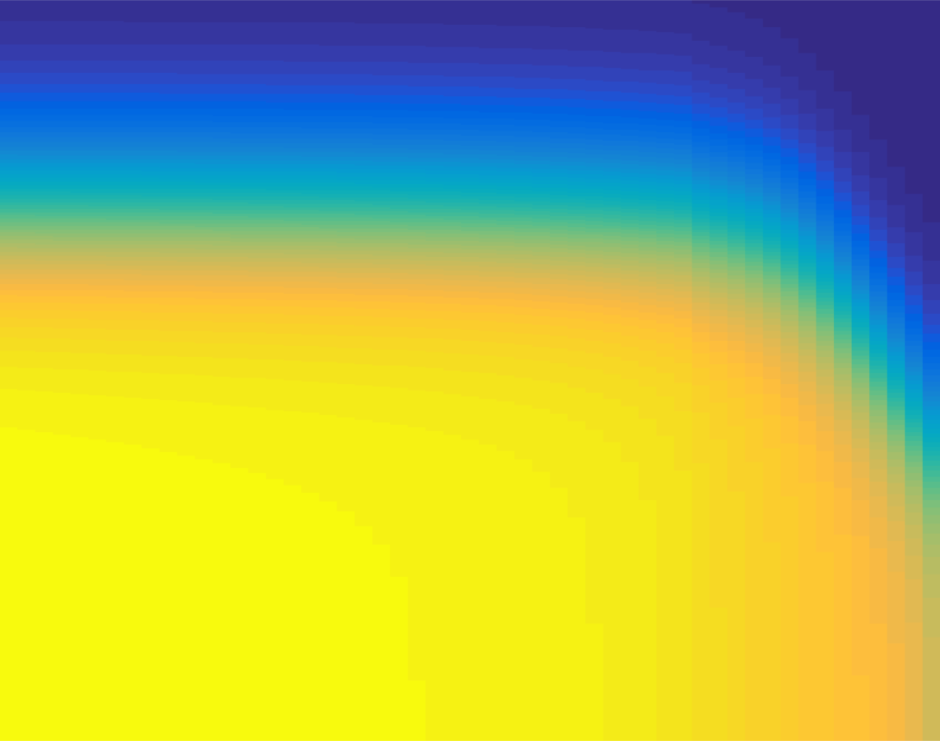
\includegraphics[width=\widthVar, height=\heightVar]{figures/QuectelMeas/eDRX_hour_lifetime.png}};
\draw (0,0) -- (0,\heightVar) -- (\widthVar,\heightVar) -- (\widthVar,0) -- (0,0); 

\end{tikzpicture}}
\end{minipage}
\hfill
\begin{minipage}{0.48\textwidth}
\tikzsetnextfilename{eDRX_each_day_lifetime}
\resizebox{\textwidth}{!}{
% This file was created by matlab2tikz.
%
%The latest updates can be retrieved from
%  http://www.mathworks.com/matlabcentral/fileexchange/22022-matlab2tikz-matlab2tikz
%where you can also make suggestions and rate matlab2tikz.
%
\begin{tikzpicture}
\def\heightVar{0.66\textwidth};
\def\heightVarMid{0.33\textwidth};
\def\widthVar{\textwidth};
\def\widthVarMid{0.5\textwidth};

\begin{axis}[%
width=\textwidth,
height=0.66\textwidth,
at={(0,0)},
scale only axis,
point meta min=0.00778467691738994,
point meta max=30.6920923323365,
xmin=-30,
xmax=23,
xlabel={$\text{P}_{\text{TX}}\text{ [dBm]}$},
xmajorgrids,
ymode=log,
ymin=0.001,
ymax=1000,
yminorticks=true,
ylabel={$\text{T}_{\text{Transmit}}\text{ [s]}$},
ymajorgrids,
yminorgrids,
axis background/.style={fill=white},
title style={font=\bfseries},
title={Scenario 2},
%axis x line*=bottom,
%axis y line*=left,
y tick label style={/pgf/number format/fixed},
colormap={mymap}{[1pt] rgb(0pt)=(0.2081,0.1663,0.5292); rgb(1pt)=(0.211624,0.189781,0.577676); rgb(2pt)=(0.212252,0.213771,0.626971); rgb(3pt)=(0.2081,0.2386,0.677086); rgb(4pt)=(0.195905,0.264457,0.7279); rgb(5pt)=(0.170729,0.291938,0.779248); rgb(6pt)=(0.125271,0.324243,0.830271); rgb(7pt)=(0.0591333,0.359833,0.868333); rgb(8pt)=(0.0116952,0.38751,0.881957); rgb(9pt)=(0.00595714,0.408614,0.882843); rgb(10pt)=(0.0165143,0.4266,0.878633); rgb(11pt)=(0.0328524,0.443043,0.871957); rgb(12pt)=(0.0498143,0.458571,0.864057); rgb(13pt)=(0.0629333,0.47369,0.855438); rgb(14pt)=(0.0722667,0.488667,0.8467); rgb(15pt)=(0.0779429,0.503986,0.838371); rgb(16pt)=(0.0793476,0.520024,0.831181); rgb(17pt)=(0.0749429,0.537543,0.826271); rgb(18pt)=(0.0640571,0.556986,0.823957); rgb(19pt)=(0.0487714,0.577224,0.822829); rgb(20pt)=(0.0343429,0.596581,0.819852); rgb(21pt)=(0.0265,0.6137,0.8135); rgb(22pt)=(0.0238905,0.628662,0.803762); rgb(23pt)=(0.0230905,0.641786,0.791267); rgb(24pt)=(0.0227714,0.653486,0.776757); rgb(25pt)=(0.0266619,0.664195,0.760719); rgb(26pt)=(0.0383714,0.674271,0.743552); rgb(27pt)=(0.0589714,0.683757,0.725386); rgb(28pt)=(0.0843,0.692833,0.706167); rgb(29pt)=(0.113295,0.7015,0.685857); rgb(30pt)=(0.145271,0.709757,0.664629); rgb(31pt)=(0.180133,0.717657,0.642433); rgb(32pt)=(0.217829,0.725043,0.619262); rgb(33pt)=(0.258643,0.731714,0.595429); rgb(34pt)=(0.302171,0.737605,0.571186); rgb(35pt)=(0.348167,0.742433,0.547267); rgb(36pt)=(0.395257,0.7459,0.524443); rgb(37pt)=(0.44201,0.748081,0.503314); rgb(38pt)=(0.487124,0.749062,0.483976); rgb(39pt)=(0.530029,0.749114,0.466114); rgb(40pt)=(0.570857,0.748519,0.44939); rgb(41pt)=(0.609852,0.747314,0.433686); rgb(42pt)=(0.6473,0.7456,0.4188); rgb(43pt)=(0.683419,0.743476,0.404433); rgb(44pt)=(0.71841,0.741133,0.390476); rgb(45pt)=(0.752486,0.7384,0.376814); rgb(46pt)=(0.785843,0.735567,0.363271); rgb(47pt)=(0.818505,0.732733,0.34979); rgb(48pt)=(0.850657,0.7299,0.336029); rgb(49pt)=(0.882433,0.727433,0.3217); rgb(50pt)=(0.913933,0.725786,0.306276); rgb(51pt)=(0.944957,0.726114,0.288643); rgb(52pt)=(0.973895,0.731395,0.266648); rgb(53pt)=(0.993771,0.745457,0.240348); rgb(54pt)=(0.999043,0.765314,0.216414); rgb(55pt)=(0.995533,0.786057,0.196652); rgb(56pt)=(0.988,0.8066,0.179367); rgb(57pt)=(0.978857,0.827143,0.163314); rgb(58pt)=(0.9697,0.848138,0.147452); rgb(59pt)=(0.962586,0.870514,0.1309); rgb(60pt)=(0.958871,0.8949,0.113243); rgb(61pt)=(0.959824,0.921833,0.0948381); rgb(62pt)=(0.9661,0.951443,0.0755333); rgb(63pt)=(0.9763,0.9831,0.0538)},
colorbar,
colorbar style={ylabel={Battery Life Time [years]}}
]

\end{axis}

\node at (\widthVarMid, \heightVarMid) {
\includegraphics[width=\widthVar, height=\heightVar]{figures/QuectelMeas/eDRX_day_lifetime.png}};
\draw (0,0) -- (0,\heightVar) -- (\widthVar,\heightVar) -- (\widthVar,0) -- (0,0); 

\end{tikzpicture}}
\end{minipage}
\begin{minipage}{0.48\textwidth}
\tikzsetnextfilename{PSM_each_hour_lifetime}
\resizebox{\textwidth}{!}{
% This file was created by matlab2tikz.
%
%The latest updates can be retrieved from
%  http://www.mathworks.com/matlabcentral/fileexchange/22022-matlab2tikz-matlab2tikz
%where you can also make suggestions and rate matlab2tikz.
%
\begin{tikzpicture}
\def\heightVar{0.66\textwidth};
\def\heightVarMid{0.33\textwidth};
\def\widthVar{\textwidth};
\def\widthVarMid{0.5\textwidth};

\begin{axis}[%
width=\textwidth,
height=0.66\textwidth,
at={(0,0)},
scale only axis,
point meta min=0.000324418159395187,
point meta max=4.10031859091161,
xmin=-30,
xmax=23,
xlabel={$\text{P}_{\text{TX}}\text{ [dBm]}$},
xmajorgrids,
ymode=log,
ymin=0.001,
ymax=1000,
yminorticks=true,
ylabel={$\text{T}_{\text{Transmit}}\text{ [s]}$},
ymajorgrids,
yminorgrids,
axis background/.style={fill=white},
title style={font=\bfseries},
title={Scenario 3},
%axis x line*=bottom,
%axis y line*=left,
y tick label style={/pgf/number format/fixed},
colormap={mymap}{[1pt] rgb(0pt)=(0.2081,0.1663,0.5292); rgb(1pt)=(0.211624,0.189781,0.577676); rgb(2pt)=(0.212252,0.213771,0.626971); rgb(3pt)=(0.2081,0.2386,0.677086); rgb(4pt)=(0.195905,0.264457,0.7279); rgb(5pt)=(0.170729,0.291938,0.779248); rgb(6pt)=(0.125271,0.324243,0.830271); rgb(7pt)=(0.0591333,0.359833,0.868333); rgb(8pt)=(0.0116952,0.38751,0.881957); rgb(9pt)=(0.00595714,0.408614,0.882843); rgb(10pt)=(0.0165143,0.4266,0.878633); rgb(11pt)=(0.0328524,0.443043,0.871957); rgb(12pt)=(0.0498143,0.458571,0.864057); rgb(13pt)=(0.0629333,0.47369,0.855438); rgb(14pt)=(0.0722667,0.488667,0.8467); rgb(15pt)=(0.0779429,0.503986,0.838371); rgb(16pt)=(0.0793476,0.520024,0.831181); rgb(17pt)=(0.0749429,0.537543,0.826271); rgb(18pt)=(0.0640571,0.556986,0.823957); rgb(19pt)=(0.0487714,0.577224,0.822829); rgb(20pt)=(0.0343429,0.596581,0.819852); rgb(21pt)=(0.0265,0.6137,0.8135); rgb(22pt)=(0.0238905,0.628662,0.803762); rgb(23pt)=(0.0230905,0.641786,0.791267); rgb(24pt)=(0.0227714,0.653486,0.776757); rgb(25pt)=(0.0266619,0.664195,0.760719); rgb(26pt)=(0.0383714,0.674271,0.743552); rgb(27pt)=(0.0589714,0.683757,0.725386); rgb(28pt)=(0.0843,0.692833,0.706167); rgb(29pt)=(0.113295,0.7015,0.685857); rgb(30pt)=(0.145271,0.709757,0.664629); rgb(31pt)=(0.180133,0.717657,0.642433); rgb(32pt)=(0.217829,0.725043,0.619262); rgb(33pt)=(0.258643,0.731714,0.595429); rgb(34pt)=(0.302171,0.737605,0.571186); rgb(35pt)=(0.348167,0.742433,0.547267); rgb(36pt)=(0.395257,0.7459,0.524443); rgb(37pt)=(0.44201,0.748081,0.503314); rgb(38pt)=(0.487124,0.749062,0.483976); rgb(39pt)=(0.530029,0.749114,0.466114); rgb(40pt)=(0.570857,0.748519,0.44939); rgb(41pt)=(0.609852,0.747314,0.433686); rgb(42pt)=(0.6473,0.7456,0.4188); rgb(43pt)=(0.683419,0.743476,0.404433); rgb(44pt)=(0.71841,0.741133,0.390476); rgb(45pt)=(0.752486,0.7384,0.376814); rgb(46pt)=(0.785843,0.735567,0.363271); rgb(47pt)=(0.818505,0.732733,0.34979); rgb(48pt)=(0.850657,0.7299,0.336029); rgb(49pt)=(0.882433,0.727433,0.3217); rgb(50pt)=(0.913933,0.725786,0.306276); rgb(51pt)=(0.944957,0.726114,0.288643); rgb(52pt)=(0.973895,0.731395,0.266648); rgb(53pt)=(0.993771,0.745457,0.240348); rgb(54pt)=(0.999043,0.765314,0.216414); rgb(55pt)=(0.995533,0.786057,0.196652); rgb(56pt)=(0.988,0.8066,0.179367); rgb(57pt)=(0.978857,0.827143,0.163314); rgb(58pt)=(0.9697,0.848138,0.147452); rgb(59pt)=(0.962586,0.870514,0.1309); rgb(60pt)=(0.958871,0.8949,0.113243); rgb(61pt)=(0.959824,0.921833,0.0948381); rgb(62pt)=(0.9661,0.951443,0.0755333); rgb(63pt)=(0.9763,0.9831,0.0538)},
colorbar,
colorbar style={ylabel={Battery Life Time [years]}}
]

\end{axis}

\node at (\widthVarMid, \heightVarMid) {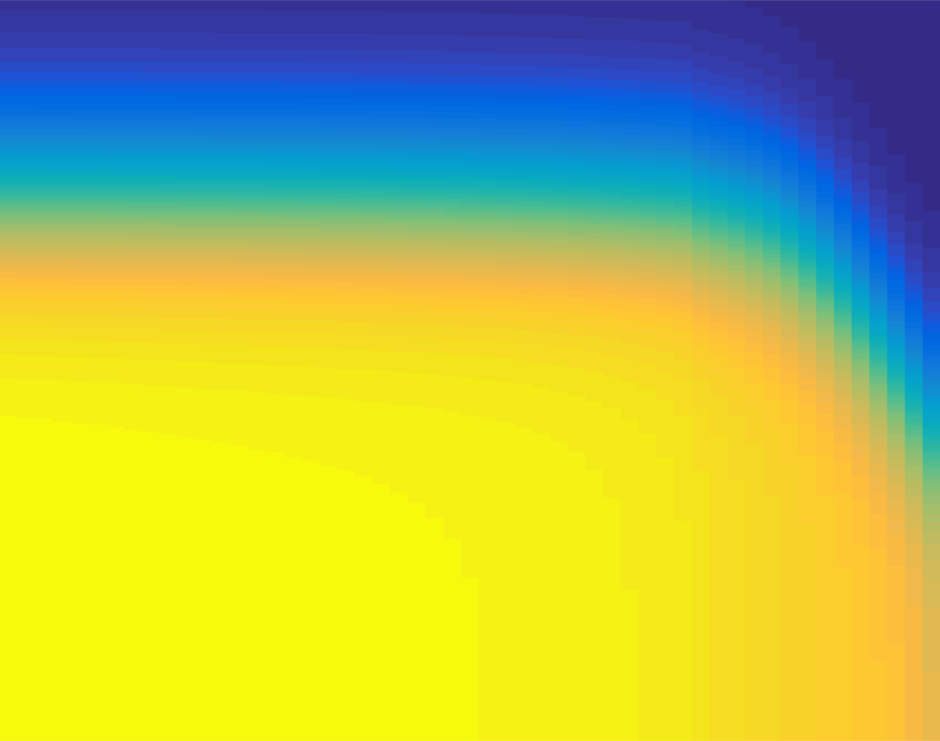
\includegraphics[width=\widthVar, height=\heightVar]{figures/QuectelMeas/PSM_hour_lifetime.png}};
\draw (0,0) -- (0,\heightVar) -- (\widthVar,\heightVar) -- (\widthVar,0) -- (0,0); 

\end{tikzpicture}}
\end{minipage}
\hfill
\begin{minipage}{0.48\textwidth}
\tikzsetnextfilename{PSM_each_day_lifetime}
\resizebox{\textwidth}{!}{
% This file was created by matlab2tikz.
%
%The latest updates can be retrieved from
%  http://www.mathworks.com/matlabcentral/fileexchange/22022-matlab2tikz-matlab2tikz
%where you can also make suggestions and rate matlab2tikz.
%
\begin{tikzpicture}
\def\heightVar{0.66\textwidth};
\def\heightVarMid{0.33\textwidth};
\def\widthVar{\textwidth};
\def\widthVarMid{0.5\textwidth};

\begin{axis}[%
width=\textwidth,
height=0.66\textwidth,
at={(0,0)},
scale only axis,
point meta min=0.00778520706091635,
point meta max=41.956503209313,
xmin=-30,
xmax=23,
xlabel={$\text{P}_{\text{TX}}\text{ [dBm]}$},
xmajorgrids,
ymode=log,
ymin=0.001,
ymax=1000,
yminorticks=true,
ylabel={$\text{T}_{\text{Transmit}}\text{ [s]}$},
ymajorgrids,
yminorgrids,
axis background/.style={fill=white},
title style={font=\bfseries},
title={Scenario 4},
%axis x line*=bottom,
%axis y line*=left,
y tick label style={/pgf/number format/fixed},
colormap={mymap}{[1pt] rgb(0pt)=(0.2081,0.1663,0.5292); rgb(1pt)=(0.211624,0.189781,0.577676); rgb(2pt)=(0.212252,0.213771,0.626971); rgb(3pt)=(0.2081,0.2386,0.677086); rgb(4pt)=(0.195905,0.264457,0.7279); rgb(5pt)=(0.170729,0.291938,0.779248); rgb(6pt)=(0.125271,0.324243,0.830271); rgb(7pt)=(0.0591333,0.359833,0.868333); rgb(8pt)=(0.0116952,0.38751,0.881957); rgb(9pt)=(0.00595714,0.408614,0.882843); rgb(10pt)=(0.0165143,0.4266,0.878633); rgb(11pt)=(0.0328524,0.443043,0.871957); rgb(12pt)=(0.0498143,0.458571,0.864057); rgb(13pt)=(0.0629333,0.47369,0.855438); rgb(14pt)=(0.0722667,0.488667,0.8467); rgb(15pt)=(0.0779429,0.503986,0.838371); rgb(16pt)=(0.0793476,0.520024,0.831181); rgb(17pt)=(0.0749429,0.537543,0.826271); rgb(18pt)=(0.0640571,0.556986,0.823957); rgb(19pt)=(0.0487714,0.577224,0.822829); rgb(20pt)=(0.0343429,0.596581,0.819852); rgb(21pt)=(0.0265,0.6137,0.8135); rgb(22pt)=(0.0238905,0.628662,0.803762); rgb(23pt)=(0.0230905,0.641786,0.791267); rgb(24pt)=(0.0227714,0.653486,0.776757); rgb(25pt)=(0.0266619,0.664195,0.760719); rgb(26pt)=(0.0383714,0.674271,0.743552); rgb(27pt)=(0.0589714,0.683757,0.725386); rgb(28pt)=(0.0843,0.692833,0.706167); rgb(29pt)=(0.113295,0.7015,0.685857); rgb(30pt)=(0.145271,0.709757,0.664629); rgb(31pt)=(0.180133,0.717657,0.642433); rgb(32pt)=(0.217829,0.725043,0.619262); rgb(33pt)=(0.258643,0.731714,0.595429); rgb(34pt)=(0.302171,0.737605,0.571186); rgb(35pt)=(0.348167,0.742433,0.547267); rgb(36pt)=(0.395257,0.7459,0.524443); rgb(37pt)=(0.44201,0.748081,0.503314); rgb(38pt)=(0.487124,0.749062,0.483976); rgb(39pt)=(0.530029,0.749114,0.466114); rgb(40pt)=(0.570857,0.748519,0.44939); rgb(41pt)=(0.609852,0.747314,0.433686); rgb(42pt)=(0.6473,0.7456,0.4188); rgb(43pt)=(0.683419,0.743476,0.404433); rgb(44pt)=(0.71841,0.741133,0.390476); rgb(45pt)=(0.752486,0.7384,0.376814); rgb(46pt)=(0.785843,0.735567,0.363271); rgb(47pt)=(0.818505,0.732733,0.34979); rgb(48pt)=(0.850657,0.7299,0.336029); rgb(49pt)=(0.882433,0.727433,0.3217); rgb(50pt)=(0.913933,0.725786,0.306276); rgb(51pt)=(0.944957,0.726114,0.288643); rgb(52pt)=(0.973895,0.731395,0.266648); rgb(53pt)=(0.993771,0.745457,0.240348); rgb(54pt)=(0.999043,0.765314,0.216414); rgb(55pt)=(0.995533,0.786057,0.196652); rgb(56pt)=(0.988,0.8066,0.179367); rgb(57pt)=(0.978857,0.827143,0.163314); rgb(58pt)=(0.9697,0.848138,0.147452); rgb(59pt)=(0.962586,0.870514,0.1309); rgb(60pt)=(0.958871,0.8949,0.113243); rgb(61pt)=(0.959824,0.921833,0.0948381); rgb(62pt)=(0.9661,0.951443,0.0755333); rgb(63pt)=(0.9763,0.9831,0.0538)},
colorbar,
colorbar style={ylabel={Battery Life Time [years]}}
]

\end{axis}

\node at (\widthVarMid, \heightVarMid) {
\includegraphics[width=\widthVar, height=\heightVar]{figures/QuectelMeas/PSM_day_lifetime.png}};
\draw (0,0) -- (0,\heightVar) -- (\widthVar,\heightVar) -- (\widthVar,0) -- (0,0); 

\end{tikzpicture}
}
\end{minipage}
\caption{The estimated battery lifetime for the mentioned scenarios with respect to transmit power and transmit duration.}
\label{fig:lifetime_plots}
\end{figure}

Here it can be seen again that the values of these parameters have a huge effect. Especially $T_{transmit}$ which alone can bring the lifetime down to less than a year no matter the other parameters. A realistic value for $T_{transmit}$ is not really known as it depends heavily on the usages as well as a multitude of cell parameters. To clarify the utilization of the energy spent four points has been picked out from each plot in \autoref{fig:lifetime_plots}. The values of each point can be seen in \autoref{tab:point_description}.

\begin{table}[H]
\centering
\begin{tabular}{|c|c|c|} \hline
& $T_{Transmit}$ & $P_{TX}$ \\ \hline
Point 1 & 100 ms& -20 dBm  	\\ \hline
Point 2 & 100 s	& -20 dBm  	\\ \hline
Point 3 & 100 ms& 23 dBm 	\\ \hline
Point 4 & 100 s	& 23 dBm 	\\ \hline
\end{tabular}
\caption{Points chosen to investigate.}
\label{tab:point_description}
\end{table} 

For each of the points in each of plots the energy usages has been divided up into five parts corresponding to the five elements in the model:  sync, attach, transmit, release and idle. The result of which can be seen in \autoref{fig:barplot_plots}.
 
\definecolor{mycolor1}{rgb}{0.00000,0.44700,0.74100}%
\definecolor{mycolor2}{rgb}{0.85000,0.32500,0.09800}%
\definecolor{mycolor3}{rgb}{0.92900,0.69400,0.12500}%
\definecolor{mycolor4}{rgb}{0.49400,0.18400,0.55600}%
\definecolor{mycolor5}{rgb}{0.46600,0.67400,0.18800}%
\begin{figure}[H]
\centering
\begin{minipage}{0.48\textwidth}
\tikzsetnextfilename{PSM_each_hour_barplot}
\resizebox{\textwidth}{!}{
% This file was created by matlab2tikz.
%
%The latest updates can be retrieved from
%  http://www.mathworks.com/matlabcentral/fileexchange/22022-matlab2tikz-matlab2tikz
%where you can also make suggestions and rate matlab2tikz.
%
\definecolor{mycolor1}{rgb}{0.00000,0.44700,0.74100}%
\definecolor{mycolor2}{rgb}{0.85000,0.32500,0.09800}%
\definecolor{mycolor3}{rgb}{0.92900,0.69400,0.12500}%
\definecolor{mycolor4}{rgb}{0.49400,0.18400,0.55600}%
\definecolor{mycolor5}{rgb}{0.46600,0.67400,0.18800}%
%
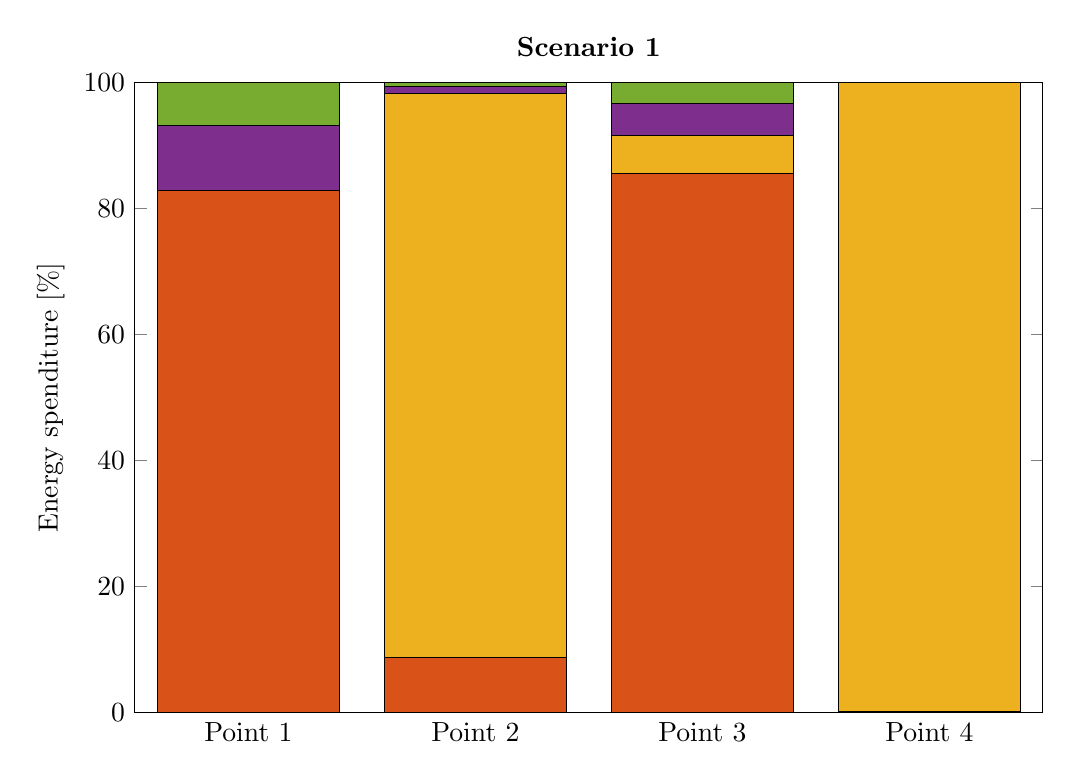
\begin{tikzpicture}

\begin{axis}[%
width=0.951\textwidth,
height=0.66\textwidth,
at={(0\textwidth,0\textwidth)},
scale only axis,
bar width=0.8,
xmin=0.5,
xmax=4.5,
xtick={1,2,3,4},
xticklabels={{Point 1},{Point 2},{Point 3},{Point 4}},
ymin=0,
ymax=100,
ylabel={Energy spenditure [\%]},
axis background/.style={fill=white},
title style={font=\bfseries},
title={Scenario 1},
y tick label style={/pgf/number format/fixed}
]
\addplot[ybar stacked,draw=black,fill=mycolor1,area legend] plot table[row sep=crcr] {%
1	0.000343025339696466\\
2	3.60428003392982e-05\\
3	0.000168149274421848\\
4	2.77486824917949e-07\\
};
\addplot[ybar stacked,draw=black,fill=mycolor2,area legend] plot table[row sep=crcr] {%
1	82.8187747118527\\
2	8.70204097436648\\
3	85.569279716967\\
4	0.141209932786317\\
};
\addplot[ybar stacked,draw=black,fill=mycolor3,area legend] plot table[row sep=crcr] {%
1	0.0851888329130451\\
2	89.5107078252492\\
3	6.05033028624487\\
4	99.8450303522011\\
};
\addplot[ybar stacked,draw=black,fill=mycolor4,area legend] plot table[row sep=crcr] {%
1	10.2942059241295\\
2	1.08164606469987\\
3	5.04616731353766\\
4	0.00832739213804403\\
};
\addplot[ybar stacked,draw=black,fill=mycolor5,area legend] plot table[row sep=crcr] 
\end{minipage}
\begin{minipage}{0.48\textwidth}
%Scenario 1
\begin{table}[H]
\centering
\resizebox{\textwidth}{!}{
\begin{tabular}{|c|c|c|c|c|} \hline
 & Pont 1	& Pont 2	& Pont 3	& Pont 4	\\ \hline
\cellcolor{mycolor5}Idle	& 4.6009\% 	& 0.8012\%	& 2.9499\%	& 0.0067\%\\ \hline
\cellcolor{mycolor4}Release	& 50.7850\% 	& 9.0970\%	& 32.5614\%	& 0.0763\%\\ \hline
\cellcolor{mycolor3}Transmit	& 0.0458\% 	& 82.1184\%	& 4.2587\%	& 99.7759\%\\ \hline
\cellcolor{mycolor2}Attach	& 44.5683\% 	& 7.9834\%	& 60.2301\%	& 0.1411\%\\ \hline
Lifetime (years)	& 2.1552 	& 0.3860	& 1.3818	& 0.0032\\ \hline
\end{tabular}}
\end{table}
\end{minipage}
\begin{minipage}{0.48\textwidth}
\tikzsetnextfilename{PSM_each_day_barplot}
\resizebox{\textwidth}{!}{
% This file was created by matlab2tikz.
%
%The latest updates can be retrieved from
%  http://www.mathworks.com/matlabcentral/fileexchange/22022-matlab2tikz-matlab2tikz
%where you can also make suggestions and rate matlab2tikz.
%
\definecolor{mycolor1}{rgb}{0.00000,0.44700,0.74100}%
\definecolor{mycolor2}{rgb}{0.85000,0.32500,0.09800}%
\definecolor{mycolor3}{rgb}{0.92900,0.69400,0.12500}%
\definecolor{mycolor4}{rgb}{0.49400,0.18400,0.55600}%
\definecolor{mycolor5}{rgb}{0.46600,0.67400,0.18800}%
%
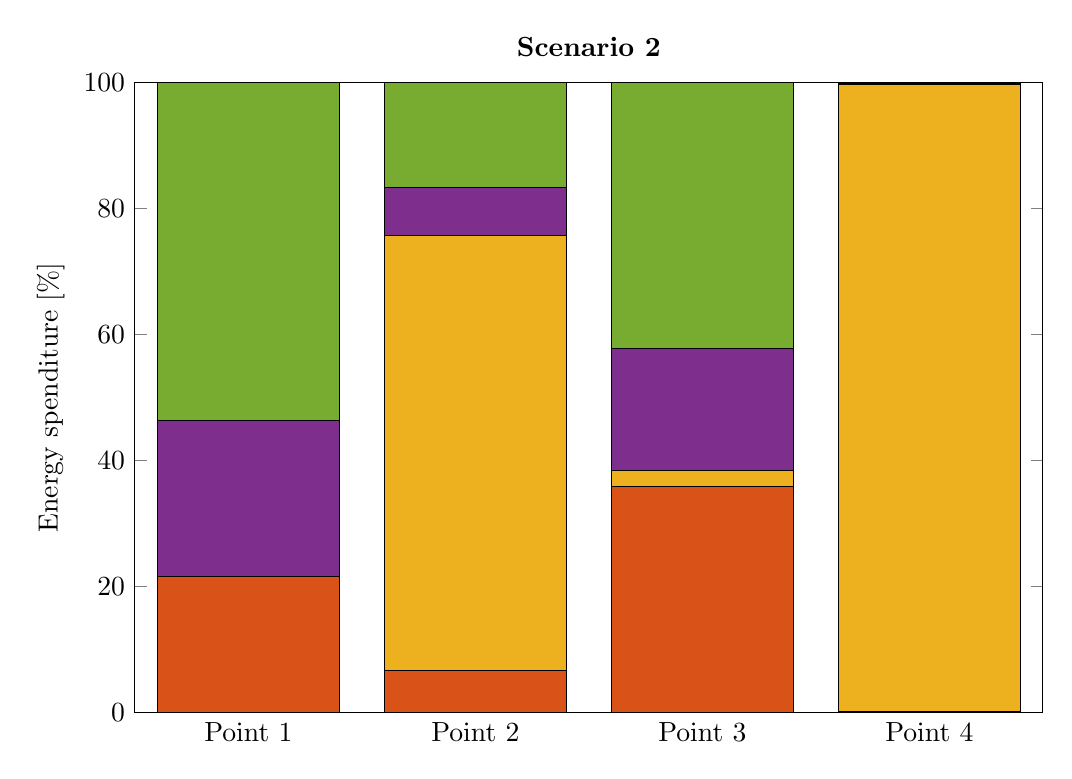
\begin{tikzpicture}

\begin{axis}[%
width=0.951\textwidth,
height=0.66\textwidth,
at={(0\textwidth,0\textwidth)},
scale only axis,
bar width=0.8,
xmin=0.5,
xmax=4.5,
xtick={1,2,3,4},
xticklabels={{Point 1},{Point 2},{Point 3},{Point 4}},
ymin=0,
ymax=100,
ylabel={Energy spenditure [\%]},
axis background/.style={fill=white},
title style={font=\bfseries},
title={Scenario 2},
y tick label style={/pgf/number format/fixed}
]
\addplot[ybar stacked,draw=black,fill=mycolor2,area legend] plot table[row sep=crcr] {%
1	21.6458916810439\\
2	6.71046797067417\\
3	35.8731879704054\\
4	0.140888017705163\\
};
\addplot[ybar stacked,draw=black,fill=mycolor3,area legend] plot table[row sep=crcr] {%
1	0.0222653408733227\\
2	69.025041328013\\
3	2.53647846936899\\
4	99.6174144868408\\
};
\addplot[ybar stacked,draw=black,fill=mycolor4,area legend] plot table[row sep=crcr] {%
1	24.6652203883008\\
2	7.64649356303764\\
3	19.3936347377525\\
4	0.076166376864918\\
};
\addplot[ybar stacked,draw=black,fill=mycolor5,area legend] plot table[row sep=crcr] 
\end{minipage}
\hfill
\begin{minipage}{0.48\textwidth}
%Scenario 2
\begin{table}[H]
\centering
\resizebox{\textwidth}{!}{
\begin{tabular}{|c|c|c|c|c|} \hline
 & Pont 1	& Pont 2	& Pont 3	& Pont 4	\\ \hline
\cellcolor{mycolor5}Idle	& 53.6666\% 	& 16.6180\%	& 42.1967\%	& 0.1655\%\\ \hline
\cellcolor{mycolor4}Release	& 24.6652\% 	& 7.6465\%	& 19.3936\%	& 0.0762\%\\ \hline
\cellcolor{mycolor3}Transmit	& 0.0223\% 	& 69.0250\%	& 2.5365\%	& 99.6174\%\\ \hline
\cellcolor{mycolor2}Attach	& 21.6459\% 	& 6.7105\%	& 35.8732\%	& 0.1409\%\\ \hline
Lifetime (years)	& 25.1212 	& 7.7878	& 19.7521	& 0.0776\\ \hline
\end{tabular}}
\end{table}
\end{minipage}
\hfill
\begin{minipage}{0.48\textwidth}
\tikzsetnextfilename{eDRX_each_hour_barplot}
\resizebox{\textwidth}{!}{
% This file was created by matlab2tikz.
%
%The latest updates can be retrieved from
%  http://www.mathworks.com/matlabcentral/fileexchange/22022-matlab2tikz-matlab2tikz
%where you can also make suggestions and rate matlab2tikz.
%
\definecolor{mycolor1}{rgb}{0.00000,0.44700,0.74100}%
\definecolor{mycolor2}{rgb}{0.85000,0.32500,0.09800}%
\definecolor{mycolor3}{rgb}{0.92900,0.69400,0.12500}%
\definecolor{mycolor4}{rgb}{0.49400,0.18400,0.55600}%
\definecolor{mycolor5}{rgb}{0.46600,0.67400,0.18800}%
%
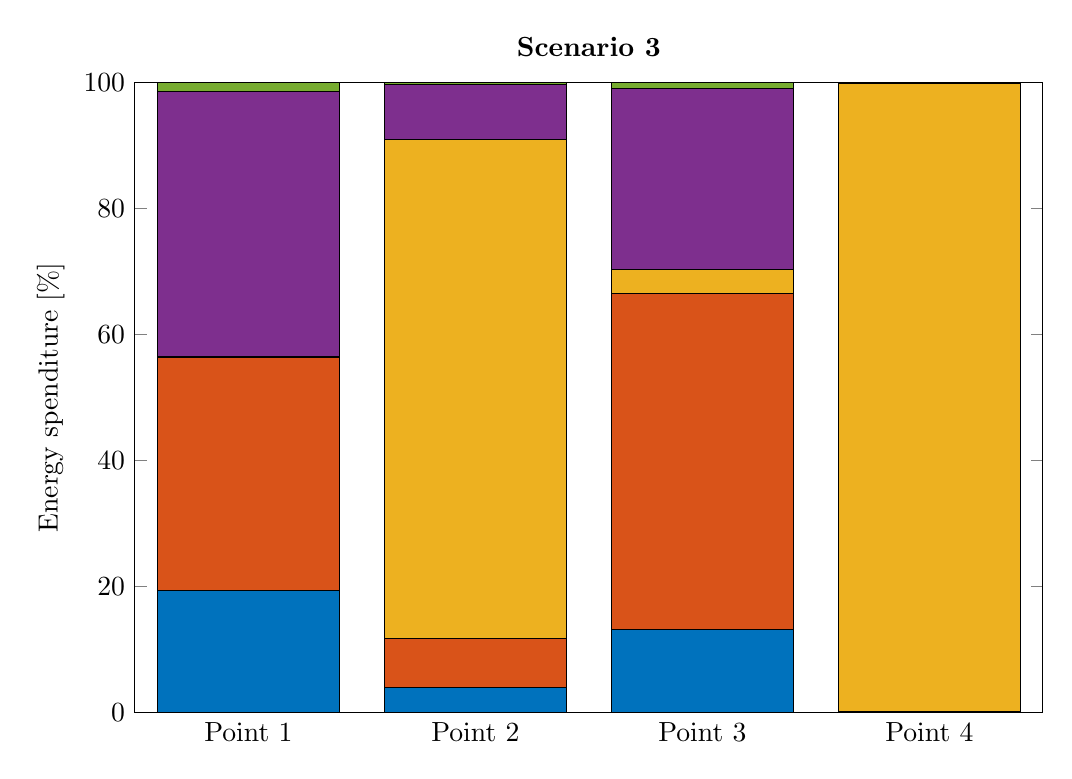
\begin{tikzpicture}

\begin{axis}[%
width=0.951\textwidth,
height=0.66\textwidth,
at={(0\textwidth,0\textwidth)},
scale only axis,
bar width=0.8,
xmin=0.5,
xmax=4.5,
xtick={1,2,3,4},
xticklabels={{Point 1},{Point 2},{Point 3},{Point 4}},
ymin=0,
ymax=100,
ylabel={Energy spenditure [\%]},
axis background/.style={fill=white},
title style={font=\bfseries},
title={Scenario 3},
y tick label style={/pgf/number format/fixed}
]
\addplot[ybar stacked,draw=black,fill=mycolor1,area legend] plot table[row sep=crcr] {%
1	19.4161813835198\\
2	4.04093241297658\\
3	13.2569703702205\\
4	0.0351236529907318\\
};
\addplot[ybar stacked,draw=black,fill=mycolor2,area legend] plot table[row sep=crcr] {%
1	36.9976571077157\\
2	7.70002241211342\\
3	53.2445264783942\\
4	0.141068601607793\\
};
\addplot[ybar stacked,draw=black,fill=mycolor3,area legend] plot table[row sep=crcr] {%
1	0.0380564339485726\\
2	79.2037705187583\\
3	3.76475029583682\\
4	99.745099592863\\
};
\addplot[ybar stacked,draw=black,fill=mycolor4,area legend] plot table[row sep=crcr] {%
1	42.1583633448444\\
2	8.77407836037336\\
3	28.7848657096895\\
4	0.076264003489293\\
};
\addplot[ybar stacked,draw=black,fill=mycolor5,area legend] plot table[row sep=crcr] 
\end{minipage}
\hfill
\begin{minipage}{0.48\textwidth}
%Scenario 3
\begin{table}[H]
\centering
\resizebox{\textwidth}{!}{
\begin{tabular}{|c|c|c|c|c|} \hline
 & Pont 1	& Pont 2	& Pont 3	& Pont 4	\\ \hline
\cellcolor{mycolor5}Idle	& 1.3897\% 	& 0.2812\%	& 0.9489\%	& 0.0024\%\\ \hline
\cellcolor{mycolor4}Release	& 42.1584\% 	& 8.7741\%	& 28.7849\%	& 0.0763\%\\ \hline
\cellcolor{mycolor3}Transmit	& 0.0381\% 	& 79.2038\%	& 3.7648\%	& 99.7451\%\\ \hline
\cellcolor{mycolor2}Attach	& 36.9977\% 	& 7.7000\%	& 53.2445\%	& 0.1411\%\\ \hline
\cellcolor{mycolor1}Sync	& 19.4162\% 	& 4.0409\%	& 13.2570\%	& 0.0351\%\\ \hline
Lifetime (years)	& 1.7891 	& 0.3723	& 1.2215	& 0.0032\\ \hline
\end{tabular}}
\end{table}
\end{minipage}
\begin{minipage}{0.48\textwidth}
\tikzsetnextfilename{eDRX_each_day_barplot}
\resizebox{\textwidth}{!}{
% This file was created by matlab2tikz.
%
%The latest updates can be retrieved from
%  http://www.mathworks.com/matlabcentral/fileexchange/22022-matlab2tikz-matlab2tikz
%where you can also make suggestions and rate matlab2tikz.
%
\definecolor{mycolor1}{rgb}{0.00000,0.44700,0.74100}%
\definecolor{mycolor2}{rgb}{0.85000,0.32500,0.09800}%
\definecolor{mycolor3}{rgb}{0.92900,0.69400,0.12500}%
\definecolor{mycolor4}{rgb}{0.49400,0.18400,0.55600}%
\definecolor{mycolor5}{rgb}{0.46600,0.67400,0.18800}%
%
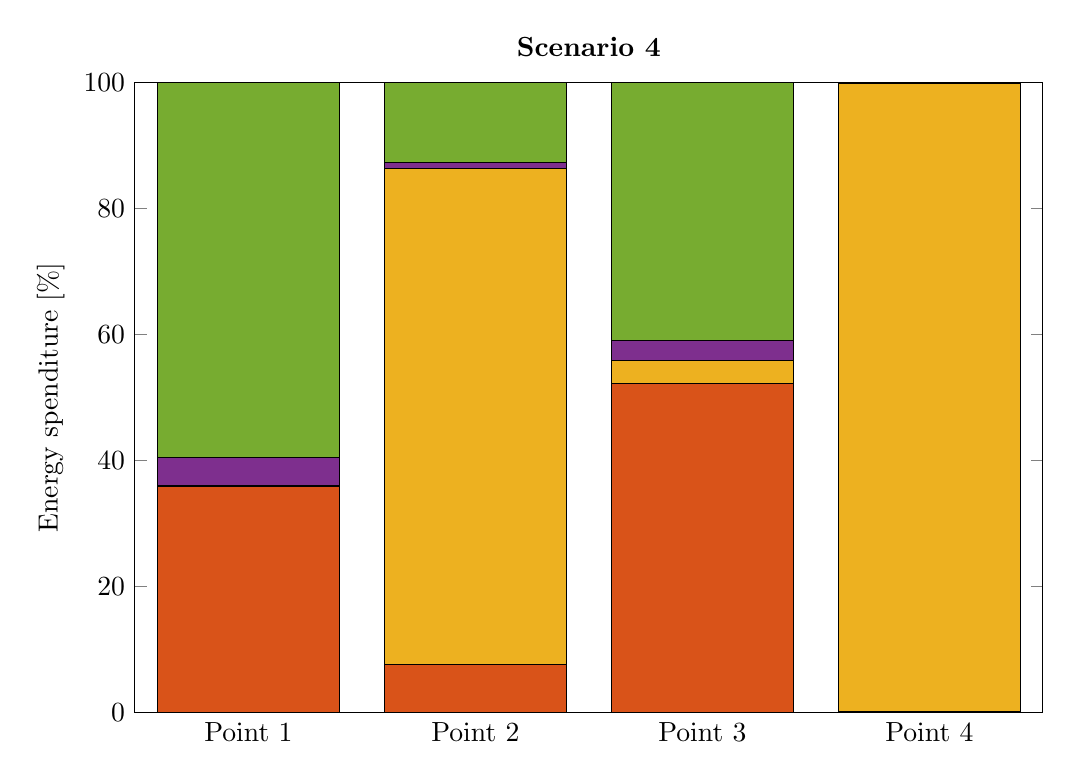
\begin{tikzpicture}

\begin{axis}[%
width=0.951\textwidth,
height=0.66\textwidth,
at={(0\textwidth,0\textwidth)},
scale only axis,
bar width=0.8,
xmin=0.5,
xmax=4.5,
xtick={1,2,3,4},
xticklabels={{Point 1},{Point 2},{Point 3},{Point 4}},
ymin=0,
ymax=100,
ylabel={Energy spenditure [\%]},
axis background/.style={fill=white},
title style={font=\bfseries},
title={Scenario 4},
y tick label style={/pgf/number format/fixed}
]
\addplot[ybar stacked,draw=black,fill=mycolor1,area legend] plot table[row sep=crcr] {%
1	0.000148933954494186\\
2	3.17039253642208e-05\\
3	0.000102603609620936\\
4	2.77194764324209e-07\\
};
\addplot[ybar stacked,draw=black,fill=mycolor2,area legend] plot table[row sep=crcr] {%
1	35.9580654744451\\
2	7.6544789797284\\
3	52.2138260888245\\
4	0.141061306426043\\
};
\addplot[ybar stacked,draw=black,fill=mycolor3,area legend] plot table[row sep=crcr] {%
1	0.0369870919032137\\
2	78.7353028476013\\
3	3.69187276544643\\
4	99.739941403004\\
};
\addplot[ybar stacked,draw=black,fill=mycolor4,area legend] plot table[row sep=crcr] {%
1	4.46951469537128\\
2	0.951436230895694\\
3	3.07913895495748\\
4	0.00831862738644596\\
};
\addplot[ybar stacked,draw=black,fill=mycolor5,area legend] plot table[row sep=crcr] 
\end{minipage}
\hfill
\begin{minipage}{0.48\textwidth}
%Scenario 4
\begin{table}[H]
\centering
\resizebox{\textwidth}{!}{
\begin{tabular}{|c|c|c|c|c|} \hline
 & Pont 1	& Pont 2	& Pont 3	& Pont 4	\\ \hline
\cellcolor{mycolor5}Idle	& 25.2881\% 	& 6.5054\%	& 18.7042\%	& 0.0603\%\\ \hline
\cellcolor{mycolor4}Release	& 31.9412\% 	& 8.2264\%	& 23.6251\%	& 0.0762\%\\ \hline
\cellcolor{mycolor3}Transmit	& 0.0288\% 	& 74.2601\%	& 3.0899\%	& 99.6874\%\\ \hline
\cellcolor{mycolor2}Attach	& 28.0312\% 	& 7.2194\%	& 43.7002\%	& 0.1410\%\\ \hline
\cellcolor{mycolor1}Sync	& 14.7106\% 	& 3.7887\%	& 10.8806\%	& 0.0351\%\\ \hline
Lifetime (years)	& 32.5317 	& 8.3785	& 24.0618	& 0.0776\\ \hline
\end{tabular}}
\end{table}
\end{minipage}
\caption{The distribution of power for each phase of a cycle. Blue is the sync phase, red is the attach phase, yellow is the transmit phase, purple is the release phase and green is the idle phase.}
\label{fig:barplot_plots}
\end{figure}

It can be seen that depending on the point and scenario the energy is used quite differently, however some commonalities can be seen. For instance if each transmission is 100 s more than 69\% of the energy is spent during the transmit phase if $P_{TX}$ is also high then more than 99\% of the energy is spent here. Another point is that with a low $T_i$, $E_{idle}$ take op less than 5\% of the used energy, while for a high $T_i$ it can take up 53\% of the energy. As mentioned when finding the energy to release the device from the network, the model fails to predict how it scales with $P_{TX}$ and a 95\% limit was taken as a worst case estimate. This shows here as the energy spent during the attach phase is actually less than that used during the release phase when $P_{TX}$ is set low, which in reality should not be the case. It can also be seen here why a low $T_i$ makes eDRX more feasible than PSM, as the energy spent to synchronize is fairly high, while for high $T_i$ the energy spent on paging will be even higher. Another thing to take from this is also that even with a $T_i$ of 24 hours if maximum $P_{TX}$ is used, $T_{transmit}$ should be less than 0.4677 s and 0.4571 s for eDRX and PSM respectively to get a battery lifetime of 10 years. 


With this analysis it can be concluded that a device can achieve a battery lifetime of more than 10 years, but in extreme situations the repetition value will increase which makes $T_{transmit}$ increase, and also the needed $P_{TX}$ would be high. When these parameters are high it has been shown that a battery lifetime might not even exceed one year independently on all other parameters. To combat this when designing the devices, focus should be put on decreasing $T_{transmit}$ as much as possible, and also on increasing $T_i$. 
